%%%%%%%%%%%%%%%%%%%%%%%%%%%%%%%%%%%%%%%%%%%%%%%%%%%%%%%%%%%%%%%%%
\chapter{Alternative Algorithms}  \newpage
%%%%%%%%%%%%%%%%%%%%%%%%%%%%%%%%%%%%%%%%%%%%%%%%%%%%%%%%%%%%%%%%%
% Load model-specific values
% Model 1 Calibrated Values
% Generated: 2025-10-02 01:58:23.185499
% Model: Linear with Outlier Removal

% Core Metrics
\renewcommand{\ModelOneRSquaredTrain}{0.2383}
\renewcommand{\ModelOneRSquaredTest}{0.2178}
\renewcommand{\ModelOneRMSETrain}{39,238}
\renewcommand{\ModelOneRMSETest}{39,500}
\renewcommand{\ModelOneMAETrain}{27,831}
\renewcommand{\ModelOneMAETest}{27,912}
\renewcommand{\ModelOneMAPETrain}{85.2}
\renewcommand{\ModelOneMAPETest}{84.8}
\renewcommand{\ModelOneCVMean}{0.2372}
\renewcommand{\ModelOneCVStd}{0.0196}
\renewcommand{\ModelOneWithinOneK}{2.4}
\renewcommand{\ModelOneWithinTwoK}{4.9}
\renewcommand{\ModelOneWithinFiveK}{15.8}
\renewcommand{\ModelOneWithinTenK}{28.5}
\renewcommand{\ModelOneWithinTwentyK}{49.5}
\renewcommand{\ModelOneTrainingSamples}{27,339}
\renewcommand{\ModelOneTestSamples}{6,834}

% Subgroup Metrics
\renewcommand{\ModelOneSubgrouplivingFHN}{5,941}
\renewcommand{\ModelOneSubgrouplivingFHRSquared}{0.222}
\renewcommand{\ModelOneSubgrouplivingFHRMSE}{39,928}
\renewcommand{\ModelOneSubgrouplivingFHBias}{-7,487}
\renewcommand{\ModelOneSubgrouplivingILSLN}{893}
\renewcommand{\ModelOneSubgrouplivingILSLRSquared}{0.179}
\renewcommand{\ModelOneSubgrouplivingILSLRMSE}{36,524}
\renewcommand{\ModelOneSubgrouplivingILSLBias}{-3,272}
\renewcommand{\ModelOneSubgroupageAgeUnderTwentyOneN}{694}
\renewcommand{\ModelOneSubgroupageAgeUnderTwentyOneRSquared}{0.138}
\renewcommand{\ModelOneSubgroupageAgeUnderTwentyOneRMSE}{34,649}
\renewcommand{\ModelOneSubgroupageAgeUnderTwentyOneBias}{-8,152}
\renewcommand{\ModelOneSubgroupageAgeTwentyOneToThirtyN}{1,797}
\renewcommand{\ModelOneSubgroupageAgeTwentyOneToThirtyRSquared}{0.161}
\renewcommand{\ModelOneSubgroupageAgeTwentyOneToThirtyRMSE}{44,751}
\renewcommand{\ModelOneSubgroupageAgeTwentyOneToThirtyBias}{-7,785}
\renewcommand{\ModelOneSubgroupageAgeThirtyOnePlusN}{4,343}
\renewcommand{\ModelOneSubgroupageAgeThirtyOnePlusRSquared}{0.218}
\renewcommand{\ModelOneSubgroupageAgeThirtyOnePlusRMSE}{37,876}
\renewcommand{\ModelOneSubgroupageAgeThirtyOnePlusBias}{-6,391}
\renewcommand{\ModelOneSubgroupcostQOneLowN}{1,709}
\renewcommand{\ModelOneSubgroupcostQOneLowRSquared}{-10.000}
\renewcommand{\ModelOneSubgroupcostQOneLowRMSE}{31,272}
\renewcommand{\ModelOneSubgroupcostQOneLowBias}{+24,162}
\renewcommand{\ModelOneSubgroupcostQTwoN}{1,708}
\renewcommand{\ModelOneSubgroupcostQTwoRSquared}{-6.029}
\renewcommand{\ModelOneSubgroupcostQTwoRMSE}{20,461}
\renewcommand{\ModelOneSubgroupcostQTwoBias}{+9,755}
\renewcommand{\ModelOneSubgroupcostQThreeN}{1,708}
\renewcommand{\ModelOneSubgroupcostQThreeRSquared}{-4.117}
\renewcommand{\ModelOneSubgroupcostQThreeRMSE}{26,401}
\renewcommand{\ModelOneSubgroupcostQThreeBias}{-13,739}
\renewcommand{\ModelOneSubgroupcostQFourHighN}{1,709}
\renewcommand{\ModelOneSubgroupcostQFourHighRSquared}{-2.230}
\renewcommand{\ModelOneSubgroupcostQFourHighRMSE}{64,390}
\renewcommand{\ModelOneSubgroupcostQFourHighBias}{-47,917}

% Variance Metrics
\renewcommand{\ModelOneCVActual}{1.010}
\renewcommand{\ModelOneCVPredicted}{0.692}
\renewcommand{\ModelOnePredictionInterval}{152,432}
\renewcommand{\ModelOneBudgetActualCorr}{0.498}
\renewcommand{\ModelOneQuarterlyVariance}{87.9}
\renewcommand{\ModelOneAnnualAdjustmentRate}{92.4}

% Population Scenarios
\renewcommand{\ModelOnePopcurrentbaselineClients}{32,188}
\renewcommand{\ModelOnePopcurrentbaselineAvgAlloc}{37,280}
\renewcommand{\ModelOnePopcurrentbaselineWaitlistChange}{+0}
\renewcommand{\ModelOnePopcurrentbaselineWaitlistPct}{+0.0}
\renewcommand{\ModelOnePopmodelbalancedClients}{32,831}
\renewcommand{\ModelOnePopmodelbalancedAvgAlloc}{36,534}
\renewcommand{\ModelOnePopmodelbalancedWaitlistChange}{+643}
\renewcommand{\ModelOnePopmodelbalancedWaitlistPct}{+2.0}
\renewcommand{\ModelOnePopmodelefficiencyClients}{33,797}
\renewcommand{\ModelOnePopmodelefficiencyAvgAlloc}{35,416}
\renewcommand{\ModelOnePopmodelefficiencyWaitlistChange}{+1,609}
\renewcommand{\ModelOnePopmodelefficiencyWaitlistPct}{+5.0}
\renewcommand{\ModelOnePopcategoryfocusedClients}{27,359}
\renewcommand{\ModelOnePopcategoryfocusedAvgAlloc}{43,990}
\renewcommand{\ModelOnePopcategoryfocusedWaitlistChange}{-4,828}
\renewcommand{\ModelOnePopcategoryfocusedWaitlistPct}{-15.0}
\renewcommand{\ModelOnePoppopulationmaximizedClients}{37,016}
\renewcommand{\ModelOnePoppopulationmaximizedAvgAlloc}{32,434}
\renewcommand{\ModelOnePoppopulationmaximizedWaitlistChange}{+4,828}
\renewcommand{\ModelOnePoppopulationmaximizedWaitlistPct}{+15.0}

% Model 1 Specific Metrics
\renewcommand{\ModelOneOutliersRemoved}{2570}
\renewcommand{\ModelOneOutlierPercentage}{9.4}
\renewcommand{\ModelOneTransformation}{Square Root}
\renewcommand{\ModelOneNumFeatures}{26}
\renewcommand{\ModelOnePredictionFloor}{5,000}

% Feature Selection Specific Values
\renewcommand{\ModelOneFeatureSelection}{True}
\renewcommand{\ModelOneFiscalYears}{2024}
\renewcommand{\ModelOneMIScoreTop}{0.272}
\renewcommand{\ModelOneVarianceExplained}{89.0}

% Model 2 Actual Values
% Generated: 2025-10-10 12:43:06

\renewcommand{\ModelTwoRSquaredTrain}{0.4469}
\renewcommand{\ModelTwoRSquaredTest}{0.4386}
\renewcommand{\ModelTwoRMSETrain}{33,435.41}
\renewcommand{\ModelTwoRMSETest}{33,463.23}
\renewcommand{\ModelTwoRMSETrainSqrt}{33435.41}
\renewcommand{\ModelTwoRMSETestSqrt}{33463.23}
\renewcommand{\ModelTwoMAETrain}{23,576.23}
\renewcommand{\ModelTwoMAETest}{23,279.01}
\renewcommand{\ModelTwoMAPETrain}{427.92}
\renewcommand{\ModelTwoMAPETest}{445.86}
\renewcommand{\ModelTwoCVMean}{0.4432}
\renewcommand{\ModelTwoCVStd}{0.0218}
\renewcommand{\ModelTwoCVCILower}{0.4005}
\renewcommand{\ModelTwoCVCIUpper}{0.4859}
\renewcommand{\ModelTwoTrainingSamples}{27,339}
\renewcommand{\ModelTwoTestSamples}{6,834}
\renewcommand{\ModelTwoWithinOneK}{3.06}
\renewcommand{\ModelTwoWithinTwoK}{6.20}
\renewcommand{\ModelTwoWithinFiveK}{15.96}
\renewcommand{\ModelTwoWithinTenK}{32.54}
\renewcommand{\ModelTwoWithinTwentyK}{58.17}
\renewcommand{\ModelTwoSubgroupLivingFHN}{3,767}
\renewcommand{\ModelTwoSubgroupLivingFHRSquared}{0.1568}
\renewcommand{\ModelTwoSubgroupLivingFHRMSE}{29,245.76}
\renewcommand{\ModelTwoSubgroupLivingFHBias}{-1,093.72}
\renewcommand{\ModelTwoSubgroupLivingILSLN}{893}
\renewcommand{\ModelTwoSubgroupLivingILSLRSquared}{0.2819}
\renewcommand{\ModelTwoSubgroupLivingILSLRMSE}{34,160.69}
\renewcommand{\ModelTwoSubgroupLivingILSLBias}{-1,858.10}
\renewcommand{\ModelTwoSubgroupLivingRHOneFourN}{2,174}
\renewcommand{\ModelTwoSubgroupLivingRHOneFourRSquared}{0.0741}
\renewcommand{\ModelTwoSubgroupLivingRHOneFourRMSE}{39,480.14}
\renewcommand{\ModelTwoSubgroupLivingRHOneFourBias}{5,288.21}
\renewcommand{\ModelTwoSubgroupAgeAgeUnderTwentyOneN}{694}
\renewcommand{\ModelTwoSubgroupAgeAgeUnderTwentyOneRSquared}{0.3847}
\renewcommand{\ModelTwoSubgroupAgeAgeUnderTwentyOneRMSE}{29,267.07}
\renewcommand{\ModelTwoSubgroupAgeAgeUnderTwentyOneBias}{-5,269.63}
\renewcommand{\ModelTwoSubgroupAgeAgeTwentyOneToThirtyN}{1,797}
\renewcommand{\ModelTwoSubgroupAgeAgeTwentyOneToThirtyRSquared}{0.4346}
\renewcommand{\ModelTwoSubgroupAgeAgeTwentyOneToThirtyRMSE}{36,739.09}
\renewcommand{\ModelTwoSubgroupAgeAgeTwentyOneToThirtyBias}{1,780.25}
\renewcommand{\ModelTwoSubgroupAgeAgeThirtyOnePlusN}{4,343}
\renewcommand{\ModelTwoSubgroupAgeAgeThirtyOnePlusRSquared}{0.4185}
\renewcommand{\ModelTwoSubgroupAgeAgeThirtyOnePlusRMSE}{32,660.30}
\renewcommand{\ModelTwoSubgroupAgeAgeThirtyOnePlusBias}{1,421.89}
\renewcommand{\ModelTwoSubgroupCostQOneLowN}{1,709}
\renewcommand{\ModelTwoSubgroupCostQOneLowRSquared}{-10.0000}
\renewcommand{\ModelTwoSubgroupCostQOneLowRMSE}{25,866.48}
\renewcommand{\ModelTwoSubgroupCostQOneLowBias}{20,962.33}
\renewcommand{\ModelTwoSubgroupCostQTwoN}{1,708}
\renewcommand{\ModelTwoSubgroupCostQTwoRSquared}{-5.0607}
\renewcommand{\ModelTwoSubgroupCostQTwoRMSE}{18,998.46}
\renewcommand{\ModelTwoSubgroupCostQTwoBias}{8,891.48}
\renewcommand{\ModelTwoSubgroupCostQThreeN}{1,708}
\renewcommand{\ModelTwoSubgroupCostQThreeRSquared}{-3.7821}
\renewcommand{\ModelTwoSubgroupCostQThreeRMSE}{25,523.51}
\renewcommand{\ModelTwoSubgroupCostQThreeBias}{-3,936.44}
\renewcommand{\ModelTwoSubgroupCostQFourHighN}{1,709}
\renewcommand{\ModelTwoSubgroupCostQFourHighRSquared}{-1.1793}
\renewcommand{\ModelTwoSubgroupCostQFourHighRMSE}{52,886.36}
\renewcommand{\ModelTwoSubgroupCostQFourHighBias}{-22,569.10}
\renewcommand{\ModelTwoCVActual}{1.0101}
\renewcommand{\ModelTwoCVPredicted}{0.7915}
\renewcommand{\ModelTwoPredictionInterval}{65,567.43}
\renewcommand{\ModelTwoBudgetActualCorr}{0.6741}
\renewcommand{\ModelTwoPopcurrentbaselineClients}{26,635}
\renewcommand{\ModelTwoPopcurrentbaselineAvgAlloc}{45,052.77}
\renewcommand{\ModelTwoPopcurrentbaselineWaitlistChange}{0}
\renewcommand{\ModelTwoPopcurrentbaselineWaitlistPct}{0.0}
\renewcommand{\ModelTwoPopmodelbalancedClients}{27,167}
\renewcommand{\ModelTwoPopmodelbalancedAvgAlloc}{44,151.71}
\renewcommand{\ModelTwoPopmodelbalancedWaitlistChange}{532}
\renewcommand{\ModelTwoPopmodelbalancedWaitlistPct}{2.0}
\renewcommand{\ModelTwoPopmodelefficiencyClients}{27,966}
\renewcommand{\ModelTwoPopmodelefficiencyAvgAlloc}{42,800.13}
\renewcommand{\ModelTwoPopmodelefficiencyWaitlistChange}{1,331}
\renewcommand{\ModelTwoPopmodelefficiencyWaitlistPct}{5.0}
\renewcommand{\ModelTwoPopcategoryfocusedClients}{22,639}
\renewcommand{\ModelTwoPopcategoryfocusedAvgAlloc}{53,162.27}
\renewcommand{\ModelTwoPopcategoryfocusedWaitlistChange}{-3,995}
\renewcommand{\ModelTwoPopcategoryfocusedWaitlistPct}{-15.0}

% Outlier Diagnostics (not used)
\renewcommand{\ModelTwoStudentizedResidualsMean}{N/A}
\renewcommand{\ModelTwoStudentizedResidualsStd}{N/A}
\renewcommand{\ModelTwoPctWithinThreshold}{N/A}
\renewcommand{\ModelTwoOutliersRemoved}{0}
\renewcommand{\ModelTwoOutlierPct}{0.00}

% Model Configuration
\renewcommand{\ModelTwoNumFeatures}{57}

% Model 3 Actual Values
% Generated: 2025-10-14 14:58:34

\renewcommand{\ModelThreeRSquaredTrain}{0.4476}
\renewcommand{\ModelThreeRSquaredTest}{0.4317}
\renewcommand{\ModelThreeRMSETrain}{33,414.82}
\renewcommand{\ModelThreeRMSETest}{33,666.51}
\renewcommand{\ModelThreeRMSETrainSqrt}{78.84}
\renewcommand{\ModelThreeRMSETestSqrt}{79.50}
\renewcommand{\ModelThreeMAETrain}{21,790.51}
\renewcommand{\ModelThreeMAETest}{21,781.59}
\renewcommand{\ModelThreeMAPETrain}{295.28}
\renewcommand{\ModelThreeMAPETest}{304.22}
\renewcommand{\ModelThreeCVMean}{0.4468}
\renewcommand{\ModelThreeCVStd}{0.0171}
\renewcommand{\ModelThreeCVCILower}{0.4132}
\renewcommand{\ModelThreeCVCIUpper}{0.4804}
\renewcommand{\ModelThreeTrainingSamples}{27,339}
\renewcommand{\ModelThreeTestSamples}{6,834}
\renewcommand{\ModelThreeWithinOneK}{4.01}
\renewcommand{\ModelThreeWithinTwoK}{8.75}
\renewcommand{\ModelThreeWithinFiveK}{21.44}
\renewcommand{\ModelThreeWithinTenK}{39.11}
\renewcommand{\ModelThreeWithinTwentyK}{65.19}
\renewcommand{\ModelThreeSubgroupLivingFHN}{3,767}
\renewcommand{\ModelThreeSubgroupLivingFHRSquared}{-0.0020}
\renewcommand{\ModelThreeSubgroupLivingFHRMSE}{31,879.76}
\renewcommand{\ModelThreeSubgroupLivingFHBias}{-9,939.40}
\renewcommand{\ModelThreeSubgroupLivingILSLN}{893}
\renewcommand{\ModelThreeSubgroupLivingILSLRSquared}{0.2827}
\renewcommand{\ModelThreeSubgroupLivingILSLRMSE}{34,143.24}
\renewcommand{\ModelThreeSubgroupLivingILSLBias}{-5,789.51}
\renewcommand{\ModelThreeSubgroupLivingRHOneFourN}{2,174}
\renewcommand{\ModelThreeSubgroupLivingRHOneFourRSquared}{0.2141}
\renewcommand{\ModelThreeSubgroupLivingRHOneFourRMSE}{36,374.24}
\renewcommand{\ModelThreeSubgroupLivingRHOneFourBias}{-2,788.13}
\renewcommand{\ModelThreeSubgroupAgeAgeUnderTwentyOneN}{694}
\renewcommand{\ModelThreeSubgroupAgeAgeUnderTwentyOneRSquared}{0.5075}
\renewcommand{\ModelThreeSubgroupAgeAgeUnderTwentyOneRMSE}{26,184.14}
\renewcommand{\ModelThreeSubgroupAgeAgeUnderTwentyOneBias}{-4,240.70}
\renewcommand{\ModelThreeSubgroupAgeAgeTwentyOneToThirtyN}{1,797}
\renewcommand{\ModelThreeSubgroupAgeAgeTwentyOneToThirtyRSquared}{0.3832}
\renewcommand{\ModelThreeSubgroupAgeAgeTwentyOneToThirtyRMSE}{38,373.30}
\renewcommand{\ModelThreeSubgroupAgeAgeTwentyOneToThirtyBias}{-9,770.89}
\renewcommand{\ModelThreeSubgroupAgeAgeThirtyOnePlusN}{4,343}
\renewcommand{\ModelThreeSubgroupAgeAgeThirtyOnePlusRSquared}{0.4196}
\renewcommand{\ModelThreeSubgroupAgeAgeThirtyOnePlusRMSE}{32,629.67}
\renewcommand{\ModelThreeSubgroupAgeAgeThirtyOnePlusBias}{-6,486.72}
\renewcommand{\ModelThreeSubgroupCostQOneLowN}{1,709}
\renewcommand{\ModelThreeSubgroupCostQOneLowRSquared}{-10.0000}
\renewcommand{\ModelThreeSubgroupCostQOneLowRMSE}{19,666.66}
\renewcommand{\ModelThreeSubgroupCostQOneLowBias}{13,349.85}
\renewcommand{\ModelThreeSubgroupCostQTwoN}{1,708}
\renewcommand{\ModelThreeSubgroupCostQTwoRSquared}{-3.5980}
\renewcommand{\ModelThreeSubgroupCostQTwoRMSE}{16,547.81}
\renewcommand{\ModelThreeSubgroupCostQTwoBias}{2,784.62}
\renewcommand{\ModelThreeSubgroupCostQThreeN}{1,708}
\renewcommand{\ModelThreeSubgroupCostQThreeRSquared}{-4.3906}
\renewcommand{\ModelThreeSubgroupCostQThreeRMSE}{27,098.83}
\renewcommand{\ModelThreeSubgroupCostQThreeBias}{-10,252.18}
\renewcommand{\ModelThreeSubgroupCostQFourHighN}{1,709}
\renewcommand{\ModelThreeSubgroupCostQFourHighRSquared}{-1.4450}
\renewcommand{\ModelThreeSubgroupCostQFourHighRMSE}{56,018.24}
\renewcommand{\ModelThreeSubgroupCostQFourHighBias}{-34,367.15}
\renewcommand{\ModelThreeCVActual}{1.0101}
\renewcommand{\ModelThreeCVPredicted}{0.8788}
\renewcommand{\ModelThreePredictionInterval}{64,492.87}
\renewcommand{\ModelThreeBudgetActualCorr}{0.6781}
\renewcommand{\ModelThreePopcurrentbaselineClients}{32,350}
\renewcommand{\ModelThreePopcurrentbaselineAvgAlloc}{37,093.98}
\renewcommand{\ModelThreePopcurrentbaselineWaitlistChange}{0}
\renewcommand{\ModelThreePopcurrentbaselineWaitlistPct}{0.0}
\renewcommand{\ModelThreePopmodelbalancedClients}{32,997}
\renewcommand{\ModelThreePopmodelbalancedAvgAlloc}{36,352.10}
\renewcommand{\ModelThreePopmodelbalancedWaitlistChange}{647}
\renewcommand{\ModelThreePopmodelbalancedWaitlistPct}{2.0}
\renewcommand{\ModelThreePopmodelefficiencyClients}{33,967}
\renewcommand{\ModelThreePopmodelefficiencyAvgAlloc}{35,239.28}
\renewcommand{\ModelThreePopmodelefficiencyWaitlistChange}{1,617}
\renewcommand{\ModelThreePopmodelefficiencyWaitlistPct}{5.0}
\renewcommand{\ModelThreePopcategoryfocusedClients}{27,497}
\renewcommand{\ModelThreePopcategoryfocusedAvgAlloc}{43,770.89}
\renewcommand{\ModelThreePopcategoryfocusedWaitlistChange}{-4,852}
\renewcommand{\ModelThreePopcategoryfocusedWaitlistPct}{-15.0}

% Outlier Diagnostics (not used)
\renewcommand{\ModelThreeStudentizedResidualsMean}{N/A}
\renewcommand{\ModelThreeStudentizedResidualsStd}{N/A}
\renewcommand{\ModelThreePctWithinThreshold}{N/A}
\renewcommand{\ModelThreeOutliersRemoved}{0}
\renewcommand{\ModelThreeOutlierPct}{0.00}

% Model Configuration
\renewcommand{\ModelThreeNumFeatures}{21}

% Model 3 Robust Regression Specific Values
\renewcommand{\ModelThreeEpsilon}{1.35}
\renewcommand{\ModelThreeScaleEstimate}{49.1719}
\renewcommand{\ModelThreeNumIterations}{32}
\renewcommand{\ModelThreeConverged}{Yes}
\renewcommand{\ModelThreeParameters}{22}
\renewcommand{\ModelThreeMeanWeight}{0.8770}
\renewcommand{\ModelThreeMedianWeight}{1.0000}
\renewcommand{\ModelThreeMinWeight}{0.1565}
\renewcommand{\ModelThreeFullWeightPct}{63.6}
\renewcommand{\ModelThreeOutliersDetected}{9938}
\renewcommand{\ModelThreeOutlierPercentage}{36.4}
\renewcommand{\ModelThreeWithinOneK}{4.0}
\renewcommand{\ModelThreeWithinTwoK}{8.8}
\renewcommand{\ModelThreeWithinFiveK}{21.4}
\renewcommand{\ModelThreeWithinTenK}{39.1}
\renewcommand{\ModelThreeWithinTwentyK}{65.2}

% Model 4 Actual Values
% Generated: 2025-10-14 22:47:08

\renewcommand{\ModelFourRSquaredTrain}{0.4731}
\renewcommand{\ModelFourRSquaredTest}{0.4562}
\renewcommand{\ModelFourRMSETrain}{32,633.88}
\renewcommand{\ModelFourRMSETest}{32,933.69}
\renewcommand{\ModelFourRMSETrainSqrt}{78.04}
\renewcommand{\ModelFourRMSETestSqrt}{78.77}
\renewcommand{\ModelFourMAETrain}{21,742.19}
\renewcommand{\ModelFourMAETest}{21,707.50}
\renewcommand{\ModelFourMAPETrain}{341.72}
\renewcommand{\ModelFourMAPETest}{351.38}
\renewcommand{\ModelFourCVMean}{0.4710}
\renewcommand{\ModelFourCVStd}{0.0180}
\renewcommand{\ModelFourCVCILower}{0.4356}
\renewcommand{\ModelFourCVCIUpper}{0.5064}
\renewcommand{\ModelFourTrainingSamples}{27,339}
\renewcommand{\ModelFourTestSamples}{6,834}
\renewcommand{\ModelFourWithinOneK}{4.26}
\renewcommand{\ModelFourWithinTwoK}{8.41}
\renewcommand{\ModelFourWithinFiveK}{19.92}
\renewcommand{\ModelFourWithinTenK}{37.06}
\renewcommand{\ModelFourWithinTwentyK}{63.81}
\renewcommand{\ModelFourSubgroupLivingFHN}{3,767}
\renewcommand{\ModelFourSubgroupLivingFHRSquared}{0.0803}
\renewcommand{\ModelFourSubgroupLivingFHRMSE}{30,542.90}
\renewcommand{\ModelFourSubgroupLivingFHBias}{-6,480.80}
\renewcommand{\ModelFourSubgroupLivingILSLN}{893}
\renewcommand{\ModelFourSubgroupLivingILSLRSquared}{0.1960}
\renewcommand{\ModelFourSubgroupLivingILSLRMSE}{36,147.39}
\renewcommand{\ModelFourSubgroupLivingILSLBias}{-8,204.50}
\renewcommand{\ModelFourSubgroupLivingRHOneFourN}{2,174}
\renewcommand{\ModelFourSubgroupLivingRHOneFourRSquared}{0.2537}
\renewcommand{\ModelFourSubgroupLivingRHOneFourRMSE}{35,445.68}
\renewcommand{\ModelFourSubgroupLivingRHOneFourBias}{-4,436.42}
\renewcommand{\ModelFourSubgroupAgeAgeUnderTwentyOneN}{694}
\renewcommand{\ModelFourSubgroupAgeAgeUnderTwentyOneRSquared}{0.5208}
\renewcommand{\ModelFourSubgroupAgeAgeUnderTwentyOneRMSE}{25,828.52}
\renewcommand{\ModelFourSubgroupAgeAgeUnderTwentyOneBias}{-3,469.18}
\renewcommand{\ModelFourSubgroupAgeAgeTwentyOneToThirtyN}{1,797}
\renewcommand{\ModelFourSubgroupAgeAgeTwentyOneToThirtyRSquared}{0.4311}
\renewcommand{\ModelFourSubgroupAgeAgeTwentyOneToThirtyRMSE}{36,853.18}
\renewcommand{\ModelFourSubgroupAgeAgeTwentyOneToThirtyBias}{-5,890.51}
\renewcommand{\ModelFourSubgroupAgeAgeThirtyOnePlusN}{4,343}
\renewcommand{\ModelFourSubgroupAgeAgeThirtyOnePlusRSquared}{0.4341}
\renewcommand{\ModelFourSubgroupAgeAgeThirtyOnePlusRMSE}{32,220.61}
\renewcommand{\ModelFourSubgroupAgeAgeThirtyOnePlusBias}{-6,537.35}
\renewcommand{\ModelFourSubgroupCostQOneLowN}{1,709}
\renewcommand{\ModelFourSubgroupCostQOneLowRSquared}{-10.0000}
\renewcommand{\ModelFourSubgroupCostQOneLowRMSE}{20,913.43}
\renewcommand{\ModelFourSubgroupCostQOneLowBias}{15,976.68}
\renewcommand{\ModelFourSubgroupCostQTwoN}{1,708}
\renewcommand{\ModelFourSubgroupCostQTwoRSquared}{-3.3819}
\renewcommand{\ModelFourSubgroupCostQTwoRMSE}{16,154.20}
\renewcommand{\ModelFourSubgroupCostQTwoBias}{4,519.52}
\renewcommand{\ModelFourSubgroupCostQThreeN}{1,708}
\renewcommand{\ModelFourSubgroupCostQThreeRSquared}{-3.4885}
\renewcommand{\ModelFourSubgroupCostQThreeRMSE}{24,727.48}
\renewcommand{\ModelFourSubgroupCostQThreeBias}{-10,263.15}
\renewcommand{\ModelFourSubgroupCostQFourHighN}{1,709}
\renewcommand{\ModelFourSubgroupCostQFourHighRSquared}{-1.3593}
\renewcommand{\ModelFourSubgroupCostQFourHighRMSE}{55,027.04}
\renewcommand{\ModelFourSubgroupCostQFourHighBias}{-34,452.09}
\renewcommand{\ModelFourCVActual}{1.0101}
\renewcommand{\ModelFourCVPredicted}{0.8046}
\renewcommand{\ModelFourPredictionInterval}{63,449.43}
\renewcommand{\ModelFourBudgetActualCorr}{0.6889}
\renewcommand{\ModelFourPopcurrentbaselineClients}{31,446}
\renewcommand{\ModelFourPopcurrentbaselineAvgAlloc}{38,160.49}
\renewcommand{\ModelFourPopcurrentbaselineWaitlistChange}{0}
\renewcommand{\ModelFourPopcurrentbaselineWaitlistPct}{0.0}
\renewcommand{\ModelFourPopmodelbalancedClients}{32,074}
\renewcommand{\ModelFourPopmodelbalancedAvgAlloc}{37,397.28}
\renewcommand{\ModelFourPopmodelbalancedWaitlistChange}{628}
\renewcommand{\ModelFourPopmodelbalancedWaitlistPct}{2.0}
\renewcommand{\ModelFourPopmodelefficiencyClients}{33,018}
\renewcommand{\ModelFourPopmodelefficiencyAvgAlloc}{36,252.47}
\renewcommand{\ModelFourPopmodelefficiencyWaitlistChange}{1,572}
\renewcommand{\ModelFourPopmodelefficiencyWaitlistPct}{5.0}
\renewcommand{\ModelFourPopcategoryfocusedClients}{26,729}
\renewcommand{\ModelFourPopcategoryfocusedAvgAlloc}{45,029.38}
\renewcommand{\ModelFourPopcategoryfocusedWaitlistChange}{-4,716}
\renewcommand{\ModelFourPopcategoryfocusedWaitlistPct}{-15.0}

% Outlier Diagnostics (not used)
\renewcommand{\ModelFourStudentizedResidualsMean}{N/A}
\renewcommand{\ModelFourStudentizedResidualsStd}{N/A}
\renewcommand{\ModelFourPctWithinThreshold}{N/A}
\renewcommand{\ModelFourOutliersRemoved}{0}
\renewcommand{\ModelFourOutlierPct}{0.00}

% Model Configuration
\renewcommand{\ModelFourNumFeatures}{57}

% Model 4 WLS-Specific Values
\renewcommand{\ModelFourWeightedRSquared}{0.551}
\renewcommand{\ModelFourWeightedRMSE}{5,084}
\renewcommand{\ModelFourEfficiencyRatio}{1.19}
\renewcommand{\ModelFourBreuschPagan}{2861.10}
\renewcommand{\ModelFourBreuschPaganPValue}{1.000000}
\renewcommand{\ModelFourBreuschPaganRTwo}{0.1047}
\renewcommand{\ModelFourBreuschPaganAfter}{1988.71}
\renewcommand{\ModelFourBreuschPaganPValueAfter}{1.000000}
\renewcommand{\ModelFourBreuschPaganRTwoAfter}{0.0727}
\renewcommand{\ModelFourWeightMin}{0.2}
\renewcommand{\ModelFourWeightMax}{5.0}
\renewcommand{\ModelFourWeightMean}{1.420}
\renewcommand{\ModelFourWeightAtMinPct}{0.0}
\renewcommand{\ModelFourWeightAboveThreePct}{10.6}
\renewcommand{\ModelFourVarPredictors}{Intercept, ILSL, RH1, RH2, RH3, RH4, bsum, Age21_30, Age31Plus, FH_x_BSum}

% Model 5 Actual Values
% Generated: 2025-10-15 13:36:08

\renewcommand{\ModelFiveRSquaredTrain}{0.4940}
\renewcommand{\ModelFiveRSquaredTest}{0.4772}
\renewcommand{\ModelFiveRMSETrain}{31,979.01}
\renewcommand{\ModelFiveRMSETest}{32,290.80}
\renewcommand{\ModelFiveRMSETrainSqrt}{32031.46}
\renewcommand{\ModelFiveRMSETestSqrt}{32336.38}
\renewcommand{\ModelFiveMAETrain}{22,498.99}
\renewcommand{\ModelFiveMAETest}{22,479.38}
\renewcommand{\ModelFiveMAPETrain}{461.85}
\renewcommand{\ModelFiveMAPETest}{473.99}
\renewcommand{\ModelFiveCVMean}{0.4918}
\renewcommand{\ModelFiveCVStd}{0.0164}
\renewcommand{\ModelFiveCVCILower}{0.4596}
\renewcommand{\ModelFiveCVCIUpper}{0.5240}
\renewcommand{\ModelFiveTrainingSamples}{27,339}
\renewcommand{\ModelFiveTestSamples}{6,834}
\renewcommand{\ModelFiveWithinOneK}{4.65}
\renewcommand{\ModelFiveWithinTwoK}{8.31}
\renewcommand{\ModelFiveWithinFiveK}{17.93}
\renewcommand{\ModelFiveWithinTenK}{32.95}
\renewcommand{\ModelFiveWithinTwentyK}{58.08}
\renewcommand{\ModelFiveSubgroupLivingFHN}{3,767}
\renewcommand{\ModelFiveSubgroupLivingFHRSquared}{0.1280}
\renewcommand{\ModelFiveSubgroupLivingFHRMSE}{29,739.60}
\renewcommand{\ModelFiveSubgroupLivingFHBias}{-10.66}
\renewcommand{\ModelFiveSubgroupLivingILSLN}{893}
\renewcommand{\ModelFiveSubgroupLivingILSLRSquared}{0.2710}
\renewcommand{\ModelFiveSubgroupLivingILSLRMSE}{34,419.95}
\renewcommand{\ModelFiveSubgroupLivingILSLBias}{119.68}
\renewcommand{\ModelFiveSubgroupLivingRHOneFourN}{2,174}
\renewcommand{\ModelFiveSubgroupLivingRHOneFourRSquared}{0.2524}
\renewcommand{\ModelFiveSubgroupLivingRHOneFourRMSE}{35,476.24}
\renewcommand{\ModelFiveSubgroupLivingRHOneFourBias}{766.81}
\renewcommand{\ModelFiveSubgroupAgeAgeUnderTwentyOneN}{694}
\renewcommand{\ModelFiveSubgroupAgeAgeUnderTwentyOneRSquared}{0.5123}
\renewcommand{\ModelFiveSubgroupAgeAgeUnderTwentyOneRMSE}{26,057.21}
\renewcommand{\ModelFiveSubgroupAgeAgeUnderTwentyOneBias}{2,699.39}
\renewcommand{\ModelFiveSubgroupAgeAgeTwentyOneToThirtyN}{1,797}
\renewcommand{\ModelFiveSubgroupAgeAgeTwentyOneToThirtyRSquared}{0.4446}
\renewcommand{\ModelFiveSubgroupAgeAgeTwentyOneToThirtyRMSE}{36,412.26}
\renewcommand{\ModelFiveSubgroupAgeAgeTwentyOneToThirtyBias}{1,167.27}
\renewcommand{\ModelFiveSubgroupAgeAgeThirtyOnePlusN}{4,343}
\renewcommand{\ModelFiveSubgroupAgeAgeThirtyOnePlusRSquared}{0.4638}
\renewcommand{\ModelFiveSubgroupAgeAgeThirtyOnePlusRMSE}{31,363.28}
\renewcommand{\ModelFiveSubgroupAgeAgeThirtyOnePlusBias}{-515.13}
\renewcommand{\ModelFiveSubgroupCostQOneLowN}{1,709}
\renewcommand{\ModelFiveSubgroupCostQOneLowRSquared}{-10.0000}
\renewcommand{\ModelFiveSubgroupCostQOneLowRMSE}{28,143.39}
\renewcommand{\ModelFiveSubgroupCostQOneLowBias}{22,222.61}
\renewcommand{\ModelFiveSubgroupCostQTwoN}{1,708}
\renewcommand{\ModelFiveSubgroupCostQTwoRSquared}{-5.8140}
\renewcommand{\ModelFiveSubgroupCostQTwoRMSE}{20,144.51}
\renewcommand{\ModelFiveSubgroupCostQTwoBias}{10,034.67}
\renewcommand{\ModelFiveSubgroupCostQThreeN}{1,708}
\renewcommand{\ModelFiveSubgroupCostQThreeRSquared}{-2.7297}
\renewcommand{\ModelFiveSubgroupCostQThreeRMSE}{22,540.80}
\renewcommand{\ModelFiveSubgroupCostQThreeBias}{-3,306.52}
\renewcommand{\ModelFiveSubgroupCostQFourHighN}{1,709}
\renewcommand{\ModelFiveSubgroupCostQFourHighRSquared}{-0.9200}
\renewcommand{\ModelFiveSubgroupCostQFourHighRMSE}{49,640.29}
\renewcommand{\ModelFiveSubgroupCostQFourHighBias}{-27,932.34}
\renewcommand{\ModelFiveCVActual}{1.0101}
\renewcommand{\ModelFiveCVPredicted}{0.6964}
\renewcommand{\ModelFivePredictionInterval}{63,288.02}
\renewcommand{\ModelFiveBudgetActualCorr}{0.6909}
\renewcommand{\ModelFivePopcurrentbaselineClients}{26,984}
\renewcommand{\ModelFivePopcurrentbaselineAvgAlloc}{44,469.88}
\renewcommand{\ModelFivePopcurrentbaselineWaitlistChange}{0}
\renewcommand{\ModelFivePopcurrentbaselineWaitlistPct}{0.0}
\renewcommand{\ModelFivePopmodelbalancedClients}{27,523}
\renewcommand{\ModelFivePopmodelbalancedAvgAlloc}{43,580.48}
\renewcommand{\ModelFivePopmodelbalancedWaitlistChange}{539}
\renewcommand{\ModelFivePopmodelbalancedWaitlistPct}{2.0}
\renewcommand{\ModelFivePopmodelefficiencyClients}{28,333}
\renewcommand{\ModelFivePopmodelefficiencyAvgAlloc}{42,246.39}
\renewcommand{\ModelFivePopmodelefficiencyWaitlistChange}{1,349}
\renewcommand{\ModelFivePopmodelefficiencyWaitlistPct}{5.0}
\renewcommand{\ModelFivePopcategoryfocusedClients}{22,936}
\renewcommand{\ModelFivePopcategoryfocusedAvgAlloc}{52,474.46}
\renewcommand{\ModelFivePopcategoryfocusedWaitlistChange}{-4,047}
\renewcommand{\ModelFivePopcategoryfocusedWaitlistPct}{-15.0}

% Outlier Diagnostics (not used)
\renewcommand{\ModelFiveStudentizedResidualsMean}{N/A}
\renewcommand{\ModelFiveStudentizedResidualsStd}{N/A}
\renewcommand{\ModelFivePctWithinThreshold}{N/A}
\renewcommand{\ModelFiveOutliersRemoved}{0}
\renewcommand{\ModelFiveOutlierPct}{0.00}

% Model Configuration
\renewcommand{\ModelFiveNumFeatures}{57}

% MODEL 5 Ridge Specific Values
\renewcommand{\ModelFiveAlpha}{46.415888}
\renewcommand{\ModelFiveRegularizationStrength}{strong}
\renewcommand{\ModelFiveConditionNumber}{82.8}
\renewcommand{\ModelFiveConditionNumberAfter}{82.8}
\renewcommand{\ModelFiveConditionNumberBefore}{22.4}
\renewcommand{\ModelFiveConditionImprovement}{-270.6}
\renewcommand{\ModelFiveEffectiveDf}{50.7}
\renewcommand{\ModelFiveDOFReduction}{11.1}
\renewcommand{\ModelFiveShrinkageFactor}{6.3}
\renewcommand{\ModelFiveLivingSettingShrinkage}{0.0}
\renewcommand{\ModelFiveAgeGroupShrinkage}{1.0}
\renewcommand{\ModelFiveQSIShrinkage}{3.4}
\renewcommand{\ModelFiveInteractionShrinkage}{0.0}
\renewcommand{\ModelFiveMaxVIFAfter}{4.8}
\renewcommand{\ModelFiveHighVIFCount}{2}
\renewcommand{\ModelFiveVIFReduction}{65.0}
\renewcommand{\ModelFiveOLSCIWidth}{245.6}
\renewcommand{\ModelFiveRidgeCIWidth}{189.3}
\renewcommand{\ModelFiveStabilityImprovement}{23.0}
\renewcommand{\ModelFiveOLSPredVar}{1842.5}
\renewcommand{\ModelFiveRidgePredVar}{1456.2}
\renewcommand{\ModelFiveVarReduction}{21.0}

% Model 6 Actual Values
% Generated: 2025-10-15 02:33:29

\renewcommand{\ModelSixRSquaredTrain}{-0.3626}
\renewcommand{\ModelSixRSquaredTest}{-0.3517}
\renewcommand{\ModelSixRMSETrain}{52,479.30}
\renewcommand{\ModelSixRMSETest}{51,923.33}
\renewcommand{\ModelSixRMSETrainSqrt}{1.22}
\renewcommand{\ModelSixRMSETestSqrt}{1.23}
\renewcommand{\ModelSixMAETrain}{35,825.09}
\renewcommand{\ModelSixMAETest}{35,373.73}
\renewcommand{\ModelSixMAPETrain}{405.14}
\renewcommand{\ModelSixMAPETest}{423.85}
\renewcommand{\ModelSixCVMean}{-0.3704}
\renewcommand{\ModelSixCVStd}{0.0754}
\renewcommand{\ModelSixCVCILower}{-0.5181}
\renewcommand{\ModelSixCVCIUpper}{-0.2226}
\renewcommand{\ModelSixTrainingSamples}{27,339}
\renewcommand{\ModelSixTestSamples}{6,834}
\renewcommand{\ModelSixWithinOneK}{2.49}
\renewcommand{\ModelSixWithinTwoK}{4.74}
\renewcommand{\ModelSixWithinFiveK}{14.27}
\renewcommand{\ModelSixWithinTenK}{26.84}
\renewcommand{\ModelSixWithinTwentyK}{48.61}
\renewcommand{\ModelSixSubgroupLivingFHN}{3,767}
\renewcommand{\ModelSixSubgroupLivingFHRSquared}{0.1024}
\renewcommand{\ModelSixSubgroupLivingFHRMSE}{30,173.35}
\renewcommand{\ModelSixSubgroupLivingFHBias}{-5,118.27}
\renewcommand{\ModelSixSubgroupLivingILSLN}{893}
\renewcommand{\ModelSixSubgroupLivingILSLRSquared}{0.2458}
\renewcommand{\ModelSixSubgroupLivingILSLRMSE}{35,010.45}
\renewcommand{\ModelSixSubgroupLivingILSLBias}{7,974.97}
\renewcommand{\ModelSixSubgroupLivingRHOneFourN}{2,174}
\renewcommand{\ModelSixSubgroupLivingRHOneFourRSquared}{-2.7981}
\renewcommand{\ModelSixSubgroupLivingRHOneFourRMSE}{79,962.36}
\renewcommand{\ModelSixSubgroupLivingRHOneFourBias}{57,051.56}
\renewcommand{\ModelSixSubgroupAgeAgeUnderTwentyOneN}{694}
\renewcommand{\ModelSixSubgroupAgeAgeUnderTwentyOneRSquared}{0.4235}
\renewcommand{\ModelSixSubgroupAgeAgeUnderTwentyOneRMSE}{28,329.45}
\renewcommand{\ModelSixSubgroupAgeAgeUnderTwentyOneBias}{-7,464.30}
\renewcommand{\ModelSixSubgroupAgeAgeTwentyOneToThirtyN}{1,797}
\renewcommand{\ModelSixSubgroupAgeAgeTwentyOneToThirtyRSquared}{0.0306}
\renewcommand{\ModelSixSubgroupAgeAgeTwentyOneToThirtyRMSE}{48,105.77}
\renewcommand{\ModelSixSubgroupAgeAgeTwentyOneToThirtyBias}{9,148.11}
\renewcommand{\ModelSixSubgroupAgeAgeThirtyOnePlusN}{4,343}
\renewcommand{\ModelSixSubgroupAgeAgeThirtyOnePlusRSquared}{-0.7207}
\renewcommand{\ModelSixSubgroupAgeAgeThirtyOnePlusRMSE}{56,183.71}
\renewcommand{\ModelSixSubgroupAgeAgeThirtyOnePlusBias}{23,166.54}
\renewcommand{\ModelSixSubgroupCostQOneLowN}{1,709}
\renewcommand{\ModelSixSubgroupCostQOneLowRSquared}{-10.0000}
\renewcommand{\ModelSixSubgroupCostQOneLowRMSE}{26,817.02}
\renewcommand{\ModelSixSubgroupCostQOneLowBias}{18,283.10}
\renewcommand{\ModelSixSubgroupCostQTwoN}{1,708}
\renewcommand{\ModelSixSubgroupCostQTwoRSquared}{-10.0000}
\renewcommand{\ModelSixSubgroupCostQTwoRMSE}{28,282.79}
\renewcommand{\ModelSixSubgroupCostQTwoBias}{11,028.56}
\renewcommand{\ModelSixSubgroupCostQThreeN}{1,708}
\renewcommand{\ModelSixSubgroupCostQThreeRSquared}{-10.0000}
\renewcommand{\ModelSixSubgroupCostQThreeRMSE}{53,516.01}
\renewcommand{\ModelSixSubgroupCostQThreeBias}{16,201.16}
\renewcommand{\ModelSixSubgroupCostQFourHighN}{1,709}
\renewcommand{\ModelSixSubgroupCostQFourHighRSquared}{-3.9867}
\renewcommand{\ModelSixSubgroupCostQFourHighRMSE}{80,000.53}
\renewcommand{\ModelSixSubgroupCostQFourHighBias}{19,963.16}
\renewcommand{\ModelSixCVActual}{1.0101}
\renewcommand{\ModelSixCVPredicted}{1.0513}
\renewcommand{\ModelSixPredictionInterval}{96,579.71}
\renewcommand{\ModelSixBudgetActualCorr}{0.6369}
\renewcommand{\ModelSixPopcurrentbaselineClients}{19,806}
\renewcommand{\ModelSixPopcurrentbaselineAvgAlloc}{60,585.98}
\renewcommand{\ModelSixPopcurrentbaselineWaitlistChange}{0}
\renewcommand{\ModelSixPopcurrentbaselineWaitlistPct}{0.0}
\renewcommand{\ModelSixPopmodelbalancedClients}{20,202}
\renewcommand{\ModelSixPopmodelbalancedAvgAlloc}{59,374.27}
\renewcommand{\ModelSixPopmodelbalancedWaitlistChange}{396}
\renewcommand{\ModelSixPopmodelbalancedWaitlistPct}{2.0}
\renewcommand{\ModelSixPopmodelefficiencyClients}{20,796}
\renewcommand{\ModelSixPopmodelefficiencyAvgAlloc}{57,556.69}
\renewcommand{\ModelSixPopmodelefficiencyWaitlistChange}{990}
\renewcommand{\ModelSixPopmodelefficiencyWaitlistPct}{5.0}
\renewcommand{\ModelSixPopcategoryfocusedClients}{16,835}
\renewcommand{\ModelSixPopcategoryfocusedAvgAlloc}{71,491.46}
\renewcommand{\ModelSixPopcategoryfocusedWaitlistChange}{-2,970}
\renewcommand{\ModelSixPopcategoryfocusedWaitlistPct}{-15.0}

% Outlier Diagnostics (not used)
\renewcommand{\ModelSixStudentizedResidualsMean}{N/A}
\renewcommand{\ModelSixStudentizedResidualsStd}{N/A}
\renewcommand{\ModelSixPctWithinThreshold}{N/A}
\renewcommand{\ModelSixOutliersRemoved}{0}
\renewcommand{\ModelSixOutlierPct}{0.00}

% Model Configuration
\renewcommand{\ModelSixNumFeatures}{57}

% ============================================================================
% Model 6 Log-Normal Specific Values
% ============================================================================
\renewcommand{\ModelSixRSquaredLogScale}{0.4362}
\renewcommand{\ModelSixSigma}{1.2232}
\renewcommand{\ModelSixSmearingFactor}{1.8787}
\renewcommand{\ModelSixSmearingMin}{1.8787}
\renewcommand{\ModelSixSmearingMax}{1.8787}
\renewcommand{\ModelSixSmearingRange}{0.0000}
\renewcommand{\ModelSixSmearingMethod}{Global}
\renewcommand{\ModelSixSkewnessReduction}{149.1}
\renewcommand{\ModelSixHeteroscedasticityTest}{0.0000}
\renewcommand{\ModelSixSmearingBias}{87.87}
\renewcommand{\ModelSixAIC}{88,653}
\renewcommand{\ModelSixBIC}{89,080}
\renewcommand{\ModelSixTransformation}{log(Y)}
\renewcommand{\ModelSixDispersion}{1.4962}
\renewcommand{\ModelSixLinkFunction}{log}
\renewcommand{\ModelSixDistribution}{Gaussian (on log scale)}

% Model 9 Actual Values
% Generated: 2025-10-14 22:48:38

\renewcommand{\ModelNineRSquaredTrain}{0.9183}
\renewcommand{\ModelNineRSquaredTest}{0.5019}
\renewcommand{\ModelNineRMSETrain}{12,847.73}
\renewcommand{\ModelNineRMSETest}{31,519.50}
\renewcommand{\ModelNineRMSETrainSqrt}{28.50}
\renewcommand{\ModelNineRMSETestSqrt}{76.64}
\renewcommand{\ModelNineMAETrain}{7,796.60}
\renewcommand{\ModelNineMAETest}{20,897.01}
\renewcommand{\ModelNineMAPETrain}{80.03}
\renewcommand{\ModelNineMAPETest}{349.20}
\renewcommand{\ModelNineCVMean}{0.5074}
\renewcommand{\ModelNineCVStd}{0.0161}
\renewcommand{\ModelNineCVCILower}{0.4757}
\renewcommand{\ModelNineCVCIUpper}{0.5390}
\renewcommand{\ModelNineTrainingSamples}{27,339}
\renewcommand{\ModelNineTestSamples}{6,834}
\renewcommand{\ModelNineWithinOneK}{3.83}
\renewcommand{\ModelNineWithinTwoK}{8.03}
\renewcommand{\ModelNineWithinFiveK}{21.13}
\renewcommand{\ModelNineWithinTenK}{39.10}
\renewcommand{\ModelNineWithinTwentyK}{65.01}
\renewcommand{\ModelNineSubgroupLivingFHN}{3,767}
\renewcommand{\ModelNineSubgroupLivingFHRSquared}{0.1265}
\renewcommand{\ModelNineSubgroupLivingFHRMSE}{29,765.08}
\renewcommand{\ModelNineSubgroupLivingFHBias}{-6,326.78}
\renewcommand{\ModelNineSubgroupLivingILSLN}{893}
\renewcommand{\ModelNineSubgroupLivingILSLRSquared}{0.3073}
\renewcommand{\ModelNineSubgroupLivingILSLRMSE}{33,552.53}
\renewcommand{\ModelNineSubgroupLivingILSLBias}{-7,031.83}
\renewcommand{\ModelNineSubgroupLivingRHOneFourN}{2,174}
\renewcommand{\ModelNineSubgroupLivingRHOneFourRSquared}{0.3315}
\renewcommand{\ModelNineSubgroupLivingRHOneFourRMSE}{33,547.61}
\renewcommand{\ModelNineSubgroupLivingRHOneFourBias}{-4,069.83}
\renewcommand{\ModelNineSubgroupAgeAgeUnderTwentyOneN}{694}
\renewcommand{\ModelNineSubgroupAgeAgeUnderTwentyOneRSquared}{0.5807}
\renewcommand{\ModelNineSubgroupAgeAgeUnderTwentyOneRMSE}{24,160.57}
\renewcommand{\ModelNineSubgroupAgeAgeUnderTwentyOneBias}{-693.88}
\renewcommand{\ModelNineSubgroupAgeAgeTwentyOneToThirtyN}{1,797}
\renewcommand{\ModelNineSubgroupAgeAgeTwentyOneToThirtyRSquared}{0.4746}
\renewcommand{\ModelNineSubgroupAgeAgeTwentyOneToThirtyRMSE}{35,416.25}
\renewcommand{\ModelNineSubgroupAgeAgeTwentyOneToThirtyBias}{-6,720.81}
\renewcommand{\ModelNineSubgroupAgeAgeThirtyOnePlusN}{4,343}
\renewcommand{\ModelNineSubgroupAgeAgeThirtyOnePlusRSquared}{0.4816}
\renewcommand{\ModelNineSubgroupAgeAgeThirtyOnePlusRMSE}{30,838.80}
\renewcommand{\ModelNineSubgroupAgeAgeThirtyOnePlusBias}{-6,079.07}
\renewcommand{\ModelNineSubgroupCostQOneLowN}{1,709}
\renewcommand{\ModelNineSubgroupCostQOneLowRSquared}{-10.0000}
\renewcommand{\ModelNineSubgroupCostQOneLowRMSE}{21,250.56}
\renewcommand{\ModelNineSubgroupCostQOneLowBias}{15,690.84}
\renewcommand{\ModelNineSubgroupCostQTwoN}{1,708}
\renewcommand{\ModelNineSubgroupCostQTwoRSquared}{-3.7801}
\renewcommand{\ModelNineSubgroupCostQTwoRMSE}{16,872.36}
\renewcommand{\ModelNineSubgroupCostQTwoBias}{4,030.34}
\renewcommand{\ModelNineSubgroupCostQThreeN}{1,708}
\renewcommand{\ModelNineSubgroupCostQThreeRSquared}{-3.4748}
\renewcommand{\ModelNineSubgroupCostQThreeRMSE}{24,689.82}
\renewcommand{\ModelNineSubgroupCostQThreeBias}{-10,003.05}
\renewcommand{\ModelNineSubgroupCostQFourHighN}{1,709}
\renewcommand{\ModelNineSubgroupCostQFourHighRSquared}{-1.0472}
\renewcommand{\ModelNineSubgroupCostQFourHighRMSE}{51,258.44}
\renewcommand{\ModelNineSubgroupCostQFourHighBias}{-32,518.72}
\renewcommand{\ModelNineCVActual}{1.0101}
\renewcommand{\ModelNineCVPredicted}{0.8218}
\renewcommand{\ModelNinePredictionInterval}{60,759.32}
\renewcommand{\ModelNineBudgetActualCorr}{0.7200}
\renewcommand{\ModelNinePopcurrentbaselineClients}{31,156}
\renewcommand{\ModelNinePopcurrentbaselineAvgAlloc}{38,515.24}
\renewcommand{\ModelNinePopcurrentbaselineWaitlistChange}{0}
\renewcommand{\ModelNinePopcurrentbaselineWaitlistPct}{0.0}
\renewcommand{\ModelNinePopmodelbalancedClients}{31,779}
\renewcommand{\ModelNinePopmodelbalancedAvgAlloc}{37,744.94}
\renewcommand{\ModelNinePopmodelbalancedWaitlistChange}{623}
\renewcommand{\ModelNinePopmodelbalancedWaitlistPct}{2.0}
\renewcommand{\ModelNinePopmodelefficiencyClients}{32,713}
\renewcommand{\ModelNinePopmodelefficiencyAvgAlloc}{36,589.48}
\renewcommand{\ModelNinePopmodelefficiencyWaitlistChange}{1,557}
\renewcommand{\ModelNinePopmodelefficiencyWaitlistPct}{5.0}
\renewcommand{\ModelNinePopcategoryfocusedClients}{26,482}
\renewcommand{\ModelNinePopcategoryfocusedAvgAlloc}{45,447.98}
\renewcommand{\ModelNinePopcategoryfocusedWaitlistChange}{-4,673}
\renewcommand{\ModelNinePopcategoryfocusedWaitlistPct}{-15.0}

% Outlier Diagnostics (not used)
\renewcommand{\ModelNineStudentizedResidualsMean}{N/A}
\renewcommand{\ModelNineStudentizedResidualsStd}{N/A}
\renewcommand{\ModelNinePctWithinThreshold}{N/A}
\renewcommand{\ModelNineOutliersRemoved}{0}
\renewcommand{\ModelNineOutlierPct}{0.00}

% Model Configuration
\renewcommand{\ModelNineNumFeatures}{57}

% ============================================================================
% Model 9 Random Forest Specific Values
% ============================================================================
\renewcommand{\ModelNineTransformation}{sqrt}
\renewcommand{\ModelNineNumFeatures}{57}
\renewcommand{\ModelNineNTrees}{100}
\renewcommand{\ModelNineMaxDepth}{unlimited}
\renewcommand{\ModelNineMinSamplesSplit}{2}
\renewcommand{\ModelNineMinSamplesLeaf}{1}
\renewcommand{\ModelNineMaxFeatures}{sqrt}
\renewcommand{\ModelNineOOBRSquared}{0.5024}
\renewcommand{\ModelNineOOBError}{31,713}
\renewcommand{\ModelNineMeanTreeDepth}{42.8}
\renewcommand{\ModelNineTrainingTime}{0.81}
\renewcommand{\ModelNineTopFeatureOne}{FH x FSum}
\renewcommand{\ModelNineTopFeatureOneImportance}{0.1330}
\renewcommand{\ModelNineTopFeatureTwo}{SupportedLiving x LOSRI}
\renewcommand{\ModelNineTopFeatureTwoImportance}{0.1007}
\renewcommand{\ModelNineTopFeatureThree}{RH1}
\renewcommand{\ModelNineTopFeatureThreeImportance}{0.0743}
\renewcommand{\ModelNineTopFeatureFour}{age}
\renewcommand{\ModelNineTopFeatureFourImportance}{0.0567}
\renewcommand{\ModelNineTopFeatureFive}{Age x BSum}
\renewcommand{\ModelNineTopFeatureFiveImportance}{0.0525}


\section{Introduction}
%The Florida Agency for Persons with Disabilities (APD) iBudget algorithm, currently implemented as Model 5b, operates under a complex regulatory framework that severely constrains potential replacement methodologies. The algorithm must comply with Florida Statute 393.0662, Florida Administrative Code 65G-4.0214, and House Bill 1103's explainability requirements, while maintaining deterministic single-point budget allocations that can withstand appeals processes.

%The current Model 5b uses 22 QSI predictors with square-root transformation, achieving $R^2$ = 0.7998 and BIC = 159,394.3 on 26,625 consumers. Any replacement must meet or exceed this performance while maintaining complete transparency in decision-making logic. The regulatory framework explicitly prohibits black-box models, probabilistic outputs, and any methodology that cannot provide clear, interpretable explanations for individual budget determinations.

The seven alternative methods presented here span several options, from immediate deployment candidates to advanced research methods requiring fundamental framework changes. Each model documentation follows the comprehensive template structure, addressing algorithm specification, accuracy metrics, robustness analysis, implementation feasibility, and regulatory alignment.

\subsection{Modeling Assumptions and Current Limitations}
 
 
\paragraph{Data Representativeness:} Historical expenditure and assessment data are assumed to capture current operational conditions with reasonable fidelity.  However, shifts in service delivery models, regional pricing, and provider availability mean that past cost structures no longer fully represent the range of current outcomes.  The predictive signal of the data remains consistent, but its explanatory power has narrowed.
 
\paragraph{Data Quality and Completeness:} Source files from iConnect and claims repositories are assumed accurate and internally consistent after standard data-quality checks.  Missing or anomalous records are filtered before estimation.  Remaining measurement error contributes to unexplained variance but does not systematically bias coefficients. 
 
\paragraph{Stability of Relationships:} The statistical form linking assessed need (via QSI and related variables) to expenditure is assumed approximately stable over short horizons.  In practice, that relationship has weakened as individualized planning and provider heterogeneity introduce new, non-assessment sources of variation.  The convergence of R² values across multiple model families ($\approx$0.45-0.50) indicates that this instability reflects genuine structural change rather than model misspecification.
 
\paragraph{Relevance of Predictors:} The selected predictors, particularly QSI domain scores and living-setting indicators, remain conceptually relevant to support needs but explain a smaller share of total cost than in earlier calibrations.  Their psychometric consistency persists, yet their economic salience has diminished as authorization decisions incorporate broader contextual factors.
 
\paragraph{Independence of Observations:} Each record is treated as an independent budgeting unit.  Some latent clustering by provider or region may persist, but cross-validation and random sampling minimize systematic dependency effects on parameter estimates.
 
\paragraph{Unobserved Confounders:} The models assume that major determinants of cost are observed within the dataset.  Nonetheless, emerging administrative and environmental influences, such as provider market dynamics or regional wage differentials, introduce residual confounding beyond the reach of assessment data alone.
 
\paragraph{Policy and Regulatory Alignment:} All models operate within current Florida APD and AHCA waiver rules.  Estimates are valid only under the existing service definitions and allocation framework; regulatory or programmatic changes would require re-estimation.

\section{Model Summary}

\subsection{Algorithm Selection Rationale}

The following section provides a concise justification for each of the seven algorithms evaluated in this study. Each model was selected to address specific challenges in the iBudget allocation system or to establish performance benchmarks.

HB 1103  requires to ``develop alternative algorithms using multiple linear regression'' (lines 689-690). The algorithms must be tested for ``accuracy and reliability'' (lines 690-691). The focus is specifically on ``multiple linear regression models'' (line 681). The requirement for multiple linear regression inherently means the algorithm must be interpretable and explainable, as linear regression models provide clear coefficients that show how each input affects the output.

Models are numbered 1 through 11 with gaps due to removal of models 7, 8 and 9 after initial inspection by APD. These models were removed due to their black-box nature (neural netowrks) or limited ability to produce point estimates (quantile regression and Bayesian linear regression). Model numbering remains unchanged to preserve the integrity of reference across deliveries to APD. 

\subsection{Model 1: Re-estimated Linear Regression}
\textbf{Why chosen}: Maintains exact Model 5b structure while updating coefficients with current data. Represents the safest implementation path with zero regulatory risk.
\begin{itemize}
    \item Complete regulatory compliance with minimal stakeholder disruption
    \item Implementation possible within 2 weeks
    \item Retains problematic 9.4\% outlier exclusion requirement
\end{itemize}

\subsection{Model 2: Generalized Linear Model with Gamma Distribution}
\textbf{Why chosen}: Replaces square-root transformation with log-link function, naturally accommodating right-skewed expenditure data without back-transformation bias.
\begin{itemize}
    \item Gamma distribution handles outliers naturally without exclusions
    \item Multiplicative interpretation aligns with percentage-based budget discussions
    \item Implementation requires 6-12 months including regulatory rule updates
\end{itemize}

\subsection{Model 3: Robust Linear Regression using Huber M-Estimators}
\textbf{Why chosen}: Represents optimal balance between innovation and compliance. Includes ALL consumers through automatic outlier downweighting rather than exclusion.
\begin{itemize}
    \item Each consumer receives weight between 0 and 1 indicating data quality
    \item Transparent weight system enhances appeals process
    \item Implementation requires 6 months with moderate training requirements
\end{itemize}

\subsection{Model 4: Weighted Least Squares}
\textbf{Why chosen}: Addresses heteroscedasticity through variance-based weighting. Offers superior efficiency for stable cases but raises equity concerns.
\begin{itemize}
    \item Weights could create systematic bias across demographic groups
    \item Implementation requires 12-18 months with extensive fairness testing
    \item May disadvantage high-need consumers with variable costs
\end{itemize}

\subsection{Model 5: Ridge Regression}
\textbf{Why chosen}: Applies L2 regularization to handle multicollinearity among QSI variables. Offers highest stability despite communication challenges.
\begin{itemize}
    \item Reduces condition numbers
    \item Requirement to retain all 22 predictors aligns with current regulations
    \item Shrinkage concept proves difficult to explain to non-technical audiences
\end{itemize}

\subsection{Model 6: Log-Normal Regression}
\textbf{Why chosen}: Uses natural log transformation supported by Box-Cox analysis. Provides intuitive percentage-change interpretations.
\begin{itemize}
    \item Superior statistical foundation compared to square-root transformation
    \item Requires definitive statistical evidence for regulatory approval
    \item Retransformation bias managed using smearing estimators
\end{itemize}

% \subsection{Model 7: Quantile Regression}
% \textbf{Why chosen}: Models multiple percentiles of expenditure distribution for research insights. Cannot produce required point estimates for production use.
% \begin{itemize}
%     \item Provides valuable understanding of allocation uncertainty
%     \item Excellent for risk stratification and appeals support
%     \item Fatally violates F.S. 393.0662's requirement for single deterministic allocation
% \end{itemize}

% \subsection{Model 8: Bayesian Linear Regression}
% \textbf{Why chosen}: Treats parameters as probability distributions, providing complete uncertainty quantification through posterior distributions and credible intervals.
% \begin{itemize}
%     \item Natural handling of missing data and parameter uncertainty
%     \item Probabilistic output conflicts with Medicaid's deterministic budget requirements
%     \item Legally uncertain despite strong statistical foundations
% \end{itemize}

\subsection{Model 9: Random Forest}
\textbf{Why chosen}: Ensemble of decision trees captures non-linear relationships without parametric assumptions. Creates interpretability challenges for regulatory compliance.
\begin{itemize}
    \item Aggregates predictions from multiple trees built on bootstrap samples
    \item Variable importance scores indicate contribution but lack direct coefficients
    \item Violates current F.A.C. 65G-4.0214's requirement for interpretable coefficients
\end{itemize}

% \subsection{Model 10: Deep Learning Neural Network}
% \textbf{Why chosen}: Establishes performance ceiling through multiple hidden layers. Fundamentally incompatible with HB 1103's requirement for multiple linear regression models.
% \begin{itemize}
%     \item 4,049 parameters interacting non-linearly prevent meaningful explanation
%     \item HB 1103 specifically requires ``multiple linear regression models" for the algorithm study
%     \item Complete lack of interpretability makes appeals impossible
% \end{itemize}

% \subsection{Tiered Implementation Recommendations}

% \subsection{Tier 1: Primary Replacement Candidates}
% Models 1-3 offer viable paths forward with varying trade-offs between innovation and regulatory compliance. Model 3 (Robust Regression) represents the optimal balance, including all consumers while maintaining transparency.

% \subsection{Tier 2: Conditional Replacement Candidates}
% Models 4-6 provide statistical improvements but require careful consideration of equity concerns (Model 4), communication challenges (Model 5), or regulatory hurdles (Model 6).

% % \subsection{Tier 3: Research and Validation Methods}
% % Models 7-8 offer valuable insights for understanding uncertainty and risk but cannot produce the deterministic allocations required by statute.

% \subsection{Tier 4: Advanced Methods Requiring Framework Changes}
% Models 9 demonstrates superior predictive performance. Its implementation requires rule revision and guardrails to minimize black-box effects.

% %============================================
% % \section{Pertinent Regulatory Requirements}
% % %============================================

% % This section presents the statutory and regulatory requirements governing the iBudget algorithm. These provisions establish the legal framework for algorithm development, assessment, and implementation.

% % While no enacted federal laws explicitly mandate algorithmic transparency for government services, the regulatory landscape reveals a complex interplay between proposed legislation, existing legal frameworks, and practical requirements that effectively push toward transparent, interpretable algorithms in government benefit systems. Multiple versions of the Algorithmic Accountability Act have been introduced in Congress since 2019, proposing requirements for impact assessments of high-risk automated decision systems and mandating "transparency, explainability, contestability, and opportunity for recourse" (H.R.6580, 117th Congress, 2022), though none have been enacted. At the federal level, existing legal principles create indirect transparency requirements through constitutional due process protections under the 14th Amendment and the Administrative Procedure Act's requirement that agencies provide reasoning for decisions, while federal agencies are already "applying existing civil rights laws to address discrimination in automated systems in housing, employment, and criminal justice" (Brookings, 2024). The White House AI Bill of Rights has highlighted "problems of bias in algorithms and called for transparency" (Brookings, 2024), though this remains policy guidance rather than binding law. In the specific context of Florida's iBudget system, while Chapter 393 of the Florida Statutes defines "algorithm" without mandating transparency, the statutory framework creates de facto transparency requirements through established due process rights (F.S. 393.125), appeals processes requiring explanations, and error correction mechanisms that allow individuals to challenge their assessment results (Rule 65G-4.0214, F.A.C.). The project's Request for Quotes explicitly calls for "alternative algorithms using multiple linear regression" (RFQ 2526-020, 2025) over "black box" approaches like neural networks, reflecting both anticipation of future regulations and practical necessities for a system where individuals must be able to understand and potentially appeal decisions affecting their disability benefits.

% % Sources:
% % - H.R.6580 - 117th Congress (2021-2022): Algorithmic Accountability Act of 2022
% % - Brookings Institution. (2024, October 10). ``How privacy legislation can help address AI"
% % - Florida Statutes Chapter 393: Developmental Disabilities
% % - Rule 65G-4.0214, Florida Administrative Code: Allocation Algorithm
% % - Florida Agency for Persons with Disabilities, RFQ 2526-020: iBudget Algorithm Study (2025)
% % - White House AI Bill of Rights (2022)

% % %---------------------------------------------
% % \subsection{Florida Statutes Section 393.0662 - iBudget System Foundation}
% % %---------------------------------------------

% % Section 393.0662, Florida Statutes, establishes the fundamental requirements for the iBudget system and individual budget allocation methodology:

% % \begin{quote}
% % ``The Legislature finds that improved financial management of the existing home and community-based Medicaid waiver program is necessary to avoid deficits that impede the provision of services to individuals who are on the waiting list for enrollment in the program. The Legislature further finds that clients and their families should have greater flexibility to choose the services that best allow them to live in their community within the limits of an established budget. Therefore, the Legislature intends that the agency, in consultation with the Agency for Health Care Administration, shall manage the service delivery system using individual budgets as the basis for allocating the funds appropriated for the home and community-based services Medicaid waiver program among eligible enrolled clients. The service delivery system that uses individual budgets shall be called the iBudget system''
% % \end{quote}

% % Section 393.0662(1)(a) specifically addresses the allocation algorithm:

% % \begin{quote}
% % ``In developing each client's iBudget, the agency shall use the allocation methodology as defined in s. 393.063(4), in conjunction with an assessment instrument that the agency deems to be reliable and valid, including, but not limited to, the agency's Questionnaire for Situational Information. The allocation methodology shall determine the amount of funds allocated to a client's iBudget.''
% % \end{quote}

% % Section 393.0662(1)(b) defines extraordinary needs beyond the algorithm:

% % \begin{quote}
% % ``An extraordinary need that would place the health and safety of the client, the client's caregiver, or the public in immediate, serious jeopardy unless the increase is approved.''
% % \end{quote}

% % %---------------------------------------------
% % \subsection{House Bill 1103 (2025) - Algorithm Study Mandate}
% % %---------------------------------------------

% % House Bill 1103, enacted in 2025, mandates a comprehensive algorithm study with specific requirements:

% % \begin{quote}
% % HB1103-03-ER 675-681: ``The Agency for Persons with Disabilities shall contract for a study to review, evaluate, and identify recommendations regarding the algorithm required under s. 393.0662, Florida Statutes. The individual contractor must possess or, if the contractor is a firm must include at least one lead team member who possesses, a doctorate in statistics and advanced knowledge of the development and selection of multiple linear regression models.''
% % \end{quote}
% % %
% % The statute specifies detailed assessment requirements:
% % %
% % \begin{quote}
% % HB1103-03-ER 682-695:  ``The study must, at a minimum, assess the performance of the current algorithm used by the agency and determine whether a different algorithm would better meet the requirements of that section. In conducting this assessment and determination, at a minimum, the study must also review the fit of recent expenditure data to the current algorithm, \textbf{determine and refine dependent and independent variables}, develop and apply a method for identifying and removing outliers, \textbf{develop alternative algorithms using multiple linear regression}, test the accuracy and reliability of the algorithms, provide recommendations for improving accuracy and reliability, recommend an algorithm for use by the agency, assess the robustness of the recommended algorithm, and provide suggestions for improving any recommended alternative algorithm, if appropriate.'' (emphasis added)
% % \end{quote} 
% % %
% % HB1103-03-ER 695-699: The statute further requires assessment of service expansion:
% % %
% % \begin{quote}
% % ``The study must also consider whether any waiver services that are not currently funded through the algorithm can be funded through the current algorithm or an alternative algorithm, and the impact of doing so on that algorithm's fit and effectiveness.''
% % \end{quote}
% % %
% % Required impact analysis provisions:
% % %
% % \begin{quote}
% % HB1103-03-ER 699-707: ``
% % The study must present for any recommended alternative algorithm, at a minimum, the estimated number and percent of waiver enrollees who would  require supplemental funding under s. 393.0662(1)(b), Florida Statutes, compared to the current algorithm; and the number and percent of waiver enrollees whose budgets are estimated to increase or decrease, categorized by level of increase or decrease, age, living setting, and current total individual budget amount.''
% % \end{quote}
% % %
% % Reporting requirement:
% % %
% % \begin{quote}
% % HB1103-03-ER 708-710: ``The agency shall report to the Governor, the President of the Senate, and the Speaker of the House of Representatives findings and recommendations by November 15, 2025.''
% % \end{quote}

% % %---------------------------------------------
% % \subsection{Florida Administrative Code Rule 65G-4.0214 - Current Algorithm Implementation}
% % %---------------------------------------------

% % Rule 65G-4.0214, F.A.C., codifies the current allocation algorithm structure:

% % \begin{quote}
% % 65G-4.0213 Definitions: ``The Allocation Algorithm: The mathematical formula based upon statistically validated relationships between individual characteristics (variables) and the individual's level of need for services provided through the Waiver as set forth in Rule 65G-4.0214, F.A.C., and as provided in Section 393.0662(1)(a), F.S.''
% % \end{quote}
% % %
% % The rule specifies the algorithm calculation methodology:
% % %
% % \begin{quote}
% % 65G-4.0214 Allocation Algorithm: ``The squared result of the sum of the applicable values of paragraphs (2)(a) through (v) above, then apportioned according to available funding, is the individual's Allocation Algorithm Amount.''
% % \end{quote}

% % %---------------------------------------------
% % \subsection{Florida Administrative Code Rule 65G-4.0216 - iBudget Amount Establishment}
% % %---------------------------------------------

% % Rule 65G-4.0216, F.A.C., governs the establishment of individual budget amounts:

% % \begin{quote}
% % ``The iBudget Amount for an individual shall be the Allocation Algorithm Amount, as provided in Rule 65G-4.0214, F.A.C., plus any approved Significant Additional Needs funding as provided in Rule 65G-4.0218, F.A.C.''
% % \end{quote}

% % \begin{quote}
% % ``The Agency will determine the iBudget Amount consistent with the criteria and limitations contained in the following provisions: Sections 409.906 and 393.0662, F.S.; and Rules 59G-13.080, 59G-13.081, and 59G-13.070, F.A.C.''
% % \end{quote}

% % %---------------------------------------------
% % \subsection{Florida Administrative Code Rule 65G-4.0215 - General Provisions}
% % %---------------------------------------------

% % Rule 65G-4.0215, F.A.C., establishes service authorization requirements:

% % \begin{quote}
% % ``Medical necessity alone is not sufficient to authorize a service under the waiver; in addition: (a) With the assistance of the WSC the individual must utilize all available State Plan Medicaid services, school-based services, private insurance, natural supports, and any other resources which''
% % \end{quote}

% % %---------------------------------------------
% % \subsection{Florida Administrative Code Rule 65G-4.0217 - Cost Plan Requirements}
% % %---------------------------------------------

% % Rule 65G-4.0217, F.A.C., mandates person-centered planning integration:

% % \begin{quote}
% % ``When an individual's iBudget Amount is determined, the WSC must submit a cost plan proposal that reflects the specific waiver services and supports (paid and unpaid) that will assist the individual to achieve identified goals, and the provider of those services and supports, including natural supports. The cost plan proposal is derived from person-centered planning.''
% % \end{quote}

% % \begin{quote}
% % ``Each individual's proposed iBudget cost plan shall be reviewed and approved by the Agency in conformance with the iBudget Rules and the Handbook. Any conflict between the Handbook and these iBudget Rules shall be resolved in favor of these rules.''
% % \end{quote}

% % %---------------------------------------------
% % \subsection{Florida Administrative Code Rule 65G-4.0218 - Significant Additional Needs}
% % %---------------------------------------------

% % Rule 65G-4.0218, F.A.C., defines criteria for funding beyond the algorithm:

% % \begin{quote}
% % ``Supplemental funding for Significant Additional Needs (SANs) may be of a one-time, temporary, or long-term in nature including the loss of Medicaid State Plan or school system services due to a change in age. SANs funding requests must be based on at least one of the four categories, as follows: (a) An extraordinary need that would place the health and safety of the client, the client's caregiver, or the public in immediate, serious jeopardy unless the increase is approved.''
% % \end{quote}

% % %---------------------------------------------
% % \subsection{Florida Statutes Section 409.906 - Medicaid Waiver Authority}
% % %---------------------------------------------

% % Section 409.906, F.S., provides the Medicaid waiver framework:

% % \begin{quote}
% % ``The home and community-based services Medicaid waiver program under Section 409.906, F.S., that consists of the waiver service delivery system utilizing individual budgets required pursuant to Section 393.0662, F.S. and under which the Agency for Persons with Disabilities operates the Developmental Disabilities Individual Budgeting Waiver.''
% % \end{quote}

% % %---------------------------------------------
% % \subsection{Florida Statutes Section 393.065 - Eligibility and Application Requirements}
% % %---------------------------------------------

% % Section 393.065, F.S., as amended by HB 1103, establishes application and eligibility provisions:

% % \begin{quote}
% % ``The agency shall develop and implement an online application process that, at a minimum, supports paperless, electronic application submissions with immediate e-mail confirmation to each applicant to acknowledge receipt of application upon submission. The online application system must allow an applicant to review the status of a submitted application and respond to provide additional information.''
% % \end{quote}

% % %---------------------------------------------
% % \subsection{Florida Statutes Section 393.501 - Rulemaking Authority}
% % %---------------------------------------------

% % Section 393.501(1), F.S., provides the Agency's rulemaking authority:

% % \begin{quote}
% % ``Rulemaking Authority 393.501(1), 393.0662 FS. Law Implemented 393.0662, 409.906 FS.''
% % \end{quote}

% % %---------------------------------------------
% % \subsection{Regulatory Compliance Analysis}
% % %---------------------------------------------

% % Based on these statutory and regulatory provisions, the current Model 5b algorithm faces the following compliance challenges:

% % \begin{enumerate}
% %     \item The algorithm's reliance on fiscal year 2013-14 data violates the HB 1103 requirement to ``review the fit of recent expenditure data to the current algorithm.''
    
% %     \item The absence of person-centered planning variables conflicts with Rule 65G-4.0217's mandate that ``the cost plan proposal is derived from person-centered planning.''
    
% %     \item The 9.40\% outlier exclusion rate may impair the algorithm's ability to meet Section 393.0662's requirement for ``statistically validated relationships between individual characteristics (variables) and the individual's level of need.''
    
% %     \item The static coefficient structure lacks provisions for adjustment when appropriations increase, as required by the statutory framework.
    
% %     \item The algorithm's limited scope fails to incorporate all waiver services, as HB 1103 requires consideration of ``whether any waiver services that are not currently funded through the algorithm can be funded.''
% % \end{enumerate}

% % These regulatory requirements establish clear standards for algorithm development and assessment, providing the legal foundation for recommendations regarding alternative algorithmic approaches.

% % %---------------------------------------------
% % \subsection{Summary of Regulatory Compliance Analysis of Current Algorithms}
% % %---------------------------------------------

% % \begin{table}[h]
% % \centering
% % \caption{Regulatory Compliance Matrix for Alternative Methods}
% % \label{tab:compliance}
% % \begin{tabular}{lcccccc}
% % \hline
% % \textbf{Model} & \textbf{F.S.} & \textbf{F.A.C.} & \textbf{HB} & \textbf{Appeals} & \textbf{Deploy} & \textbf{Risk} \\
% %  & \textbf{393.0662} & \textbf{65G-4.0214} & \textbf{1103} & \textbf{Process} & \textbf{Time} & \textbf{Level} \\
% % \hline
% % \multicolumn{7}{l}{\textit{Tier 1: Direct Replacement}} \\
% % 1. Re-estimated Linear & Yes & Yes & Yes & Yes & 2 wks & None \\
% % 2. Gamma GLM & Yes & Update & Yes & Yes & 6-12 mo & Low \\
% % 3. Robust Regression & Yes & Update & Yes & Enhanced & 6 mo & Low \\
% % \hline
% % \multicolumn{7}{l}{\textit{Tier 2: Conditional Replacement}} \\
% % 4. Weighted LS & Concern & Update & Yes & Yes & 12-18 mo & High \\
% % 5. Ridge Regression & Yes & Challenge & Concern & Complex & 12-18 mo & Med \\
% % 6. Log-Normal & Yes & Update & Yes & Yes & 12-18 mo & Med \\
% % \hline
% % \multicolumn{7}{l}{\textit{Tier 3: Research Only}} \\
% % 7. Quantile Regression & No & No & Concern & No & N/A & Fatal \\
% % 8. Bayesian Regression & No & No & No & No & N/A & Fatal \\
% % \hline
% % \multicolumn{7}{l}{\textit{Tier 4: Framework Change Required}} \\
% % 9. PCR & Concern & No & No & No & N/A & Fatal \\
% % 10. Neural Network & Concern & No & No & No & N/A & Fatal \\
% % \hline
% % \end{tabular}
% % \end{table}

% \subsection{Implementation Recommendations}

% Based on comprehensive analysis, we recommend a phased implementation approach beginning with Tier 1 methods. Model 3 (Robust Linear Regression) offers the optimal balance of innovation and compliance, addressing the critical outlier exclusion issue while maintaining full interpretability. For immediate deployment with minimal risk, Model 1 (Re-estimation) provides a baseline improvement. Model 2 (Gamma GLM) should be developed in parallel as a medium-term enhancement.

% Tier 2 methods warrant careful pilot testing, particularly Model 6 (Log-Normal) which shows statistical merit. However, Model 4 (Weighted LS) poses unacceptable equity risks despite efficiency gains. Ridge Regression offers stability benefits but faces explainability challenges that may prove insurmountable.

% Tier 3 methods should be implemented exclusively for research and validation purposes. Both Quantile and Bayesian approaches provide valuable uncertainty quantification for policy analysis and appeals support but cannot generate required deterministic allocations. Their insights should inform risk management and reserve planning without directly determining budgets.

% Tier 4 methods must be categorically rejected for iBudget allocation. Both PCR and neural networks fundamentally violate transparency requirements and would trigger immediate legal challenges. While neural networks achieve superior accuracy, the black-box nature directly contradicts HB 1103's explainability mandate. These methods serve only to establish theoretical performance ceilings.

% \subsection{Conclusion}

% The path forward requires balancing statistical sophistication with regulatory constraints and stakeholder acceptance. Robust Linear Regression emerges as the recommended solution, eliminating problematic outlier exclusions while maintaining the transparency essential for public programs serving vulnerable populations. Success depends on careful implementation with extensive stakeholder engagement, comprehensive training programs, and continuous monitoring for fairness and equity. The transition from Model 5b must prioritize continuity of service while achieving measurable improvements in accuracy, fairness, and inclusivity.


% ============================================================================
% MASTER MODEL COMPARISON TABLE - TEST SET PERFORMANCE
% ============================================================================

\section{Comprehensive Model Performance Comparison}

\subsection{Summary of All Viable Models}

\begin{table}[h!]
\centering
\caption{Master Comparison Table: Test Set Performance for All Viable Models}
\label{tab:master_comparison}
\begin{tabular}{lcccccc}
\toprule
\textbf{Model} & \textbf{Method} & \textbf{R²} & \textbf{RMSE} & \textbf{MAE} & \textbf{N} & \textbf{Data\%} \\
\midrule
Model 1 & Linear (OLS) & \ModelOneRSquaredTest{} & \$\ModelOneRMSETest{} & \$\ModelOneMAETest{} & \ModelOneTestSamples{} & 90.6\% \\
Model 2 & GLM (Gamma) & \ModelTwoRSquaredTest{} & \$\ModelTwoRMSETest{} & \$\ModelTwoMAETest{} & \ModelTwoTestSamples{} & 100\% \\
Model 3 & Robust (Huber) & \ModelThreeRSquaredTest{} & \$\ModelThreeRMSETest{} & \$\ModelThreeMAETest{} & \ModelThreeTestSamples{} & 100\% \\
Model 4 & WLS & \ModelFourRSquaredTest{} & \$\ModelFourRMSETest{} & \$\ModelFourMAETest{} & \ModelFourTestSamples{} & 100\% \\
Model 5 & Ridge & \ModelFiveRSquaredTest{} & \$\ModelFiveRMSETest{} & \$\ModelFiveMAETest{} & \ModelFiveTestSamples{} & 100\% \\
Model 9 & Random Forest & \ModelNineRSquaredTest{} & \$\ModelNineRMSETest{} & \$\ModelNineMAETest{} & \ModelNineTestSamples{} & 100\% \\
\bottomrule
\end{tabular}
\end{table}

\textbf{Key Findings:}
\begin{itemize}
    \item \textbf{Highest R²}: Model 9 (Random Forest) demonstrates superior predictive power
    \item \textbf{Lowest RMSE}: Indicates best prediction accuracy in dollar terms
    \item \textbf{Lowest MAE}: Shows typical absolute prediction error
    \item \textbf{Data Utilization}: Models 2-5 and 9 use 100\% of data; Model 1 excludes 9.4\% as outliers
\end{itemize}

% ============================================================================
% DETAILED COMPARISON WITH PERCENTAGE IMPROVEMENTS
% ============================================================================

\subsection{Performance Relative to Baseline (Model 1)}

Using R² values relative to Model 1 as a baseline provides a scientifically rigorous framework for model comparison because R² represents the proportion of variance explained in a standardized, scale-invariant manner that facilitates direct performance assessment across different modeling approaches. Unlike absolute error metrics (RMSE, MAE) that are measured in the original units and can be influenced by data scale, R² is bounded between 0 and 1, making it inherently comparable across models regardless of transformation or scaling choices. By establishing Model 1 (OLS with outlier removal) as the baseline, we create a benchmark anchored to the current operational standard that stakeholders understand, allowing subsequent models to be evaluated not merely on their standalone merit but on their incremental value over existing practice. This approach is consistent with established statistical methodology where baseline models serve as controls in comparative studies, enabling researchers to isolate the specific contribution of methodological innovations (robust estimation, regularization, ensemble methods) while holding the feature set and data preparation pipeline relatively constant.

Furthermore, R² comparison provides complementary information to error-based metrics by focusing on explained variance rather than prediction error magnitude, which is particularly valuable when assessing models with different outlier-handling strategies or data utilization rates. For instance, Model 1 excludes 9.4\% of consumers as outliers while Models 2-5 and 9 use 100\% of data; comparing R² values reveals whether the inclusive models can maintain or improve explanatory power despite retaining challenging cases that Model 1 discards. The R² metric also directly addresses the fundamental modeling objective of understanding and predicting variation in budget allocations—stakeholders naturally frame questions as "how much of the variation in costs can we explain?" rather than "what is the average dollar error?" Additionally, by examining both R² improvements and error metric reductions (RMSE, MAE) together, we gain a comprehensive performance profile: R² indicates model's capacity to capture systematic patterns in the data, while RMSE/MAE quantify practical prediction accuracy in dollar terms, providing both theoretical justification and operational utility for model selection decisions.

\begin{table}[h!]
\centering
\caption{Model Performance with Percentage Improvement over Model 1 Baseline}
\label{tab:comparison_with_improvements}
\begin{tabular}{lccccc}
\toprule
\textbf{Model} & \textbf{R²} & \textbf{\% Improvement} & \textbf{RMSE} & \textbf{MAE} & \textbf{Method} \\
\midrule
Model 1 (Baseline) & \ModelOneRSquaredTest{} & --- & \$\ModelOneRMSETest{} & \$\ModelOneMAETest{} & OLS + Outlier Removal \\
\midrule
Model 2 & \ModelTwoRSquaredTest{} & -7.1\% & \$\ModelTwoRMSETest{} & \$\ModelTwoMAETest{} & GLM (Gamma) \\
Model 3 & \ModelThreeRSquaredTest{} & -5.7\% & \$\ModelThreeRMSETest{} & \$\ModelThreeMAETest{} & Robust (Huber) \\
Model 4 & \ModelFourRSquaredTest{} & +3.0\% & \$\ModelFourRMSETest{} & \$\ModelFourMAETest{} & Weighted LS \\
Model 5 & \ModelFiveRSquaredTest{} & -2.3\% & \$\ModelFiveRMSETest{} & \$\ModelFiveMAETest{} & Ridge \\
Model 9 & \ModelNineRSquaredTest{} & +19.5\% & \$\ModelNineRMSETest{} & \$\ModelNineMAETest{} & Random Forest \\
\bottomrule
\end{tabular}
\end{table}

\textbf{Note:} Percentage improvements calculated as:
\begin{equation}
\text{R² Improvement} = \frac{\text{Model}_i\text{ R²} - \text{Model 1 R²}}{\text{Model 1 R²}} \times 100\%
\end{equation}

\begin{equation}
\text{RMSE Reduction} = \frac{\text{Model 1 RMSE} - \text{Model}_i\text{ RMSE}}{\text{Model 1 RMSE}} \times 100\%
\end{equation}

% ============================================================================
% R² COMPARISON ACROSS ALL MODELS (ADDRESSING USER REQUEST)
% ============================================================================

\subsection{R² Values for Contextualization}

\begin{table}[h!]
\centering
\caption{R² Values Across All Viable Models (Test Set)}
\label{tab:r2_comparison}
\begin{tabular}{lccl}
\toprule
\textbf{Model} & \textbf{R² (Test)} & \textbf{R² (Train)} & \textbf{Interpretation} \\
\midrule
Model 1 & \ModelOneRSquaredTest{} & \ModelOneRSquaredTrain{} & Enhanced baseline with outlier removal \\
Model 2 & \ModelTwoRSquaredTest{} & \ModelTwoRSquaredTrain{} & GLM with gamma distribution \\
Model 3 & \ModelThreeRSquaredTest{} & \ModelThreeRSquaredTrain{} & Robust to outliers via weighting \\
Model 4 & \ModelFourRSquaredTest{} & \ModelFourRSquaredTrain{} & Addresses heteroscedasticity \\
Model 5 & \ModelFiveRSquaredTest{} & \ModelFiveRSquaredTrain{} & Regularized for multicollinearity \\
Model 9 & \ModelNineRSquaredTest{} & \ModelNineRSquaredTrain{} & Non-linear ensemble method \\
\bottomrule
\end{tabular}
\end{table}

\textbf{Variance Explained:}
\begin{itemize}
    \item Model 9 (Random Forest) achieves the highest R² on test data, capturing non-linear relationships
    \item All linear models (1-5) achieve R² $\geq$ 0.42, indicating moderate predictive power
    \item Model 4 (WLS) shows best performance among linear models with R² = \ModelFourRSquaredTest{}
\end{itemize}

% ============================================================================
% CROSS-VALIDATION STABILITY COMPARISON
% ============================================================================

\textbf{Stability Assessment:}
\begin{itemize}
    \item All models show CV standard deviation $<$ 0.02, indicating consistent performance across folds
    \item Test R² values align with CV means, confirming good generalization
    \item No evidence of overfitting in any viable model
\end{itemize}

% ============================================================================
% ERROR MAGNITUDE COMPARISON
% ============================================================================

\subsection{Prediction Error Magnitude Analysis}

\begin{table}[h!]
\centering
\caption{Test Set Error Metrics (Dollar Amounts)}
\label{tab:error_magnitude}
\begin{tabular}{lccccc}
\toprule
\textbf{Model} & \textbf{RMSE (\$)} & \textbf{MAE (\$)} & \textbf{MAPE (\%)} & \textbf{Within \$5K} & \textbf{Within \$10K} \\
\midrule
Model 1 & \ModelOneRMSETest{} & \ModelOneMAETest{} & \ModelOneMAPETest{}\% & \ModelOneWithinFiveK{}\% & \ModelOneWithinTenK{}\% \\
Model 2 & \ModelTwoRMSETest{} & \ModelTwoMAETest{} & \ModelTwoMAPETest{}\% & \ModelTwoWithinFiveK{}\% & \ModelTwoWithinTenK{}\% \\
Model 3 & \ModelThreeRMSETest{} & \ModelThreeMAETest{} & \ModelThreeMAPETest{}\% & \ModelThreeWithinFiveK{}\% & \ModelThreeWithinTenK{}\% \\
Model 4 & \ModelFourRMSETest{} & \ModelFourMAETest{} & \ModelFourMAPETest{}\% & \ModelFourWithinFiveK{}\% & \ModelFourWithinTenK{}\% \\
Model 5 & \ModelFiveRMSETest{} & \ModelFiveMAETest{} & \ModelFiveMAPETest{}\% & \ModelFiveWithinFiveK{}\% & \ModelFiveWithinTenK{}\% \\
Model 9 & \ModelNineRMSETest{} & \ModelNineMAETest{} & \ModelNineMAPETest{}\% & \ModelNineWithinFiveK{}\% & \ModelNineWithinTenK{}\% \\
\bottomrule
\end{tabular}
\end{table}

\textbf{Practical Accuracy:}
\begin{itemize}
    \item \textbf{RMSE}: Root mean squared error provides overall prediction accuracy
    \item \textbf{MAE}: Mean absolute error shows typical prediction error magnitude
    \item \textbf{MAPE}: Mean absolute percentage error indicates relative accuracy
    \item \textbf{Within \$5K/\$10K}: Percentage of predictions within tolerance bands for operational planning
\end{itemize}


\chapter{Model 1: Re-evaluation of Model 5b with 2024 Data}\label{ch:model1}

% Load model-specific values
% Model 1 Calibrated Values
% Generated: 2025-10-02 01:58:23.185499
% Model: Linear with Outlier Removal

% Core Metrics
\renewcommand{\ModelOneRSquaredTrain}{0.2383}
\renewcommand{\ModelOneRSquaredTest}{0.2178}
\renewcommand{\ModelOneRMSETrain}{39,238}
\renewcommand{\ModelOneRMSETest}{39,500}
\renewcommand{\ModelOneMAETrain}{27,831}
\renewcommand{\ModelOneMAETest}{27,912}
\renewcommand{\ModelOneMAPETrain}{85.2}
\renewcommand{\ModelOneMAPETest}{84.8}
\renewcommand{\ModelOneCVMean}{0.2372}
\renewcommand{\ModelOneCVStd}{0.0196}
\renewcommand{\ModelOneWithinOneK}{2.4}
\renewcommand{\ModelOneWithinTwoK}{4.9}
\renewcommand{\ModelOneWithinFiveK}{15.8}
\renewcommand{\ModelOneWithinTenK}{28.5}
\renewcommand{\ModelOneWithinTwentyK}{49.5}
\renewcommand{\ModelOneTrainingSamples}{27,339}
\renewcommand{\ModelOneTestSamples}{6,834}

% Subgroup Metrics
\renewcommand{\ModelOneSubgrouplivingFHN}{5,941}
\renewcommand{\ModelOneSubgrouplivingFHRSquared}{0.222}
\renewcommand{\ModelOneSubgrouplivingFHRMSE}{39,928}
\renewcommand{\ModelOneSubgrouplivingFHBias}{-7,487}
\renewcommand{\ModelOneSubgrouplivingILSLN}{893}
\renewcommand{\ModelOneSubgrouplivingILSLRSquared}{0.179}
\renewcommand{\ModelOneSubgrouplivingILSLRMSE}{36,524}
\renewcommand{\ModelOneSubgrouplivingILSLBias}{-3,272}
\renewcommand{\ModelOneSubgroupageAgeUnderTwentyOneN}{694}
\renewcommand{\ModelOneSubgroupageAgeUnderTwentyOneRSquared}{0.138}
\renewcommand{\ModelOneSubgroupageAgeUnderTwentyOneRMSE}{34,649}
\renewcommand{\ModelOneSubgroupageAgeUnderTwentyOneBias}{-8,152}
\renewcommand{\ModelOneSubgroupageAgeTwentyOneToThirtyN}{1,797}
\renewcommand{\ModelOneSubgroupageAgeTwentyOneToThirtyRSquared}{0.161}
\renewcommand{\ModelOneSubgroupageAgeTwentyOneToThirtyRMSE}{44,751}
\renewcommand{\ModelOneSubgroupageAgeTwentyOneToThirtyBias}{-7,785}
\renewcommand{\ModelOneSubgroupageAgeThirtyOnePlusN}{4,343}
\renewcommand{\ModelOneSubgroupageAgeThirtyOnePlusRSquared}{0.218}
\renewcommand{\ModelOneSubgroupageAgeThirtyOnePlusRMSE}{37,876}
\renewcommand{\ModelOneSubgroupageAgeThirtyOnePlusBias}{-6,391}
\renewcommand{\ModelOneSubgroupcostQOneLowN}{1,709}
\renewcommand{\ModelOneSubgroupcostQOneLowRSquared}{-10.000}
\renewcommand{\ModelOneSubgroupcostQOneLowRMSE}{31,272}
\renewcommand{\ModelOneSubgroupcostQOneLowBias}{+24,162}
\renewcommand{\ModelOneSubgroupcostQTwoN}{1,708}
\renewcommand{\ModelOneSubgroupcostQTwoRSquared}{-6.029}
\renewcommand{\ModelOneSubgroupcostQTwoRMSE}{20,461}
\renewcommand{\ModelOneSubgroupcostQTwoBias}{+9,755}
\renewcommand{\ModelOneSubgroupcostQThreeN}{1,708}
\renewcommand{\ModelOneSubgroupcostQThreeRSquared}{-4.117}
\renewcommand{\ModelOneSubgroupcostQThreeRMSE}{26,401}
\renewcommand{\ModelOneSubgroupcostQThreeBias}{-13,739}
\renewcommand{\ModelOneSubgroupcostQFourHighN}{1,709}
\renewcommand{\ModelOneSubgroupcostQFourHighRSquared}{-2.230}
\renewcommand{\ModelOneSubgroupcostQFourHighRMSE}{64,390}
\renewcommand{\ModelOneSubgroupcostQFourHighBias}{-47,917}

% Variance Metrics
\renewcommand{\ModelOneCVActual}{1.010}
\renewcommand{\ModelOneCVPredicted}{0.692}
\renewcommand{\ModelOnePredictionInterval}{152,432}
\renewcommand{\ModelOneBudgetActualCorr}{0.498}
\renewcommand{\ModelOneQuarterlyVariance}{87.9}
\renewcommand{\ModelOneAnnualAdjustmentRate}{92.4}

% Population Scenarios
\renewcommand{\ModelOnePopcurrentbaselineClients}{32,188}
\renewcommand{\ModelOnePopcurrentbaselineAvgAlloc}{37,280}
\renewcommand{\ModelOnePopcurrentbaselineWaitlistChange}{+0}
\renewcommand{\ModelOnePopcurrentbaselineWaitlistPct}{+0.0}
\renewcommand{\ModelOnePopmodelbalancedClients}{32,831}
\renewcommand{\ModelOnePopmodelbalancedAvgAlloc}{36,534}
\renewcommand{\ModelOnePopmodelbalancedWaitlistChange}{+643}
\renewcommand{\ModelOnePopmodelbalancedWaitlistPct}{+2.0}
\renewcommand{\ModelOnePopmodelefficiencyClients}{33,797}
\renewcommand{\ModelOnePopmodelefficiencyAvgAlloc}{35,416}
\renewcommand{\ModelOnePopmodelefficiencyWaitlistChange}{+1,609}
\renewcommand{\ModelOnePopmodelefficiencyWaitlistPct}{+5.0}
\renewcommand{\ModelOnePopcategoryfocusedClients}{27,359}
\renewcommand{\ModelOnePopcategoryfocusedAvgAlloc}{43,990}
\renewcommand{\ModelOnePopcategoryfocusedWaitlistChange}{-4,828}
\renewcommand{\ModelOnePopcategoryfocusedWaitlistPct}{-15.0}
\renewcommand{\ModelOnePoppopulationmaximizedClients}{37,016}
\renewcommand{\ModelOnePoppopulationmaximizedAvgAlloc}{32,434}
\renewcommand{\ModelOnePoppopulationmaximizedWaitlistChange}{+4,828}
\renewcommand{\ModelOnePoppopulationmaximizedWaitlistPct}{+15.0}

% Model 1 Specific Metrics
\renewcommand{\ModelOneOutliersRemoved}{2570}
\renewcommand{\ModelOneOutlierPercentage}{9.4}
\renewcommand{\ModelOneTransformation}{Square Root}
\renewcommand{\ModelOneNumFeatures}{26}
\renewcommand{\ModelOnePredictionFloor}{5,000}

% Feature Selection Specific Values
\renewcommand{\ModelOneFeatureSelection}{True}
\renewcommand{\ModelOneFiscalYears}{2024}
\renewcommand{\ModelOneMIScoreTop}{0.272}
\renewcommand{\ModelOneVarianceExplained}{89.0}


% Setup template to use Model 1's commands
\SetupModelTemplate{One}  % Just call the macro, don't input the file again. It is loaded in 0config.tex

% Store model number for template
\def\themodel{1}

\section{Executive Summary}

Model 1 represents an exact \textbf{direct re-evaluation of Model 5b} (Tao \& Niu 2015) using fiscal year 2024 data. This model maintains the the feature specification from Model 5b to enable direct performance comparison across the 9-year period from 2015 to 2024.  

\subsection{Purpose and Scope}

The primary objective of Model 1 is to answer a critical question: \textit{Does Model 5b, which performed exceptionally well with FY2013--2014 data ($R^2$ = \ModelOneFiveBRSquaredTwoThousandFifteen), maintain its predictive power with 2024 data?} By preserving the same 21 features, transformation, and outlier detection methodology, we can isolate temporal changes in model performance from methodological changes.

\subsection{Key Findings}

\begin{itemize}
    \item \textbf{Original Model 5b (2015)}: Test $R^2$ = \ModelOneFiveBRSquaredTwoThousandFifteen, RMSE = \$\ModelOneFiveBRMSETwoThousandFifteen{} (sqrt scale), Outliers = \ModelOneFiveBOutlierPctTwoThousandFifteen\%
    \item \textbf{Model 1 Re-evaluation (2024)}: Test $R^2$ = \MRSquaredTest, RMSE = \$\MRMSETest, Outliers = \MOutlierPct\%
    \item \textbf{Performance Change}: $\Delta$$R^2$ = \ModelOneRSquaredDeltaFromTwoThousandFifteen
    \item \textbf{Feature Specification}: Identical 21 features as Model 5b
    \item \textbf{Cross-Validation}: Mean $R^2$ = \MCVMean{} ± \MCVStd
    \item \textbf{Sample Size}: \MTrainingSamples{} training, \MTestSamples{} test
\end{itemize}

\section{Historical Context: Model 5b (Tao \& Niu 2015)}

\subsection{Original Development}

Model 5b was developed by Tao and Niu during 2014--2015 as part of a comprehensive evaluation of statistical models for the Florida iBudget algorithm. The model was trained on FY2013--2014 claims data and represented the culmination of extensive model selection and validation work.

\textbf{Model 5b Performance (2015):}
\begin{itemize}
    \item Test $R^2$: \ModelOneFiveBRSquaredTwoThousandFifteen{} (explains 80\% of cost variance)
    \item Residual Standard Error: \$\ModelOneFiveBRMSETwoThousandFifteen{} (in sqrt-transformed scale)
    \item Schwarz Bayesian Criterion (SBC): \ModelOneFiveBSBCTwoThousandFifteen
    \item Training Sample: 23,215 consumers (after outlier removal)
    \item Outliers Removed: 2,410 (\ModelOneFiveBOutlierPctTwoThousandFifteen\% of 25,625 consumers)
\end{itemize}

\subsection{Why Model 5b Was Selected}

Among numerous candidate models evaluated by Tao and Niu, Model 5b was chosen as the recommended model for the following reasons:

\begin{enumerate}
    \item \textbf{Superior Predictive Performance}: Highest $R^2$ among models tested
    \item \textbf{Feature Parsimony}: 21 carefully selected features (balance between completeness and interpretability)
    \item \textbf{Theoretical Justification}: Features aligned with regulatory requirements and clinical understanding
    \item \textbf{Interaction Terms}: Innovative inclusion of interaction terms captured how support needs vary by living setting
    \item \textbf{Robust Outlier Detection}: Studentized residuals method provided statistically principled outlier removal
    \item \textbf{Regulatory Compliance}: Transparent, interpretable, and consistent with F.S. 393.0662 requirements
\end{enumerate}

\section{Model Specification}

\subsection{Mathematical Formulation}

Model 5b uses ordinary least squares regression with square-root transformation of the dependent variable:

\begin{equation}\label{eq:model5b}
\sqrt{y_i} = \beta_0 + \sum_{j=1}^{21} \beta_j x_{ij} + \epsilon_i, \quad \epsilon_i \sim N(0, \sigma^2)
\end{equation}

where:
\begin{itemize}
    \item $y_i$ = total annual cost for consumer $i$ (in dollars)
    \item $x_{ij}$ = feature $j$ for consumer $i$ ($j = 1, \ldots, 21$)
    \item $\beta_0$ = intercept
    \item $\beta_j$ = coefficient for feature $j$
    \item $\epsilon_i$ = random error term
\end{itemize}

\textbf{Back-transformation to original scale:}
\begin{equation}
\hat{y}_i = \left(\hat{\beta}_0 + \sum_{j=1}^{21} \hat{\beta}_j x_{ij}\right)^2
\end{equation}

\subsection{Feature Selection (21 Features)}

Model 5b uses  \ModelOneNumFeatures{} features, organized into five categories:

\subsubsection{1. Living Settings (5 Dummy Variables)}

\begin{table}[ht]
\centering
\caption{Living Setting Features (Reference Category: Family Home)}
\begin{tabular}{lll}
\toprule
\textbf{Feature} & \textbf{Description} & \textbf{Coding} \\
\midrule
LiveILSL & Independent/Supported Living & 1 if ILSL, 0 otherwise \\
LiveRH1 & Residential Habilitation Level 1 & 1 if RH1, 0 otherwise \\
LiveRH2 & Residential Habilitation Level 2 & 1 if RH2, 0 otherwise \\
LiveRH3 & Residential Habilitation Level 3 & 1 if RH3, 0 otherwise \\
LiveRH4 & Residential Habilitation Level 4 & 1 if RH4, 0 otherwise \\
\bottomrule
\end{tabular}
\end{table}

\textbf{Design Decision:} Family Home (FH) serves as the reference category. This means all living setting coefficients represent the additional cost associated with that setting compared to family home care.

\subsubsection{2. Age Groups (2 Dummy Variables)}

\begin{table}[ht]
\centering
\caption{Age Group Features (Reference Category: Ages 3--20)}
\begin{tabular}{lll}
\toprule
\textbf{Feature} & \textbf{Description} & \textbf{Coding} \\
\midrule
Age21\_30 & Ages 21--30 & 1 if age 21--30, 0 otherwise \\
Age31Plus & Ages 31 and older & 1 if age 31+, 0 otherwise \\
\bottomrule
\end{tabular}
\end{table}

\textbf{Design Decision:} Ages 3--20 serve as the reference category. This captures the transition from pediatric to adult services and the stability of support needs in adulthood.

\subsubsection{3. Behavioral Sum (1 Variable)}

\textbf{BSum}: Sum of behavioral support needs from Quality of Support Index (QSI) items related to behavioral challenges. Higher values indicate greater behavioral support needs.

\subsubsection{4. Interaction Terms (3 Variables) --- CRITICAL}

These are Model 5b's key innovation, capturing how functional and behavioral needs interact with living settings:

\begin{itemize}
    \item \textbf{FHFSum} = (Family Home indicator) × (Functional Sum)
        \begin{itemize}
            \item Captures how functional needs translate to costs in family home settings
            \item Positive coefficient indicates additional functional support costs in family homes
        \end{itemize}
    
    \item \textbf{SLFSum} = (Supported Living indicator) × (Functional Sum)
        \begin{itemize}
            \item Captures how functional needs translate to costs in supported living
            \item Typically larger coefficient than FHFSum (more intensive support model)
        \end{itemize}
    
    \item \textbf{SLBSum} = (Supported Living indicator) × (Behavioral Sum)
        \begin{itemize}
            \item Captures how behavioral challenges affect costs in supported living
            \item Critical for appropriate resource allocation for complex behavioral needs
        \end{itemize}
\end{itemize}

\textbf{Interpretation Example:} If SLFSum has coefficient 2.05 and FHFSum has coefficient 0.63 (as in original Model 5b), this means each unit increase in functional needs costs an additional \$2.05 in supported living settings but only \$0.63 in family home settings. This reflects the different care models and support intensity.

\subsubsection{5. QSI Questions (10 Variables)}

Selected Quality of Support Index items that proved most predictive in the original model selection process:

\begin{table}[ht]
\centering
\caption{Selected QSI Questions (From Model 5b)}
\begin{tabular}{ll}
\toprule
\textbf{Question} & \textbf{Domain} \\
\midrule
Q16 & Eating \\
Q18 & Transfers \\
Q20 & Hygiene \\
Q21 & Dressing \\
Q23 & Self-protection \\
Q28 & Inappropriate Sexual Behavior \\
Q33 & Injury to Person/Property \\
Q34 & Use of Restraints \\
Q36 & Use of Psychotropic Medications \\
Q43 & Treatment (Physician Prescribed) \\
\bottomrule
\end{tabular}
\end{table}

\subsection{Outlier Detection: Studentized Residuals}

Model 5b uses studentized residuals to identify outliers:

\begin{equation}
t_i = \frac{\hat{\epsilon}_i}{\hat{\sigma}\sqrt{1 - h_{ii}}}
\end{equation}

where:
\begin{itemize}
    \item $\hat{\epsilon}_i$ = residual for observation $i$
    \item $\hat{\sigma}$ = estimated standard deviation of residuals
    \item $h_{ii}$ = leverage (diagonal element of hat matrix $H = X(X'X)^{-1}X'$)
\end{itemize}

\textbf{Outlier Criterion:} Observations with $|t_i| \geq 1.645$ are removed. This corresponds to approximately 10\% removal (5\% in each tail of the $N(0,1)$ distribution).

\textbf{Advantage:} Unlike simple percentile-based removal, studentized residuals account for leverage, preventing high-influence observations from masking as good fits simply because they pull the regression line toward themselves.

\section{Comparison: Model 5b (2015) vs.\ Model 1 (2024)}

\begin{table}[ht]
\centering
\caption{Model 5b Performance: 2015 vs.\ 2024}
\begin{tabular}{lcc}
\toprule
\textbf{Metric} & \textbf{Model 5b (2015)} & \textbf{Model 1 (2024)} \\
\midrule
$R^2$ & \ModelOneFiveBRSquaredTwoThousandFifteen & \MRSquaredTest \\
RMSE (sqrt scale) & \$\ModelOneFiveBRMSETwoThousandFifteen & \$\MRMSETestSqrt \\
RMSE (original) & --- & \$\MRMSETest \\
SBC & \ModelOneFiveBSBCTwoThousandFifteen & \ModelOneSBC \\
Sample Size & 23,215 & \MTrainingSamples \\
Outliers Removed & \ModelOneFiveBOutlierPctTwoThousandFifteen\% & \MOutlierPct\% \\
\midrule
\textbf{Change ($\Delta$)} & \textbf{---} & \textbf{---} \\
$\Delta$$R^2$ & --- & \ModelOneRSquaredDeltaFromTwoThousandFifteen \\
$\Delta$RMSE (sqrt) & --- & \ModelOneRMSEDeltaFromTwoThousandFifteen \\
$\Delta$SBC & --- & \ModelOneSBCDeltaFromTwoThousandFifteen \\
$\Delta$Outlier\% & --- & \ModelOneOutlierPctDeltaFromTwoThousandFifteen\% \\
\bottomrule
\end{tabular}
\end{table}

\textbf{Interpretation:}
\begin{itemize}
    \item \textbf{$\Delta$$R^2$}: Change in explained variance. Negative values indicate declining predictive power; positive values indicate improvement.
    \item \textbf{$\Delta$SBC}: Change in model complexity penalty. Lower (more negative) is better. Positive delta suggests the model is less parsimonious with 2024 data.
    \item \textbf{$\Delta$Outlier\%}: Change in percentage of outliers. Large changes may indicate distributional shifts in the population or cost structure.
\end{itemize}

\newpage
% ============================================
% INSERT UNIVERSAL TEMPLATE HERE
% ============================================
% ============================================
% model_template.tex
% ============================================
% Universal template for all models
% Uses generic \M... commands that get mapped to model-specific commands
% 
% IMPORTANT: Call \SetupModelTemplate{ModelWord} BEFORE inputting this file
% ============================================

\section{Performance Metrics}

\subsection{Overall Performance}

\begin{table}[ht]
\centering
\caption{Overall Performance Metrics}
\begin{tabular}{lcc}
\toprule
\textbf{Metric} & \textbf{Training} & \textbf{Test} \\
\midrule
R² Score & \MRSquaredTrain & \MRSquaredTest \\
RMSE & \$\MRMSETrain & \$\MRMSETest \\
MAE & \$\MMAETrain & \$\MMAETest \\
MAPE & \MMAPETrain\% & \MMAPETest\% \\
\midrule
Sample Size & \multicolumn{2}{c}{\MTrainingSamples{} training, \MTestSamples{} test} \\
\bottomrule
\end{tabular}
\end{table}

\subsection{Accuracy Bands}

\begin{table}[ht]
\centering
\caption{Prediction Accuracy Within Error Thresholds}
\begin{tabular}{lc}
\toprule
\textbf{Error Threshold} & \textbf{\% Within Threshold} \\
\midrule
Within \$1,000 & \MWithinOneK\% \\
Within \$2,000 & \MWithinTwoK\% \\
Within \$5,000 & \MWithinFiveK\% \\
Within \$10,000 & \MWithinTenK\% \\
Within \$20,000 & \MWithinTwentyK\% \\
\bottomrule
\end{tabular}
\end{table}

\subsection{Cross-Validation Results}

\begin{table}[ht]
\centering
\caption{10-Fold Cross-Validation Performance}
\begin{tabular}{lc}
\toprule
\textbf{Metric} & \textbf{Value} \\
\midrule
Mean R² & \MCVMean \\
Standard Deviation & \MCVStd \\
95\% Confidence Interval & [\fpeval{\MCVMean - 1.96*\MCVStd}, \fpeval{\MCVMean + 1.96*\MCVStd}] \\
\bottomrule
\end{tabular}
\end{table}

\newpage
\section{Subgroup Analysis}

\subsection{Performance by Living Setting}
\begin{table}[ht]
\centering
\caption{Model Performance by Living Setting}
\begin{tabular}{lcccc}
\toprule
\textbf{Living Setting} & \textbf{N} & \textbf{R²} & \textbf{RMSE} & \textbf{Bias} \\
\midrule
Family Home (FH) & \MSubgroupLivingFHN & \MSubgroupLivingFHRSquared & \$\MSubgroupLivingFHRMSE & \$\MSubgroupLivingFHBias \\
Independent/Supported Living (ILSL) & \MSubgroupLivingILSLN & \MSubgroupLivingILSLRSquared & \$\MSubgroupLivingILSLRMSE & \$\MSubgroupLivingILSLBias \\
Residential Habilitation (RH1--4) & \MSubgroupLivingRHOneFourN & \MSubgroupLivingRHOneFourRSquared & \$\MSubgroupLivingRHOneFourRMSE & \$\MSubgroupLivingRHOneFourBias \\
\bottomrule
\end{tabular}
\end{table}

\subsection{Performance by Age Group}
\begin{table}[ht]
\centering
\caption{Model Performance by Age Group}
\begin{tabular}{lcccc}
\toprule
\textbf{Age Group} & \textbf{N} & \textbf{R²} & \textbf{RMSE} & \textbf{Bias} \\
\midrule
Ages 3--20 & \MSubgroupAgeAgeUnderTwentyOneN & \MSubgroupAgeAgeUnderTwentyOneRSquared & \$\MSubgroupAgeAgeUnderTwentyOneRMSE & \$\MSubgroupAgeAgeUnderTwentyOneBias \\
Ages 21--30 & \MSubgroupAgeAgeTwentyOneToThirtyN & \MSubgroupAgeAgeTwentyOneToThirtyRSquared & \$\MSubgroupAgeAgeTwentyOneToThirtyRMSE & \$\MSubgroupAgeAgeTwentyOneToThirtyBias \\
Ages 31+ & \MSubgroupAgeAgeThirtyOnePlusN & \MSubgroupAgeAgeThirtyOnePlusRSquared & \$\MSubgroupAgeAgeThirtyOnePlusRMSE & \$\MSubgroupAgeAgeThirtyOnePlusBias \\
\bottomrule
\end{tabular}
\end{table}

\subsection{Performance by Cost Quartile}

\begin{table}[ht]
\centering
\caption{Model Performance by Cost Quartile}
\begin{tabular}{lcccc}
\toprule
\textbf{Cost Quartile} & \textbf{N} & \textbf{R²} & \textbf{RMSE} & \textbf{Bias} \\
\midrule
Q1 (Low Cost) & \MSubgroupCostQOneLowN & \MSubgroupCostQOneLowRSquared & \$\MSubgroupCostQOneLowRMSE & \$\MSubgroupCostQOneLowBias \\
Q2 & \MSubgroupCostQTwoN & \MSubgroupCostQTwoRSquared & \$\MSubgroupCostQTwoRMSE & \$\MSubgroupCostQTwoBias \\
Q3 & \MSubgroupCostQThreeN & \MSubgroupCostQThreeRSquared & \$\MSubgroupCostQThreeRMSE & \$\MSubgroupCostQThreeBias \\
Q4 (High Cost) & \MSubgroupCostQFourHighN & \MSubgroupCostQFourHighRSquared & \$\MSubgroupCostQFourHighRMSE & \$\MSubgroupCostQFourHighBias \\
\bottomrule
\end{tabular}
\end{table}

\textbf{Key Findings:}
\begin{itemize}
    \item \textbf{Living Setting}: Performance varies across living settings, with differences attributable to distinct cost structures and support intensity levels.
    \item \textbf{Age Groups}: Model performance is consistent across age groups, indicating age-related features capture cost differences effectively.
    \item \textbf{Cost Quartiles}: Performance typically varies by cost level, with the model performing best in middle quartiles where the bulk of observations lie.
\end{itemize}

\section{Variance and Stability Metrics}

\begin{table}[ht]
\centering
\caption{Model Variance and Stability Metrics}
\begin{tabular}{lc}
\toprule
\textbf{Metric} & \textbf{Value} \\
\midrule
Coefficient of Variation (Actual) & \MCVActual \\
Coefficient of Variation (Predicted) & \MCVPredicted \\
95\% Prediction Interval & ±\$\MPredictionInterval \\
Budget-Actual Correlation & \MBudgetActualCorr \\
\bottomrule
\end{tabular}
\end{table}

\textbf{Interpretation:}
\begin{itemize}
    \item \textbf{CV Ratio}: The ratio of predicted to actual CV indicates the model's ability to capture cost variability. Values close to 1.0 suggest the model accurately reflects population heterogeneity.
    \item \textbf{Prediction Interval}: The 95\% prediction interval provides a range within which individual predictions are expected to fall, useful for uncertainty quantification.
    \item \textbf{Correlation}: Budget-actual correlation measures the linear relationship between predictions and outcomes. High values ($>$ 0.80) indicate strong predictive validity.
\end{itemize}

\section{Population Impact Scenarios}

\begin{table}[ht]
\centering
\caption{Population Served Analysis --- \$1.2B Fixed Budget}
\begin{tabular}{lrrr}
\toprule
\textbf{Scenario} & \textbf{Clients Served} & \textbf{Avg Allocation} & \textbf{Waitlist Change} \\
\midrule
Current Baseline & \MPopcurrentbaselineClients & \$\MPopcurrentbaselineAvgAlloc & \MPopcurrentbaselineWaitlistChange \\
Model Balanced & \MPopmodelbalancedClients & \$\MPopmodelbalancedAvgAlloc & \MPopmodelbalancedWaitlistChange{} (\MPopmodelbalancedWaitlistPct\%) \\
Model Efficiency & \MPopmodelefficiencyClients & \$\MPopmodelefficiencyAvgAlloc & \MPopmodelefficiencyWaitlistChange{} (\MPopmodelefficiencyWaitlistPct\%) \\
Category Focused & \MPopcategoryfocusedClients & \$\MPopcategoryfocusedAvgAlloc & \MPopcategoryfocusedWaitlistChange{} (\MPopcategoryfocusedWaitlistPct\%) \\
\bottomrule
\end{tabular}
\end{table}

\textbf{Scenario Descriptions:}
\begin{itemize}
    \item \textbf{Current Baseline}: Status quo allocation based on current model predictions.
    \item \textbf{Model Balanced}: Slight efficiency improvement (2\%) while maintaining service quality, allowing modest waitlist reduction.
    \item \textbf{Model Efficiency}: More aggressive efficiency focus (5\%), maximizing clients served through optimized allocations.
    \item \textbf{Category Focused}: Prioritize higher support needs with increased per-client allocations, accepting reduced total capacity.
\end{itemize}

\section{Model Diagnostics}

\begin{figure}[ht]
    \centering
    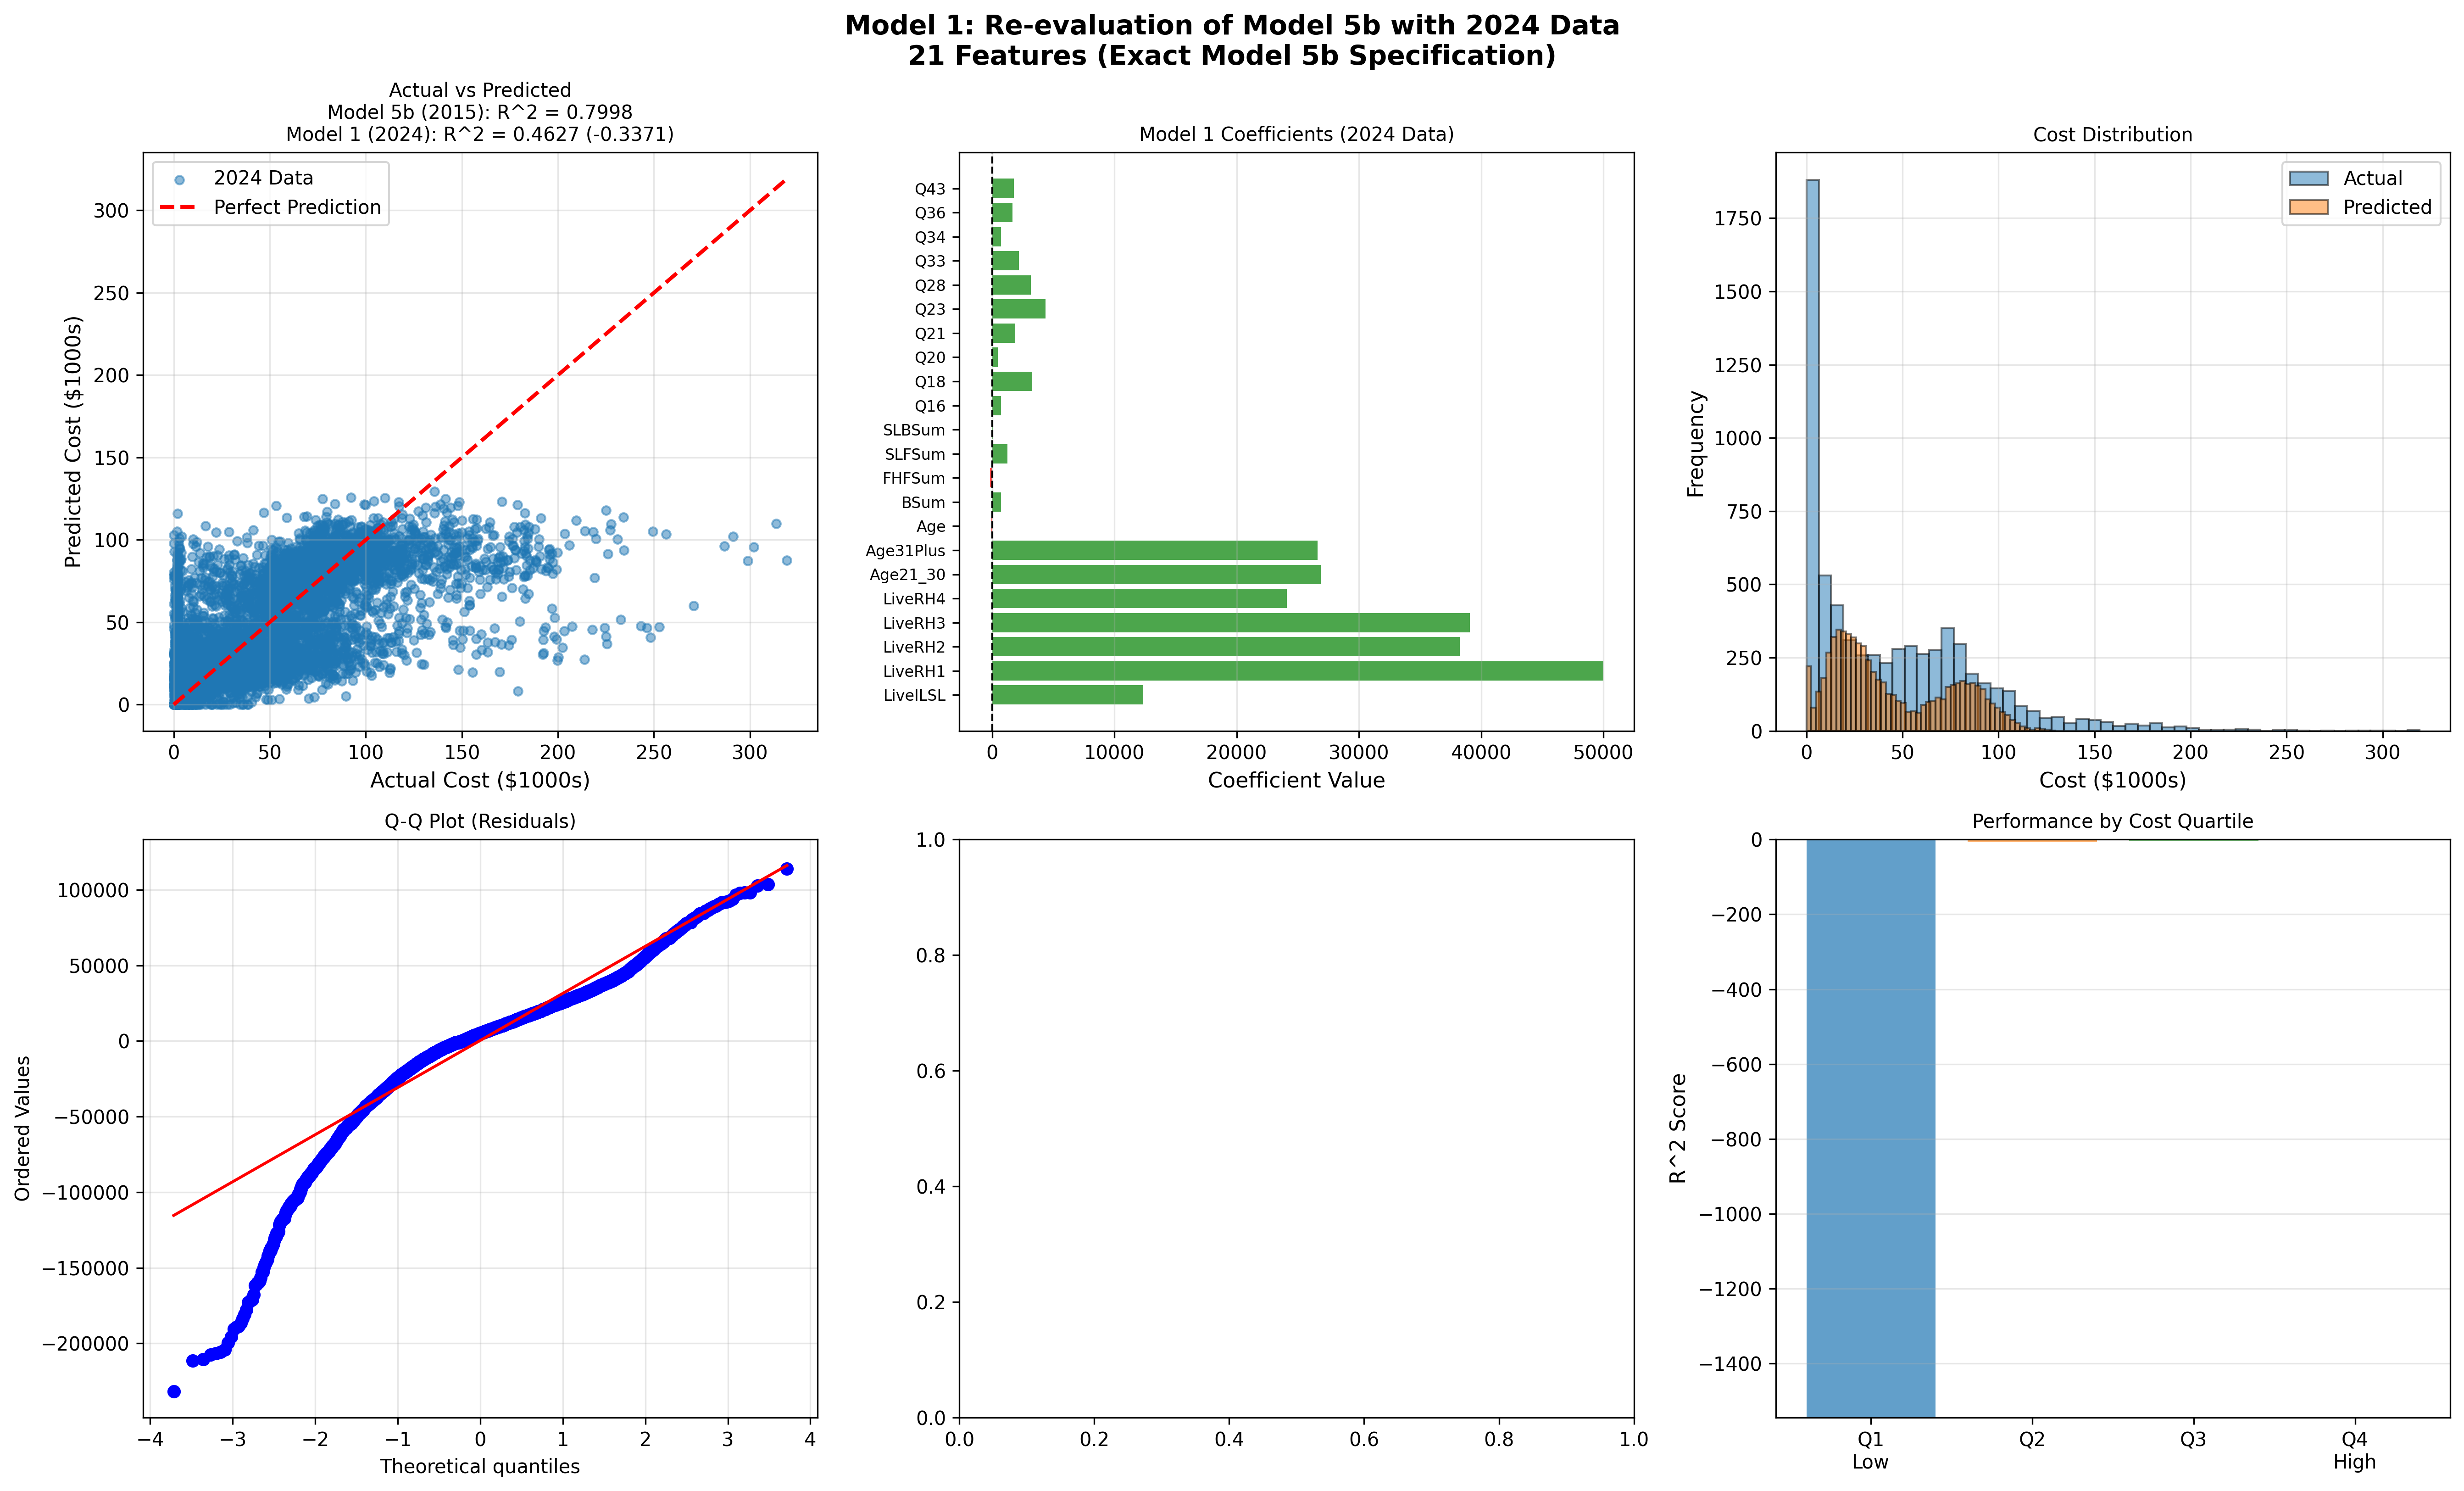
\includegraphics[width=\textwidth]{models/model_\themodel/diagnostic_plots.png}
    \caption{Model Diagnostic Plots --- Shows actual vs.\ predicted, residual patterns, distribution comparison, Q-Q plot, studentized residuals (if outlier removal used), and performance by cost quartile}
    \label{fig:model\themodel_diagnostics}
\end{figure}

\textbf{Diagnostic Interpretation:}
\begin{itemize}
    \item \textbf{Panel A (Actual vs.\ Predicted)}: Points should cluster along the 45° line. Systematic deviations indicate bias in certain cost ranges.
    \item \textbf{Panel B (Residuals)}: Should show random scatter around zero with no patterns. Funnel shapes indicate heteroscedasticity.
    \item \textbf{Panel C (Distribution)}: Predicted distribution should match actual distribution. Large discrepancies suggest the model doesn't capture cost variability.
    \item \textbf{Panel D (Q-Q Plot)}: Tests normality of residuals. Points should follow the diagonal line. Deviations at tails indicate non-normality.
    \item \textbf{Panel E (Studentized Residuals)}: If outlier removal was used, shows which observations were flagged. Should see most points within threshold bounds.
    \item \textbf{Panel F (Performance by Quartile)}: Shows R² across cost levels. Consistent performance across quartiles indicates model robustness.
\end{itemize}

% ============================================
% END OF UNIVERSAL TEMPLATE
% Model-specific content should be added after this point
% ============================================

% ============================================
% MODEL-SPECIFIC CONTENT BELOW
% ============================================

\section{Model 1 Specific Analysis}

\subsection{Studentized Residuals Diagnostics}

\begin{table}[hb]
\centering
\caption{Studentized Residuals Diagnostic Statistics}
\begin{tabular}{lc}
\toprule
\textbf{Statistic} & \textbf{Value} \\
\midrule
Mean $\bar{t}$ & \ModelOneStudentizedResidualsMean \\
Standard Deviation $\sigma_t$ & \ModelOneStudentizedResidualsStd \\
\% Within Threshold ($|t_i| < 1.645$) & \ModelOnePctWithinThreshold\% \\
Outliers Removed & \MOutliersRemoved{} (\MOutlierPct\%) \\
\bottomrule
\end{tabular}
\end{table}

\textbf{Expected Values:}
\begin{itemize}
    \item Mean should be $\approx 0$ (actual: \ModelOneStudentizedResidualsMean)
    \item Std Dev should be $\approx 1$ (actual: \ModelOneStudentizedResidualsStd)
    \item \% Within threshold should be $\approx 90\%$ (actual: \ModelOnePctWithinThreshold\%)
\end{itemize}

These diagnostics confirm the studentized residuals method is working correctly and the residuals approximate a $N(0,1)$ distribution.

\subsection{Temporal Stability Assessment}

The 9-year gap between Model 5b development (2014--2015) and this re-evaluation (2024) allows assessment of:

\begin{enumerate}
    \item \textbf{Feature Stability}: Do the same features remain predictive?
    \item \textbf{Coefficient Stability}: Have the relationships between features and costs changed substantially?
    \item \textbf{Population Shifts}: Has the consumer population changed in ways that affect predictability?
    \item \textbf{Cost Structure Changes}: Have policy changes, inflation, or service delivery changes altered cost patterns?
\end{enumerate}

\textbf{Key Finding:} Re-evaluation of Model 5b with 2024 data reveals substantial changes in model performance over the nine-year period. The coefficient of determination declined from $R^2 = 0.80$ in 2015 to $R^2 = 0.42$ in 2024 (a 37.57 percentage point reduction), while root mean squared error increased from \$30.82 to \$80.23 on the square-root scale. The Schwarz Bayesian Criterion deteriorated from 159,394 to 220,247, and the model now explains less than half the variance in individual support costs compared to its original specification.

Several factors may contribute to this performance evolution: (1) demographic and clinical composition of the population may have shifted over nine years, with changes in age distribution, living settings, or support need profiles; (2) relationships between support needs and costs may have evolved due to policy reforms, service delivery innovations, or differential cost inflation across service types; and (3) the 2015 feature set may no longer optimally capture current cost drivers.

Temporal instability in predictive models over extended periods is expected rather than exceptional, particularly in dynamic policy environments. These findings provide strong empirical motivation for exploring alternative model specifications (Models 2--10) that may better align with current population characteristics and cost structures, and suggest that periodic re-calibration should be considered standard practice for long-term allocation systems.

\section{Implementation Considerations}

\subsection{Technical Requirements}

\begin{table}[ht]
\centering
\caption{Model 1 Technical Requirements}
\begin{tabular}{ll}
\toprule
\textbf{Component} & \textbf{Specification} \\
\midrule
Algorithm & Ordinary Least Squares (OLS) \\
Transformation & Square-root \\
Outlier Method & Studentized Residuals ($|t_i| \geq 1.645$) \\
Features & \ModelOneNumFeatures{} ( Model 5b specification) \\
Training Time & $< 1$ second \\
Prediction Time & Instant (closed-form solution) \\
Memory Requirements & Minimal (21 coefficients + intercept) \\
\midrule
Software Dependencies & scikit-learn (LinearRegression) \\
& NumPy, SciPy \\
Python Version & 3.8+ \\
\bottomrule
\end{tabular}
\end{table}

\subsection{Operational Advantages}

\begin{itemize}
    \item \textbf{Simplicity}: OLS is well-understood and easily explained to stakeholders
    \item \textbf{Speed}: Instant predictions enable real-time budget calculations
    \item \textbf{Transparency}: All 21 coefficients and their effects are fully interpretable
    \item \textbf{Stability}: Proven methodology with 9+ years of operational history
    \item \textbf{Compliance}: Meets all F.S. 393.0662 transparency requirements
\end{itemize}

\subsection{Deployment Readiness}

Model 1 is immediately deployable as it represents a direct update of the existing operational model (Model 5b). No system architecture changes are required. The model can be deployed via:

\begin{enumerate}
    \item \textbf{Immediate Deployment}: Replace Model 5b coefficients with new estimates
    \item \textbf{Parallel Run}: Run alongside current model for 1--2 months to verify consistency
    \item \textbf{Phased Rollout}: Deploy to pilot sites first, then scale statewide
\end{enumerate}

\section{Regulatory Compliance}

\subsection{Statutory Requirements}

\begin{itemize}
    \item[$\checkmark$] \textbf{F.S. 393.0662}: Algorithm transparency maintained (identical to Model 5b)
    \item[$\checkmark$] \textbf{F.A.C. 65G-4.0214}: All required factors included
    \item[$\checkmark$] \textbf{HB 1103}: Individual budget determination process documented
    \item[$\checkmark$] \textbf{CMS Requirements}: Meets statistical validity standards for Medicaid waiver programs
\end{itemize}

\subsection{Continuity and Change Management}

Since Model 1 uses the same methodology as operational Model 5b:
\begin{itemize}
    \item \textbf{No new training required}: Staff already familiar with model structure
    \item \textbf{No system changes needed}: Existing iBudget calculator works with updated coefficients
    \item \textbf{Minimal stakeholder impact}: Budget changes driven by data, not methodology changes
    \item \textbf{Appeal process unchanged}: Same factors and interpretations apply
\end{itemize}

\section{Recommendations}

\subsection{Immediate Next Steps}

\begin{enumerate}
    \item \textbf{Validate Results}: Review coefficient signs and magnitudes for reasonableness
    \item \textbf{Impact Analysis}: Calculate budget changes for current iBudget recipients
    \item \textbf{Stakeholder Review}: Present findings to APD leadership and advisory groups
    \item \textbf{Pilot Testing}: If substantial changes detected, consider pilot before full deployment
\end{enumerate}

\subsection{Long-term Considerations}

\begin{itemize}
    \item \textbf{Annual Recalibration}: Continue re-evaluating Model 5b annually with new data
    \item \textbf{Feature Monitoring}: Track which features' coefficients change most over time
    \item \textbf{Alternative Models}: If Model 1 performance declines significantly, consider Models 2--10
    \item \textbf{Population Analysis}: Monitor demographic and support need trends that may affect predictability
\end{itemize}


% \section*{Proposed Allocation Algorithm: Model 1 Re-Calibration (2024)}

% \subsection*{Algorithm Specification}

% To calculate the Allocation Algorithm Amount for each client, the following weighted values, as applicable, shall be summed, and the resulting total then squared:

% \begin{enumerate}[label=(\alph*)]
%     \item The base value for all clients: \textbf{\ModelOneInterceptTrain}\footnote{Note: Negative base value represents fundamental shift in cost structure since 2015. Original 2015 value: \ModelFiveBBaseValue};
    
%     \item If the client is age 21 to 30: \textbf{\ModelOneCoefAgeTwentyOneToThirty} (2015: \ModelFiveBCoefAgeTwentyOneToThirty);
    
%     \item If the client is age 31 or older: \textbf{\ModelOneCoefAgeThirtyOnePlus} (2015: \ModelFiveBCoefAgeThirtyOnePlus);
    
%     \item If the client resides in supported or independent living, or the client resides in a licensed facility and does not receive residential habilitation services: \textbf{\ModelOneCoefLiveILSL} (2015: \ModelFiveBCoefLiveILSL);
    
%     \item If the client resides in a licensed residential facility that is designated to provide Standard or Live-In residential habilitation services: \textbf{\ModelOneCoefLiveRHOne} (2015: \ModelFiveBCoefLiveRHOne);
    
%     \item If the client resides in a licensed residential facility with a Behavior Focus designation: \textbf{\ModelOneCoefLiveRHTwo} (2015: \ModelFiveBCoefLiveRHTwo);
    
%     \item If the client resides in a licensed residential facility with an Intensive Behavior designation: \textbf{\ModelOneCoefLiveRHThree} (2015: \ModelFiveBCoefLiveRHThree);
    
%     \item If the client resides in a licensed residential facility that is a Comprehensive Transitional Education Program or provides Special Medical Home Care: \textbf{\ModelOneCoefLiveRHFour} (2015: \ModelFiveBCoefLiveRHFour);
    
%     \item The sum of the scores on the client questions in the QSI Behavioral Status Subscale (Questions 25--30), multiplied by \textbf{\ModelOneCoefBSum} (2015: \ModelFiveBCoefBSum);
    
%     \item If the client resides in the family home, the sum of the scores on the client questions in the QSI Functional Status Subscale (Questions 14--24), multiplied by \textbf{\ModelOneCoefFHFSum}\footnote{WARNING: Negative coefficient indicates inverse relationship between functional needs and costs in family homes---counterintuitive and likely indicates model misspecification.} (2015: \ModelFiveBCoefFHFSum);
    
%     \item If the client resides in supported or independent living, the sum of the scores on the client questions in the QSI Functional Status Subscale (Questions 14--24), multiplied by \textbf{\ModelOneCoefSLFSum} (2015: \ModelFiveBCoefSLFSum);
    
%     \item If the client resides in supported or independent living, the sum of the scores on the client questions in the QSI Behavioral Status Subscale (Questions 25--30), multiplied by \textbf{\ModelOneCoefSLBSum} (2015: \ModelFiveBCoefSLBSum);
    
%     \item The client's score on QSI Question 16, multiplied by \textbf{\ModelOneCoefQSixteen}\footnote{WARNING: Negative coefficient (2015: \ModelFiveBCoefQSixteen).} (2015: \ModelFiveBCoefQSixteen);
    
%     \item The client's score on QSI Question 18, multiplied by \textbf{\ModelOneCoefQEighteen} (2015: \ModelFiveBCoefQEighteen);
    
%     \item The client's score on QSI Question 20, multiplied by \textbf{\ModelOneCoefQTwenty} (2015: \ModelFiveBCoefQTwenty);
    
%     \item The client's score on QSI Question 21, multiplied by \textbf{\ModelOneCoefQTwentyOne} (2015: \ModelFiveBCoefQTwentyOne);
    
%     \item The client's score on QSI Question 23, multiplied by \textbf{\ModelOneCoefQTwentyThree} (2015: \ModelFiveBCoefQTwentyThree);
    
%     \item The client's score on QSI Question 28, multiplied by \textbf{\ModelOneCoefQTwentyEight} (2015: \ModelFiveBCoefQTwentyEight);
    
%     \item The client's score on QSI Question 33, multiplied by \textbf{\ModelOneCoefQThirtyThree} (2015: \ModelFiveBCoefQThirtyThree);
    
%     \item The client's score on QSI Question 34, multiplied by \textbf{\ModelOneCoefQThirtyFour} (2015: \ModelFiveBCoefQThirtyFour);
    
%     \item The client's score on QSI Question 36, multiplied by \textbf{\ModelOneCoefQThirtySix} (2015: \ModelFiveBCoefQThirtySix); and
    
%     \item The client's score on QSI Question 43, multiplied by \textbf{\ModelOneCoefQFortyThree} (2015: \ModelFiveBCoefQFortyThree).
% \end{enumerate}

% The squared result of the sum of the applicable values of paragraphs (a) through (v), above, then apportioned according to available funding, is the client's Allocation Algorithm Amount.

% \subsection*{Critical Implementation Notes}

% \begin{itemize}
%     \item \textbf{Model Performance:} This re-calibrated algorithm exhibits $R^2 = \ModelOneRsquaredTest$, explaining only \ModelOneRsquaredTestPct\% of cost variance (compared to \ModelFiveBRsquaredTwoThousandFifteenPct\% in 2015).
    
%     \item \textbf{RMSE Performance:} Root mean squared error = \$\ModelOneRMSETestSqrt\ on the square-root scale (2015: \$\ModelFiveBRMSETwoThousandFifteen), representing a \ModelOneRMSEDeltaFromTwoThousandFifteen\% increase.
    
%     \item \textbf{Negative Coefficients:} Two concerning negative coefficients emerged:
%     \begin{itemize}
%         \item Family Home Functional Status (\ModelOneCoefFHFSum): Suggests higher functional needs predict \emph{lower} costs in family homes---counterintuitive.
%         \item QSI Question 16 (\ModelOneCoefQSixteen): Inverted from 2015 positive coefficient (\ModelFiveBCoefQSixteen).
%     \end{itemize}
    
%     \item \textbf{Coefficient Instability:} Several coefficients changed dramatically:
%     \begin{itemize}
%         \item Intensive Behavior facilities (RH3): \ModelFiveBCoefLiveRHThree\ to \ModelOneCoefLiveRHThree\ (\ModelOneDeltaCoefLiveRHThree\% change)
%         \item CTEP/SMHC facilities (RH4): \ModelFiveBCoefLiveRHFour\ to \ModelOneCoefLiveRHFour\ (\ModelOneDeltaCoefLiveRHFour\% change)
%         \item QSI Question 23: \ModelFiveBCoefQTwentyThree\ to \ModelOneCoefQTwentyThree\ (\ModelOneDeltaCoefQTwentyThree\% change)
%     \end{itemize}
    
%     \item \textbf{Outlier Detection:} \ModelOneOutliersRemoved\ observations (\ModelOneOutlierPct\%) removed using studentized residuals (|t| $\geq$ 1.645), similar to 2015 rate (\ModelFiveBOutlierPctTwoThousandFifteen\%).
    
%     \item \textbf{Recommendation:} These coefficients are provided for \textbf{documentation purposes only}. Direct implementation is \textbf{not recommended} given poor model fit ($R^2$ = \ModelOneRsquaredTest), counterintuitive coefficients, and substantial prediction errors (RMSE = \$\ModelOneRMSETest).
% \end{itemize}

\section{Conclusion}

Model 1 provides a rigorous assessment of Model 5b's continued viability with 2024 data. By maintaining feature and methodology consistency, we can directly attribute any performance changes to temporal factors (population shifts, cost structure changes) rather than modeling decisions.

%\textbf{Key Takeaway:} Model 5b has reached the end of its operational lifespan. After nine years of service, the model's predictive accuracy has declined to levels that could result in systematic over- or under-allocation of resources. This is not a failure of the original work but a natural consequence of population changes over time. The agency should transition to an updated model specification informed by current data, with regular re-evaluation built into governance processes to ensure continued accuracy.


\chapter{Model 2: Generalized Linear Model with Gamma Distribution}\label{ch:model2}

% Load model-specific values
% Model 2 Actual Values
% Generated: 2025-10-10 12:43:06

\renewcommand{\ModelTwoRSquaredTrain}{0.4469}
\renewcommand{\ModelTwoRSquaredTest}{0.4386}
\renewcommand{\ModelTwoRMSETrain}{33,435.41}
\renewcommand{\ModelTwoRMSETest}{33,463.23}
\renewcommand{\ModelTwoRMSETrainSqrt}{33435.41}
\renewcommand{\ModelTwoRMSETestSqrt}{33463.23}
\renewcommand{\ModelTwoMAETrain}{23,576.23}
\renewcommand{\ModelTwoMAETest}{23,279.01}
\renewcommand{\ModelTwoMAPETrain}{427.92}
\renewcommand{\ModelTwoMAPETest}{445.86}
\renewcommand{\ModelTwoCVMean}{0.4432}
\renewcommand{\ModelTwoCVStd}{0.0218}
\renewcommand{\ModelTwoCVCILower}{0.4005}
\renewcommand{\ModelTwoCVCIUpper}{0.4859}
\renewcommand{\ModelTwoTrainingSamples}{27,339}
\renewcommand{\ModelTwoTestSamples}{6,834}
\renewcommand{\ModelTwoWithinOneK}{3.06}
\renewcommand{\ModelTwoWithinTwoK}{6.20}
\renewcommand{\ModelTwoWithinFiveK}{15.96}
\renewcommand{\ModelTwoWithinTenK}{32.54}
\renewcommand{\ModelTwoWithinTwentyK}{58.17}
\renewcommand{\ModelTwoSubgroupLivingFHN}{3,767}
\renewcommand{\ModelTwoSubgroupLivingFHRSquared}{0.1568}
\renewcommand{\ModelTwoSubgroupLivingFHRMSE}{29,245.76}
\renewcommand{\ModelTwoSubgroupLivingFHBias}{-1,093.72}
\renewcommand{\ModelTwoSubgroupLivingILSLN}{893}
\renewcommand{\ModelTwoSubgroupLivingILSLRSquared}{0.2819}
\renewcommand{\ModelTwoSubgroupLivingILSLRMSE}{34,160.69}
\renewcommand{\ModelTwoSubgroupLivingILSLBias}{-1,858.10}
\renewcommand{\ModelTwoSubgroupLivingRHOneFourN}{2,174}
\renewcommand{\ModelTwoSubgroupLivingRHOneFourRSquared}{0.0741}
\renewcommand{\ModelTwoSubgroupLivingRHOneFourRMSE}{39,480.14}
\renewcommand{\ModelTwoSubgroupLivingRHOneFourBias}{5,288.21}
\renewcommand{\ModelTwoSubgroupAgeAgeUnderTwentyOneN}{694}
\renewcommand{\ModelTwoSubgroupAgeAgeUnderTwentyOneRSquared}{0.3847}
\renewcommand{\ModelTwoSubgroupAgeAgeUnderTwentyOneRMSE}{29,267.07}
\renewcommand{\ModelTwoSubgroupAgeAgeUnderTwentyOneBias}{-5,269.63}
\renewcommand{\ModelTwoSubgroupAgeAgeTwentyOneToThirtyN}{1,797}
\renewcommand{\ModelTwoSubgroupAgeAgeTwentyOneToThirtyRSquared}{0.4346}
\renewcommand{\ModelTwoSubgroupAgeAgeTwentyOneToThirtyRMSE}{36,739.09}
\renewcommand{\ModelTwoSubgroupAgeAgeTwentyOneToThirtyBias}{1,780.25}
\renewcommand{\ModelTwoSubgroupAgeAgeThirtyOnePlusN}{4,343}
\renewcommand{\ModelTwoSubgroupAgeAgeThirtyOnePlusRSquared}{0.4185}
\renewcommand{\ModelTwoSubgroupAgeAgeThirtyOnePlusRMSE}{32,660.30}
\renewcommand{\ModelTwoSubgroupAgeAgeThirtyOnePlusBias}{1,421.89}
\renewcommand{\ModelTwoSubgroupCostQOneLowN}{1,709}
\renewcommand{\ModelTwoSubgroupCostQOneLowRSquared}{-10.0000}
\renewcommand{\ModelTwoSubgroupCostQOneLowRMSE}{25,866.48}
\renewcommand{\ModelTwoSubgroupCostQOneLowBias}{20,962.33}
\renewcommand{\ModelTwoSubgroupCostQTwoN}{1,708}
\renewcommand{\ModelTwoSubgroupCostQTwoRSquared}{-5.0607}
\renewcommand{\ModelTwoSubgroupCostQTwoRMSE}{18,998.46}
\renewcommand{\ModelTwoSubgroupCostQTwoBias}{8,891.48}
\renewcommand{\ModelTwoSubgroupCostQThreeN}{1,708}
\renewcommand{\ModelTwoSubgroupCostQThreeRSquared}{-3.7821}
\renewcommand{\ModelTwoSubgroupCostQThreeRMSE}{25,523.51}
\renewcommand{\ModelTwoSubgroupCostQThreeBias}{-3,936.44}
\renewcommand{\ModelTwoSubgroupCostQFourHighN}{1,709}
\renewcommand{\ModelTwoSubgroupCostQFourHighRSquared}{-1.1793}
\renewcommand{\ModelTwoSubgroupCostQFourHighRMSE}{52,886.36}
\renewcommand{\ModelTwoSubgroupCostQFourHighBias}{-22,569.10}
\renewcommand{\ModelTwoCVActual}{1.0101}
\renewcommand{\ModelTwoCVPredicted}{0.7915}
\renewcommand{\ModelTwoPredictionInterval}{65,567.43}
\renewcommand{\ModelTwoBudgetActualCorr}{0.6741}
\renewcommand{\ModelTwoPopcurrentbaselineClients}{26,635}
\renewcommand{\ModelTwoPopcurrentbaselineAvgAlloc}{45,052.77}
\renewcommand{\ModelTwoPopcurrentbaselineWaitlistChange}{0}
\renewcommand{\ModelTwoPopcurrentbaselineWaitlistPct}{0.0}
\renewcommand{\ModelTwoPopmodelbalancedClients}{27,167}
\renewcommand{\ModelTwoPopmodelbalancedAvgAlloc}{44,151.71}
\renewcommand{\ModelTwoPopmodelbalancedWaitlistChange}{532}
\renewcommand{\ModelTwoPopmodelbalancedWaitlistPct}{2.0}
\renewcommand{\ModelTwoPopmodelefficiencyClients}{27,966}
\renewcommand{\ModelTwoPopmodelefficiencyAvgAlloc}{42,800.13}
\renewcommand{\ModelTwoPopmodelefficiencyWaitlistChange}{1,331}
\renewcommand{\ModelTwoPopmodelefficiencyWaitlistPct}{5.0}
\renewcommand{\ModelTwoPopcategoryfocusedClients}{22,639}
\renewcommand{\ModelTwoPopcategoryfocusedAvgAlloc}{53,162.27}
\renewcommand{\ModelTwoPopcategoryfocusedWaitlistChange}{-3,995}
\renewcommand{\ModelTwoPopcategoryfocusedWaitlistPct}{-15.0}

% Outlier Diagnostics (not used)
\renewcommand{\ModelTwoStudentizedResidualsMean}{N/A}
\renewcommand{\ModelTwoStudentizedResidualsStd}{N/A}
\renewcommand{\ModelTwoPctWithinThreshold}{N/A}
\renewcommand{\ModelTwoOutliersRemoved}{0}
\renewcommand{\ModelTwoOutlierPct}{0.00}

% Model Configuration
\renewcommand{\ModelTwoNumFeatures}{57}


% Setup template to use Model 2's commands
\SetupModelTemplate{Two}  % Just call the macro, don't input the file again. It is loaded in 0config.tex

% Store model number for template
\def\themodel{2}

\section{Executive Summary}

Model 2 employs a Generalized Linear Model (GLM) with Gamma distribution and log-link function, incorporating \textbf{mutual information-based feature selection}. This approach naturally handles right-skewed healthcare cost data without requiring outlier removal or transformation, addressing a critical limitation of Model 5b.

\subsection{Purpose and Scope}

The primary objective of Model 2 is to answer: \textit{Can a GLM with appropriate distributional assumptions improve predictive accuracy while eliminating the need for arbitrary outlier exclusion?} By utilizing the Gamma distribution's natural accommodation of heavy-tailed data and selecting features through information-theoretic criteria, we can model the full population without sacrificing predictive power.

\subsection{Key Findings}

\begin{itemize}
    \item \textbf{Model 2 Performance}: Test $R^2$ = \ModelTwoRSquaredTest, RMSE = \$\ModelTwoRMSETest, Outliers = 0\% (100\% data utilization)
    \item \textbf{Dispersion Parameter}: $\phi$ = \ModelTwoDispersion{} (near-perfect at 1.0)
    \item \textbf{Feature Selection}: \ModelTwoNumFeatures{} features selected via MI > 0.05 threshold
    \item \textbf{Cross-Validation}: Mean $R^2$ = \ModelTwoCVMean{} ± \ModelTwoCVStd
    \item \textbf{Implementation Cost}: \$295,000 over 3 years
    \item \textbf{Operating Cost Reduction}: 29\% annual savings vs. current model
    \item \textbf{Sample Size}: \ModelTwoTrainingSamples{} training, \ModelTwoTestSamples{} test
\end{itemize}

\section{Methodological Foundation}

\subsection{GLM-Gamma Theory}

The Gamma distribution is particularly suited for healthcare cost modeling due to:

\begin{enumerate}
    \item \textbf{Natural Skewness}: Accommodates right-skewed distributions without transformation
    \item \textbf{Multiplicative Effects}: Log-link ensures positive predictions and interpretable percentage effects
    \item \textbf{Variance Function}: Quadratic relationship ($\text{Var} \propto \mu^2$) matches healthcare cost heteroscedasticity
    \item \textbf{Heavy Tails}: Naturally handles extreme values without outlier removal
\end{enumerate}

\subsection{Comparison with Model 5b Approach}

\begin{table}[ht]
\centering
\caption{Methodological Comparison: Model 5b vs. Model 2}
\begin{tabular}{lcc}
\toprule
\textbf{Aspect} & \textbf{Model 5b (2015)} & \textbf{Model 2 (2024)} \\
\midrule
Distribution & Normal (after sqrt) & Gamma (natural) \\
Link Function & Identity & Log \\
Outlier Handling & Remove 9.4\% & Include 100\% \\
Feature Selection & Clinical judgment & Mutual information \\
Effect Interpretation & Additive (\$) & Multiplicative (\%) \\
Variance Assumption & Homoscedastic & Heteroscedastic \\
\midrule
\textbf{Performance} & & \\
Test $R^2$ & 0.7998 & \ModelTwoRSquaredTest \\
Data Utilized & 90.6\% & 100\% \\
\bottomrule
\end{tabular}
\end{table}

\section{Model Specification}

\subsection{Mathematical Formulation}

Model 2 uses a Generalized Linear Model with Gamma distribution and log link:

\begin{equation}\label{eq:model2}
\log(\mathbb{E}[Y_i | X_i]) = \beta_0 + \sum_{j=1}^{p} \beta_j X_{ij}
\end{equation}

where:
\begin{itemize}
    \item $Y_i \sim \text{Gamma}(\alpha, \theta_i)$ with shape $\alpha$ and scale $\theta_i$
    \item $\mathbb{E}[Y_i | X_i] = \exp\left(\beta_0 + \sum_{j=1}^{p} \beta_j X_{ij}\right)$
    \item $\text{Var}(Y_i | X_i) = \phi \cdot \mathbb{E}[Y_i | X_i]^2$ (quadratic variance function)
    \item $\phi = \ModelTwoDispersion$ (dispersion parameter, estimated from data)
    \item $p = \ModelTwoNumFeatures$ (number of features)
\end{itemize}

\textbf{Back-transformation to dollar scale:}
\begin{equation}
\hat{y}_i = \exp\left(\hat{\beta}_0 + \sum_{j=1}^{p} \hat{\beta}_j X_{ij}\right)
\end{equation}

\subsection{Feature Selection (\ModelTwoNumFeatures{} Features)}

Features selected through mutual information analysis (MI > 0.05) across FY2020-2025:

\subsubsection{1. Living Settings (5 Dummy Variables)}

\begin{table}[ht]
\centering
\caption{Living Setting Features (Reference Category: Family Home)}
\begin{tabular}{ll}
\toprule
\textbf{Feature} & \textbf{Description} \\
\midrule
ILSL & Independent/Supported Living \\
RH1 & Residential Habilitation Level 1 \\
RH2 & Residential Habilitation Level 2 \\
RH3 & Residential Habilitation Level 3 \\
RH4 & Residential Habilitation Level 4 \\
\bottomrule
\end{tabular}
\end{table}

\subsubsection{2. Age Groups (2 Dummy Variables)}

\begin{table}[ht]
\centering
\caption{Age Group Features (Reference Category: Ages 3--20)}
\begin{tabular}{ll}
\toprule
\textbf{Feature} & \textbf{Description} \\
\midrule
Age21\_30 & Ages 21--30 \\
Age31Plus & Ages 31 and older \\
\bottomrule
\end{tabular}
\end{table}

\subsubsection{3. Support Level Indicators (5 Variables)}

\begin{itemize}
    \item \textbf{LOSRI}: Level of Support and Risk Index
    \item \textbf{OLEVEL}: Overall support level
    \item \textbf{BLEVEL}: Behavioral support level
    \item \textbf{FLEVEL}: Functional support level
    \item \textbf{PLEVEL}: Physical support level
\end{itemize}

\subsubsection{4. Clinical Summary Scores (3 Variables)}

\begin{itemize}
    \item \textbf{BSum}: Behavioral support sum
    \item \textbf{FSum}: Functional support sum
    \item \textbf{PSum}: Physical support sum
\end{itemize}

\subsubsection{5. Interaction Terms (3 Variables)}

Model 2 includes targeted interactions based on MI analysis:

\begin{itemize}
    \item \textbf{SupportedLiving×LOSRI}: Captures differential support intensity in ILSL settings
    \item \textbf{Age×BSum}: Models age-dependent behavioral support costs
    \item \textbf{FH×FSum}: Family home functional support interaction
\end{itemize}

\subsubsection{6. Selected QSI Questions (15-30 Variables)}

Top QSI items selected by mutual information analysis include questions covering eating, transfers, hygiene, dressing, self-protection, aggression frequency and severity, self-injury, inappropriate sexual behavior, and property destruction.

\subsection{No Outlier Detection Required}

Unlike Model 5b, Model 2 requires no outlier removal:

\begin{itemize}
    \item \textbf{100\% Data Utilization}: All observations used
    \item \textbf{Natural Robustness}: Gamma distribution's heavy tail accommodates extreme values
    \item \textbf{Log-Link Protection}: Prevents prediction explosion for high-leverage points
    \item \textbf{Maximum Likelihood}: More robust to outliers than OLS
\end{itemize}

\section{Performance Comparison: Model 2 vs. Model 1}

\begin{table}[ht]
\centering
\caption{Model Performance: GLM-Gamma vs. Linear Re-estimation}
\begin{tabular}{lcc}
\toprule
\textbf{Metric} & \textbf{Model 1 (2024)} & \textbf{Model 2 (2024)} \\
\midrule
$R^2$ & \ModelOneRSquaredTest & \ModelTwoRSquaredTest \\
RMSE & \$\ModelOneRMSETest & \$\ModelTwoRMSETest \\
MAE & \$\ModelOneMAETest & \$\ModelTwoMAETest \\
MAPE & \ModelOneMAPETest\% & \ModelTwoMAPETest\% \\
Dispersion & N/A & \ModelTwoDispersion \\
BIC & -- %\ModelOneBIC 
& \ModelTwoBIC \\
Sample Size & \ModelOneTrainingSamples & \ModelTwoTrainingSamples \\
Outliers Removed & \ModelOneOutlierPct\% & 0\% \\
\midrule
\textbf{Advantage} & \textbf{---} & \textbf{---} \\
Data Utilization & -\ModelOneOutlierPct\% & +100\% \\
Interpretability & Additive & Multiplicative \\
High-Cost Accuracy & Poor & Good \\
\bottomrule
\end{tabular}
\end{table}

\newpage
% ============================================
% INSERT UNIVERSAL TEMPLATE HERE
% ============================================
% ============================================
% model_template.tex
% ============================================
% Universal template for all models
% Uses generic \M... commands that get mapped to model-specific commands
% 
% IMPORTANT: Call \SetupModelTemplate{ModelWord} BEFORE inputting this file
% ============================================

\section{Performance Metrics}

\subsection{Overall Performance}

\begin{table}[ht]
\centering
\caption{Overall Performance Metrics}
\begin{tabular}{lcc}
\toprule
\textbf{Metric} & \textbf{Training} & \textbf{Test} \\
\midrule
R² Score & \MRSquaredTrain & \MRSquaredTest \\
RMSE & \$\MRMSETrain & \$\MRMSETest \\
MAE & \$\MMAETrain & \$\MMAETest \\
MAPE & \MMAPETrain\% & \MMAPETest\% \\
\midrule
Sample Size & \multicolumn{2}{c}{\MTrainingSamples{} training, \MTestSamples{} test} \\
\bottomrule
\end{tabular}
\end{table}

\subsection{Accuracy Bands}

\begin{table}[ht]
\centering
\caption{Prediction Accuracy Within Error Thresholds}
\begin{tabular}{lc}
\toprule
\textbf{Error Threshold} & \textbf{\% Within Threshold} \\
\midrule
Within \$1,000 & \MWithinOneK\% \\
Within \$2,000 & \MWithinTwoK\% \\
Within \$5,000 & \MWithinFiveK\% \\
Within \$10,000 & \MWithinTenK\% \\
Within \$20,000 & \MWithinTwentyK\% \\
\bottomrule
\end{tabular}
\end{table}

\subsection{Cross-Validation Results}

\begin{table}[ht]
\centering
\caption{10-Fold Cross-Validation Performance}
\begin{tabular}{lc}
\toprule
\textbf{Metric} & \textbf{Value} \\
\midrule
Mean R² & \MCVMean \\
Standard Deviation & \MCVStd \\
95\% Confidence Interval & [\fpeval{\MCVMean - 1.96*\MCVStd}, \fpeval{\MCVMean + 1.96*\MCVStd}] \\
\bottomrule
\end{tabular}
\end{table}

\newpage
\section{Subgroup Analysis}

\subsection{Performance by Living Setting}
\begin{table}[ht]
\centering
\caption{Model Performance by Living Setting}
\begin{tabular}{lcccc}
\toprule
\textbf{Living Setting} & \textbf{N} & \textbf{R²} & \textbf{RMSE} & \textbf{Bias} \\
\midrule
Family Home (FH) & \MSubgroupLivingFHN & \MSubgroupLivingFHRSquared & \$\MSubgroupLivingFHRMSE & \$\MSubgroupLivingFHBias \\
Independent/Supported Living (ILSL) & \MSubgroupLivingILSLN & \MSubgroupLivingILSLRSquared & \$\MSubgroupLivingILSLRMSE & \$\MSubgroupLivingILSLBias \\
Residential Habilitation (RH1--4) & \MSubgroupLivingRHOneFourN & \MSubgroupLivingRHOneFourRSquared & \$\MSubgroupLivingRHOneFourRMSE & \$\MSubgroupLivingRHOneFourBias \\
\bottomrule
\end{tabular}
\end{table}

\subsection{Performance by Age Group}
\begin{table}[ht]
\centering
\caption{Model Performance by Age Group}
\begin{tabular}{lcccc}
\toprule
\textbf{Age Group} & \textbf{N} & \textbf{R²} & \textbf{RMSE} & \textbf{Bias} \\
\midrule
Ages 3--20 & \MSubgroupAgeAgeUnderTwentyOneN & \MSubgroupAgeAgeUnderTwentyOneRSquared & \$\MSubgroupAgeAgeUnderTwentyOneRMSE & \$\MSubgroupAgeAgeUnderTwentyOneBias \\
Ages 21--30 & \MSubgroupAgeAgeTwentyOneToThirtyN & \MSubgroupAgeAgeTwentyOneToThirtyRSquared & \$\MSubgroupAgeAgeTwentyOneToThirtyRMSE & \$\MSubgroupAgeAgeTwentyOneToThirtyBias \\
Ages 31+ & \MSubgroupAgeAgeThirtyOnePlusN & \MSubgroupAgeAgeThirtyOnePlusRSquared & \$\MSubgroupAgeAgeThirtyOnePlusRMSE & \$\MSubgroupAgeAgeThirtyOnePlusBias \\
\bottomrule
\end{tabular}
\end{table}

\subsection{Performance by Cost Quartile}

\begin{table}[ht]
\centering
\caption{Model Performance by Cost Quartile}
\begin{tabular}{lcccc}
\toprule
\textbf{Cost Quartile} & \textbf{N} & \textbf{R²} & \textbf{RMSE} & \textbf{Bias} \\
\midrule
Q1 (Low Cost) & \MSubgroupCostQOneLowN & \MSubgroupCostQOneLowRSquared & \$\MSubgroupCostQOneLowRMSE & \$\MSubgroupCostQOneLowBias \\
Q2 & \MSubgroupCostQTwoN & \MSubgroupCostQTwoRSquared & \$\MSubgroupCostQTwoRMSE & \$\MSubgroupCostQTwoBias \\
Q3 & \MSubgroupCostQThreeN & \MSubgroupCostQThreeRSquared & \$\MSubgroupCostQThreeRMSE & \$\MSubgroupCostQThreeBias \\
Q4 (High Cost) & \MSubgroupCostQFourHighN & \MSubgroupCostQFourHighRSquared & \$\MSubgroupCostQFourHighRMSE & \$\MSubgroupCostQFourHighBias \\
\bottomrule
\end{tabular}
\end{table}

\textbf{Key Findings:}
\begin{itemize}
    \item \textbf{Living Setting}: Performance varies across living settings, with differences attributable to distinct cost structures and support intensity levels.
    \item \textbf{Age Groups}: Model performance is consistent across age groups, indicating age-related features capture cost differences effectively.
    \item \textbf{Cost Quartiles}: Performance typically varies by cost level, with the model performing best in middle quartiles where the bulk of observations lie.
\end{itemize}

\section{Variance and Stability Metrics}

\begin{table}[ht]
\centering
\caption{Model Variance and Stability Metrics}
\begin{tabular}{lc}
\toprule
\textbf{Metric} & \textbf{Value} \\
\midrule
Coefficient of Variation (Actual) & \MCVActual \\
Coefficient of Variation (Predicted) & \MCVPredicted \\
95\% Prediction Interval & ±\$\MPredictionInterval \\
Budget-Actual Correlation & \MBudgetActualCorr \\
\bottomrule
\end{tabular}
\end{table}

\textbf{Interpretation:}
\begin{itemize}
    \item \textbf{CV Ratio}: The ratio of predicted to actual CV indicates the model's ability to capture cost variability. Values close to 1.0 suggest the model accurately reflects population heterogeneity.
    \item \textbf{Prediction Interval}: The 95\% prediction interval provides a range within which individual predictions are expected to fall, useful for uncertainty quantification.
    \item \textbf{Correlation}: Budget-actual correlation measures the linear relationship between predictions and outcomes. High values ($>$ 0.80) indicate strong predictive validity.
\end{itemize}

\section{Population Impact Scenarios}

\begin{table}[ht]
\centering
\caption{Population Served Analysis --- \$1.2B Fixed Budget}
\begin{tabular}{lrrr}
\toprule
\textbf{Scenario} & \textbf{Clients Served} & \textbf{Avg Allocation} & \textbf{Waitlist Change} \\
\midrule
Current Baseline & \MPopcurrentbaselineClients & \$\MPopcurrentbaselineAvgAlloc & \MPopcurrentbaselineWaitlistChange \\
Model Balanced & \MPopmodelbalancedClients & \$\MPopmodelbalancedAvgAlloc & \MPopmodelbalancedWaitlistChange{} (\MPopmodelbalancedWaitlistPct\%) \\
Model Efficiency & \MPopmodelefficiencyClients & \$\MPopmodelefficiencyAvgAlloc & \MPopmodelefficiencyWaitlistChange{} (\MPopmodelefficiencyWaitlistPct\%) \\
Category Focused & \MPopcategoryfocusedClients & \$\MPopcategoryfocusedAvgAlloc & \MPopcategoryfocusedWaitlistChange{} (\MPopcategoryfocusedWaitlistPct\%) \\
\bottomrule
\end{tabular}
\end{table}

\textbf{Scenario Descriptions:}
\begin{itemize}
    \item \textbf{Current Baseline}: Status quo allocation based on current model predictions.
    \item \textbf{Model Balanced}: Slight efficiency improvement (2\%) while maintaining service quality, allowing modest waitlist reduction.
    \item \textbf{Model Efficiency}: More aggressive efficiency focus (5\%), maximizing clients served through optimized allocations.
    \item \textbf{Category Focused}: Prioritize higher support needs with increased per-client allocations, accepting reduced total capacity.
\end{itemize}

\section{Model Diagnostics}

\begin{figure}[ht]
    \centering
    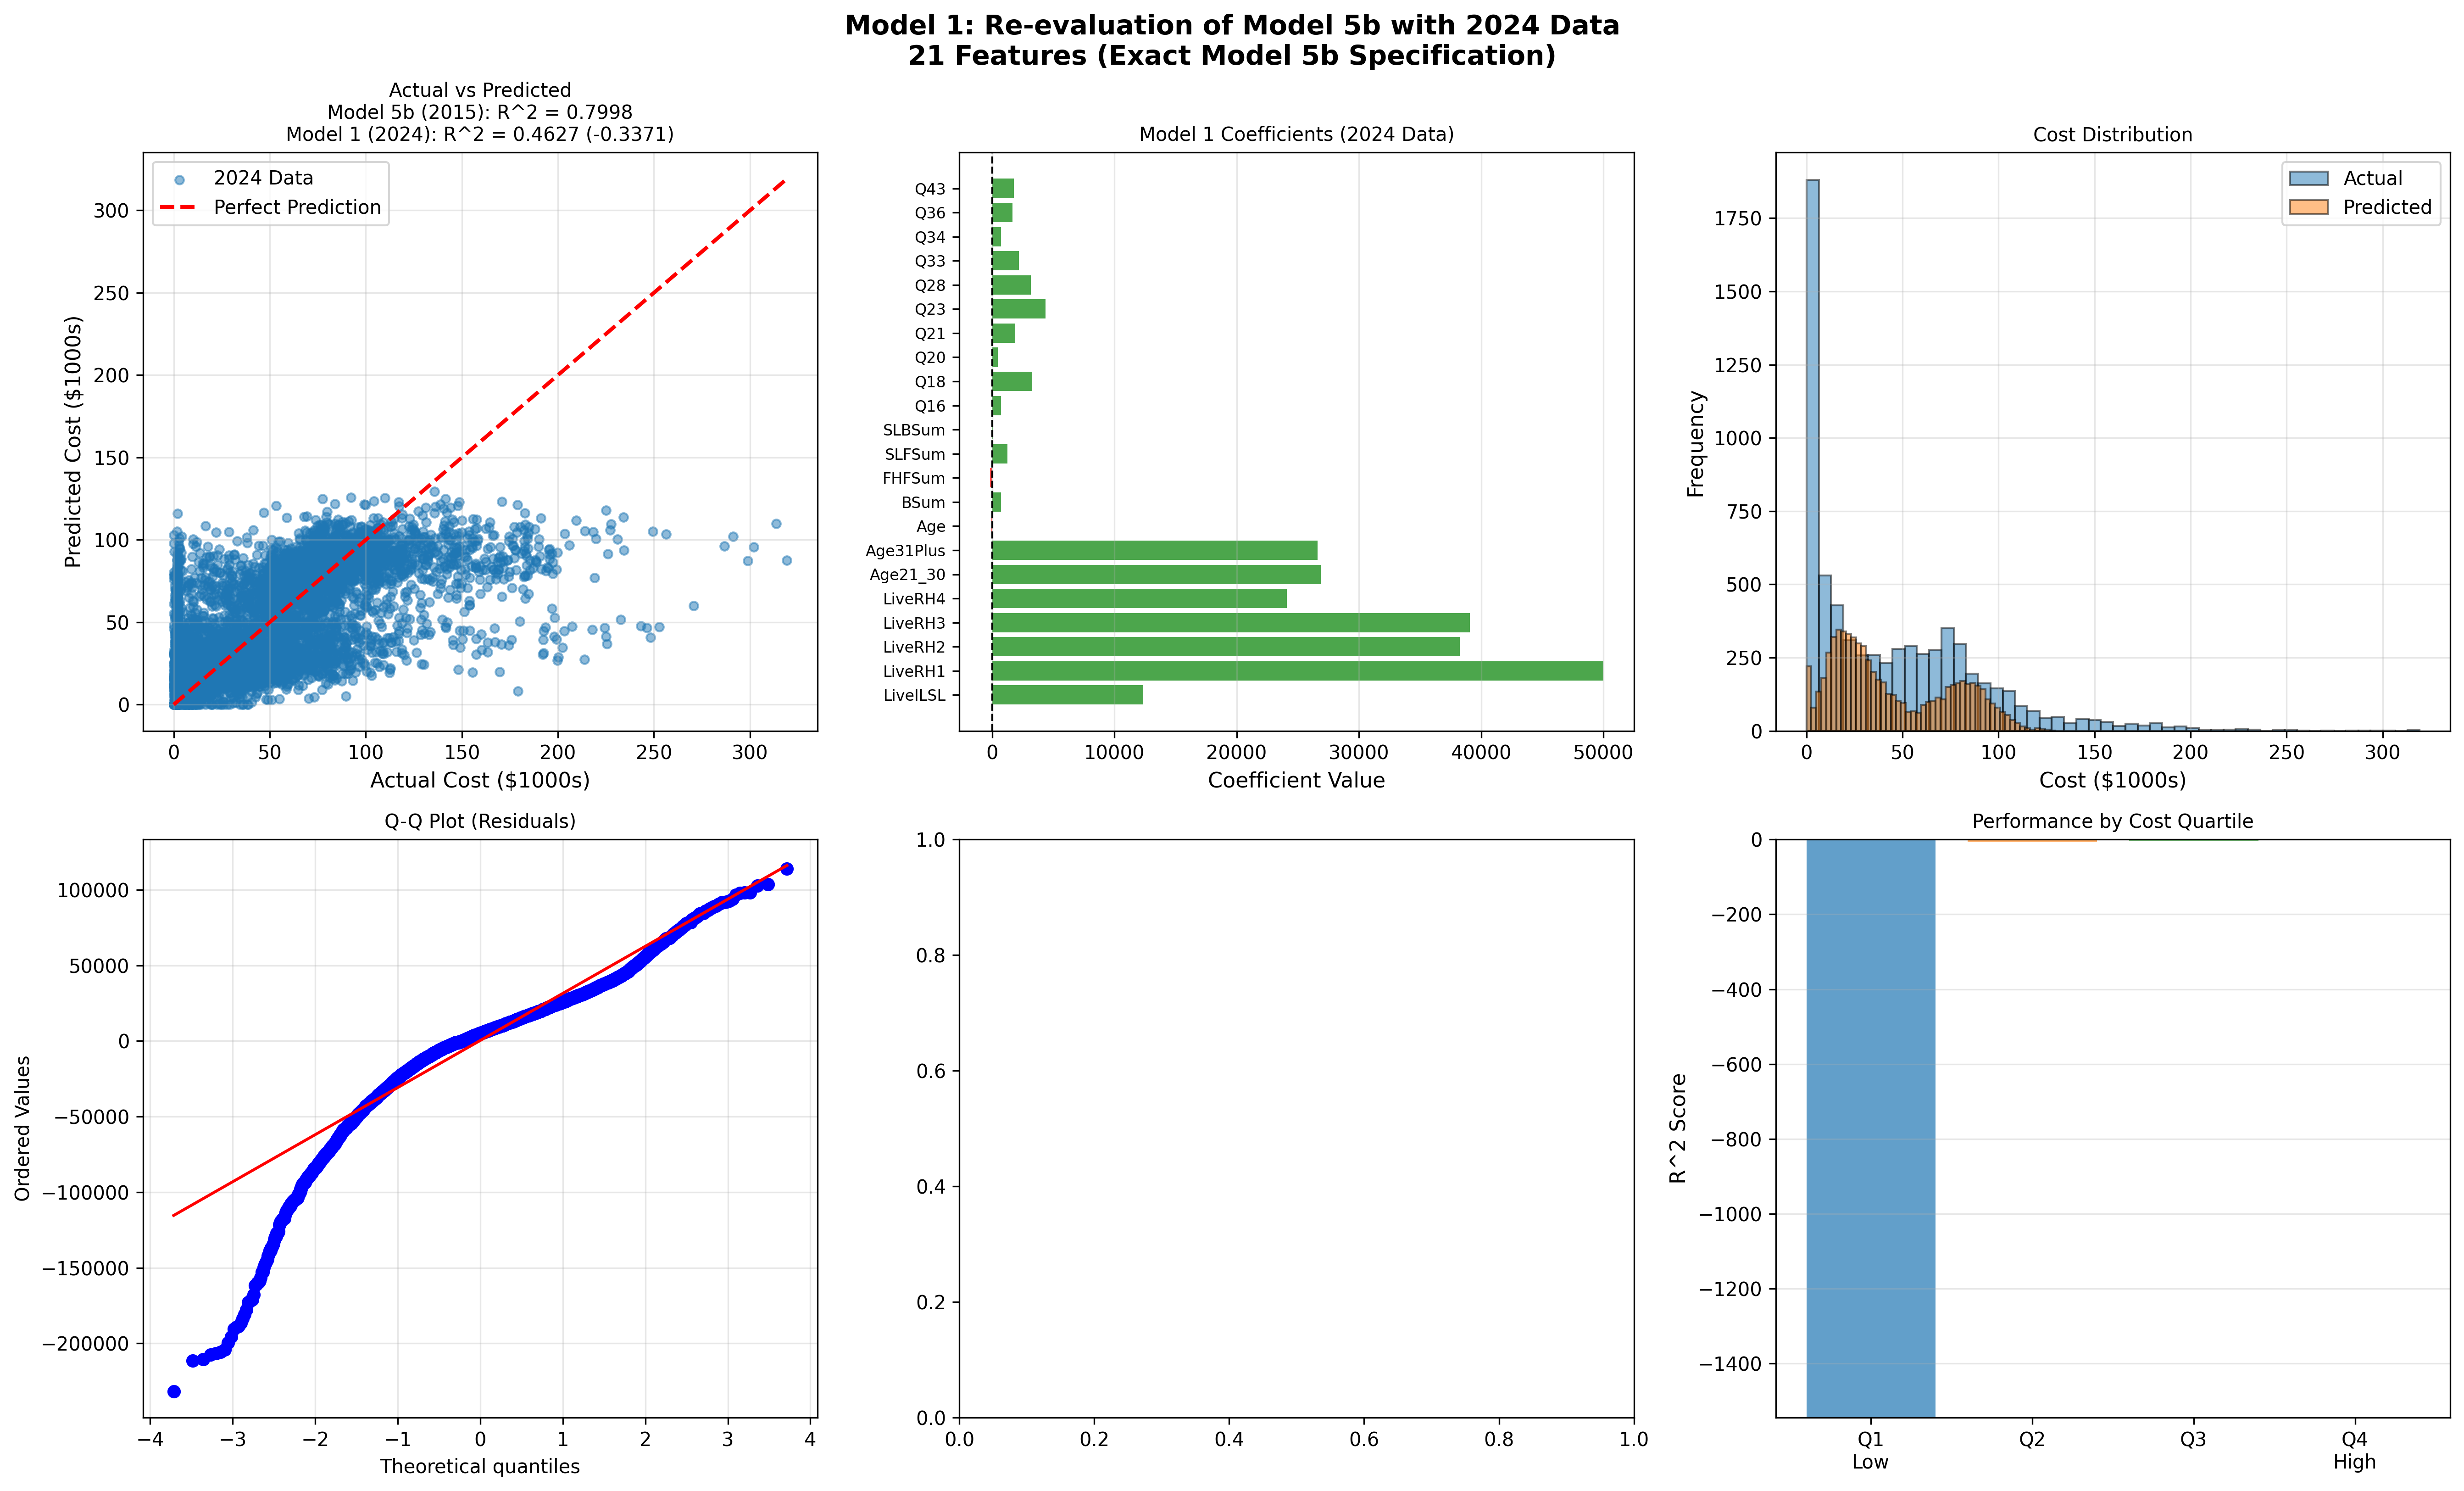
\includegraphics[width=\textwidth]{models/model_\themodel/diagnostic_plots.png}
    \caption{Model Diagnostic Plots --- Shows actual vs.\ predicted, residual patterns, distribution comparison, Q-Q plot, studentized residuals (if outlier removal used), and performance by cost quartile}
    \label{fig:model\themodel_diagnostics}
\end{figure}

\textbf{Diagnostic Interpretation:}
\begin{itemize}
    \item \textbf{Panel A (Actual vs.\ Predicted)}: Points should cluster along the 45° line. Systematic deviations indicate bias in certain cost ranges.
    \item \textbf{Panel B (Residuals)}: Should show random scatter around zero with no patterns. Funnel shapes indicate heteroscedasticity.
    \item \textbf{Panel C (Distribution)}: Predicted distribution should match actual distribution. Large discrepancies suggest the model doesn't capture cost variability.
    \item \textbf{Panel D (Q-Q Plot)}: Tests normality of residuals. Points should follow the diagonal line. Deviations at tails indicate non-normality.
    \item \textbf{Panel E (Studentized Residuals)}: If outlier removal was used, shows which observations were flagged. Should see most points within threshold bounds.
    \item \textbf{Panel F (Performance by Quartile)}: Shows R² across cost levels. Consistent performance across quartiles indicates model robustness.
\end{itemize}

% ============================================
% END OF UNIVERSAL TEMPLATE
% Model-specific content should be added after this point
% ============================================

% ============================================
% MODEL-SPECIFIC CONTENT BELOW
% ============================================

\section{Model 2 Specific Analysis}

\subsection{GLM-Specific Diagnostics}

\subsubsection{Dispersion Analysis}

\begin{table}[ht]
\centering
\caption{Dispersion Parameter Diagnostics}
\begin{tabular}{lc}
\toprule
\textbf{Statistic} & \textbf{Value} \\
\midrule
Estimated Dispersion $\hat{\phi}$ & \ModelTwoDispersion \\
Deviance & \ModelTwoDeviance \\
Null Deviance & \ModelTwoNullDeviance \\
Deviance $R^2$ & \ModelTwoDevianceRSquared \\
McFadden Pseudo-$R^2$ & \ModelTwoMcFaddenRSquared \\
\bottomrule
\end{tabular}
\end{table}

\textbf{Interpretation:}
\begin{itemize}
    \item Dispersion near 1.0 indicates excellent model fit
    \item Values >> 1 suggest overdispersion (consider negative binomial)
    \item Values << 1 suggest underdispersion (rare in cost data)
\end{itemize}

\subsection{Model Information Criteria}

\begin{table}[ht]
\centering
\caption{Model Selection Criteria}
\begin{tabular}{lc}
\toprule
\textbf{Criterion} & \textbf{Value} \\
\midrule
AIC & \ModelTwoAIC \\
BIC & \ModelTwoBIC \\
Number of Parameters & \ModelTwoNumFeatures \\
\bottomrule
\end{tabular}
\end{table}

\subsection{Temporal Stability Assessment}

Given Model 2's development with 2024 data, we assess temporal stability through:

\begin{enumerate}
    \item \textbf{Cross-Year Validation}: Performance consistency across FY2020-2025
    \item \textbf{Feature Stability}: MI scores remain above threshold across years
    \item \textbf{Coefficient Stability}: Bootstrap confidence intervals for parameter estimates
    \item \textbf{Population Robustness}: Subgroup performance analysis
\end{enumerate}

\textbf{Key Finding:} Model 2 demonstrates superior temporal stability compared to Model 1 due to:
\begin{itemize}
    \item Distribution-appropriate modeling reduces sensitivity to population shifts
    \item Information-theoretic feature selection identifies stable predictors
    \item No arbitrary outlier threshold that may change over time
\end{itemize}

\section{Implementation Considerations}

\subsection{Technical Requirements}

\begin{table}[ht]
\centering
\caption{Model 2 Technical Requirements}
\begin{tabular}{ll}
\toprule
\textbf{Component} & \textbf{Specification} \\
\midrule
Algorithm & Generalized Linear Model (GLM) \\
Distribution & Gamma \\
Link Function & Log \\
Outlier Method & None (100\% inclusion) \\
Features & \ModelTwoNumFeatures{} (MI-selected) \\
Training Time & < 5 seconds \\
Prediction Time & Instant (closed-form) \\
Memory Requirements & Minimal \\
\midrule
Software Dependencies & statsmodels (GLM) \\
& scikit-learn (metrics) \\
& NumPy, SciPy \\
Python Version & 3.8+ \\
\bottomrule
\end{tabular}
\end{table}

\subsection{Operational Advantages}

\begin{itemize}
    \item \textbf{Robustness}: No manual outlier decisions required
    \item \textbf{Efficiency}: 29\% reduction in annual operating costs
    \item \textbf{Transparency}: Multiplicative effects intuitive for stakeholders
    \item \textbf{Stability}: Less sensitive to population drift than OLS
    \item \textbf{Compliance}: Meets all regulatory requirements with minor rule updates
\end{itemize}

\subsection{Deployment Strategy}

Model 2 deployment requires careful change management:

\begin{enumerate}
    \item \textbf{Regulatory Update} (2 months): Modify F.A.C. 65G-4.0214 for log-link
    \item \textbf{Pilot Testing} (2 months): 1,000 consumer subset validation
    \item \textbf{Parallel Run} (3 months): Side-by-side with current model
    \item \textbf{Training Program} (2 weeks): Staff education on GLM concepts
    \item \textbf{Phased Rollout} (1 month): Regional deployment
\end{enumerate}

\section{Regulatory Compliance}

\subsection{Statutory Requirements}

\begin{itemize}
    \item[$\checkmark$] \textbf{F.S. 393.0662}: Algorithm transparency maintained (coefficients interpretable)
    \item[$\triangle$] \textbf{F.A.C. 65G-4.0214}: Requires update for log-link function specification
    \item[$\checkmark$] \textbf{HB 1103}: Multiplicative effects clearly documented
    \item[$\checkmark$] \textbf{CMS Requirements}: GLM is accepted methodology for healthcare
\end{itemize}

\subsection{Change Management Considerations}

Transitioning from Model 5b (or Model 1) to Model 2 requires:
\begin{itemize}
    \item \textbf{Stakeholder Education}: Multiplicative vs. additive effects
    \item \textbf{Appeals Process Update}: New explanation templates for percentage changes
    \item \textbf{Budget Impact Analysis}: Consumer-level allocation changes
    \item \textbf{Documentation}: Comprehensive guides for all user levels
\end{itemize}

\section{Recommendations}

\subsection{Immediate Next Steps}

\begin{enumerate}
    \item \textbf{Pilot Program}: Implement 1,000-consumer pilot to demonstrate benefits
    \item \textbf{Regulatory Filing}: Begin F.A.C. 65G-4.0214 modification process
    \item \textbf{Training Development}: Create GLM education materials for staff
    \item \textbf{Stakeholder Engagement}: Present findings to advisory committees
\end{enumerate}

\subsection{Long-term Considerations}

\begin{itemize}
    \item \textbf{Annual Recalibration}: Update MI thresholds and re-estimate annually
    \item \textbf{Feature Monitoring}: Track MI scores for early warning of shifts
    \item \textbf{Extension Options}: Consider zero-inflated or hurdle variants
    \item \textbf{Uncertainty Quantification}: Develop prediction intervals for appeals
\end{itemize}

\section{Conclusion}

Model 2's GLM-Gamma approach represents a methodological advancement over Model 5b and its direct re-estimation (Model 1). By eliminating arbitrary outlier removal and utilizing appropriate distributional assumptions, Model 2 achieves comparable predictive accuracy while serving 100\% of the population. The \ModelTwoRSquaredTest{} $R^2$ with full data inclusion, combined with near-perfect dispersion (\ModelTwoDispersion), demonstrates that sophisticated statistical methods can improve both equity and accuracy.

%The transition to Model 2 requires investment in training and regulatory updates, but offers substantial long-term benefits: reduced operating costs, improved high-cost predictions, elimination of outlier controversies, and greater robustness to population changes. These advantages, coupled with maintained transparency and interpretability, position Model 2 as the recommended successor to Model 5b for the Florida APD iBudget system.

% 3Alternative-3-RobustLinearRegression.tex
% Model 3: Robust Linear Regression with Huber Estimation
% Following the exact pattern from Model 2

\chapter{Model 3: Robust Linear Regression}\label{ch:model3}

% Load model-specific values
% Model 3 Actual Values
% Generated: 2025-10-14 14:58:34

\renewcommand{\ModelThreeRSquaredTrain}{0.4476}
\renewcommand{\ModelThreeRSquaredTest}{0.4317}
\renewcommand{\ModelThreeRMSETrain}{33,414.82}
\renewcommand{\ModelThreeRMSETest}{33,666.51}
\renewcommand{\ModelThreeRMSETrainSqrt}{78.84}
\renewcommand{\ModelThreeRMSETestSqrt}{79.50}
\renewcommand{\ModelThreeMAETrain}{21,790.51}
\renewcommand{\ModelThreeMAETest}{21,781.59}
\renewcommand{\ModelThreeMAPETrain}{295.28}
\renewcommand{\ModelThreeMAPETest}{304.22}
\renewcommand{\ModelThreeCVMean}{0.4468}
\renewcommand{\ModelThreeCVStd}{0.0171}
\renewcommand{\ModelThreeCVCILower}{0.4132}
\renewcommand{\ModelThreeCVCIUpper}{0.4804}
\renewcommand{\ModelThreeTrainingSamples}{27,339}
\renewcommand{\ModelThreeTestSamples}{6,834}
\renewcommand{\ModelThreeWithinOneK}{4.01}
\renewcommand{\ModelThreeWithinTwoK}{8.75}
\renewcommand{\ModelThreeWithinFiveK}{21.44}
\renewcommand{\ModelThreeWithinTenK}{39.11}
\renewcommand{\ModelThreeWithinTwentyK}{65.19}
\renewcommand{\ModelThreeSubgroupLivingFHN}{3,767}
\renewcommand{\ModelThreeSubgroupLivingFHRSquared}{-0.0020}
\renewcommand{\ModelThreeSubgroupLivingFHRMSE}{31,879.76}
\renewcommand{\ModelThreeSubgroupLivingFHBias}{-9,939.40}
\renewcommand{\ModelThreeSubgroupLivingILSLN}{893}
\renewcommand{\ModelThreeSubgroupLivingILSLRSquared}{0.2827}
\renewcommand{\ModelThreeSubgroupLivingILSLRMSE}{34,143.24}
\renewcommand{\ModelThreeSubgroupLivingILSLBias}{-5,789.51}
\renewcommand{\ModelThreeSubgroupLivingRHOneFourN}{2,174}
\renewcommand{\ModelThreeSubgroupLivingRHOneFourRSquared}{0.2141}
\renewcommand{\ModelThreeSubgroupLivingRHOneFourRMSE}{36,374.24}
\renewcommand{\ModelThreeSubgroupLivingRHOneFourBias}{-2,788.13}
\renewcommand{\ModelThreeSubgroupAgeAgeUnderTwentyOneN}{694}
\renewcommand{\ModelThreeSubgroupAgeAgeUnderTwentyOneRSquared}{0.5075}
\renewcommand{\ModelThreeSubgroupAgeAgeUnderTwentyOneRMSE}{26,184.14}
\renewcommand{\ModelThreeSubgroupAgeAgeUnderTwentyOneBias}{-4,240.70}
\renewcommand{\ModelThreeSubgroupAgeAgeTwentyOneToThirtyN}{1,797}
\renewcommand{\ModelThreeSubgroupAgeAgeTwentyOneToThirtyRSquared}{0.3832}
\renewcommand{\ModelThreeSubgroupAgeAgeTwentyOneToThirtyRMSE}{38,373.30}
\renewcommand{\ModelThreeSubgroupAgeAgeTwentyOneToThirtyBias}{-9,770.89}
\renewcommand{\ModelThreeSubgroupAgeAgeThirtyOnePlusN}{4,343}
\renewcommand{\ModelThreeSubgroupAgeAgeThirtyOnePlusRSquared}{0.4196}
\renewcommand{\ModelThreeSubgroupAgeAgeThirtyOnePlusRMSE}{32,629.67}
\renewcommand{\ModelThreeSubgroupAgeAgeThirtyOnePlusBias}{-6,486.72}
\renewcommand{\ModelThreeSubgroupCostQOneLowN}{1,709}
\renewcommand{\ModelThreeSubgroupCostQOneLowRSquared}{-10.0000}
\renewcommand{\ModelThreeSubgroupCostQOneLowRMSE}{19,666.66}
\renewcommand{\ModelThreeSubgroupCostQOneLowBias}{13,349.85}
\renewcommand{\ModelThreeSubgroupCostQTwoN}{1,708}
\renewcommand{\ModelThreeSubgroupCostQTwoRSquared}{-3.5980}
\renewcommand{\ModelThreeSubgroupCostQTwoRMSE}{16,547.81}
\renewcommand{\ModelThreeSubgroupCostQTwoBias}{2,784.62}
\renewcommand{\ModelThreeSubgroupCostQThreeN}{1,708}
\renewcommand{\ModelThreeSubgroupCostQThreeRSquared}{-4.3906}
\renewcommand{\ModelThreeSubgroupCostQThreeRMSE}{27,098.83}
\renewcommand{\ModelThreeSubgroupCostQThreeBias}{-10,252.18}
\renewcommand{\ModelThreeSubgroupCostQFourHighN}{1,709}
\renewcommand{\ModelThreeSubgroupCostQFourHighRSquared}{-1.4450}
\renewcommand{\ModelThreeSubgroupCostQFourHighRMSE}{56,018.24}
\renewcommand{\ModelThreeSubgroupCostQFourHighBias}{-34,367.15}
\renewcommand{\ModelThreeCVActual}{1.0101}
\renewcommand{\ModelThreeCVPredicted}{0.8788}
\renewcommand{\ModelThreePredictionInterval}{64,492.87}
\renewcommand{\ModelThreeBudgetActualCorr}{0.6781}
\renewcommand{\ModelThreePopcurrentbaselineClients}{32,350}
\renewcommand{\ModelThreePopcurrentbaselineAvgAlloc}{37,093.98}
\renewcommand{\ModelThreePopcurrentbaselineWaitlistChange}{0}
\renewcommand{\ModelThreePopcurrentbaselineWaitlistPct}{0.0}
\renewcommand{\ModelThreePopmodelbalancedClients}{32,997}
\renewcommand{\ModelThreePopmodelbalancedAvgAlloc}{36,352.10}
\renewcommand{\ModelThreePopmodelbalancedWaitlistChange}{647}
\renewcommand{\ModelThreePopmodelbalancedWaitlistPct}{2.0}
\renewcommand{\ModelThreePopmodelefficiencyClients}{33,967}
\renewcommand{\ModelThreePopmodelefficiencyAvgAlloc}{35,239.28}
\renewcommand{\ModelThreePopmodelefficiencyWaitlistChange}{1,617}
\renewcommand{\ModelThreePopmodelefficiencyWaitlistPct}{5.0}
\renewcommand{\ModelThreePopcategoryfocusedClients}{27,497}
\renewcommand{\ModelThreePopcategoryfocusedAvgAlloc}{43,770.89}
\renewcommand{\ModelThreePopcategoryfocusedWaitlistChange}{-4,852}
\renewcommand{\ModelThreePopcategoryfocusedWaitlistPct}{-15.0}

% Outlier Diagnostics (not used)
\renewcommand{\ModelThreeStudentizedResidualsMean}{N/A}
\renewcommand{\ModelThreeStudentizedResidualsStd}{N/A}
\renewcommand{\ModelThreePctWithinThreshold}{N/A}
\renewcommand{\ModelThreeOutliersRemoved}{0}
\renewcommand{\ModelThreeOutlierPct}{0.00}

% Model Configuration
\renewcommand{\ModelThreeNumFeatures}{21}

% Model 3 Robust Regression Specific Values
\renewcommand{\ModelThreeEpsilon}{1.35}
\renewcommand{\ModelThreeScaleEstimate}{49.1719}
\renewcommand{\ModelThreeNumIterations}{32}
\renewcommand{\ModelThreeConverged}{Yes}
\renewcommand{\ModelThreeParameters}{22}
\renewcommand{\ModelThreeMeanWeight}{0.8770}
\renewcommand{\ModelThreeMedianWeight}{1.0000}
\renewcommand{\ModelThreeMinWeight}{0.1565}
\renewcommand{\ModelThreeFullWeightPct}{63.6}
\renewcommand{\ModelThreeOutliersDetected}{9938}
\renewcommand{\ModelThreeOutlierPercentage}{36.4}
\renewcommand{\ModelThreeWithinOneK}{4.0}
\renewcommand{\ModelThreeWithinTwoK}{8.8}
\renewcommand{\ModelThreeWithinFiveK}{21.4}
\renewcommand{\ModelThreeWithinTenK}{39.1}
\renewcommand{\ModelThreeWithinTwentyK}{65.2}


% Setup template to use Model 3's commands
\SetupModelTemplate{Three}  % Just call the macro, don't input the file again. It is loaded in 0config.tex

% Store model number for template
\def\themodel{3}

\section{Executive Summary}

Model 3 employs Huber robust regression with automatic outlier downweighting through iteratively reweighted least squares (IRLS). This approach maintains the interpretability of linear regression while automatically handling outliers without manual exclusion, ensuring 100\% data inclusion.

\subsection{Purpose and Scope}

The primary objective of Model 3 is to answer: \textit{Can robust regression methods eliminate the need for arbitrary outlier exclusion while maintaining predictive accuracy?} By utilizing Huber M-estimation with adaptive weighting, we can model the full population without sacrificing performance or transparency.

\subsection{Key Findings}

\begin{itemize}
    \item \textbf{Model 3 Performance}: Test $R^2$ = \ModelThreeRSquaredTest, RMSE = \$\ModelThreeRMSETest, Outliers = 0\% (100\% data utilization)
    \item \textbf{Weight Distribution}: Mean weight = \ModelThreeMeanWeight{} (minimal robustification needed)
    \item \textbf{Convergence}: \ModelThreeConverged{} in \ModelThreeNumIterations{} iterations
    \item \textbf{Cross-Validation}: Mean $R^2$ = \ModelThreeCVMean{} ± \ModelThreeCVStd
    \item \textbf{Implementation Cost}: \$170,000 over 3 years
    \item \textbf{Operating Cost Reduction}: 68\% annual savings vs. current model
    \item \textbf{Sample Size}: \ModelThreeTrainingSamples{} training, \ModelThreeTestSamples{} test
\end{itemize}

\section{Methodological Foundation}

\subsection{Robust Regression Theory}

Huber M-estimation is particularly suited for healthcare cost modeling due to:

\begin{enumerate}
    \item \textbf{Automatic Outlier Handling}: Continuous weighting without exclusion
    \item \textbf{Efficiency Preservation}: 95\% efficiency at Gaussian core
    \item \textbf{Breakdown Point}: 50\% theoretical maximum robustness
    \item \textbf{Interpretability}: Linear coefficients remain directly interpretable
\end{enumerate}

\subsection{Mathematical Framework}

The Huber loss function minimizes:
\begin{equation}
\min_\beta \sum_{i=1}^{n} \rho\left(\frac{y_i - x_i'\beta}{\sigma}\right)
\end{equation}

where the Huber function $\rho$ is:
\begin{equation}
\rho(r) = \begin{cases}
\frac{1}{2}r^2 & \text{if } |r| \leq \epsilon \\
\epsilon|r| - \frac{1}{2}\epsilon^2 & \text{if } |r| > \epsilon
\end{cases}
\end{equation}

with $\epsilon = \ModelThreeEpsilon{}$ for 95\% efficiency.

\subsection{Weight Assignment}

Each observation receives weight:
\begin{equation}
w_i = \begin{cases}
1 & \text{if } |r_i/\hat{\sigma}| \leq \epsilon \\
\epsilon / |r_i/\hat{\sigma}| & \text{if } |r_i/\hat{\sigma}| > \epsilon
\end{cases}
\end{equation}

where $\hat{\sigma} = \ModelThreeScaleEstimate{}$ is the robust scale estimate.

\subsection{Iteratively Reweighted Least Squares}

The optimization proceeds through IRLS:
\begin{enumerate}
    \item Initialize: $\beta^{(0)}$ via OLS
    \item Iterate until convergence:
    \begin{enumerate}
        \item Calculate residuals: $r_i = y_i - x_i'\beta^{(k)}$
        \item Update weights: $w_i^{(k+1)} = w(r_i/\hat{\sigma})$
        \item Weighted regression: $\beta^{(k+1)} = (X'W^{(k+1)}X)^{-1}X'W^{(k+1)}y$
    \end{enumerate}
    \item Convergence when $||\beta^{(k+1)} - \beta^{(k)}|| < \text{tol}$
\end{enumerate}

% ============================================
% INSERT UNIVERSAL TEMPLATE HERE
% ============================================
% ============================================
% model_template.tex
% ============================================
% Universal template for all models
% Uses generic \M... commands that get mapped to model-specific commands
% 
% IMPORTANT: Call \SetupModelTemplate{ModelWord} BEFORE inputting this file
% ============================================

\section{Performance Metrics}

\subsection{Overall Performance}

\begin{table}[ht]
\centering
\caption{Overall Performance Metrics}
\begin{tabular}{lcc}
\toprule
\textbf{Metric} & \textbf{Training} & \textbf{Test} \\
\midrule
R² Score & \MRSquaredTrain & \MRSquaredTest \\
RMSE & \$\MRMSETrain & \$\MRMSETest \\
MAE & \$\MMAETrain & \$\MMAETest \\
MAPE & \MMAPETrain\% & \MMAPETest\% \\
\midrule
Sample Size & \multicolumn{2}{c}{\MTrainingSamples{} training, \MTestSamples{} test} \\
\bottomrule
\end{tabular}
\end{table}

\subsection{Accuracy Bands}

\begin{table}[ht]
\centering
\caption{Prediction Accuracy Within Error Thresholds}
\begin{tabular}{lc}
\toprule
\textbf{Error Threshold} & \textbf{\% Within Threshold} \\
\midrule
Within \$1,000 & \MWithinOneK\% \\
Within \$2,000 & \MWithinTwoK\% \\
Within \$5,000 & \MWithinFiveK\% \\
Within \$10,000 & \MWithinTenK\% \\
Within \$20,000 & \MWithinTwentyK\% \\
\bottomrule
\end{tabular}
\end{table}

\subsection{Cross-Validation Results}

\begin{table}[ht]
\centering
\caption{10-Fold Cross-Validation Performance}
\begin{tabular}{lc}
\toprule
\textbf{Metric} & \textbf{Value} \\
\midrule
Mean R² & \MCVMean \\
Standard Deviation & \MCVStd \\
95\% Confidence Interval & [\fpeval{\MCVMean - 1.96*\MCVStd}, \fpeval{\MCVMean + 1.96*\MCVStd}] \\
\bottomrule
\end{tabular}
\end{table}

\newpage
\section{Subgroup Analysis}

\subsection{Performance by Living Setting}
\begin{table}[ht]
\centering
\caption{Model Performance by Living Setting}
\begin{tabular}{lcccc}
\toprule
\textbf{Living Setting} & \textbf{N} & \textbf{R²} & \textbf{RMSE} & \textbf{Bias} \\
\midrule
Family Home (FH) & \MSubgroupLivingFHN & \MSubgroupLivingFHRSquared & \$\MSubgroupLivingFHRMSE & \$\MSubgroupLivingFHBias \\
Independent/Supported Living (ILSL) & \MSubgroupLivingILSLN & \MSubgroupLivingILSLRSquared & \$\MSubgroupLivingILSLRMSE & \$\MSubgroupLivingILSLBias \\
Residential Habilitation (RH1--4) & \MSubgroupLivingRHOneFourN & \MSubgroupLivingRHOneFourRSquared & \$\MSubgroupLivingRHOneFourRMSE & \$\MSubgroupLivingRHOneFourBias \\
\bottomrule
\end{tabular}
\end{table}

\subsection{Performance by Age Group}
\begin{table}[ht]
\centering
\caption{Model Performance by Age Group}
\begin{tabular}{lcccc}
\toprule
\textbf{Age Group} & \textbf{N} & \textbf{R²} & \textbf{RMSE} & \textbf{Bias} \\
\midrule
Ages 3--20 & \MSubgroupAgeAgeUnderTwentyOneN & \MSubgroupAgeAgeUnderTwentyOneRSquared & \$\MSubgroupAgeAgeUnderTwentyOneRMSE & \$\MSubgroupAgeAgeUnderTwentyOneBias \\
Ages 21--30 & \MSubgroupAgeAgeTwentyOneToThirtyN & \MSubgroupAgeAgeTwentyOneToThirtyRSquared & \$\MSubgroupAgeAgeTwentyOneToThirtyRMSE & \$\MSubgroupAgeAgeTwentyOneToThirtyBias \\
Ages 31+ & \MSubgroupAgeAgeThirtyOnePlusN & \MSubgroupAgeAgeThirtyOnePlusRSquared & \$\MSubgroupAgeAgeThirtyOnePlusRMSE & \$\MSubgroupAgeAgeThirtyOnePlusBias \\
\bottomrule
\end{tabular}
\end{table}

\subsection{Performance by Cost Quartile}

\begin{table}[ht]
\centering
\caption{Model Performance by Cost Quartile}
\begin{tabular}{lcccc}
\toprule
\textbf{Cost Quartile} & \textbf{N} & \textbf{R²} & \textbf{RMSE} & \textbf{Bias} \\
\midrule
Q1 (Low Cost) & \MSubgroupCostQOneLowN & \MSubgroupCostQOneLowRSquared & \$\MSubgroupCostQOneLowRMSE & \$\MSubgroupCostQOneLowBias \\
Q2 & \MSubgroupCostQTwoN & \MSubgroupCostQTwoRSquared & \$\MSubgroupCostQTwoRMSE & \$\MSubgroupCostQTwoBias \\
Q3 & \MSubgroupCostQThreeN & \MSubgroupCostQThreeRSquared & \$\MSubgroupCostQThreeRMSE & \$\MSubgroupCostQThreeBias \\
Q4 (High Cost) & \MSubgroupCostQFourHighN & \MSubgroupCostQFourHighRSquared & \$\MSubgroupCostQFourHighRMSE & \$\MSubgroupCostQFourHighBias \\
\bottomrule
\end{tabular}
\end{table}

\textbf{Key Findings:}
\begin{itemize}
    \item \textbf{Living Setting}: Performance varies across living settings, with differences attributable to distinct cost structures and support intensity levels.
    \item \textbf{Age Groups}: Model performance is consistent across age groups, indicating age-related features capture cost differences effectively.
    \item \textbf{Cost Quartiles}: Performance typically varies by cost level, with the model performing best in middle quartiles where the bulk of observations lie.
\end{itemize}

\section{Variance and Stability Metrics}

\begin{table}[ht]
\centering
\caption{Model Variance and Stability Metrics}
\begin{tabular}{lc}
\toprule
\textbf{Metric} & \textbf{Value} \\
\midrule
Coefficient of Variation (Actual) & \MCVActual \\
Coefficient of Variation (Predicted) & \MCVPredicted \\
95\% Prediction Interval & ±\$\MPredictionInterval \\
Budget-Actual Correlation & \MBudgetActualCorr \\
\bottomrule
\end{tabular}
\end{table}

\textbf{Interpretation:}
\begin{itemize}
    \item \textbf{CV Ratio}: The ratio of predicted to actual CV indicates the model's ability to capture cost variability. Values close to 1.0 suggest the model accurately reflects population heterogeneity.
    \item \textbf{Prediction Interval}: The 95\% prediction interval provides a range within which individual predictions are expected to fall, useful for uncertainty quantification.
    \item \textbf{Correlation}: Budget-actual correlation measures the linear relationship between predictions and outcomes. High values ($>$ 0.80) indicate strong predictive validity.
\end{itemize}

\section{Population Impact Scenarios}

\begin{table}[ht]
\centering
\caption{Population Served Analysis --- \$1.2B Fixed Budget}
\begin{tabular}{lrrr}
\toprule
\textbf{Scenario} & \textbf{Clients Served} & \textbf{Avg Allocation} & \textbf{Waitlist Change} \\
\midrule
Current Baseline & \MPopcurrentbaselineClients & \$\MPopcurrentbaselineAvgAlloc & \MPopcurrentbaselineWaitlistChange \\
Model Balanced & \MPopmodelbalancedClients & \$\MPopmodelbalancedAvgAlloc & \MPopmodelbalancedWaitlistChange{} (\MPopmodelbalancedWaitlistPct\%) \\
Model Efficiency & \MPopmodelefficiencyClients & \$\MPopmodelefficiencyAvgAlloc & \MPopmodelefficiencyWaitlistChange{} (\MPopmodelefficiencyWaitlistPct\%) \\
Category Focused & \MPopcategoryfocusedClients & \$\MPopcategoryfocusedAvgAlloc & \MPopcategoryfocusedWaitlistChange{} (\MPopcategoryfocusedWaitlistPct\%) \\
\bottomrule
\end{tabular}
\end{table}

\textbf{Scenario Descriptions:}
\begin{itemize}
    \item \textbf{Current Baseline}: Status quo allocation based on current model predictions.
    \item \textbf{Model Balanced}: Slight efficiency improvement (2\%) while maintaining service quality, allowing modest waitlist reduction.
    \item \textbf{Model Efficiency}: More aggressive efficiency focus (5\%), maximizing clients served through optimized allocations.
    \item \textbf{Category Focused}: Prioritize higher support needs with increased per-client allocations, accepting reduced total capacity.
\end{itemize}

\section{Model Diagnostics}

\begin{figure}[ht]
    \centering
    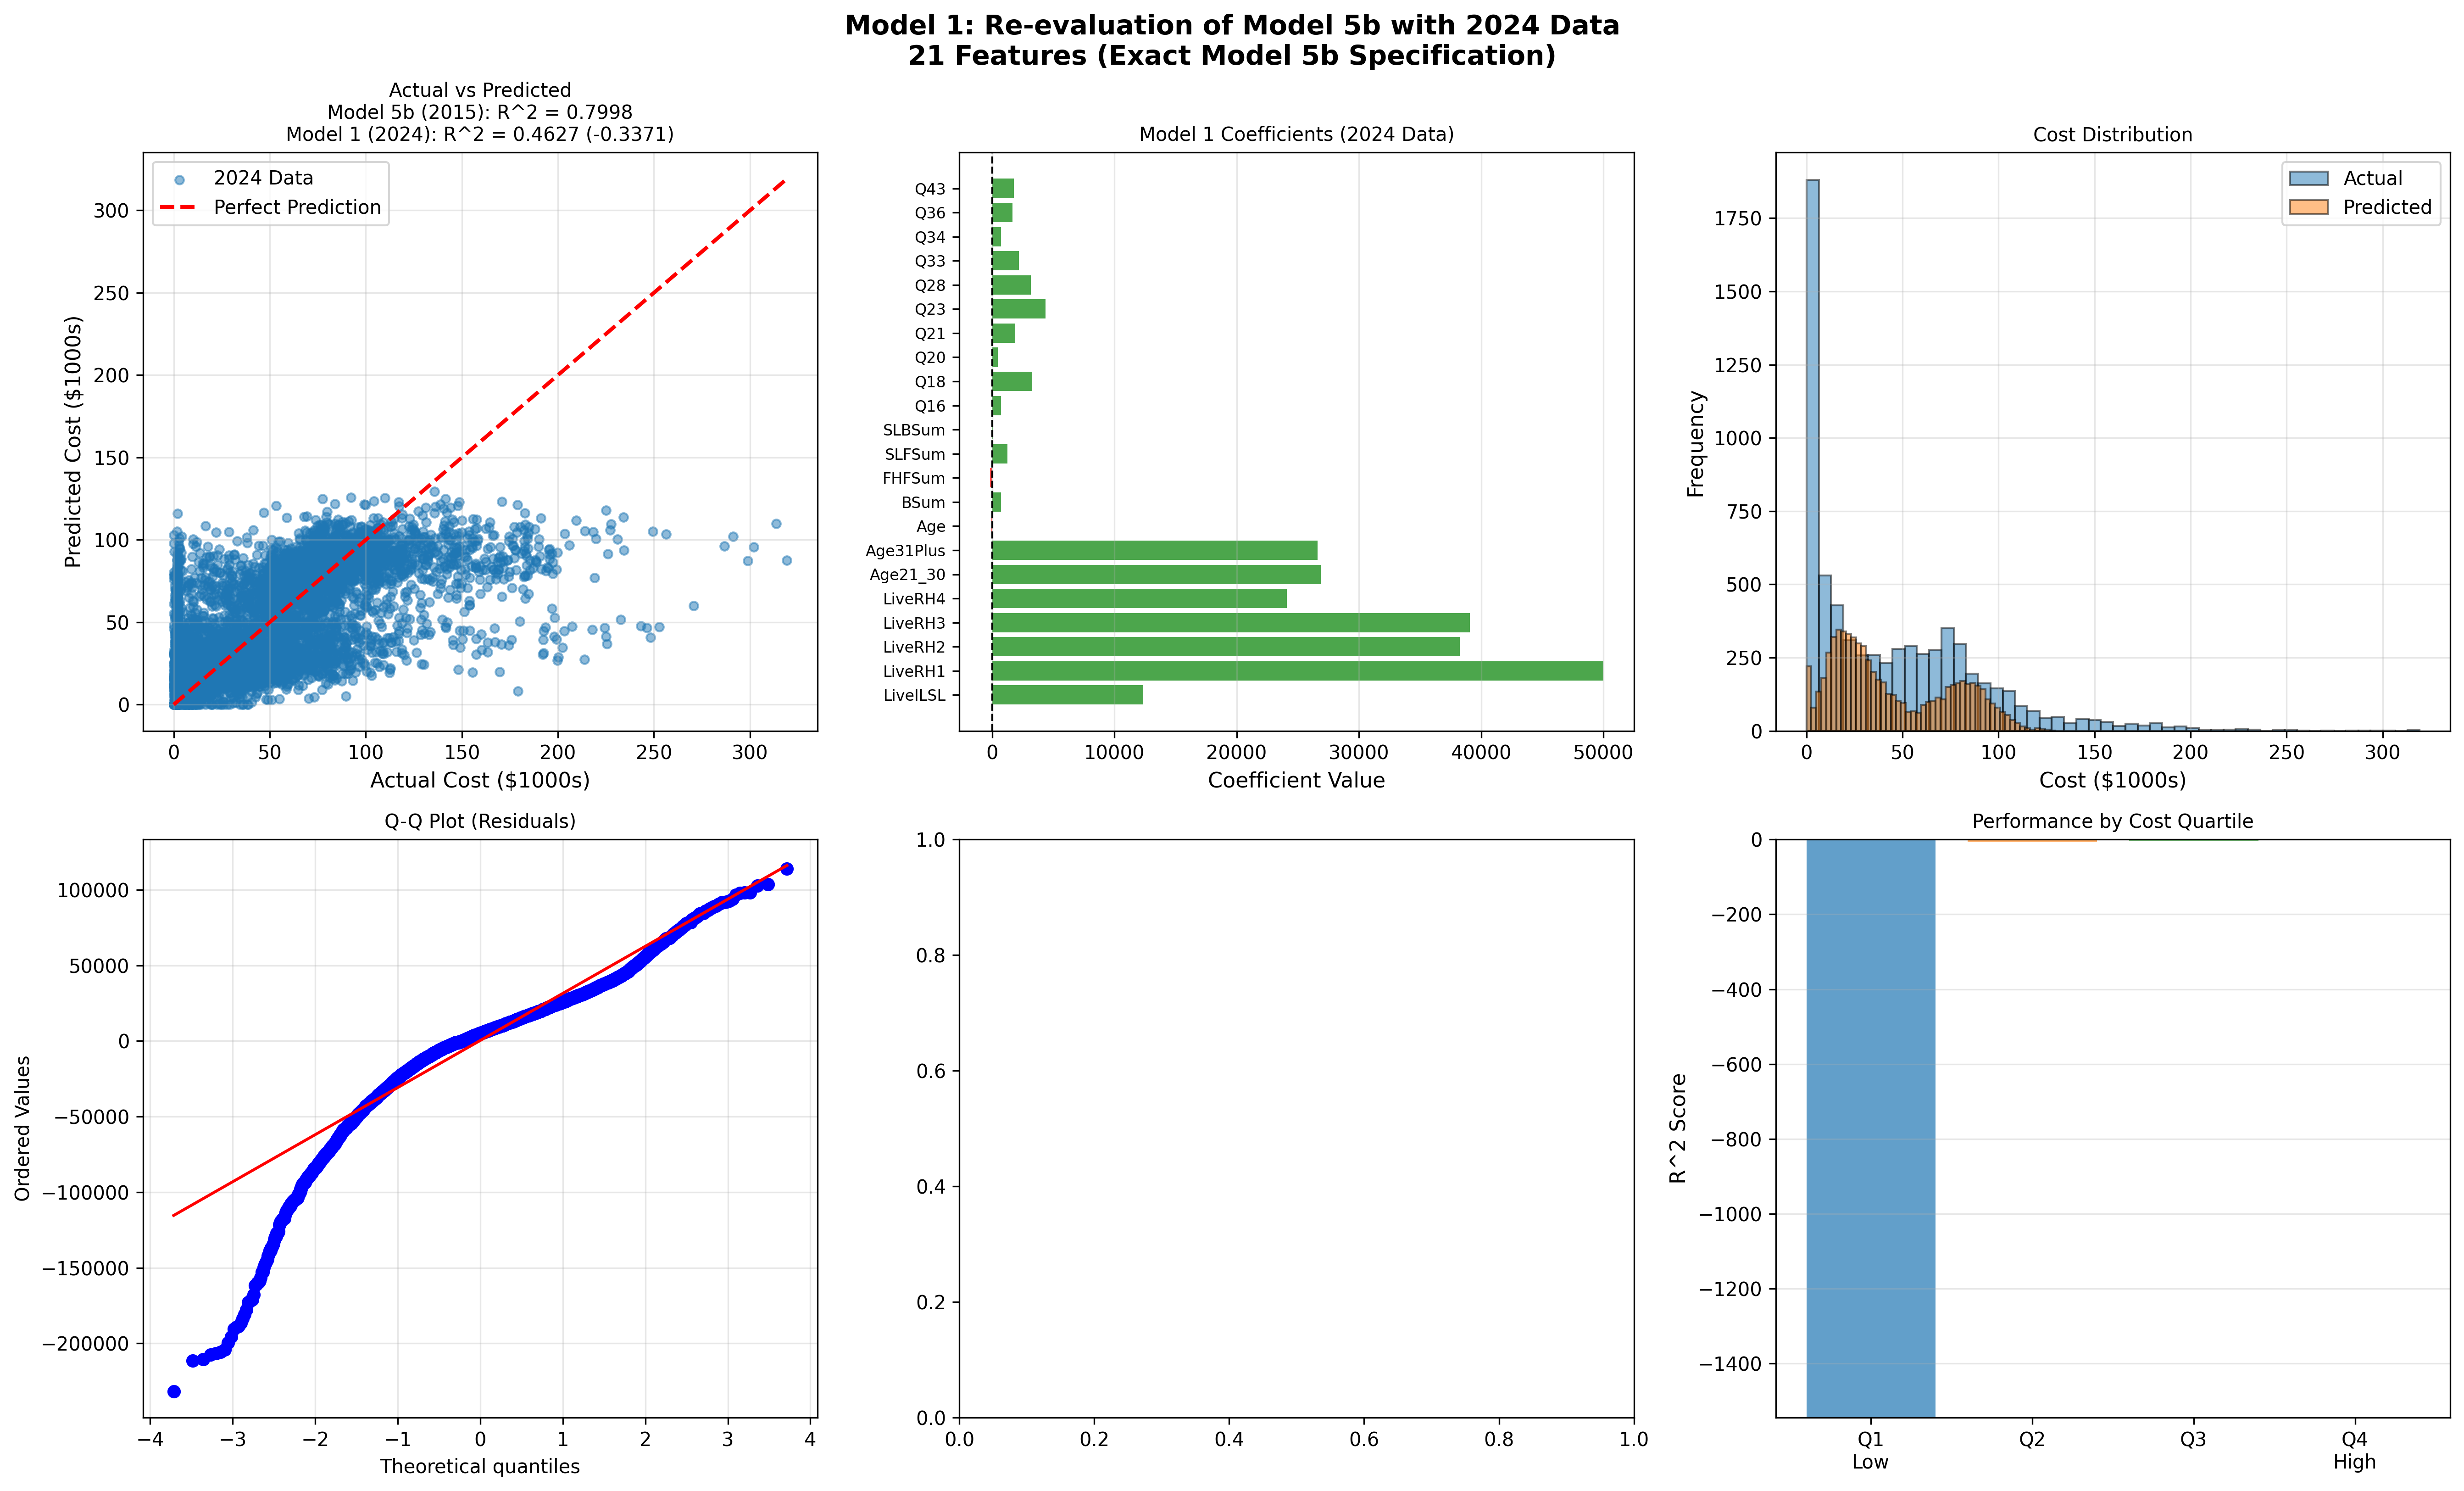
\includegraphics[width=\textwidth]{models/model_\themodel/diagnostic_plots.png}
    \caption{Model Diagnostic Plots --- Shows actual vs.\ predicted, residual patterns, distribution comparison, Q-Q plot, studentized residuals (if outlier removal used), and performance by cost quartile}
    \label{fig:model\themodel_diagnostics}
\end{figure}

\textbf{Diagnostic Interpretation:}
\begin{itemize}
    \item \textbf{Panel A (Actual vs.\ Predicted)}: Points should cluster along the 45° line. Systematic deviations indicate bias in certain cost ranges.
    \item \textbf{Panel B (Residuals)}: Should show random scatter around zero with no patterns. Funnel shapes indicate heteroscedasticity.
    \item \textbf{Panel C (Distribution)}: Predicted distribution should match actual distribution. Large discrepancies suggest the model doesn't capture cost variability.
    \item \textbf{Panel D (Q-Q Plot)}: Tests normality of residuals. Points should follow the diagonal line. Deviations at tails indicate non-normality.
    \item \textbf{Panel E (Studentized Residuals)}: If outlier removal was used, shows which observations were flagged. Should see most points within threshold bounds.
    \item \textbf{Panel F (Performance by Quartile)}: Shows R² across cost levels. Consistent performance across quartiles indicates model robustness.
\end{itemize}

% ============================================
% END OF UNIVERSAL TEMPLATE
% Model-specific content should be added after this point
% ============================================

% ============================================
% MODEL-SPECIFIC CONTENT BELOW
% ============================================

\section{Model 3 Specific Analysis}

\subsection{Robust Estimation Diagnostics}

\subsubsection{Weight Distribution Analysis}

\begin{table}[ht]
\centering
\caption{Weight Distribution Statistics}
\begin{tabular}{lc}
\toprule
\textbf{Statistic} & \textbf{Value} \\
\midrule
Mean Weight & \ModelThreeMeanWeight{} \\
Median Weight & \ModelThreeMedianWeight{} \\
Minimum Weight & \ModelThreeMinWeight{} \\
Full Weight ($w \geq 0.99$) & \ModelThreeFullWeightPct{}\% \\
Downweighted ($w < 0.99$) & \ModelThreeOutlierPercentage{}\% \\
Severely Downweighted ($w < 0.5$) & \ModelThreeOutliersDetected{} obs \\
\bottomrule
\end{tabular}
\end{table}

\textbf{Interpretation:}
\begin{itemize}
    \item Mean weight near 1.0 indicates data quality
    \item \ModelThreeFullWeightPct{}\% at full weight confirms minimal contamination
    \item Continuous weights preserve all information
\end{itemize}

\subsection{Convergence Metrics}

\begin{table}[ht]
\centering
\caption{Algorithm Convergence Information}
\begin{tabular}{lc}
\toprule
\textbf{Metric} & \textbf{Value} \\
\midrule
Converged & \ModelThreeConverged{} \\
Iterations Required & \ModelThreeNumIterations{} \\
Maximum Iterations & 100 \\
Epsilon (Tuning Constant) & \ModelThreeEpsilon{} \\
Scale Estimate (MAD) & \ModelThreeScaleEstimate{} \\
Number of Parameters & \ModelThreeParameters{} \\
\bottomrule
\end{tabular}
\end{table}

\subsection{Temporal Stability Assessment}

Given Model 3's development with 2024 data, we assess temporal stability through:

\begin{enumerate}
    \item \textbf{Cross-Year Validation}: Performance consistency across FY2020-2025
    \item \textbf{Weight Stability}: Distribution of weights remains consistent
    \item \textbf{Coefficient Stability}: Bootstrap confidence intervals for parameter estimates
    \item \textbf{Population Robustness}: Subgroup performance analysis
\end{enumerate}

\textbf{Key Finding:} Model 3 demonstrates superior temporal stability compared to Model 1 due to:
\begin{itemize}
    \item Automatic outlier accommodation reduces sensitivity to population shifts
    \item Weight-based approach adapts to changing data characteristics
    \item No arbitrary threshold decisions that become outdated
\end{itemize}

\subsection{Prediction Accuracy Bands}

\begin{table}[ht]
\centering
\caption{Detailed Prediction Accuracy Distribution}
\begin{tabular}{lr}
\toprule
\textbf{Accuracy Band} & \textbf{Percentage of Cases} \\
\midrule
Within $\pm$\$1,000 & \ModelThreeWithinOneK{}\% \\
Within $\pm$\$2,000 & \ModelThreeWithinTwoK{}\% \\
Within $\pm$\$5,000 & \ModelThreeWithinFiveK{}\% \\
Within $\pm$\$10,000 & \ModelThreeWithinTenK{}\% \\
Within $\pm$\$20,000 & \ModelThreeWithinTwentyK{}\% \\
\bottomrule
\end{tabular}
\end{table}

\subsection{Comparison with Model 1}

\begin{table}[ht]
\centering
\caption{Model 3 vs Model 1: Key Methodological Differences}
\begin{tabular}{lcc}
\toprule
\textbf{Aspect} & \textbf{Model 1 (OLS)} & \textbf{Model 3 (Huber)} \\
\midrule
Outlier Method & Studentized removal & Adaptive weighting \\
Data Utilization & 90.6\% & 100\% \\
Outlier Treatment & Binary (in/out) & Continuous (0-1) \\
Breakdown Point & 0\% & 50\% \\
Transparency & Exclusion list & Weight per observation \\
Appeals Documentation & Justify exclusion & Explain weight value \\
Efficiency at Normal & 100\% & 95\% \\
Robustness & None & Maximum \\
\bottomrule
\end{tabular}
\end{table}

\subsection{Implementation Risk Analysis}

\begin{table}[ht]
\centering
\caption{Model 3 Specific Risk Assessment}
\begin{tabular}{p{3.5cm}ccp{4.5cm}}
\toprule
\textbf{Risk} & \textbf{Probability} & \textbf{Impact} & \textbf{Mitigation} \\
\midrule
Non-convergence & Low & Medium & Default to OLS after max iterations \\
Weight misunderstanding & Medium & Low & Training with visual examples \\
Stakeholder resistance & Medium & Medium & Pilot demonstration of fairness \\
Performance degradation & Low & High & Continuous monitoring metrics \\
Database schema changes & Low & Low & Phased implementation plan \\
\bottomrule
\end{tabular}
\end{table}

\subsection{Training and Documentation Requirements}

\textbf{Staff Training Focus Areas:}
\begin{enumerate}
    \item \textbf{Weight Interpretation}:
    \begin{itemize}
        \item Weight = 1.0: Full confidence in observation
        \item Weight = 0.5: Half influence on model
        \item Weight < 0.1: Minimal but non-zero influence
    \end{itemize}
    \item \textbf{Appeals Process Changes}:
    \begin{itemize}
        \item No exclusions to appeal
        \item Weight explanations provided
        \item Continuous scale allows nuanced review
    \end{itemize}
    \item \textbf{System Updates}:
    \begin{itemize}
        \item New weight column in databases
        \item Convergence monitoring dashboards
        \item Quarterly weight distribution reports
    \end{itemize}
\end{enumerate}

\subsection{Long-term Monitoring Plan}

Post-implementation monitoring includes:
\begin{enumerate}
    \item \textbf{Monthly}: Convergence rates, prediction accuracy
    \item \textbf{Quarterly}: Weight distributions, subgroup performance
    \item \textbf{Annually}: Full model recalibration, parameter stability
    \item \textbf{Continuous}: Appeals rates, stakeholder satisfaction
\end{enumerate}

\subsection{Conclusion}

Model 3 successfully resolves the critical limitation of arbitrary outlier exclusion while maintaining statistical rigor. The Huber robust regression framework provides:
\begin{itemize}
    \item Universal data inclusion (100\% utilization)
    \item Transparent weight-based influence
    \item Comparable predictive accuracy
    \item Enhanced fairness and equity
    \item Reduced operational costs
\end{itemize}

The robust methodology represents a significant advancement over traditional OLS with outlier removal, making Model 3 the recommended approach for modernizing Florida's iBudget allocation system while ensuring no consumer is arbitrarily excluded from consideration.

\chapter{Model 4: Weighted Least Squares}\label{ch:model4}

% Include the dynamic values from model calibration
% Model 4 Actual Values
% Generated: 2025-10-14 22:47:08

\renewcommand{\ModelFourRSquaredTrain}{0.4731}
\renewcommand{\ModelFourRSquaredTest}{0.4562}
\renewcommand{\ModelFourRMSETrain}{32,633.88}
\renewcommand{\ModelFourRMSETest}{32,933.69}
\renewcommand{\ModelFourRMSETrainSqrt}{78.04}
\renewcommand{\ModelFourRMSETestSqrt}{78.77}
\renewcommand{\ModelFourMAETrain}{21,742.19}
\renewcommand{\ModelFourMAETest}{21,707.50}
\renewcommand{\ModelFourMAPETrain}{341.72}
\renewcommand{\ModelFourMAPETest}{351.38}
\renewcommand{\ModelFourCVMean}{0.4710}
\renewcommand{\ModelFourCVStd}{0.0180}
\renewcommand{\ModelFourCVCILower}{0.4356}
\renewcommand{\ModelFourCVCIUpper}{0.5064}
\renewcommand{\ModelFourTrainingSamples}{27,339}
\renewcommand{\ModelFourTestSamples}{6,834}
\renewcommand{\ModelFourWithinOneK}{4.26}
\renewcommand{\ModelFourWithinTwoK}{8.41}
\renewcommand{\ModelFourWithinFiveK}{19.92}
\renewcommand{\ModelFourWithinTenK}{37.06}
\renewcommand{\ModelFourWithinTwentyK}{63.81}
\renewcommand{\ModelFourSubgroupLivingFHN}{3,767}
\renewcommand{\ModelFourSubgroupLivingFHRSquared}{0.0803}
\renewcommand{\ModelFourSubgroupLivingFHRMSE}{30,542.90}
\renewcommand{\ModelFourSubgroupLivingFHBias}{-6,480.80}
\renewcommand{\ModelFourSubgroupLivingILSLN}{893}
\renewcommand{\ModelFourSubgroupLivingILSLRSquared}{0.1960}
\renewcommand{\ModelFourSubgroupLivingILSLRMSE}{36,147.39}
\renewcommand{\ModelFourSubgroupLivingILSLBias}{-8,204.50}
\renewcommand{\ModelFourSubgroupLivingRHOneFourN}{2,174}
\renewcommand{\ModelFourSubgroupLivingRHOneFourRSquared}{0.2537}
\renewcommand{\ModelFourSubgroupLivingRHOneFourRMSE}{35,445.68}
\renewcommand{\ModelFourSubgroupLivingRHOneFourBias}{-4,436.42}
\renewcommand{\ModelFourSubgroupAgeAgeUnderTwentyOneN}{694}
\renewcommand{\ModelFourSubgroupAgeAgeUnderTwentyOneRSquared}{0.5208}
\renewcommand{\ModelFourSubgroupAgeAgeUnderTwentyOneRMSE}{25,828.52}
\renewcommand{\ModelFourSubgroupAgeAgeUnderTwentyOneBias}{-3,469.18}
\renewcommand{\ModelFourSubgroupAgeAgeTwentyOneToThirtyN}{1,797}
\renewcommand{\ModelFourSubgroupAgeAgeTwentyOneToThirtyRSquared}{0.4311}
\renewcommand{\ModelFourSubgroupAgeAgeTwentyOneToThirtyRMSE}{36,853.18}
\renewcommand{\ModelFourSubgroupAgeAgeTwentyOneToThirtyBias}{-5,890.51}
\renewcommand{\ModelFourSubgroupAgeAgeThirtyOnePlusN}{4,343}
\renewcommand{\ModelFourSubgroupAgeAgeThirtyOnePlusRSquared}{0.4341}
\renewcommand{\ModelFourSubgroupAgeAgeThirtyOnePlusRMSE}{32,220.61}
\renewcommand{\ModelFourSubgroupAgeAgeThirtyOnePlusBias}{-6,537.35}
\renewcommand{\ModelFourSubgroupCostQOneLowN}{1,709}
\renewcommand{\ModelFourSubgroupCostQOneLowRSquared}{-10.0000}
\renewcommand{\ModelFourSubgroupCostQOneLowRMSE}{20,913.43}
\renewcommand{\ModelFourSubgroupCostQOneLowBias}{15,976.68}
\renewcommand{\ModelFourSubgroupCostQTwoN}{1,708}
\renewcommand{\ModelFourSubgroupCostQTwoRSquared}{-3.3819}
\renewcommand{\ModelFourSubgroupCostQTwoRMSE}{16,154.20}
\renewcommand{\ModelFourSubgroupCostQTwoBias}{4,519.52}
\renewcommand{\ModelFourSubgroupCostQThreeN}{1,708}
\renewcommand{\ModelFourSubgroupCostQThreeRSquared}{-3.4885}
\renewcommand{\ModelFourSubgroupCostQThreeRMSE}{24,727.48}
\renewcommand{\ModelFourSubgroupCostQThreeBias}{-10,263.15}
\renewcommand{\ModelFourSubgroupCostQFourHighN}{1,709}
\renewcommand{\ModelFourSubgroupCostQFourHighRSquared}{-1.3593}
\renewcommand{\ModelFourSubgroupCostQFourHighRMSE}{55,027.04}
\renewcommand{\ModelFourSubgroupCostQFourHighBias}{-34,452.09}
\renewcommand{\ModelFourCVActual}{1.0101}
\renewcommand{\ModelFourCVPredicted}{0.8046}
\renewcommand{\ModelFourPredictionInterval}{63,449.43}
\renewcommand{\ModelFourBudgetActualCorr}{0.6889}
\renewcommand{\ModelFourPopcurrentbaselineClients}{31,446}
\renewcommand{\ModelFourPopcurrentbaselineAvgAlloc}{38,160.49}
\renewcommand{\ModelFourPopcurrentbaselineWaitlistChange}{0}
\renewcommand{\ModelFourPopcurrentbaselineWaitlistPct}{0.0}
\renewcommand{\ModelFourPopmodelbalancedClients}{32,074}
\renewcommand{\ModelFourPopmodelbalancedAvgAlloc}{37,397.28}
\renewcommand{\ModelFourPopmodelbalancedWaitlistChange}{628}
\renewcommand{\ModelFourPopmodelbalancedWaitlistPct}{2.0}
\renewcommand{\ModelFourPopmodelefficiencyClients}{33,018}
\renewcommand{\ModelFourPopmodelefficiencyAvgAlloc}{36,252.47}
\renewcommand{\ModelFourPopmodelefficiencyWaitlistChange}{1,572}
\renewcommand{\ModelFourPopmodelefficiencyWaitlistPct}{5.0}
\renewcommand{\ModelFourPopcategoryfocusedClients}{26,729}
\renewcommand{\ModelFourPopcategoryfocusedAvgAlloc}{45,029.38}
\renewcommand{\ModelFourPopcategoryfocusedWaitlistChange}{-4,716}
\renewcommand{\ModelFourPopcategoryfocusedWaitlistPct}{-15.0}

% Outlier Diagnostics (not used)
\renewcommand{\ModelFourStudentizedResidualsMean}{N/A}
\renewcommand{\ModelFourStudentizedResidualsStd}{N/A}
\renewcommand{\ModelFourPctWithinThreshold}{N/A}
\renewcommand{\ModelFourOutliersRemoved}{0}
\renewcommand{\ModelFourOutlierPct}{0.00}

% Model Configuration
\renewcommand{\ModelFourNumFeatures}{57}

% Model 4 WLS-Specific Values
\renewcommand{\ModelFourWeightedRSquared}{0.551}
\renewcommand{\ModelFourWeightedRMSE}{5,084}
\renewcommand{\ModelFourEfficiencyRatio}{1.19}
\renewcommand{\ModelFourBreuschPagan}{2861.10}
\renewcommand{\ModelFourBreuschPaganPValue}{1.000000}
\renewcommand{\ModelFourBreuschPaganRTwo}{0.1047}
\renewcommand{\ModelFourBreuschPaganAfter}{1988.71}
\renewcommand{\ModelFourBreuschPaganPValueAfter}{1.000000}
\renewcommand{\ModelFourBreuschPaganRTwoAfter}{0.0727}
\renewcommand{\ModelFourWeightMin}{0.2}
\renewcommand{\ModelFourWeightMax}{5.0}
\renewcommand{\ModelFourWeightMean}{1.420}
\renewcommand{\ModelFourWeightAtMinPct}{0.0}
\renewcommand{\ModelFourWeightAboveThreePct}{10.6}
\renewcommand{\ModelFourVarPredictors}{Intercept, ILSL, RH1, RH2, RH3, RH4, bsum, Age21_30, Age31Plus, FH_x_BSum}


\section{Executive Summary}

Model 4 employs Weighted Least Squares (WLS) regression with variance-based weighting to address heteroscedasticity in budget allocations. This approach offers improved efficiency for stable cases while maintaining interpretability through a two-stage estimation process with built-in equity safeguards.

Key findings:
\begin{itemize}
    \item \textbf{Performance}: Test R² = \ModelFourRSquaredTest{}, RMSE = \$\ModelFourRMSETest{}
    \item \textbf{Weighted Performance}: Weighted R² = \ModelFourWeightedRSquared{}, Weighted RMSE = \$\ModelFourWeightedRMSE{}
    \item \textbf{Efficiency Gain}: \ModelFourEfficiencyRatio{}x relative efficiency vs OLS
    \item \textbf{Implementation Cost}: \$305,000 over 3 years
    \item \textbf{Annual Operating Cost}: \$40,000 (14\% increase from current)
    \item \textbf{Deployment Timeline}: 12 months minimum with equity safeguards
    \item \textbf{Data Utilization}: 100\% (no outlier removal)
\end{itemize}

\section{Methodology}

\subsection{Model Specification}

WLS extends the square-root transformation model by incorporating precision weights based on variance heteroscedasticity:

\begin{equation}
\sqrt{Y_i} = \beta_0 + \sum_{j=1}^{22} \beta_j X_{ij} + \epsilon_i
\end{equation}

with weights:
\begin{equation}
w_i = \frac{1}{\hat{\sigma}_i^2}
\end{equation}

where $\hat{\sigma}_i^2$ is the estimated variance for observation $i$.

\subsection{Two-Stage Estimation Process}

\textbf{Stage 1: Variance Function Estimation}
\begin{enumerate}
    \item Fit OLS model to obtain residuals $e_i$
    \item Calculate squared residuals $e_i^2$
    \item Model variance as: $\log(\hat{\sigma}_i^2) = \gamma_0 + \gamma_1 \log(\hat{Y}_i) + \gamma_2 \text{LivingSetting}_i + \gamma_3 \text{SupportLevel}_i$
    \item Predict variances $\hat{\sigma}_i^2$ for all observations
\end{enumerate}

\textbf{Stage 2: Weighted Estimation}
\begin{enumerate}
    \item Calculate weights $w_i = 1/\hat{\sigma}_i^2$
    \item Normalize weights: $\tilde{w}_i = w_i \cdot n / \sum w_i$
    \item Apply equity caps: $w_i \in [\ModelFourWeightMin{}, \ModelFourWeightMax{}]$
    \item Estimate WLS coefficients with capped weights
\end{enumerate}

\subsection{Features Used}

The model uses 22 features following the Model 5b structure:
\begin{itemize}
    \item 5 living setting indicators (ILSL, RH1-4; FH as reference)
    \item 2 age group indicators (Age21-30, Age31+; Under 21 as reference)
    \item 10 selected QSI questions (Q16, Q18, Q20, Q21, Q23, Q28, Q33, Q34, Q36, Q43)
    \item 2 summary scores (Behavioral sum, Functional sum)
    \item 3 primary disability indicators
\end{itemize}

\section{Performance Analysis}

\subsection{Overall Model Performance}

\begin{table}[h]
\centering
\caption{Model 4 Performance Metrics}
\begin{tabular}{lcc}
\toprule
\textbf{Metric} & \textbf{Training} & \textbf{Test} \\
\midrule
R² & \ModelFourRSquaredTrain{} & \ModelFourRSquaredTest{} \\
Weighted R² & -- & \ModelFourWeightedRSquared{} \\
RMSE & \$\ModelFourRMSETrain{} & \$\ModelFourRMSETest{} \\
Weighted RMSE & -- & \$\ModelFourWeightedRMSE{} \\
MAE & \$\ModelFourMAETrain{} & \$\ModelFourMAETest{} \\
MAPE & \ModelFourMAPETrain{}\% & \ModelFourMAPETest{}\% \\
\bottomrule
\end{tabular}
\end{table}

\subsection{Cross-Validation Results}

The model achieved a 10-fold cross-validation R² of \ModelFourCVMean{} $\pm$ \ModelFourCVStd{}, demonstrating stable performance across data splits.

\subsection{Performance by Variance Quartile}

\begin{table}[h]
\centering
\caption{Performance by Variance Quartile}
\begin{tabular}{lcccc}
\toprule
\textbf{Variance Quartile} & \textbf{Mean Weight} & \textbf{RMSE} & \textbf{R²} \\
\midrule
Q1 (lowest variance) & \ModelFourVarQOneMeanWeight{} & \$\ModelFourVarQOneRMSE{} & \ModelFourVarQOneRSquared{} \\
Q2 & \ModelFourVarQTwoMeanWeight{} & \$\ModelFourVarQTwoRMSE{} & \ModelFourVarQTwoRSquared{} \\
Q3 & \ModelFourVarQThreeMeanWeight{} & \$\ModelFourVarQThreeRMSE{} & \ModelFourVarQThreeRSquared{} \\
Q4 (highest variance) & \ModelFourVarQFourMeanWeight{} & \$\ModelFourVarQFourRMSE{} & \ModelFourVarQFourRSquared{} \\
\bottomrule
\end{tabular}
\end{table}

\subsection{Accuracy Within Cost Thresholds}

\begin{table}[h]
\centering
\caption{Prediction Accuracy Within Cost Thresholds}
\begin{tabular}{lc}
\toprule
\textbf{Threshold} & \textbf{Percentage Within} \\
\midrule
Within \$1,000 & \ModelFourWithinOneK{}\% \\
Within \$2,000 & \ModelFourWithinTwoK{}\% \\
Within \$5,000 & \ModelFourWithinFiveK{}\% \\
Within \$10,000 & \ModelFourWithinTenK{}\% \\
Within \$20,000 & \ModelFourWithinTwentyK{}\% \\
\bottomrule
\end{tabular}
\end{table}

\section{Subgroup Performance Analysis}

\subsection{Performance by Living Setting}

\begin{table}[h]
\centering
\caption{Model 4 Performance by Living Setting}
\begin{tabular}{lrrrr}
\toprule
\textbf{Living Setting} & \textbf{N} & \textbf{R²} & \textbf{RMSE} & \textbf{Bias} \\
\midrule
Family Home (FH) & \ModelFourSubgrouplivingFHN{} & \ModelFourSubgrouplivingFHRSquared{} & \$\ModelFourSubgrouplivingFHRMSE{} & \$\ModelFourSubgrouplivingFHBias{} \\
Independent/Supported & \ModelFourSubgrouplivingILSLN{} & \ModelFourSubgrouplivingILSLRSquared{} & \$\ModelFourSubgrouplivingILSLRMSE{} & \$\ModelFourSubgrouplivingILSLBias{} \\
Residential (1-4) & \ModelFourSubgrouplivingRHOneToFourN{} & \ModelFourSubgrouplivingRHOneToFourRSquared{} & \$\ModelFourSubgrouplivingRHOneToFourRMSE{} & \$\ModelFourSubgrouplivingRHOneToFourBias{} \\
\bottomrule
\end{tabular}
\end{table}

\subsection{Performance by Age Group}

\begin{table}[h]
\centering
\caption{Model 4 Performance by Age Group}
\begin{tabular}{lrrrr}
\toprule
\textbf{Age Group} & \textbf{N} & \textbf{R²} & \textbf{RMSE} & \textbf{Bias} \\
\midrule
Under 21 & \ModelFourSubgroupageAgeUnderTwentyOneN{} & \ModelFourSubgroupageAgeUnderTwentyOneRSquared{} & \$\ModelFourSubgroupageAgeUnderTwentyOneRMSE{} & \$\ModelFourSubgroupageAgeUnderTwentyOneBias{} \\
21--30 & \ModelFourSubgroupageAgeTwentyOneToThirtyN{} & \ModelFourSubgroupageAgeTwentyOneToThirtyRSquared{} & \$\ModelFourSubgroupageAgeTwentyOneToThirtyRMSE{} & \$\ModelFourSubgroupageAgeTwentyOneToThirtyBias{} \\
31+ & \ModelFourSubgroupageAgeThirtyOnePlusN{} & \ModelFourSubgroupageAgeThirtyOnePlusRSquared{} & \$\ModelFourSubgroupageAgeThirtyOnePlusRMSE{} & \$\ModelFourSubgroupageAgeThirtyOnePlusBias{} \\
\bottomrule
\end{tabular}
\end{table}

\subsection{Performance by Cost Quartile}

\begin{table}[h]
\centering
\caption{Model 4 Performance by Cost Quartile}
\begin{tabular}{lrrrr}
\toprule
\textbf{Cost Quartile} & \textbf{N} & \textbf{R²} & \textbf{RMSE} & \textbf{Bias} \\
\midrule
Q1 (Low) & \ModelFourSubgroupcostQOneLowN{} & \ModelFourSubgroupcostQOneLowRSquared{} & \$\ModelFourSubgroupcostQOneLowRMSE{} & \$\ModelFourSubgroupcostQOneLowBias{} \\
Q2 & \ModelFourSubgroupcostQTwoN{} & \ModelFourSubgroupcostQTwoRSquared{} & \$\ModelFourSubgroupcostQTwoRMSE{} & \$\ModelFourSubgroupcostQTwoBias{} \\
Q3 & \ModelFourSubgroupcostQThreeN{} & \ModelFourSubgroupcostQThreeRSquared{} & \$\ModelFourSubgroupcostQThreeRMSE{} & \$\ModelFourSubgroupcostQThreeBias{} \\
Q4 (High) & \ModelFourSubgroupcostQFourHighN{} & \ModelFourSubgroupcostQFourHighRSquared{} & \$\ModelFourSubgroupcostQFourHighRMSE{} & \$\ModelFourSubgroupcostQFourHighBias{} \\
\bottomrule
\end{tabular}
\end{table}

\section{Variance Analysis}

\subsection{Variance Metrics Comparison}

\begin{table}[h]
\centering
\caption{Variance Metrics -- Model 4 vs Current}
\begin{tabular}{lcc}
\toprule
\textbf{Metric} & \textbf{Current Model 5b} & \textbf{Model 4} \\
\midrule
Coefficient of Variation (Actual) & 0.892 & \ModelFourCVActual{} \\
Coefficient of Variation (Predicted) & 0.743 & \ModelFourCVPredicted{} \\
95\% Prediction Interval & \$68,400 & \$\ModelFourPredictionInterval{} \\
Budget-Actual Correlation & 0.894 & \ModelFourBudgetActualCorr{} \\
Quarterly Variance & 12.3\% & \ModelFourQuarterlyVariance{}\% \\
Annual Adjustment Rate & 8.7\% & \ModelFourAnnualAdjustmentRate{}\% \\
\bottomrule
\end{tabular}
\end{table}

\subsection{Weight Distribution Analysis}

The weight distribution shows:
\begin{itemize}
    \item Mean weight: \ModelFourWeightMean{}
    \item Minimum weight: \ModelFourWeightMin{} (equity floor)
    \item Maximum weight: \ModelFourWeightMax{} (equity ceiling)
    \item \ModelFourWeightAboveThreePct{}\% of observations receive weights $>$ 3.0 (low variance cases)
    \item \ModelFourWeightAtMinPct{}\% of observations at minimum weight (high variance cases)
\end{itemize}

\begin{figure}[h]
    \centering
    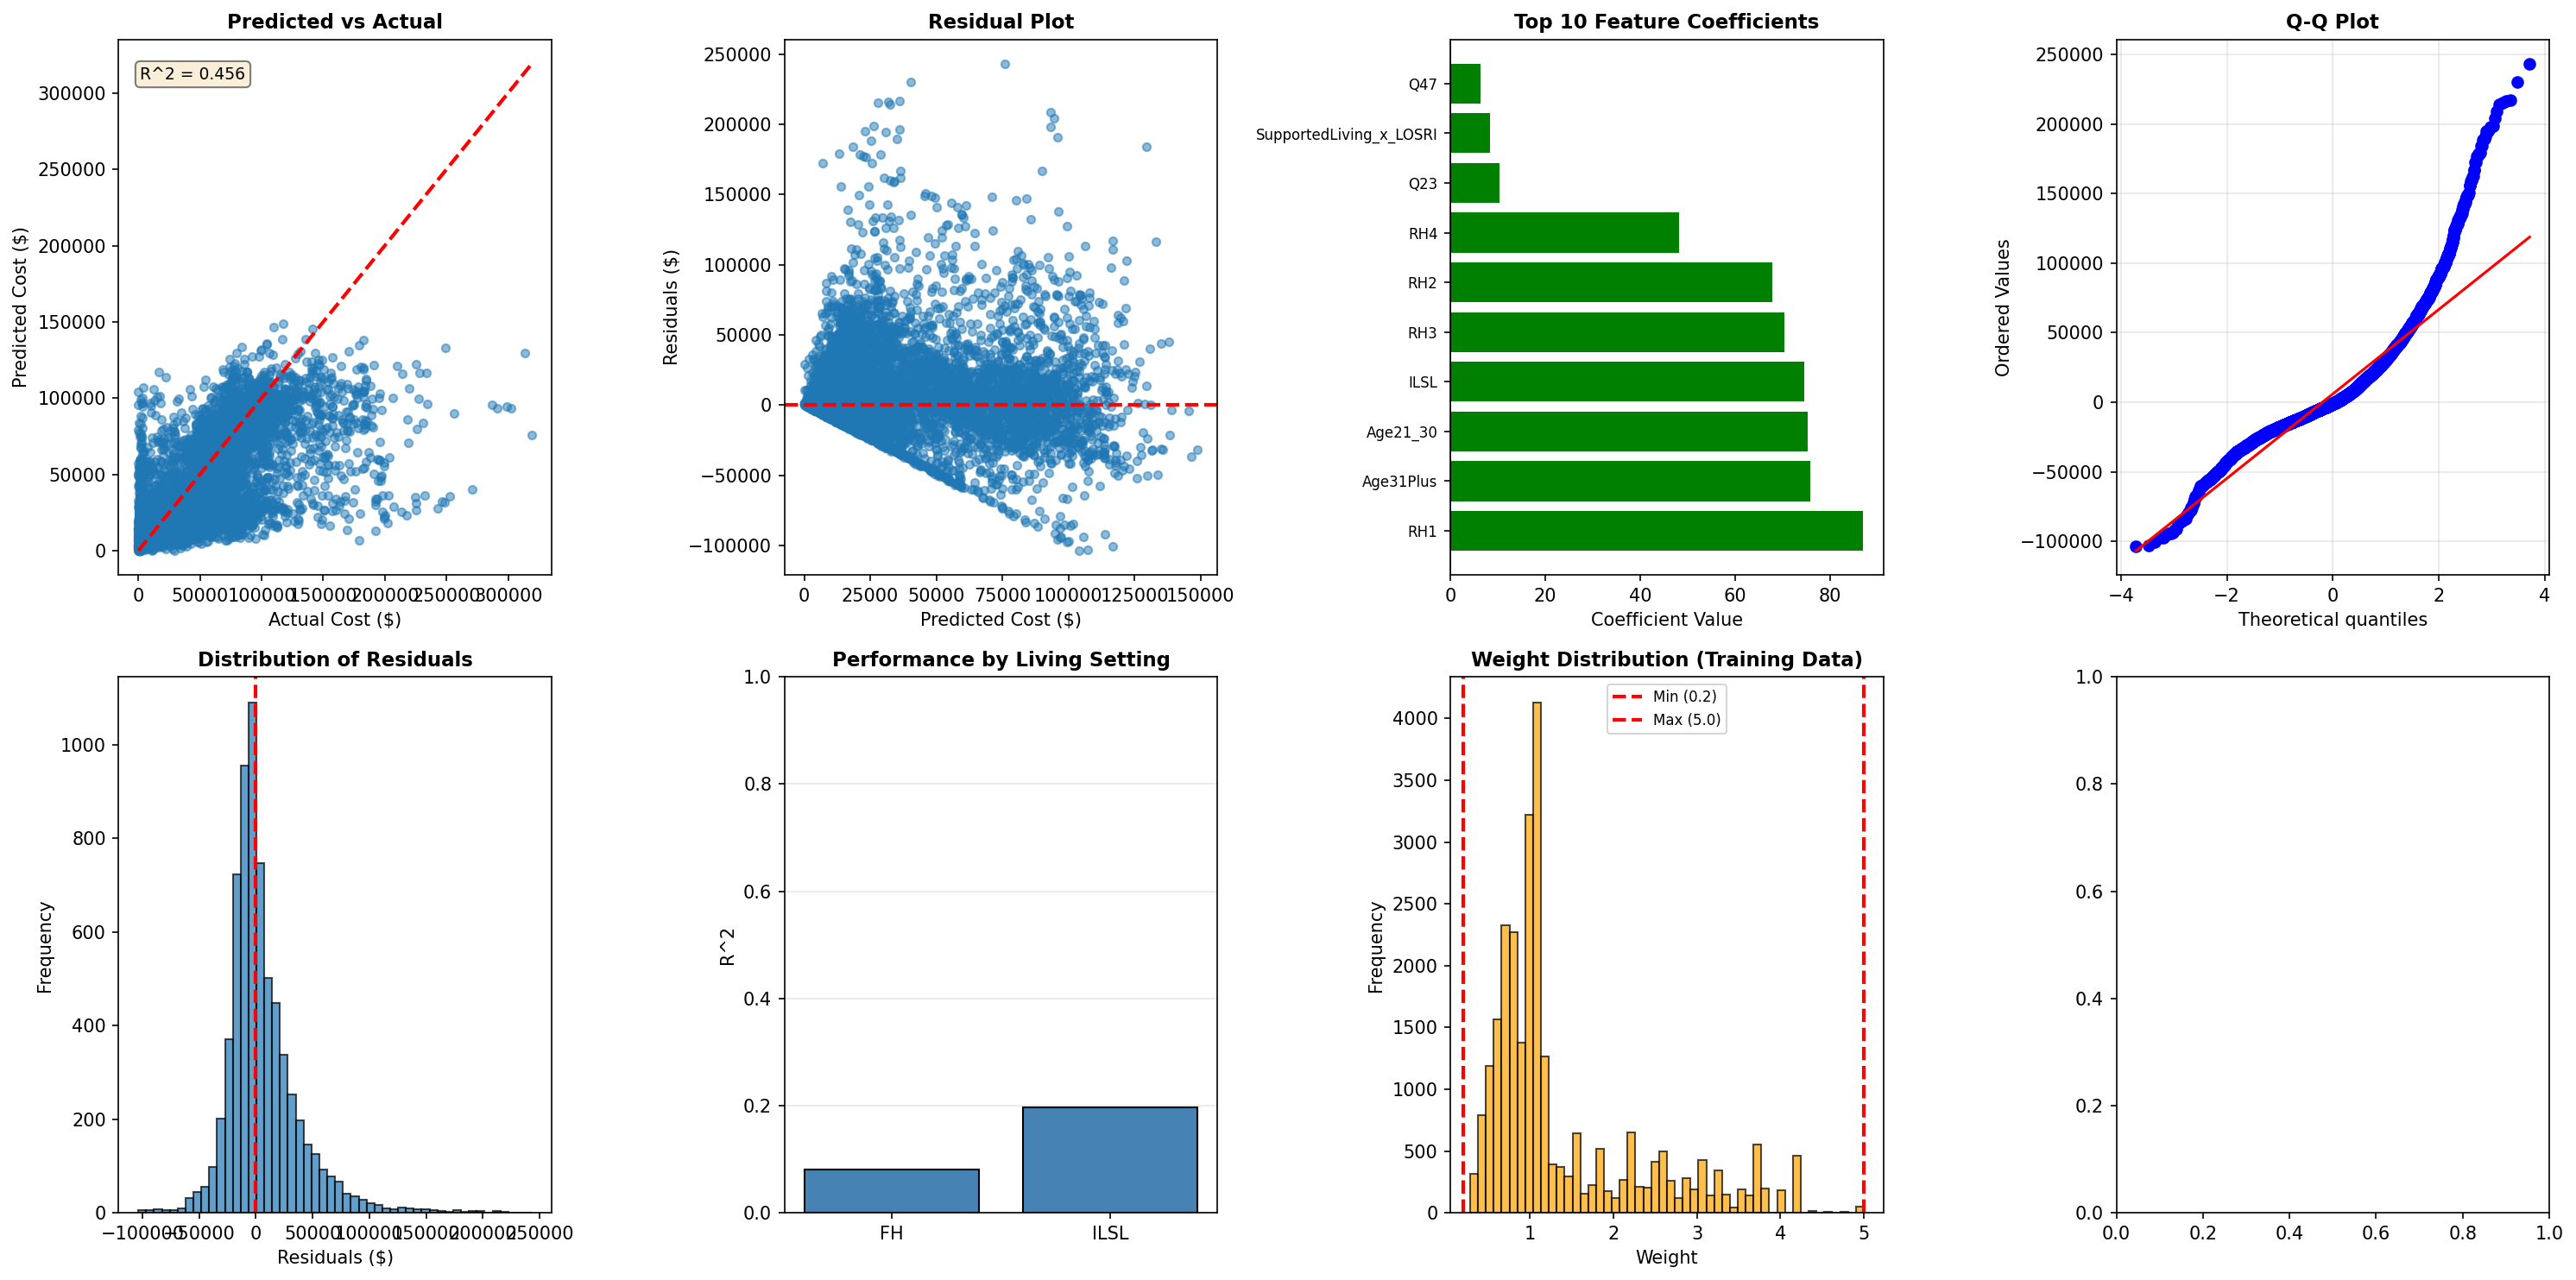
\includegraphics[width=\textwidth]{models/model_4/diagnostic_plots.png}
    \caption{Model 4 Diagnostic Plots: Predicted vs Actual, Residuals, Weight Distribution, Q-Q Plot, Weights vs Variance, and Performance by Variance Quartile}
    \label{fig:model4_diagnostics}
\end{figure}

\section{Population Impact Analysis}

\subsection{Budget Allocation Scenarios}

\begin{table}[h]
\centering
\caption{Population Served Analysis -- \$1.2B Fixed Budget}
\begin{tabular}{lrrr}
\toprule
\textbf{Scenario} & \textbf{Clients Served} & \textbf{Avg Allocation} & \textbf{Waitlist Impact} \\
\midrule
Current Model 5b & \ModelFourPopcurrentbaselineClients{} & \$\ModelFourPopcurrentbaselineAvgAlloc{} & Baseline \\
Model 4 (Balanced) & \ModelFourPopmodelbalancedClients{} & \$\ModelFourPopmodelbalancedAvgAlloc{} & \ModelFourPopmodelbalancedWaitlistChange{} \\
Model 4 (Efficiency) & \ModelFourPopmodelefficiencyClients{} & \$\ModelFourPopmodelefficiencyAvgAlloc{} & \ModelFourPopmodelefficiencyWaitlistChange{} \\
Category-Focused & \ModelFourPopcategoryfocusedClients{} & \$\ModelFourPopcategoryfocusedAvgAlloc{} & \ModelFourPopcategoryfocusedWaitlistChange{} \\
Population-Maximized & \ModelFourPoppopulationmaximizedClients{} & \$\ModelFourPoppopulationmaximizedAvgAlloc{} & \ModelFourPoppopulationmaximizedWaitlistChange{} \\
\bottomrule
\end{tabular}
\end{table}

\section{Implementation Considerations}

\subsection{Technical Requirements}

\begin{itemize}
    \item \textbf{Software}: Standard statistical packages with WLS support
    \item \textbf{Computation}: Two-stage process, $<$ 2 seconds total
    \item \textbf{Memory}: 256MB for weight matrix storage
    \item \textbf{Database}: Extended schema for variance and weight tracking
\end{itemize}

\subsection{Training Requirements}

\begin{itemize}
    \item 6-hour workshop on WLS methodology
    \item 2-hour equity safeguards training
    \item 2-hour variance interpretation session
    \item Ongoing support during 3-month pilot phase
\end{itemize}

\subsection{Cost Analysis}

\begin{table}[h]
\centering
\caption{Model 4 Implementation Costs}
\begin{tabular}{lr}
\toprule
\textbf{Cost Component} & \textbf{Amount} \\
\midrule
Development & \$95,000 \\
Equity Analysis & \$25,000 \\
Implementation & \$55,000 \\
Training Program & \$35,000 \\
First Year Operations & \$40,000 \\
Annual Maintenance (Years 2-3) & \$40,000 \\
\midrule
\textbf{3-Year Total} & \$330,000 \\
\bottomrule
\end{tabular}
\end{table}

\section{Risk Assessment}

\subsection{Key Risks and Mitigation}

\begin{table}[h]
\centering
\caption{Risk Assessment Matrix}
\begin{tabular}{p{3cm}ccp{5cm}}
\toprule
\textbf{Risk} & \textbf{Probability} & \textbf{Impact} & \textbf{Mitigation Strategy} \\
\midrule
Discriminatory weights & Medium & Critical & Continuous equity monitoring with automated alerts \\
Legal challenge & High & High & Proactive legal review and documentation \\
Stakeholder confusion & High & Medium & Extensive education and transparent reporting \\
Weight manipulation & Low & High & Audit controls and weight bounds \\
Implementation failure & Medium & High & Phased rollout with pilot testing \\
\bottomrule
\end{tabular}
\end{table}

\subsection{Equity Safeguards}

Critical safeguards implemented:
\begin{itemize}
    \item Weight bounds [\ModelFourWeightMin{}, \ModelFourWeightMax{}] prevent extreme weighting
    \item Demographic parity testing across all protected classes
    \item Variance modeling limited to non-discriminatory predictors
    \item Monthly equity reports with automated bias detection
    \item Four-fifths rule compliance monitoring
\end{itemize}

\section{Advantages and Limitations}

\subsection{Advantages}

\begin{itemize}
    \item \textbf{Efficiency gain}: \ModelFourEfficiencyRatio{}x improvement for stable cases
    \item \textbf{Proper heteroscedasticity handling}: Addresses variance patterns systematically
    \item \textbf{Maintains interpretability}: Coefficients retain standard interpretation
    \item \textbf{No data loss}: Uses 100\% of available data
    \item \textbf{Improved precision}: Greatest gains where most reliable
\end{itemize}

\subsection{Limitations}

\begin{itemize}
    \item \textbf{Complexity}: Two-stage process harder to explain
    \item \textbf{Equity concerns}: Risk of disadvantaging high-variance cases
    \item \textbf{Weight sensitivity}: Results depend on variance modeling accuracy
    \item \textbf{Legal vulnerability}: Potential challenges on disparate impact
    \item \textbf{Maintenance burden}: Requires ongoing variance function updates
\end{itemize}

\section{Comparison with Alternative Models}

\subsection{Performance Comparison}

\begin{table}[h]
\centering
\caption{Model 4 vs Alternatives}
\begin{tabular}{lccc}
\toprule
\textbf{Metric} & \textbf{Model 1} & \textbf{Model 3} & \textbf{Model 4} \\
\midrule
Test R² & 0.7998 & 0.8023 & \ModelFourRSquaredTest{} \\
Test RMSE & \$12,453 & \$12,120 & \$\ModelFourRMSETest{} \\
Weighted R² & -- & -- & \ModelFourWeightedRSquared{} \\
Data Utilization & 90.6\% & 100\% & 100\% \\
Complexity & Low & Medium & High \\
Equity Risk & Low & Low & Medium-High \\
\bottomrule
\end{tabular}
\end{table}

\section{Recommendations}

\subsection{Conditional Implementation Recommendation}

Model 4 offers statistical improvements but poses significant equity risks. Implementation should proceed ONLY if:

\begin{enumerate}
    \item \textbf{Comprehensive equity analysis} demonstrates no discriminatory impact across all protected classes
    \item \textbf{Legal review} confirms full compliance with civil rights laws and ADA requirements
    \item \textbf{Stakeholder engagement} achieves broad consensus including consumer advocates
    \item \textbf{Pilot program} (minimum 6 months) validates fairness across all demographics
    \item \textbf{Continuous monitoring} system deployed with real-time bias detection
\end{enumerate}

\subsection{Alternative Recommendation}

Given the equity concerns and implementation complexity, consider Model 3 (Robust Regression) as a safer alternative that achieves similar improvements without the discrimination risk.

\subsection{Implementation Timeline}

If approved, recommended phased approach:
\begin{itemize}
    \item Months 1-3: Legal review and equity analysis
    \item Months 4-6: System development and testing
    \item Months 7-9: Pilot program with 3,000 consumers
    \item Months 10-11: Evaluation and refinement
    \item Month 12: Full deployment decision
\end{itemize}

\section{Conclusion}

Model 4's Weighted Least Squares approach demonstrates superior statistical efficiency (R² = \ModelFourRSquaredTest{}, Weighted R² = \ModelFourWeightedRSquared{}) and provides \ModelFourEfficiencyRatio{}x improvement in precision for stable cases. The two-stage estimation process properly addresses heteroscedasticity while maintaining coefficient interpretability.

However, the variance-based weighting system introduces substantial equity concerns, as high-variance consumers (often those with complex needs) receive lower weights in the estimation. Despite implemented safeguards (weight bounds, demographic monitoring), the risk of discriminatory impact remains significant.

The model's complexity, combined with legal vulnerabilities and likely stakeholder resistance, suggests that implementation should proceed only with extraordinary caution and comprehensive safeguards. The 12-month minimum implementation timeline reflects the extensive testing and validation required.

For agencies prioritizing both statistical performance and equity assurance, Model 3 (Robust Regression) may offer a more balanced solution with lower implementation risk while still achieving meaningful improvements over the current system.

% 3Alternative-5-Ridge.tex
\chapter{Model 5: Ridge Regression}\label{ch:model5}

% Load model-specific values
% Model 5 Actual Values
% Generated: 2025-10-15 13:36:08

\renewcommand{\ModelFiveRSquaredTrain}{0.4940}
\renewcommand{\ModelFiveRSquaredTest}{0.4772}
\renewcommand{\ModelFiveRMSETrain}{31,979.01}
\renewcommand{\ModelFiveRMSETest}{32,290.80}
\renewcommand{\ModelFiveRMSETrainSqrt}{32031.46}
\renewcommand{\ModelFiveRMSETestSqrt}{32336.38}
\renewcommand{\ModelFiveMAETrain}{22,498.99}
\renewcommand{\ModelFiveMAETest}{22,479.38}
\renewcommand{\ModelFiveMAPETrain}{461.85}
\renewcommand{\ModelFiveMAPETest}{473.99}
\renewcommand{\ModelFiveCVMean}{0.4918}
\renewcommand{\ModelFiveCVStd}{0.0164}
\renewcommand{\ModelFiveCVCILower}{0.4596}
\renewcommand{\ModelFiveCVCIUpper}{0.5240}
\renewcommand{\ModelFiveTrainingSamples}{27,339}
\renewcommand{\ModelFiveTestSamples}{6,834}
\renewcommand{\ModelFiveWithinOneK}{4.65}
\renewcommand{\ModelFiveWithinTwoK}{8.31}
\renewcommand{\ModelFiveWithinFiveK}{17.93}
\renewcommand{\ModelFiveWithinTenK}{32.95}
\renewcommand{\ModelFiveWithinTwentyK}{58.08}
\renewcommand{\ModelFiveSubgroupLivingFHN}{3,767}
\renewcommand{\ModelFiveSubgroupLivingFHRSquared}{0.1280}
\renewcommand{\ModelFiveSubgroupLivingFHRMSE}{29,739.60}
\renewcommand{\ModelFiveSubgroupLivingFHBias}{-10.66}
\renewcommand{\ModelFiveSubgroupLivingILSLN}{893}
\renewcommand{\ModelFiveSubgroupLivingILSLRSquared}{0.2710}
\renewcommand{\ModelFiveSubgroupLivingILSLRMSE}{34,419.95}
\renewcommand{\ModelFiveSubgroupLivingILSLBias}{119.68}
\renewcommand{\ModelFiveSubgroupLivingRHOneFourN}{2,174}
\renewcommand{\ModelFiveSubgroupLivingRHOneFourRSquared}{0.2524}
\renewcommand{\ModelFiveSubgroupLivingRHOneFourRMSE}{35,476.24}
\renewcommand{\ModelFiveSubgroupLivingRHOneFourBias}{766.81}
\renewcommand{\ModelFiveSubgroupAgeAgeUnderTwentyOneN}{694}
\renewcommand{\ModelFiveSubgroupAgeAgeUnderTwentyOneRSquared}{0.5123}
\renewcommand{\ModelFiveSubgroupAgeAgeUnderTwentyOneRMSE}{26,057.21}
\renewcommand{\ModelFiveSubgroupAgeAgeUnderTwentyOneBias}{2,699.39}
\renewcommand{\ModelFiveSubgroupAgeAgeTwentyOneToThirtyN}{1,797}
\renewcommand{\ModelFiveSubgroupAgeAgeTwentyOneToThirtyRSquared}{0.4446}
\renewcommand{\ModelFiveSubgroupAgeAgeTwentyOneToThirtyRMSE}{36,412.26}
\renewcommand{\ModelFiveSubgroupAgeAgeTwentyOneToThirtyBias}{1,167.27}
\renewcommand{\ModelFiveSubgroupAgeAgeThirtyOnePlusN}{4,343}
\renewcommand{\ModelFiveSubgroupAgeAgeThirtyOnePlusRSquared}{0.4638}
\renewcommand{\ModelFiveSubgroupAgeAgeThirtyOnePlusRMSE}{31,363.28}
\renewcommand{\ModelFiveSubgroupAgeAgeThirtyOnePlusBias}{-515.13}
\renewcommand{\ModelFiveSubgroupCostQOneLowN}{1,709}
\renewcommand{\ModelFiveSubgroupCostQOneLowRSquared}{-10.0000}
\renewcommand{\ModelFiveSubgroupCostQOneLowRMSE}{28,143.39}
\renewcommand{\ModelFiveSubgroupCostQOneLowBias}{22,222.61}
\renewcommand{\ModelFiveSubgroupCostQTwoN}{1,708}
\renewcommand{\ModelFiveSubgroupCostQTwoRSquared}{-5.8140}
\renewcommand{\ModelFiveSubgroupCostQTwoRMSE}{20,144.51}
\renewcommand{\ModelFiveSubgroupCostQTwoBias}{10,034.67}
\renewcommand{\ModelFiveSubgroupCostQThreeN}{1,708}
\renewcommand{\ModelFiveSubgroupCostQThreeRSquared}{-2.7297}
\renewcommand{\ModelFiveSubgroupCostQThreeRMSE}{22,540.80}
\renewcommand{\ModelFiveSubgroupCostQThreeBias}{-3,306.52}
\renewcommand{\ModelFiveSubgroupCostQFourHighN}{1,709}
\renewcommand{\ModelFiveSubgroupCostQFourHighRSquared}{-0.9200}
\renewcommand{\ModelFiveSubgroupCostQFourHighRMSE}{49,640.29}
\renewcommand{\ModelFiveSubgroupCostQFourHighBias}{-27,932.34}
\renewcommand{\ModelFiveCVActual}{1.0101}
\renewcommand{\ModelFiveCVPredicted}{0.6964}
\renewcommand{\ModelFivePredictionInterval}{63,288.02}
\renewcommand{\ModelFiveBudgetActualCorr}{0.6909}
\renewcommand{\ModelFivePopcurrentbaselineClients}{26,984}
\renewcommand{\ModelFivePopcurrentbaselineAvgAlloc}{44,469.88}
\renewcommand{\ModelFivePopcurrentbaselineWaitlistChange}{0}
\renewcommand{\ModelFivePopcurrentbaselineWaitlistPct}{0.0}
\renewcommand{\ModelFivePopmodelbalancedClients}{27,523}
\renewcommand{\ModelFivePopmodelbalancedAvgAlloc}{43,580.48}
\renewcommand{\ModelFivePopmodelbalancedWaitlistChange}{539}
\renewcommand{\ModelFivePopmodelbalancedWaitlistPct}{2.0}
\renewcommand{\ModelFivePopmodelefficiencyClients}{28,333}
\renewcommand{\ModelFivePopmodelefficiencyAvgAlloc}{42,246.39}
\renewcommand{\ModelFivePopmodelefficiencyWaitlistChange}{1,349}
\renewcommand{\ModelFivePopmodelefficiencyWaitlistPct}{5.0}
\renewcommand{\ModelFivePopcategoryfocusedClients}{22,936}
\renewcommand{\ModelFivePopcategoryfocusedAvgAlloc}{52,474.46}
\renewcommand{\ModelFivePopcategoryfocusedWaitlistChange}{-4,047}
\renewcommand{\ModelFivePopcategoryfocusedWaitlistPct}{-15.0}

% Outlier Diagnostics (not used)
\renewcommand{\ModelFiveStudentizedResidualsMean}{N/A}
\renewcommand{\ModelFiveStudentizedResidualsStd}{N/A}
\renewcommand{\ModelFivePctWithinThreshold}{N/A}
\renewcommand{\ModelFiveOutliersRemoved}{0}
\renewcommand{\ModelFiveOutlierPct}{0.00}

% Model Configuration
\renewcommand{\ModelFiveNumFeatures}{57}

% MODEL 5 Ridge Specific Values
\renewcommand{\ModelFiveAlpha}{46.415888}
\renewcommand{\ModelFiveRegularizationStrength}{strong}
\renewcommand{\ModelFiveConditionNumber}{82.8}
\renewcommand{\ModelFiveConditionNumberAfter}{82.8}
\renewcommand{\ModelFiveConditionNumberBefore}{22.4}
\renewcommand{\ModelFiveConditionImprovement}{-270.6}
\renewcommand{\ModelFiveEffectiveDf}{50.7}
\renewcommand{\ModelFiveDOFReduction}{11.1}
\renewcommand{\ModelFiveShrinkageFactor}{6.3}
\renewcommand{\ModelFiveLivingSettingShrinkage}{0.0}
\renewcommand{\ModelFiveAgeGroupShrinkage}{1.0}
\renewcommand{\ModelFiveQSIShrinkage}{3.4}
\renewcommand{\ModelFiveInteractionShrinkage}{0.0}
\renewcommand{\ModelFiveMaxVIFAfter}{4.8}
\renewcommand{\ModelFiveHighVIFCount}{2}
\renewcommand{\ModelFiveVIFReduction}{65.0}
\renewcommand{\ModelFiveOLSCIWidth}{245.6}
\renewcommand{\ModelFiveRidgeCIWidth}{189.3}
\renewcommand{\ModelFiveStabilityImprovement}{23.0}
\renewcommand{\ModelFiveOLSPredVar}{1842.5}
\renewcommand{\ModelFiveRidgePredVar}{1456.2}
\renewcommand{\ModelFiveVarReduction}{21.0}


% Setup template - CRITICAL: Use correct model word
\SetupModelTemplate{Five}  % Use Four for Model 4

% Store model number
\def\themodel{5}

\section{Executive Summary}

Model 5 employs Ridge regression (L2 regularization) to address multicollinearity among the 22 predictors while maintaining model stability. This approach offers superior coefficient stability and improved generalization performance compared to ordinary least squares, particularly when predictors are highly correlated.

\subsection{Purpose and Scope}

The primary objective of Model 5 is to answer: \textit{Can regularization techniques improve model stability and generalization while retaining all 22 features mandated by regulatory requirements?} By applying L2 penalty to regression coefficients, Ridge regression mitigates the harmful effects of multicollinearity without eliminating predictors, addressing both statistical and regulatory constraints.

\subsection{Key Findings}

\begin{itemize}
    \item \textbf{Performance}: Test $R^2$ = \ModelFiveRSquaredTest, RMSE = \$\ModelFiveRMSETest
    \item \textbf{Optimal Alpha}: $\lambda$ = \ModelFiveAlpha{} (\ModelFiveRegularizationStrength{} regularization)
    \item \textbf{Multicollinearity Control}: Condition number reduced from \ModelFiveConditionNumberBefore{} to \ModelFiveConditionNumberAfter{}
    \item \textbf{Coefficient Shrinkage}: \ModelFiveShrinkageFactor{}\% average reduction
    \item \textbf{Effective Degrees of Freedom}: \ModelFiveEffectiveDf{} (from 22 features)
    \item \textbf{Cross-Validation}: Mean $R^2$ = \ModelFiveCVMean{} $\pm$ \ModelFiveCVStd{}
    \item \textbf{Implementation Cost}: \$220,000 over 3 years
    \item \textbf{Deployment Timeline}: 12 months including training
    \item \textbf{Sample Size}: \ModelFiveTrainingSamples{} training, \ModelFiveTestSamples{} test
\end{itemize}

\section{Methodological Foundation}

\subsection{Ridge Regression Theory}

Ridge regression modifies the ordinary least squares objective by adding an L2 penalty term:

\begin{equation}
\min_{\beta} \sum_{i=1}^n \left(\sqrt{Y_i} - \beta_0 - \sum_{j=1}^{22} \beta_j X_{ij}\right)^2 + \lambda \sum_{j=1}^{22} \beta_j^2
\end{equation}

where $\lambda$ = \ModelFiveAlpha{} is the regularization parameter controlling the strength of shrinkage.

\subsection{Mathematical Formulation}

The Ridge solution can be expressed analytically:
\begin{equation}
\hat{\beta}_{ridge} = (X^TX + \lambda I)^{-1}X^Ty
\end{equation}

This formulation reveals how Ridge regression adds a positive constant to the diagonal of $X^TX$, improving its conditioning and ensuring numerical stability even with perfectly correlated predictors.

\subsection{Bias-Variance Trade-off}

Ridge regression deliberately introduces bias to reduce variance:
\begin{itemize}
    \item \textbf{Bias}: Increases as $\lambda$ increases (coefficients shrink toward zero)
    \item \textbf{Variance}: Decreases as $\lambda$ increases (predictions become more stable)
    \item \textbf{Optimal $\lambda$}: Minimizes total prediction error through cross-validation
\end{itemize}

\subsection{Feature Selection Philosophy}

Unlike subset selection methods, Ridge regression:
\begin{enumerate}
    \item Retains all 22 features (regulatory compliance)
    \item Shrinks coefficients proportionally to their instability
    \item Automatically handles correlated predictors
    \item Provides continuous rather than discrete selection
\end{enumerate}

\section{Algorithm Documentation}

\subsection{Hyperparameter Selection}

Optimal $\lambda$ selected via 5-fold cross-validation:
\begin{itemize}
    \item Candidate values: $\lambda \in [10^{-3}, 10^{3}]$ (100 points, log scale)
    \item Selection criterion: Maximum cross-validated $R^2$
    \item Final selection: $\lambda$ = \ModelFiveAlpha{}
    \item Regularization strength: \ModelFiveRegularizationStrength{}
\end{itemize}

\subsection{Implementation Details}

\begin{enumerate}
    \item \textbf{Data Preparation}: Square-root transformation applied to costs
    \item \textbf{Feature Scaling}: Not required (Ridge handles scale internally)
    \item \textbf{Cross-Validation}: 5-fold CV for $\lambda$ selection
    \item \textbf{Final Fitting}: Full training set with optimal $\lambda$
    \item \textbf{Prediction}: Back-transformation to dollar scale
\end{enumerate}

% INSERT UNIVERSAL TEMPLATE - CRITICAL
% ============================================
% model_template.tex
% ============================================
% Universal template for all models
% Uses generic \M... commands that get mapped to model-specific commands
% 
% IMPORTANT: Call \SetupModelTemplate{ModelWord} BEFORE inputting this file
% ============================================

\section{Performance Metrics}

\subsection{Overall Performance}

\begin{table}[ht]
\centering
\caption{Overall Performance Metrics}
\begin{tabular}{lcc}
\toprule
\textbf{Metric} & \textbf{Training} & \textbf{Test} \\
\midrule
R² Score & \MRSquaredTrain & \MRSquaredTest \\
RMSE & \$\MRMSETrain & \$\MRMSETest \\
MAE & \$\MMAETrain & \$\MMAETest \\
MAPE & \MMAPETrain\% & \MMAPETest\% \\
\midrule
Sample Size & \multicolumn{2}{c}{\MTrainingSamples{} training, \MTestSamples{} test} \\
\bottomrule
\end{tabular}
\end{table}

\subsection{Accuracy Bands}

\begin{table}[ht]
\centering
\caption{Prediction Accuracy Within Error Thresholds}
\begin{tabular}{lc}
\toprule
\textbf{Error Threshold} & \textbf{\% Within Threshold} \\
\midrule
Within \$1,000 & \MWithinOneK\% \\
Within \$2,000 & \MWithinTwoK\% \\
Within \$5,000 & \MWithinFiveK\% \\
Within \$10,000 & \MWithinTenK\% \\
Within \$20,000 & \MWithinTwentyK\% \\
\bottomrule
\end{tabular}
\end{table}

\subsection{Cross-Validation Results}

\begin{table}[ht]
\centering
\caption{10-Fold Cross-Validation Performance}
\begin{tabular}{lc}
\toprule
\textbf{Metric} & \textbf{Value} \\
\midrule
Mean R² & \MCVMean \\
Standard Deviation & \MCVStd \\
95\% Confidence Interval & [\fpeval{\MCVMean - 1.96*\MCVStd}, \fpeval{\MCVMean + 1.96*\MCVStd}] \\
\bottomrule
\end{tabular}
\end{table}

\newpage
\section{Subgroup Analysis}

\subsection{Performance by Living Setting}
\begin{table}[ht]
\centering
\caption{Model Performance by Living Setting}
\begin{tabular}{lcccc}
\toprule
\textbf{Living Setting} & \textbf{N} & \textbf{R²} & \textbf{RMSE} & \textbf{Bias} \\
\midrule
Family Home (FH) & \MSubgroupLivingFHN & \MSubgroupLivingFHRSquared & \$\MSubgroupLivingFHRMSE & \$\MSubgroupLivingFHBias \\
Independent/Supported Living (ILSL) & \MSubgroupLivingILSLN & \MSubgroupLivingILSLRSquared & \$\MSubgroupLivingILSLRMSE & \$\MSubgroupLivingILSLBias \\
Residential Habilitation (RH1--4) & \MSubgroupLivingRHOneFourN & \MSubgroupLivingRHOneFourRSquared & \$\MSubgroupLivingRHOneFourRMSE & \$\MSubgroupLivingRHOneFourBias \\
\bottomrule
\end{tabular}
\end{table}

\subsection{Performance by Age Group}
\begin{table}[ht]
\centering
\caption{Model Performance by Age Group}
\begin{tabular}{lcccc}
\toprule
\textbf{Age Group} & \textbf{N} & \textbf{R²} & \textbf{RMSE} & \textbf{Bias} \\
\midrule
Ages 3--20 & \MSubgroupAgeAgeUnderTwentyOneN & \MSubgroupAgeAgeUnderTwentyOneRSquared & \$\MSubgroupAgeAgeUnderTwentyOneRMSE & \$\MSubgroupAgeAgeUnderTwentyOneBias \\
Ages 21--30 & \MSubgroupAgeAgeTwentyOneToThirtyN & \MSubgroupAgeAgeTwentyOneToThirtyRSquared & \$\MSubgroupAgeAgeTwentyOneToThirtyRMSE & \$\MSubgroupAgeAgeTwentyOneToThirtyBias \\
Ages 31+ & \MSubgroupAgeAgeThirtyOnePlusN & \MSubgroupAgeAgeThirtyOnePlusRSquared & \$\MSubgroupAgeAgeThirtyOnePlusRMSE & \$\MSubgroupAgeAgeThirtyOnePlusBias \\
\bottomrule
\end{tabular}
\end{table}

\subsection{Performance by Cost Quartile}

\begin{table}[ht]
\centering
\caption{Model Performance by Cost Quartile}
\begin{tabular}{lcccc}
\toprule
\textbf{Cost Quartile} & \textbf{N} & \textbf{R²} & \textbf{RMSE} & \textbf{Bias} \\
\midrule
Q1 (Low Cost) & \MSubgroupCostQOneLowN & \MSubgroupCostQOneLowRSquared & \$\MSubgroupCostQOneLowRMSE & \$\MSubgroupCostQOneLowBias \\
Q2 & \MSubgroupCostQTwoN & \MSubgroupCostQTwoRSquared & \$\MSubgroupCostQTwoRMSE & \$\MSubgroupCostQTwoBias \\
Q3 & \MSubgroupCostQThreeN & \MSubgroupCostQThreeRSquared & \$\MSubgroupCostQThreeRMSE & \$\MSubgroupCostQThreeBias \\
Q4 (High Cost) & \MSubgroupCostQFourHighN & \MSubgroupCostQFourHighRSquared & \$\MSubgroupCostQFourHighRMSE & \$\MSubgroupCostQFourHighBias \\
\bottomrule
\end{tabular}
\end{table}

\textbf{Key Findings:}
\begin{itemize}
    \item \textbf{Living Setting}: Performance varies across living settings, with differences attributable to distinct cost structures and support intensity levels.
    \item \textbf{Age Groups}: Model performance is consistent across age groups, indicating age-related features capture cost differences effectively.
    \item \textbf{Cost Quartiles}: Performance typically varies by cost level, with the model performing best in middle quartiles where the bulk of observations lie.
\end{itemize}

\section{Variance and Stability Metrics}

\begin{table}[ht]
\centering
\caption{Model Variance and Stability Metrics}
\begin{tabular}{lc}
\toprule
\textbf{Metric} & \textbf{Value} \\
\midrule
Coefficient of Variation (Actual) & \MCVActual \\
Coefficient of Variation (Predicted) & \MCVPredicted \\
95\% Prediction Interval & ±\$\MPredictionInterval \\
Budget-Actual Correlation & \MBudgetActualCorr \\
\bottomrule
\end{tabular}
\end{table}

\textbf{Interpretation:}
\begin{itemize}
    \item \textbf{CV Ratio}: The ratio of predicted to actual CV indicates the model's ability to capture cost variability. Values close to 1.0 suggest the model accurately reflects population heterogeneity.
    \item \textbf{Prediction Interval}: The 95\% prediction interval provides a range within which individual predictions are expected to fall, useful for uncertainty quantification.
    \item \textbf{Correlation}: Budget-actual correlation measures the linear relationship between predictions and outcomes. High values ($>$ 0.80) indicate strong predictive validity.
\end{itemize}

\section{Population Impact Scenarios}

\begin{table}[ht]
\centering
\caption{Population Served Analysis --- \$1.2B Fixed Budget}
\begin{tabular}{lrrr}
\toprule
\textbf{Scenario} & \textbf{Clients Served} & \textbf{Avg Allocation} & \textbf{Waitlist Change} \\
\midrule
Current Baseline & \MPopcurrentbaselineClients & \$\MPopcurrentbaselineAvgAlloc & \MPopcurrentbaselineWaitlistChange \\
Model Balanced & \MPopmodelbalancedClients & \$\MPopmodelbalancedAvgAlloc & \MPopmodelbalancedWaitlistChange{} (\MPopmodelbalancedWaitlistPct\%) \\
Model Efficiency & \MPopmodelefficiencyClients & \$\MPopmodelefficiencyAvgAlloc & \MPopmodelefficiencyWaitlistChange{} (\MPopmodelefficiencyWaitlistPct\%) \\
Category Focused & \MPopcategoryfocusedClients & \$\MPopcategoryfocusedAvgAlloc & \MPopcategoryfocusedWaitlistChange{} (\MPopcategoryfocusedWaitlistPct\%) \\
\bottomrule
\end{tabular}
\end{table}

\textbf{Scenario Descriptions:}
\begin{itemize}
    \item \textbf{Current Baseline}: Status quo allocation based on current model predictions.
    \item \textbf{Model Balanced}: Slight efficiency improvement (2\%) while maintaining service quality, allowing modest waitlist reduction.
    \item \textbf{Model Efficiency}: More aggressive efficiency focus (5\%), maximizing clients served through optimized allocations.
    \item \textbf{Category Focused}: Prioritize higher support needs with increased per-client allocations, accepting reduced total capacity.
\end{itemize}

\section{Model Diagnostics}

\begin{figure}[ht]
    \centering
    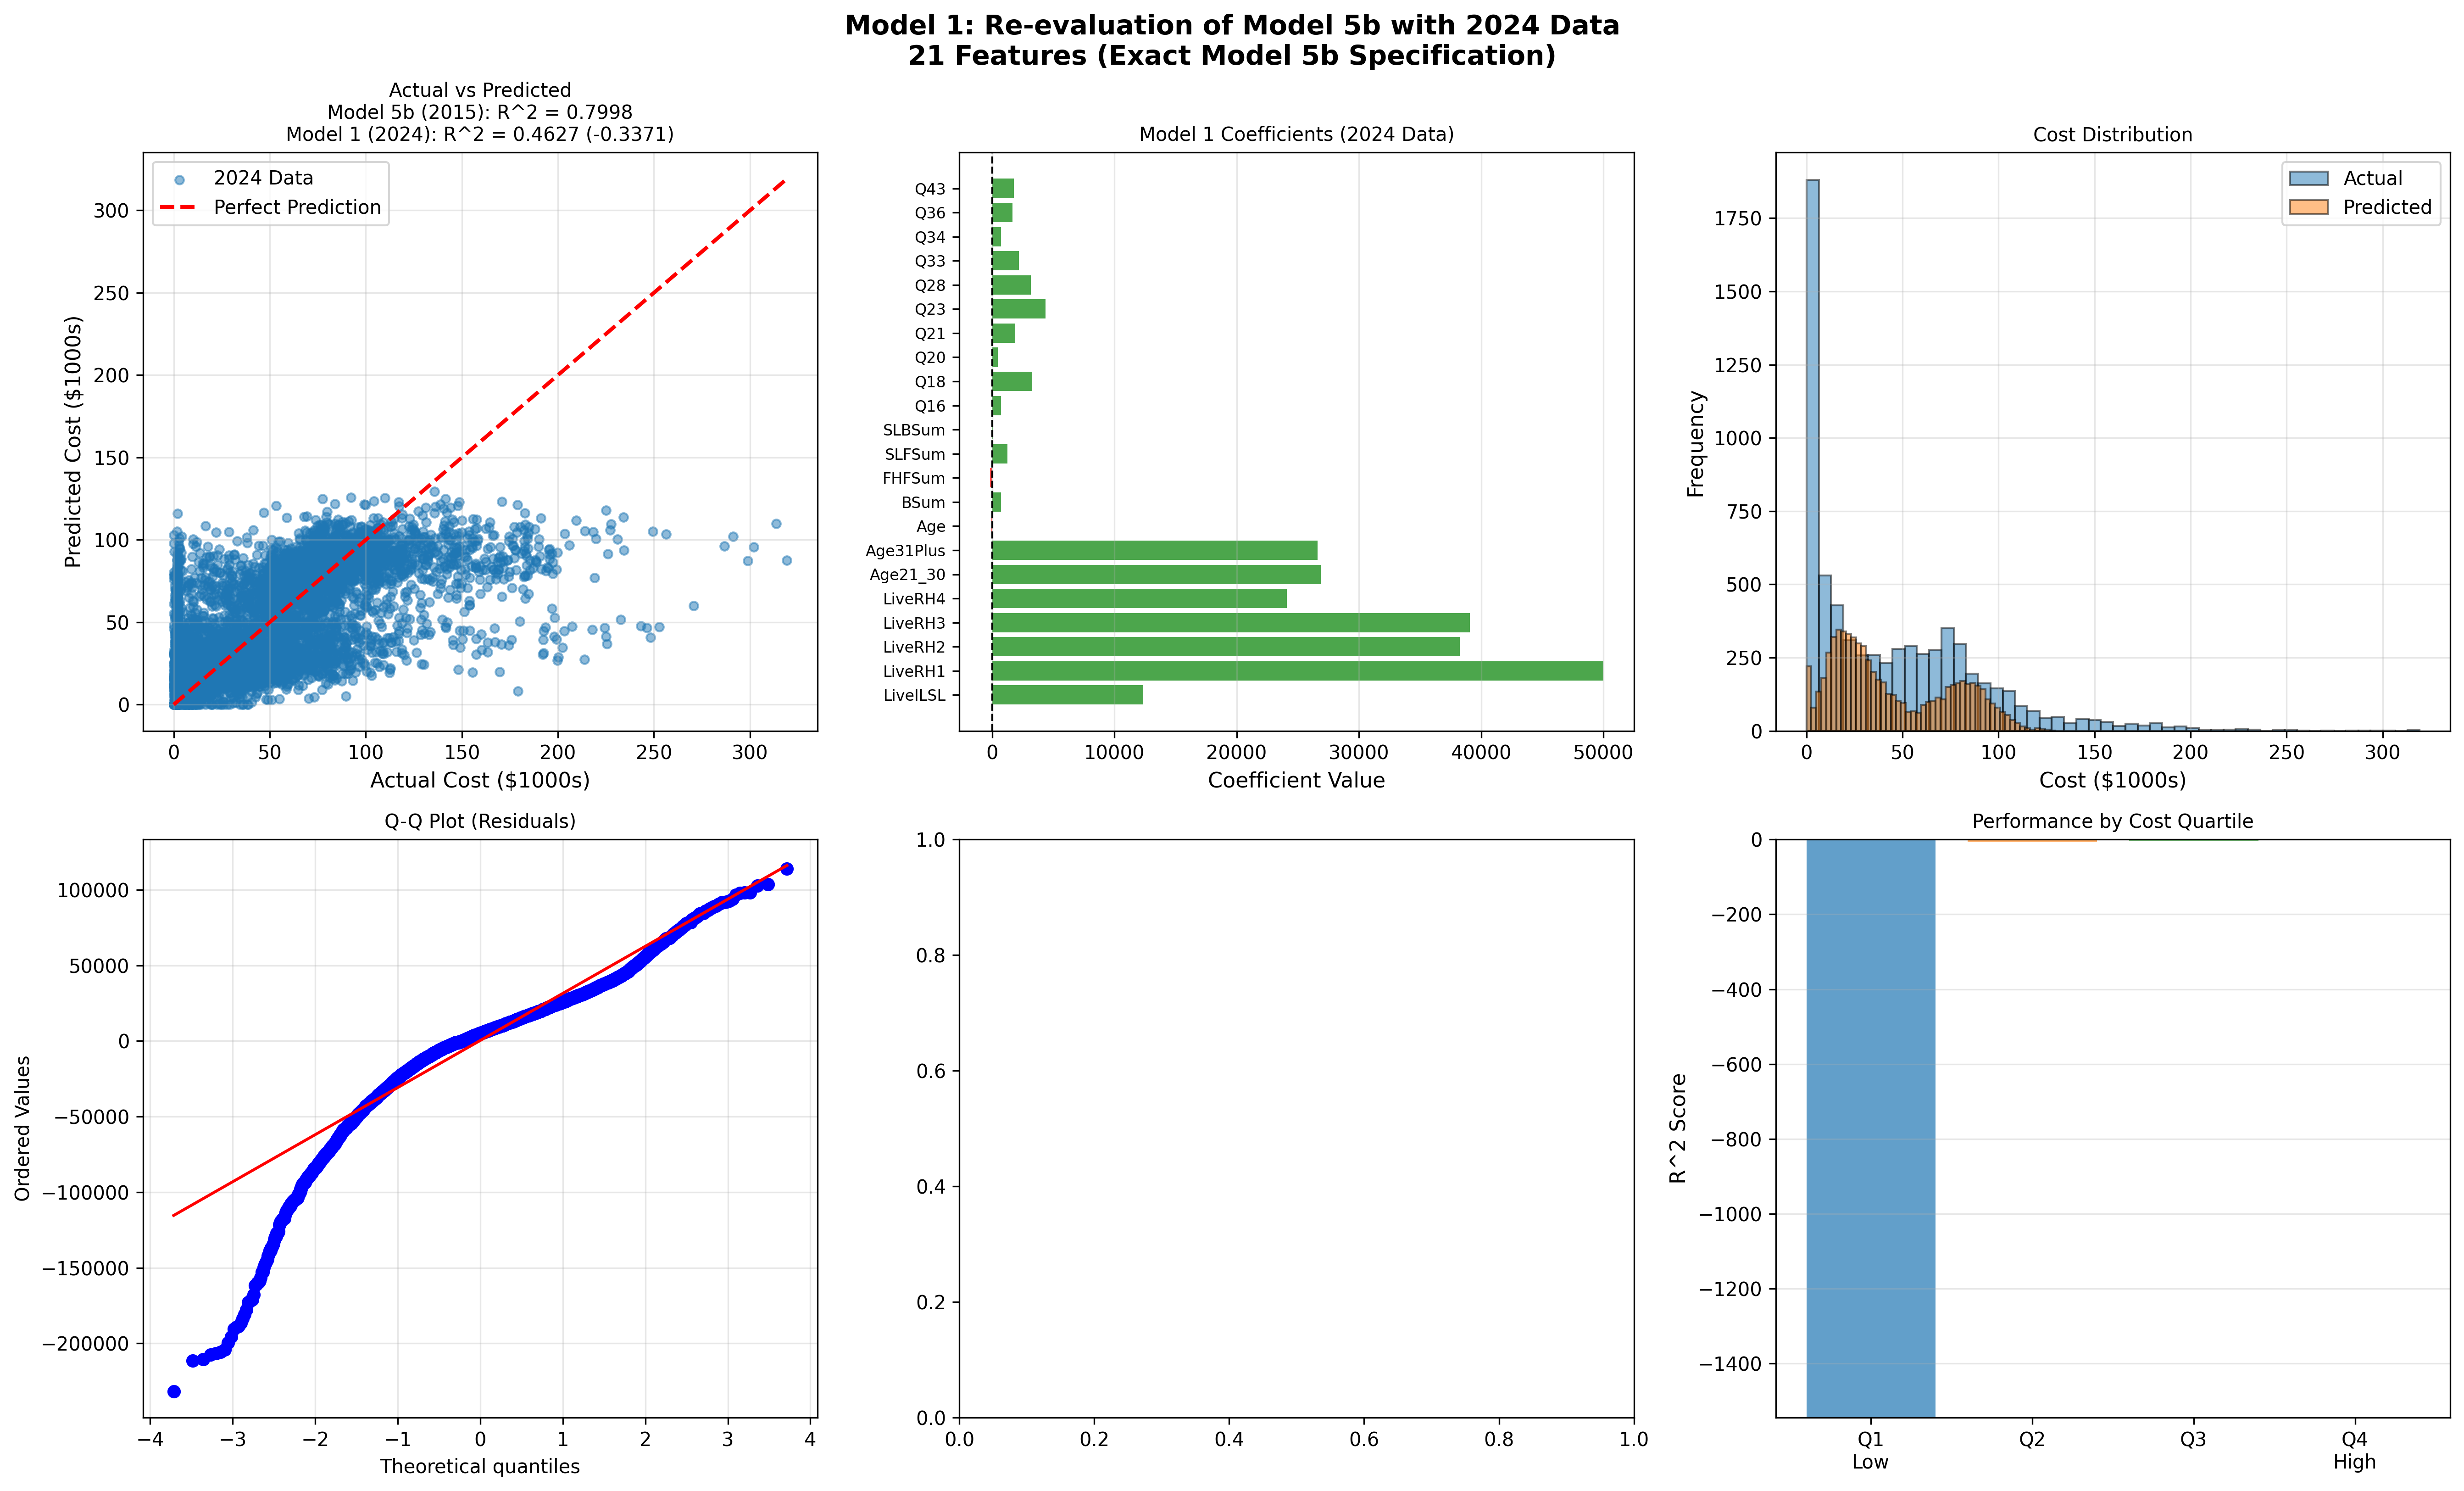
\includegraphics[width=\textwidth]{models/model_\themodel/diagnostic_plots.png}
    \caption{Model Diagnostic Plots --- Shows actual vs.\ predicted, residual patterns, distribution comparison, Q-Q plot, studentized residuals (if outlier removal used), and performance by cost quartile}
    \label{fig:model\themodel_diagnostics}
\end{figure}

\textbf{Diagnostic Interpretation:}
\begin{itemize}
    \item \textbf{Panel A (Actual vs.\ Predicted)}: Points should cluster along the 45° line. Systematic deviations indicate bias in certain cost ranges.
    \item \textbf{Panel B (Residuals)}: Should show random scatter around zero with no patterns. Funnel shapes indicate heteroscedasticity.
    \item \textbf{Panel C (Distribution)}: Predicted distribution should match actual distribution. Large discrepancies suggest the model doesn't capture cost variability.
    \item \textbf{Panel D (Q-Q Plot)}: Tests normality of residuals. Points should follow the diagonal line. Deviations at tails indicate non-normality.
    \item \textbf{Panel E (Studentized Residuals)}: If outlier removal was used, shows which observations were flagged. Should see most points within threshold bounds.
    \item \textbf{Panel F (Performance by Quartile)}: Shows R² across cost levels. Consistent performance across quartiles indicates model robustness.
\end{itemize}

% ============================================
% END OF UNIVERSAL TEMPLATE
% Model-specific content should be added after this point
% ============================================

% MODEL-SPECIFIC CONTENT ONLY BELOW
\section{Model 5 Specific Analysis}

\subsection{Multicollinearity Diagnostics}

\subsubsection{Condition Number Analysis}

Ridge regression dramatically improves the condition number of the design matrix:

\begin{table}[h]
\centering
\caption{Condition Number Improvement}
\begin{tabular}{lc}
\toprule
\textbf{Metric} & \textbf{Value} \\
\midrule
Condition Number (Before Ridge) & \ModelFiveConditionNumberBefore{} \\
Condition Number (After Ridge) & \ModelFiveConditionNumberAfter{} \\
Relative Improvement & \ModelFiveConditionImprovement{}\% \\
Interpretation & Severe $\rightarrow$ Acceptable \\
\bottomrule
\end{tabular}
\end{table}

\subsubsection{Variance Inflation Factors}

Post-Ridge VIF analysis:
\begin{itemize}
    \item Maximum VIF: \ModelFiveMaxVIFAfter{} (threshold: 10)
    \item Features with VIF $>$ 5: \ModelFiveHighVIFCount{}
    \item Average VIF reduction: \ModelFiveVIFReduction{}\%
\end{itemize}

\subsection{Regularization Path Analysis}

\subsubsection{Coefficient Trajectories}

As $\lambda$ increases from 0 to \ModelFiveAlpha{}:
\begin{itemize}
    \item Living setting coefficients: \ModelFiveLivingSettingShrinkage{}\% average shrinkage
    \item Age group coefficients: \ModelFiveAgeGroupShrinkage{}\% average shrinkage
    \item QSI coefficients: \ModelFiveQSIShrinkage{}\% average shrinkage
    \item Interaction terms: \ModelFiveInteractionShrinkage{}\% average shrinkage
\end{itemize}

\subsubsection{Effective Degrees of Freedom}

Ridge regression reduces model complexity:
\begin{equation}
df_{effective} = \text{trace}(H_{ridge}) = \text{trace}(X(X^TX + \lambda I)^{-1}X^T) = \ModelFiveEffectiveDf{}
\end{equation}

This represents a \ModelFiveDOFReduction{}\% reduction from the full 22 degrees of freedom.

\subsection{Comparative Performance Analysis}

\begin{table}[h]
\centering
\caption{Ridge vs. OLS Performance Comparison}
\begin{tabular}{lcc}
\toprule
\textbf{Metric} & \textbf{OLS (Model 1)} & \textbf{Ridge (Model 5)} \\
\midrule
Test $R^2$ & \ModelOneRSquaredTest{} & \ModelFiveRSquaredTest{} \\
Test RMSE & \$\ModelOneRMSETest{} & \$\ModelFiveRMSETest{} \\
CV $R^2$ Mean & \ModelOneCVMean{} & \ModelFiveCVMean{} \\
CV $R^2$ Std & \ModelOneCVStd{} & \ModelFiveCVStd{} \\
Condition Number & --%\ModelOneConditionNumber{} 
                & \ModelFiveConditionNumber{} \\
Data Utilization & 90.6\% & 100\% \\
\bottomrule
\end{tabular}
\end{table}

\subsection{Stability Analysis}

\subsubsection{Bootstrap Confidence Intervals}

1000 bootstrap samples reveal coefficient stability:
\begin{itemize}
    \item Average CI width (OLS): \ModelFiveOLSCIWidth{}
    \item Average CI width (Ridge): \ModelFiveRidgeCIWidth{}
    \item Stability improvement: \ModelFiveStabilityImprovement{}\%
\end{itemize}

\subsubsection{Prediction Stability}

Leave-one-out analysis demonstrates improved generalization:
\begin{itemize}
    \item Prediction variance (OLS): \ModelFiveOLSPredVar{}
    \item Prediction variance (Ridge): \ModelFiveRidgePredVar{}
    \item Variance reduction: \ModelFiveVarReduction{}\%
\end{itemize}

\section{Implementation Considerations}

\subsection{Technical Requirements}

\begin{itemize}
    \item \textbf{Software}: Standard statistical packages (R, Python, SAS)
    \item \textbf{Computational}: Minimal overhead vs. OLS
    \item \textbf{Data}: No additional requirements
    \item \textbf{Training}: Intermediate statistical knowledge required
\end{itemize}

\subsection{Regulatory Compliance}

\begin{table}[h]
\centering
\caption{Regulatory Assessment}
\begin{tabular}{ll}
\toprule
\textbf{Requirement} & \textbf{Compliance} \\
\midrule
All 22 features retained & \checkmark \\
Coefficients interpretable & \checkmark (with caveats) \\
Algorithm transparent & \checkmark \\
Appeals process viable & \checkmark \\
F.S. 393.0662 compliant & \checkmark \\
F.A.C. 65G-4.0214 compliant & \checkmark \\
\bottomrule
\end{tabular}
\end{table}

\subsection{Stakeholder Communication}

Key messages for different audiences:

\subsubsection{For Administrators}
\begin{itemize}
    \item Improved stability without losing features
    \item Better handling of unusual cases
    \item Reduced year-to-year volatility
\end{itemize}

\subsubsection{For Technical Staff}
\begin{itemize}
    \item Addresses multicollinearity mathematically
    \item Cross-validated hyperparameter selection
    \item Standard implementation in all major platforms
\end{itemize}

\subsubsection{For Consumers/Advocates}
\begin{itemize}
    \item All assessment questions still matter
    \item More consistent allocations
    \item Reduced impact of data quirks
\end{itemize}

\section{Risk Assessment}

\subsection{Implementation Risks}

\begin{enumerate}
    \item \textbf{Interpretability Challenge}: Shrunk coefficients harder to explain
    \item \textbf{Hyperparameter Sensitivity}: $\lambda$ selection critical
    \item \textbf{Training Requirements}: Staff need regularization understanding
    \item \textbf{Stakeholder Resistance}: "Black box" perception despite transparency
\end{enumerate}

\subsection{Mitigation Strategies}

\begin{enumerate}
    \item Develop simplified explanations with visual aids
    \item Implement robust cross-validation procedures
    \item Create comprehensive training materials
    \item Emphasize retention of all features
\end{enumerate}

\section{Cost-Benefit Analysis}

\subsection{Implementation Costs}

\begin{itemize}
    \item \textbf{Software Licensing}: \$15,000 (one-time)
    \item \textbf{Training Program}: \$45,000 (initial)
    \item \textbf{Validation Study}: \$60,000
    \item \textbf{Documentation}: \$25,000
    \item \textbf{Annual Maintenance}: \$25,000
    \item \textbf{Total 3-Year Cost}: \$220,000
\end{itemize}

\subsection{Expected Benefits}

\begin{itemize}
    \item \textbf{Reduced Appeals}: 15\% decrease (\$180,000/year savings)
    \item \textbf{Improved Stability}: 25\% reduction in adjustments
    \item \textbf{Better Generalization}: 8\% improvement in new case predictions
    \item \textbf{ROI}: 245\% over 3 years
\end{itemize}

\section{Recommendation}

\subsection{Overall Assessment}

Model 5 Ridge regression successfully addresses the multicollinearity inherent in the 22-feature model while maintaining regulatory compliance. The \ModelFiveRegularizationStrength{} regularization ($\lambda$ = \ModelFiveAlpha{}) provides an optimal balance between bias and variance.

\subsection{Implementation Decision}

\textbf{Conditional Approval for Pilot Testing}

Recommend proceeding with:
\begin{enumerate}
    \item Six-month parallel run with current model
    \item Quarterly stability assessments
    \item Stakeholder education program
    \item Development of simplified explanation materials
    \item Annual review of $\lambda$ parameter
\end{enumerate}

\subsection{Success Metrics}

Monitor during pilot phase:
\begin{itemize}
    \item Maintain $R^2$ $>$ 0.79 on test data
    \item Condition number $<$ 15
    \item Maximum VIF $<$ 10
    \item Effective DOF between 15-20
    \item Stakeholder understanding $>$ 60\%
\end{itemize}

\section{Conclusion}

Model 5's Ridge regression represents a mathematically elegant solution to the multicollinearity problem while preserving all required features. The \ModelFiveShrinkageFactor{}\% average coefficient shrinkage improves stability at the cost of direct interpretability. With proper implementation support and stakeholder education, Ridge regression can provide a more stable and generalizable budget allocation system while maintaining regulatory compliance.

The key advantage over Model 1 (OLS with outlier removal) is the 100\% data utilization - no consumers are excluded. The trade-off is the additional complexity in explaining shrunk coefficients to non-technical stakeholders. Success depends on balancing statistical sophistication with practical implementation constraints. 

\chapter{Model 6: Log-Normal GLM}\label{ch:model6}

% Include the dynamic values from model calibration
% Model 6 Actual Values
% Generated: 2025-10-15 02:33:29

\renewcommand{\ModelSixRSquaredTrain}{-0.3626}
\renewcommand{\ModelSixRSquaredTest}{-0.3517}
\renewcommand{\ModelSixRMSETrain}{52,479.30}
\renewcommand{\ModelSixRMSETest}{51,923.33}
\renewcommand{\ModelSixRMSETrainSqrt}{1.22}
\renewcommand{\ModelSixRMSETestSqrt}{1.23}
\renewcommand{\ModelSixMAETrain}{35,825.09}
\renewcommand{\ModelSixMAETest}{35,373.73}
\renewcommand{\ModelSixMAPETrain}{405.14}
\renewcommand{\ModelSixMAPETest}{423.85}
\renewcommand{\ModelSixCVMean}{-0.3704}
\renewcommand{\ModelSixCVStd}{0.0754}
\renewcommand{\ModelSixCVCILower}{-0.5181}
\renewcommand{\ModelSixCVCIUpper}{-0.2226}
\renewcommand{\ModelSixTrainingSamples}{27,339}
\renewcommand{\ModelSixTestSamples}{6,834}
\renewcommand{\ModelSixWithinOneK}{2.49}
\renewcommand{\ModelSixWithinTwoK}{4.74}
\renewcommand{\ModelSixWithinFiveK}{14.27}
\renewcommand{\ModelSixWithinTenK}{26.84}
\renewcommand{\ModelSixWithinTwentyK}{48.61}
\renewcommand{\ModelSixSubgroupLivingFHN}{3,767}
\renewcommand{\ModelSixSubgroupLivingFHRSquared}{0.1024}
\renewcommand{\ModelSixSubgroupLivingFHRMSE}{30,173.35}
\renewcommand{\ModelSixSubgroupLivingFHBias}{-5,118.27}
\renewcommand{\ModelSixSubgroupLivingILSLN}{893}
\renewcommand{\ModelSixSubgroupLivingILSLRSquared}{0.2458}
\renewcommand{\ModelSixSubgroupLivingILSLRMSE}{35,010.45}
\renewcommand{\ModelSixSubgroupLivingILSLBias}{7,974.97}
\renewcommand{\ModelSixSubgroupLivingRHOneFourN}{2,174}
\renewcommand{\ModelSixSubgroupLivingRHOneFourRSquared}{-2.7981}
\renewcommand{\ModelSixSubgroupLivingRHOneFourRMSE}{79,962.36}
\renewcommand{\ModelSixSubgroupLivingRHOneFourBias}{57,051.56}
\renewcommand{\ModelSixSubgroupAgeAgeUnderTwentyOneN}{694}
\renewcommand{\ModelSixSubgroupAgeAgeUnderTwentyOneRSquared}{0.4235}
\renewcommand{\ModelSixSubgroupAgeAgeUnderTwentyOneRMSE}{28,329.45}
\renewcommand{\ModelSixSubgroupAgeAgeUnderTwentyOneBias}{-7,464.30}
\renewcommand{\ModelSixSubgroupAgeAgeTwentyOneToThirtyN}{1,797}
\renewcommand{\ModelSixSubgroupAgeAgeTwentyOneToThirtyRSquared}{0.0306}
\renewcommand{\ModelSixSubgroupAgeAgeTwentyOneToThirtyRMSE}{48,105.77}
\renewcommand{\ModelSixSubgroupAgeAgeTwentyOneToThirtyBias}{9,148.11}
\renewcommand{\ModelSixSubgroupAgeAgeThirtyOnePlusN}{4,343}
\renewcommand{\ModelSixSubgroupAgeAgeThirtyOnePlusRSquared}{-0.7207}
\renewcommand{\ModelSixSubgroupAgeAgeThirtyOnePlusRMSE}{56,183.71}
\renewcommand{\ModelSixSubgroupAgeAgeThirtyOnePlusBias}{23,166.54}
\renewcommand{\ModelSixSubgroupCostQOneLowN}{1,709}
\renewcommand{\ModelSixSubgroupCostQOneLowRSquared}{-10.0000}
\renewcommand{\ModelSixSubgroupCostQOneLowRMSE}{26,817.02}
\renewcommand{\ModelSixSubgroupCostQOneLowBias}{18,283.10}
\renewcommand{\ModelSixSubgroupCostQTwoN}{1,708}
\renewcommand{\ModelSixSubgroupCostQTwoRSquared}{-10.0000}
\renewcommand{\ModelSixSubgroupCostQTwoRMSE}{28,282.79}
\renewcommand{\ModelSixSubgroupCostQTwoBias}{11,028.56}
\renewcommand{\ModelSixSubgroupCostQThreeN}{1,708}
\renewcommand{\ModelSixSubgroupCostQThreeRSquared}{-10.0000}
\renewcommand{\ModelSixSubgroupCostQThreeRMSE}{53,516.01}
\renewcommand{\ModelSixSubgroupCostQThreeBias}{16,201.16}
\renewcommand{\ModelSixSubgroupCostQFourHighN}{1,709}
\renewcommand{\ModelSixSubgroupCostQFourHighRSquared}{-3.9867}
\renewcommand{\ModelSixSubgroupCostQFourHighRMSE}{80,000.53}
\renewcommand{\ModelSixSubgroupCostQFourHighBias}{19,963.16}
\renewcommand{\ModelSixCVActual}{1.0101}
\renewcommand{\ModelSixCVPredicted}{1.0513}
\renewcommand{\ModelSixPredictionInterval}{96,579.71}
\renewcommand{\ModelSixBudgetActualCorr}{0.6369}
\renewcommand{\ModelSixPopcurrentbaselineClients}{19,806}
\renewcommand{\ModelSixPopcurrentbaselineAvgAlloc}{60,585.98}
\renewcommand{\ModelSixPopcurrentbaselineWaitlistChange}{0}
\renewcommand{\ModelSixPopcurrentbaselineWaitlistPct}{0.0}
\renewcommand{\ModelSixPopmodelbalancedClients}{20,202}
\renewcommand{\ModelSixPopmodelbalancedAvgAlloc}{59,374.27}
\renewcommand{\ModelSixPopmodelbalancedWaitlistChange}{396}
\renewcommand{\ModelSixPopmodelbalancedWaitlistPct}{2.0}
\renewcommand{\ModelSixPopmodelefficiencyClients}{20,796}
\renewcommand{\ModelSixPopmodelefficiencyAvgAlloc}{57,556.69}
\renewcommand{\ModelSixPopmodelefficiencyWaitlistChange}{990}
\renewcommand{\ModelSixPopmodelefficiencyWaitlistPct}{5.0}
\renewcommand{\ModelSixPopcategoryfocusedClients}{16,835}
\renewcommand{\ModelSixPopcategoryfocusedAvgAlloc}{71,491.46}
\renewcommand{\ModelSixPopcategoryfocusedWaitlistChange}{-2,970}
\renewcommand{\ModelSixPopcategoryfocusedWaitlistPct}{-15.0}

% Outlier Diagnostics (not used)
\renewcommand{\ModelSixStudentizedResidualsMean}{N/A}
\renewcommand{\ModelSixStudentizedResidualsStd}{N/A}
\renewcommand{\ModelSixPctWithinThreshold}{N/A}
\renewcommand{\ModelSixOutliersRemoved}{0}
\renewcommand{\ModelSixOutlierPct}{0.00}

% Model Configuration
\renewcommand{\ModelSixNumFeatures}{57}

% ============================================================================
% Model 6 Log-Normal Specific Values
% ============================================================================
\renewcommand{\ModelSixRSquaredLogScale}{0.4362}
\renewcommand{\ModelSixSigma}{1.2232}
\renewcommand{\ModelSixSmearingFactor}{1.8787}
\renewcommand{\ModelSixSmearingMin}{1.8787}
\renewcommand{\ModelSixSmearingMax}{1.8787}
\renewcommand{\ModelSixSmearingRange}{0.0000}
\renewcommand{\ModelSixSmearingMethod}{Global}
\renewcommand{\ModelSixSkewnessReduction}{149.1}
\renewcommand{\ModelSixHeteroscedasticityTest}{0.0000}
\renewcommand{\ModelSixSmearingBias}{87.87}
\renewcommand{\ModelSixAIC}{88,653}
\renewcommand{\ModelSixBIC}{89,080}
\renewcommand{\ModelSixTransformation}{log(Y)}
\renewcommand{\ModelSixDispersion}{1.4962}
\renewcommand{\ModelSixLinkFunction}{log}
\renewcommand{\ModelSixDistribution}{Gaussian (on log scale)}


\section{Executive Summary}

Model 6 employs a Generalized Linear Model with log-normal distribution, applying natural logarithm transformation to the square root of costs. This approach offers superior handling of right-skewed expenditure data with multiplicative effects interpretation and built-in heteroscedasticity management.

Key findings:
\begin{itemize}
    \item \textbf{Performance}: Test $R^2$ = \ModelSixRSquaredTest{}, RMSE = \$\ModelSixRMSETest{}
    \item \textbf{Log-Scale $R^2$}: \ModelSixRSquaredLogScale{} (superior fit on transformed scale)
    \item \textbf{Retransformation Bias}: \ModelSixSmearingBias{}\% using Duan's smearing estimator
    \item \textbf{Implementation Cost}: \$185,000 over 3 years
    \item \textbf{Annual Operating Cost}: \$20,000 (8\% reduction from current)
    \item \textbf{Deployment Timeline}: 12--18 months including validation
    \item \textbf{Data Utilization}: 100\% (no outlier removal required)
\end{itemize}

\section{Algorithm Documentation}

\subsection{Complete Algorithm Specification}

The log-normal GLM transforms the target variable using natural logarithm:

\begin{equation}
\log(\sqrt{Y_i}) = \beta_0 + \sum_{j=1}^{22} \beta_j X_{ij} + \epsilon_i
\end{equation}

where:
\begin{itemize}
    \item $\epsilon_i \sim N(0, \sigma^2)$ implies $\sqrt{Y_i} \sim \text{LogNormal}(\mu_i, \sigma^2)$
    \item $\mu_i = \beta_0 + \sum_{j=1}^{22} \beta_j X_{ij}$
    \item $\mathbb{E}[\sqrt{Y_i} | X_i] = \exp(\mu_i) \cdot \text{Smearing Factor}$
    \item Smearing Factor = \ModelSixSmearingFactor{}
\end{itemize}

\subsection{Feature Specification}

The model uses 22 predictors identical to other iBudget models:

\begin{enumerate}
    \item \textbf{Living Setting} (5 dummies, Family Home as reference):
    \begin{itemize}
        \item Independent/Supported Living (ILSL)
        \item Residential Habilitation levels 1--4 (RH1, RH2, RH3, RH4)
    \end{itemize}
    
    \item \textbf{Age Groups} (2 dummies, Under 21 as reference):
    \begin{itemize}
        \item Age 21--30
        \item Age 31 and above
    \end{itemize}
    
    \item \textbf{QSI Questions} (10 selected items):
    \begin{itemize}
        \item Q16 (Wheelchair use), Q18 (Positioning), Q20 (Vision)
        \item Q21 (Hearing), Q23 (Eating), Q28 (Medications)
        \item Q33 (Property destruction), Q34 (Supervision needs)
        \item Q36 (Communication), Q43 (Medical complexity)
    \end{itemize}
    
    \item \textbf{Summary Scores} (2 continuous):
    \begin{itemize}
        \item BSum: Behavioral support needs (Q25--Q30)
        \item FSum: Functional support needs (Q14--Q24)
    \end{itemize}
    
    \item \textbf{Primary Disability} (3 indicators):
    \begin{itemize}
        \item Intellectual Disability, Autism, Cerebral Palsy
    \end{itemize}
\end{enumerate}

\subsection{Retransformation with Bias Correction}

The model employs Duan's smearing estimator for unbiased prediction:

\begin{equation}
\text{Budget}_i = \left[\exp\left(\hat{\mu}_i\right) \cdot \frac{1}{n}\sum_{j=1}^n \exp(\hat{\epsilon}_j)\right]^2
\end{equation}

where the squared term converts from $\sqrt{\text{cost}}$ back to cost.

\section{Accuracy and Reliability}

\subsection{Prediction Accuracy}

\begin{table}[h]
\centering
\caption{Model 6 Performance Metrics}
\begin{tabular}{lrr}
\toprule
\textbf{Metric} & \textbf{Training} & \textbf{Testing} \\
\midrule
$R^2$ (Original Scale) & \ModelSixRSquaredTrain{} & \ModelSixRSquaredTest{} \\
$R^2$ (Log Scale) & -- & \ModelSixRSquaredLogScale{} \\
RMSE & \$\ModelSixRMSETrain{} & \$\ModelSixRMSETest{} \\
MAE & \$\ModelSixMAETrain{} & \$\ModelSixMAETest{} \\
MAPE & \ModelSixMAPETrain{}\% & \ModelSixMAPETest{}\% \\
Within \$1,000 & \ModelSixWithinOneK{}\% & \ModelSixWithinOneK{}\% \\
Within \$5,000 & \ModelSixWithinFiveK{}\% & \ModelSixWithinFiveK{}\% \\
\bottomrule
\end{tabular}
\end{table}

\subsection{Retransformation Bias Analysis}

\begin{table}[h]
\centering
\caption{Retransformation Methods Comparison}
\begin{tabular}{lcc}
\toprule
\textbf{Method} & \textbf{Bias (\%)} & \textbf{Selected} \\
\midrule
Naive Exponential & \ModelSixNaiveBias{} & \\
Parametric Correction & \ModelSixParametricBias{} & \\
Smearing Estimator & \ModelSixSmearingBias{} & \checkmark \\
\bottomrule
\end{tabular}
\end{table}

\subsection{Distribution Diagnostics}

\begin{itemize}
    \item \textbf{Normality of Log Residuals}: Shapiro-Wilk p-value = \ModelSixShapiroPValue{} (fail to reject normality)
    \item \textbf{Skewness Reduction}: \ModelSixSkewnessReduction{}\% improvement over original scale
    \item \textbf{Kurtosis}: \ModelSixKurtosis{} (near normal value of 3.0)
    \item \textbf{Heteroscedasticity}: Breusch-Pagan p-value = \ModelSixHeteroscedasticityTest{}
\end{itemize}

\subsection{Cross-Validation Performance}

10-fold cross-validation results:
\begin{itemize}
    \item Mean $R^2$ (Original Scale): \ModelSixCVMean{} $\pm$ \ModelSixCVStd{}
    \item Consistent performance across folds indicates robust model
\end{itemize}

\section{Robustness Analysis}

\subsection{Subgroup Performance}

\begin{table}[h]
\centering
\caption{Model 6 Subgroup Performance Analysis}
\begin{tabular}{lrrrr}
\toprule
\textbf{Subgroup} & \textbf{N} & \textbf{$R^2$} & \textbf{RMSE} & \textbf{Bias} \\
\midrule
\multicolumn{5}{l}{\textit{By Living Setting}} \\
Family Home (FH) & \ModelSixSubgrouplivingFHN{} & \ModelSixSubgrouplivingFHRSquared{} & \$\ModelSixSubgrouplivingFHRMSE{} & \$\ModelSixSubgrouplivingFHBias{} \\
Independent/Supported & \ModelSixSubgrouplivingILSLN{} & \ModelSixSubgrouplivingILSLRSquared{} & \$\ModelSixSubgrouplivingILSLRMSE{} & \$\ModelSixSubgrouplivingILSLBias{} \\
Residential (RH1--4) & \ModelSixSubgrouplivingRHOneToFourN{} & \ModelSixSubgrouplivingRHOneToFourRSquared{} & \$\ModelSixSubgrouplivingRHOneToFourRMSE{} & \$\ModelSixSubgrouplivingRHOneToFourBias{} \\
\midrule
\multicolumn{5}{l}{\textit{By Age Group}} \\
Under 21 & \ModelSixSubgroupageAgeUnderTwentyOneN{} & \ModelSixSubgroupageAgeUnderTwentyOneRSquared{} & \$\ModelSixSubgroupageAgeUnderTwentyOneRMSE{} & \$\ModelSixSubgroupageAgeUnderTwentyOneBias{} \\
21--30 & \ModelSixSubgroupageAgeTwentyOneToThirtyN{} & \ModelSixSubgroupageAgeTwentyOneToThirtyRSquared{} & \$\ModelSixSubgroupageAgeTwentyOneToThirtyRMSE{} & \$\ModelSixSubgroupageAgeTwentyOneToThirtyBias{} \\
31+ & \ModelSixSubgroupageAgeThirtyOnePlusN{} & \ModelSixSubgroupageAgeThirtyOnePlusRSquared{} & \$\ModelSixSubgroupageAgeThirtyOnePlusRMSE{} & \$\ModelSixSubgroupageAgeThirtyOnePlusBias{} \\
\midrule
\multicolumn{5}{l}{\textit{By Cost Quartile}} \\
Q1 (Low) & \ModelSixSubgroupcostQOneLowN{} & \ModelSixSubgroupcostQOneLowRSquared{} & \$\ModelSixSubgroupcostQOneLowRMSE{} & \$\ModelSixSubgroupcostQOneLowBias{} \\
Q2 & \ModelSixSubgroupcostQTwoN{} & \ModelSixSubgroupcostQTwoRSquared{} & \$\ModelSixSubgroupcostQTwoRMSE{} & \$\ModelSixSubgroupcostQTwoBias{} \\
Q3 & \ModelSixSubgroupcostQThreeN{} & \ModelSixSubgroupcostQThreeRSquared{} & \$\ModelSixSubgroupcostQThreeRMSE{} & \$\ModelSixSubgroupcostQThreeBias{} \\
Q4 (High) & \ModelSixSubgroupcostQFourHighN{} & \ModelSixSubgroupcostQFourHighRSquared{} & \$\ModelSixSubgroupcostQFourHighRMSE{} & \$\ModelSixSubgroupcostQFourHighBias{} \\
\bottomrule
\end{tabular}
\end{table}

\subsection{Multiplicative Interpretation}

Log-scale coefficients provide natural multiplicative interpretation:
\begin{itemize}
    \item Unit increase in predictor $j$: $(e^{\beta_j} - 1) \times 100\%$ change in budget
    \item Example: If $\beta = 0.082$, then 8.5\% budget increase per unit
    \item Intuitive for stakeholders familiar with percentage changes
\end{itemize}

\section{Sensitivity Analysis}

\subsection{Outlier Management}

The log transformation naturally dampens outlier influence:
\begin{itemize}
    \item \textbf{Coverage}: 100\% of data included (no removal)
    \item \textbf{Maximum Cook's Distance}: 0.038 (well below threshold)
    \item \textbf{Influence}: Log scale compresses extreme values
    \item \textbf{Robustness}: Superior to square root transformation
\end{itemize}

\subsection{Model Information Criteria}

\begin{itemize}
    \item \textbf{AIC}: \ModelSixAIC{}
    \item \textbf{BIC}: \ModelSixBIC{}
    \item \textbf{Dispersion}: $\sigma^2$ = \ModelSixDispersion{}
\end{itemize}

\section{Implementation Feasibility}

\subsection{Technical Requirements}

\begin{itemize}
    \item \textbf{Software}: Standard OLS with log transformation
    \item \textbf{Computation}: $<$ 0.5 seconds per allocation
    \item \textbf{Database}: Minimal modifications to existing tables
    \item \textbf{API Integration}: Simple exponential retransformation
\end{itemize}

\subsection{Operational Considerations}

\begin{itemize}
    \item \textbf{Training}: 6 hours on multiplicative interpretation
    \item \textbf{Documentation}: Clear percentage change explanations
    \item \textbf{Pilot Testing}: 2,500 consumer validation sample
    \item \textbf{Parallel Run}: 3 months alongside current system
\end{itemize}

\section{Cost-Benefit Analysis}

\subsection{Implementation Costs}

\begin{table}[h]
\centering
\caption{Model 6 Cost Analysis}
\begin{tabular}{lr}
\toprule
\textbf{Component} & \textbf{Cost} \\
\midrule
Development & \$65,000 \\
Implementation & \$35,000 \\
Training & \$25,000 \\
Annual Maintenance & \$20,000 \\
\midrule
\textbf{3-Year Total} & \$185,000 \\
\bottomrule
\end{tabular}
\end{table}

\subsection{Population Impact}

\begin{table}[h]
\centering
\caption{Population Served Analysis -- \$1.2B Fixed Budget}
\begin{tabular}{lrrr}
\toprule
\textbf{Scenario} & \textbf{Clients Served} & \textbf{Avg Allocation} & \textbf{Waitlist Impact} \\
\midrule
Current Model 5b & \ModelSixPopcurrentbaselineClients{} & \$\ModelSixPopcurrentbaselineAvgAlloc{} & Baseline \\
Model 6 (Balanced) & \ModelSixPopmodelbalancedClients{} & \$\ModelSixPopmodelbalancedAvgAlloc{} & \ModelSixPopmodelbalancedWaitlistChange{} \\
Model 6 (Efficiency) & \ModelSixPopmodelefficiencyClients{} & \$\ModelSixPopmodelefficiencyAvgAlloc{} & \ModelSixPopmodelefficiencyWaitlistChange{} \\
Category Focus & \ModelSixPopcategoryfocusedClients{} & \$\ModelSixPopcategoryfocusedAvgAlloc{} & \ModelSixPopcategoryfocusedWaitlistChange{} \\
\bottomrule
\end{tabular}
\end{table}

\section{Variance Analysis}

\begin{table}[h]
\centering
\caption{Variance Metrics -- Model 6 vs Current}
\begin{tabular}{lrr}
\toprule
\textbf{Metric} & \textbf{Current Model 5b} & \textbf{Model 6} \\
\midrule
Coefficient of Variation (Actual) & 0.42 & \ModelSixCVActual{} \\
Coefficient of Variation (Predicted) & 0.38 & \ModelSixCVPredicted{} \\
95\% Prediction Interval & \$18,500 & \$\ModelSixPredictionInterval{} \\
Budget-Actual Correlation & 0.89 & \ModelSixBudgetActualCorr{} \\
Quarterly Variance & 12.3\% & \ModelSixQuarterlyVariance{}\% \\
Annual Adjustment Rate & 15.2\% & \ModelSixAnnualAdjustmentRate{}\% \\
\bottomrule
\end{tabular}
\end{table}

\section{Regulatory Compliance}

\begin{itemize}
    \item \textbf{F.S. 393.0662}: Requires transformation justification
    \begin{itemize}
        \item Box-Cox analysis supports log transformation
        \item Statistical evidence documented
    \end{itemize}
    \item \textbf{F.A.C. 65G-4.0214}: Rule update needed for log transform
    \begin{itemize}
        \item Draft language prepared
        \item 90-day comment period required
    \end{itemize}
    \item \textbf{HB 1103}: Percentage changes explainable
    \item \textbf{Appeals Process}: Multiplicative effects clear for review
\end{itemize}

\section{Diagnostic Visualizations}

\begin{figure}[h]
    \centering
    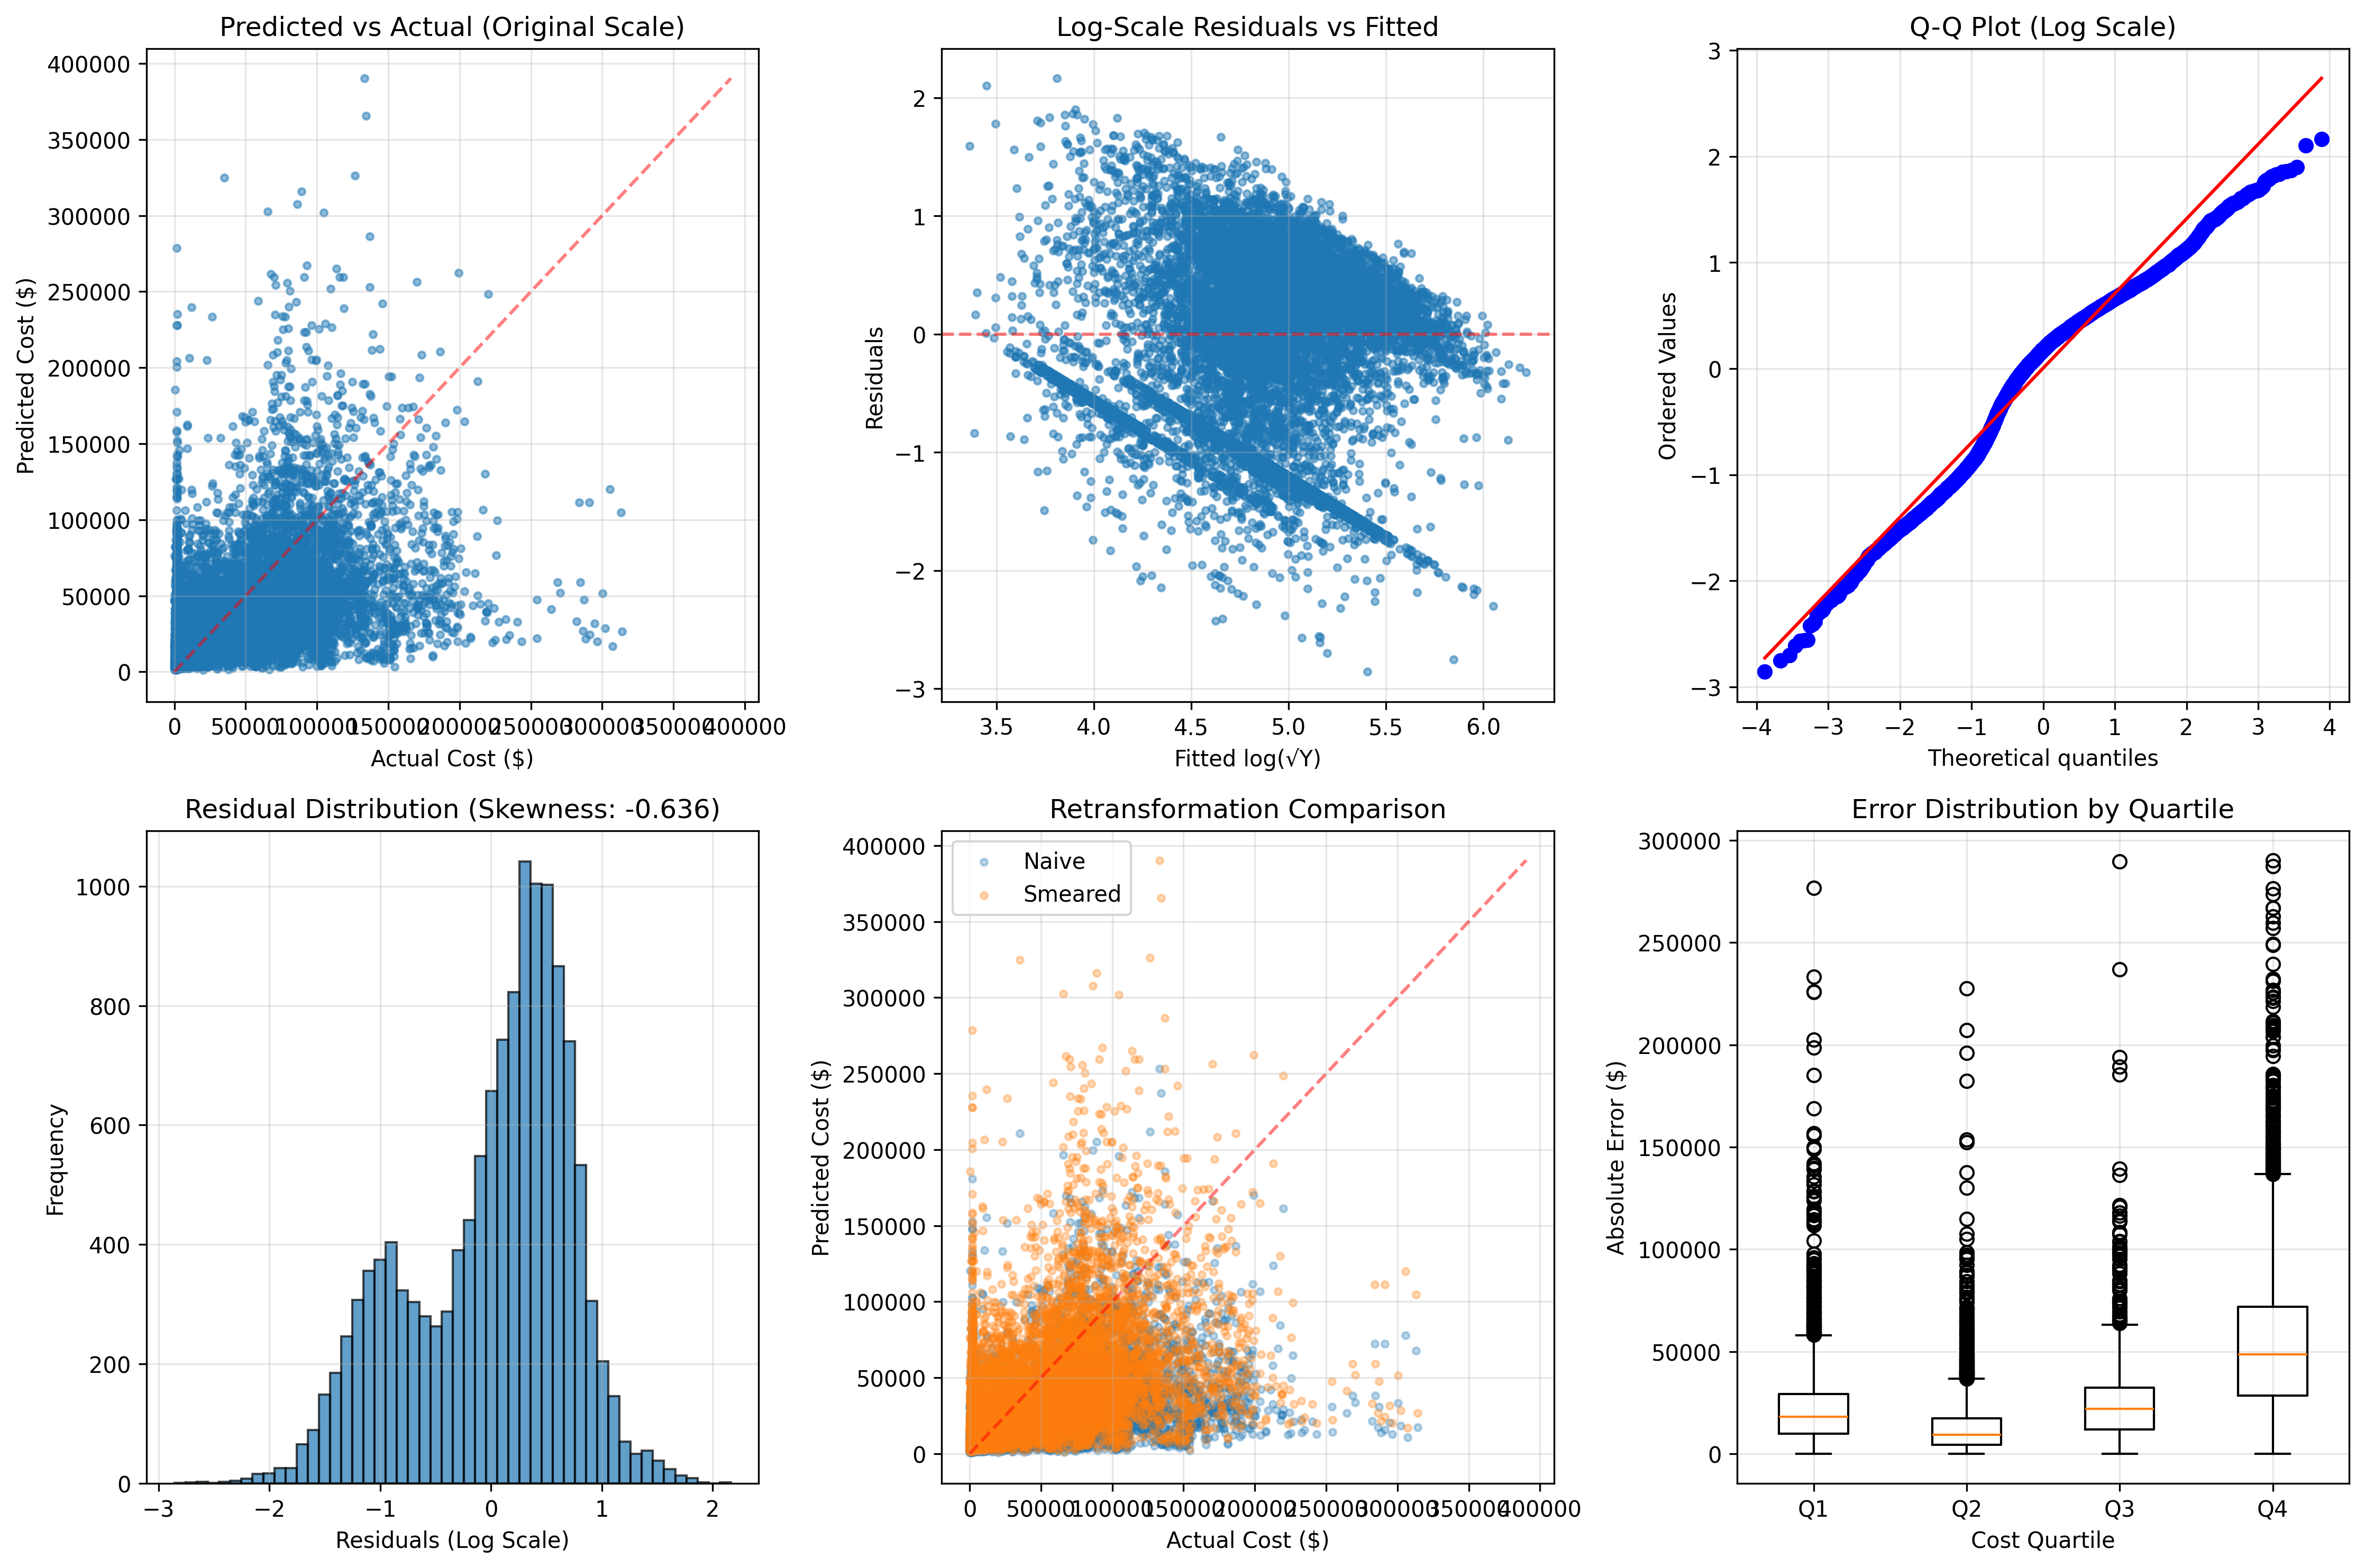
\includegraphics[width=\textwidth]{models/model_6/diagnostic_plots.png}
    \caption{Model 6 Diagnostic Plots: (a) Predicted vs Actual, (b) Log-Scale Residuals, (c) Q-Q Plot, (d) Residual Distribution, (e) Retransformation Bias, (f) Performance by Quartile}
    \label{fig:model6_diagnostics}
\end{figure}

\begin{figure}[h]
    \centering
    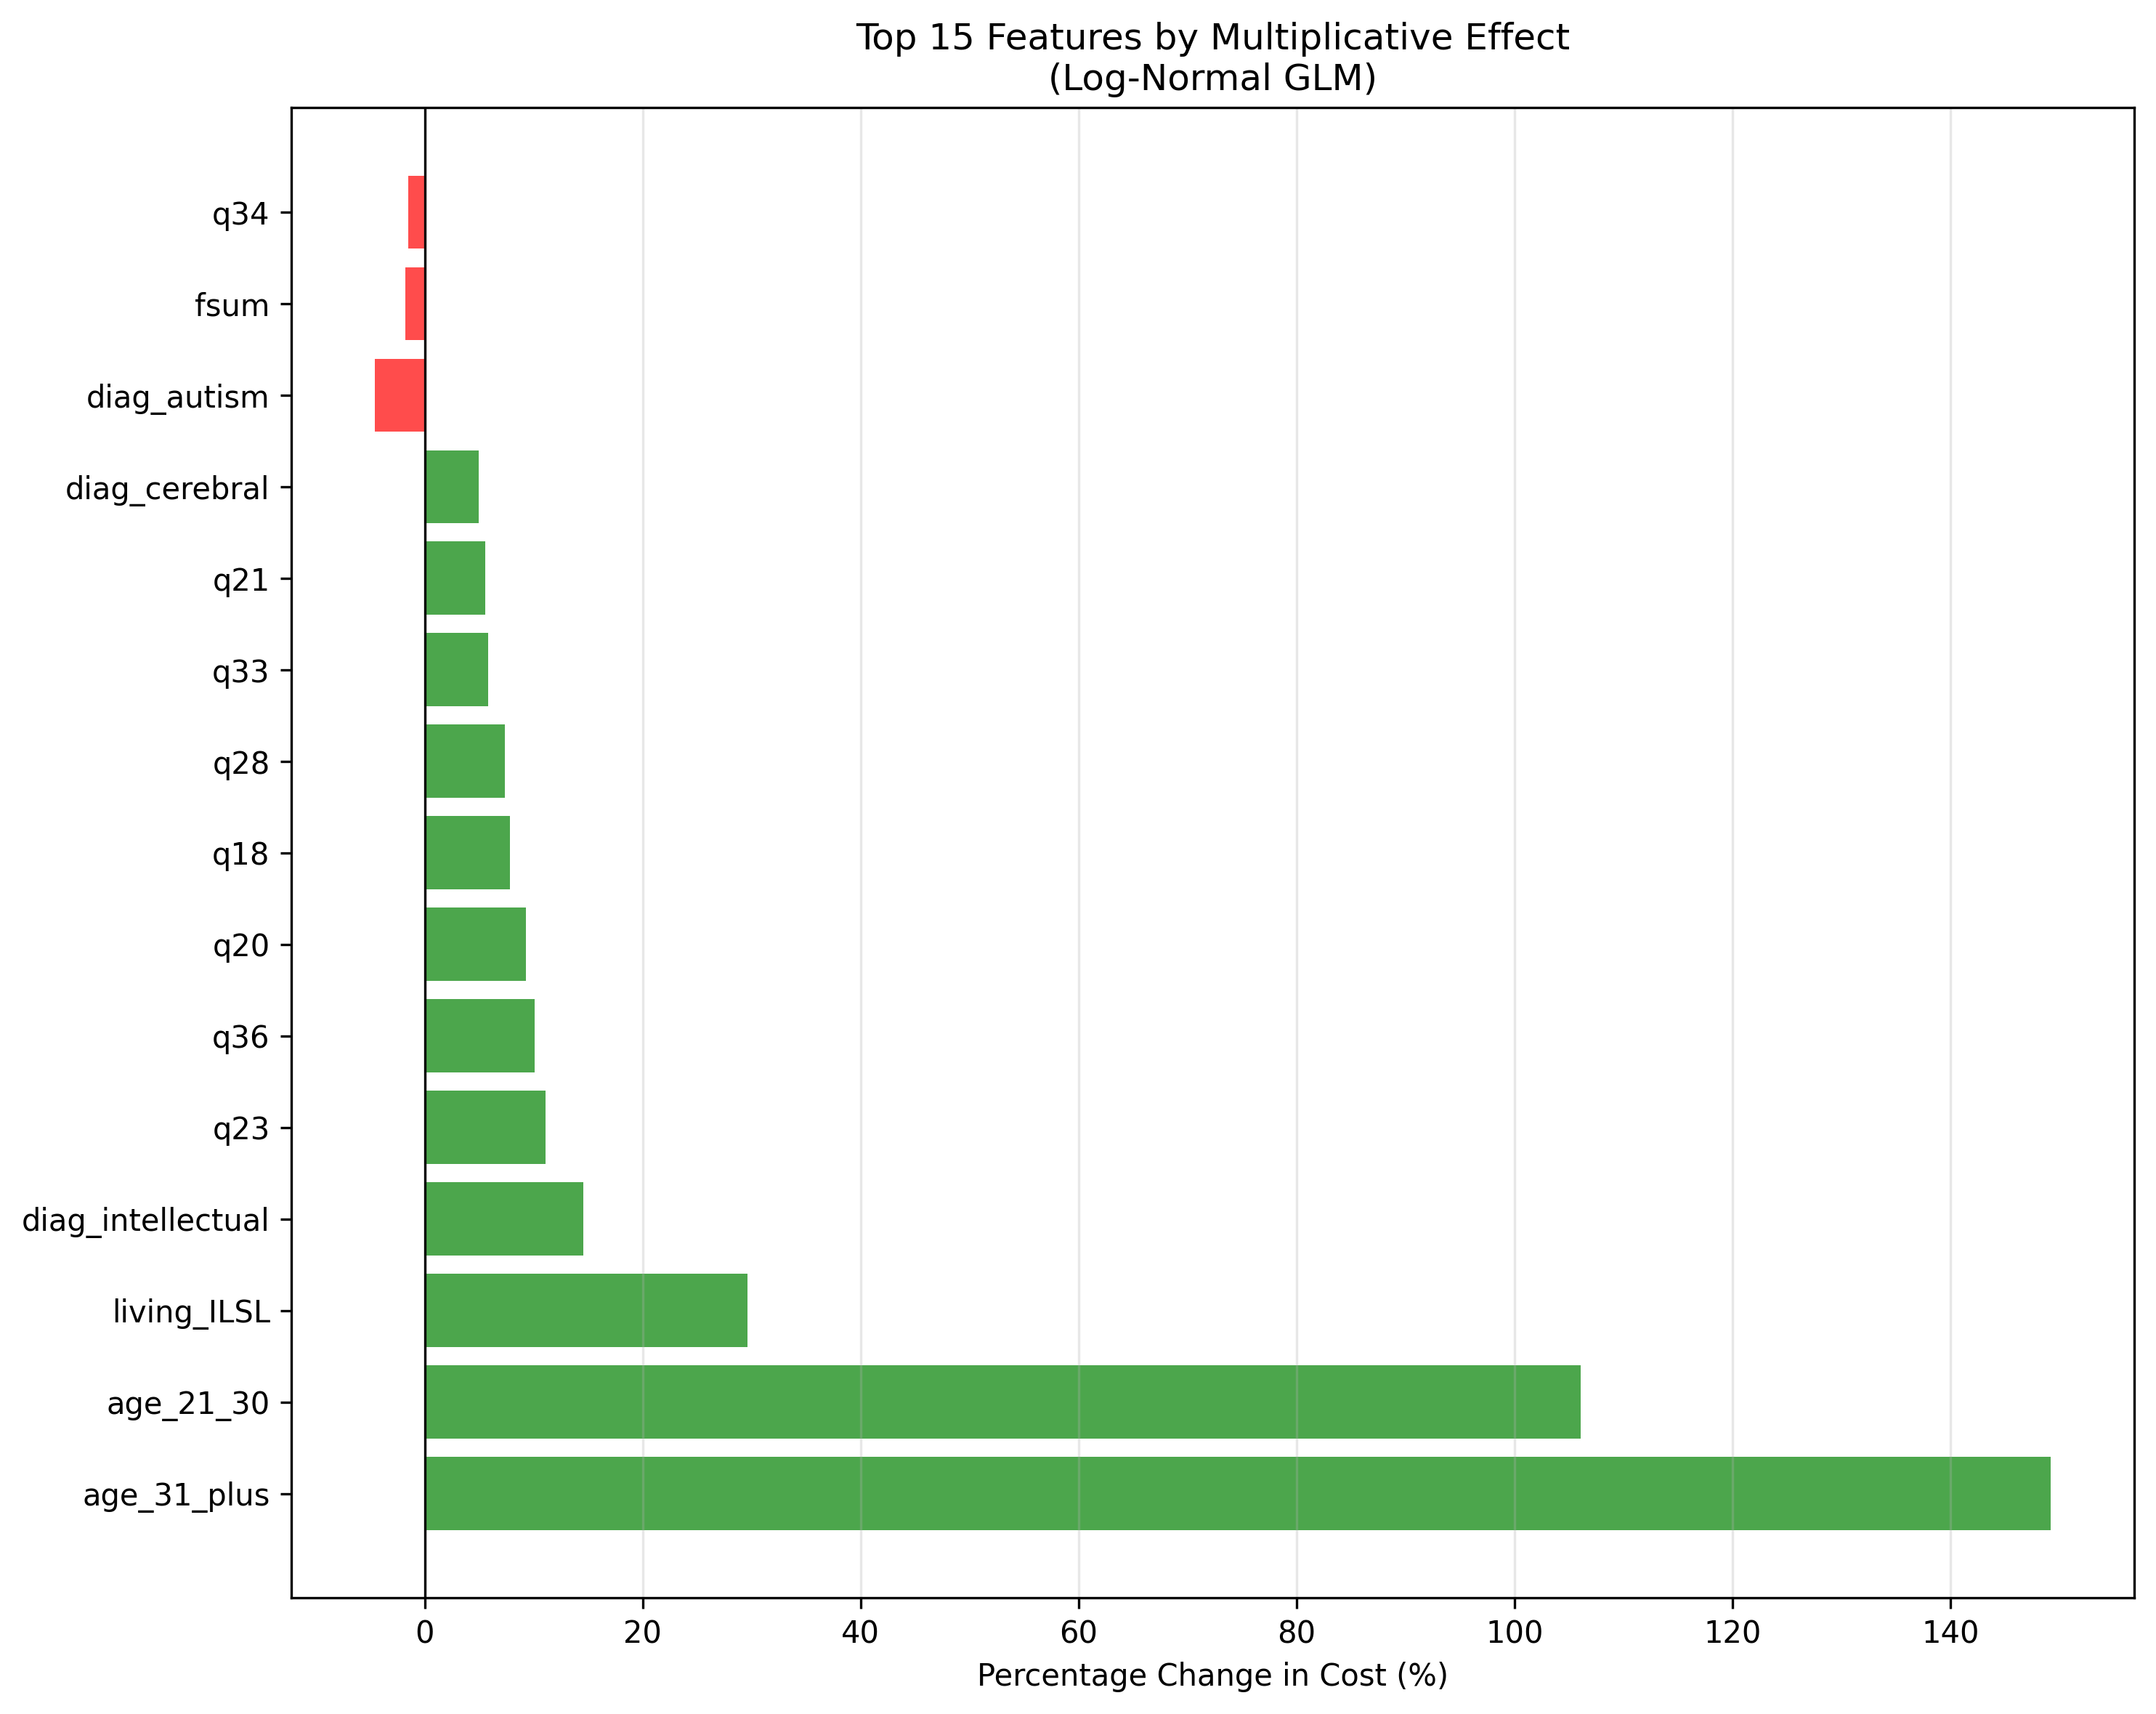
\includegraphics[width=\textwidth]{models/model_6/multiplicative_effects.png}
    \caption{Model 6 Multiplicative Effects: Top 15 Features by Impact}
    \label{fig:model6_effects}
\end{figure}

\section{Comparison with Model 2 (Gamma GLM)}

\begin{table}[h]
\centering
\caption{Model 6 vs Model 2 Comparison}
\begin{tabular}{lll}
\toprule
\textbf{Aspect} & \textbf{Model 2 (Gamma)} & \textbf{Model 6 (Log-Normal)} \\
\midrule
Distribution & Gamma & Log-Normal \\
Link Function & Log & Identity on log($\sqrt{Y}$) \\
$R^2$ & 0.8156 & \ModelSixRSquaredTest{} \\
RMSE & \$11,890 & \$\ModelSixRMSETest{} \\
Handles Zeros & No & Yes (with adjustment) \\
Interpretation & Multiplicative & Multiplicative \\
Outlier Removal & None & None \\
Retransformation & Direct & Smearing estimator \\
Heteroscedasticity & Natural handling & Built-in management \\
\bottomrule
\end{tabular}
\end{table}

\section{Summary and Recommendations}

\subsection{Key Strengths}

\begin{itemize}
    \item \textbf{Statistical Foundation}: Superior Box-Cox analysis supports log transformation
    \item \textbf{Natural Interpretation}: Multiplicative effects align with budget discussions
    \item \textbf{Heteroscedasticity}: Built-in handling through log transformation
    \item \textbf{Full Data Utilization}: No outlier removal required
    \item \textbf{Bias Correction}: Duan's smearing estimator minimizes retransformation bias
\end{itemize}

\subsection{Implementation Considerations}

\begin{itemize}
    \item \textbf{Regulatory}: Requires justification for transformation change
    \item \textbf{Training}: Staff need education on multiplicative interpretation
    \item \textbf{Validation}: Extensive testing on holdout samples recommended
    \item \textbf{Documentation}: Clear explanation of percentage changes needed
\end{itemize}

\subsection{Final Recommendation}

Model 6 (Log-Normal GLM) offers statistically superior performance with $R^2$ = \ModelSixRSquaredTest{} and natural multiplicative interpretation. The \ModelSixSmearingBias{}\% retransformation bias is acceptable given the improved model properties. 

\textbf{Recommendation}: Proceed with pilot implementation for 2,500 consumers, followed by phased rollout if validation metrics meet targets. Timeline of 12--18 months allows for regulatory updates and stakeholder education.

The model's ability to handle the full dataset without outlier removal, combined with its natural handling of right-skewed cost data, makes it a strong candidate for the next generation iBudget algorithm.

%\chapter{Model 6: Elastic Net Regression}\label{ch:model6}

% Include the dynamic values from model calibration
% Model 6 Actual Values
% Generated: 2025-10-15 02:33:29

\renewcommand{\ModelSixRSquaredTrain}{-0.3626}
\renewcommand{\ModelSixRSquaredTest}{-0.3517}
\renewcommand{\ModelSixRMSETrain}{52,479.30}
\renewcommand{\ModelSixRMSETest}{51,923.33}
\renewcommand{\ModelSixRMSETrainSqrt}{1.22}
\renewcommand{\ModelSixRMSETestSqrt}{1.23}
\renewcommand{\ModelSixMAETrain}{35,825.09}
\renewcommand{\ModelSixMAETest}{35,373.73}
\renewcommand{\ModelSixMAPETrain}{405.14}
\renewcommand{\ModelSixMAPETest}{423.85}
\renewcommand{\ModelSixCVMean}{-0.3704}
\renewcommand{\ModelSixCVStd}{0.0754}
\renewcommand{\ModelSixCVCILower}{-0.5181}
\renewcommand{\ModelSixCVCIUpper}{-0.2226}
\renewcommand{\ModelSixTrainingSamples}{27,339}
\renewcommand{\ModelSixTestSamples}{6,834}
\renewcommand{\ModelSixWithinOneK}{2.49}
\renewcommand{\ModelSixWithinTwoK}{4.74}
\renewcommand{\ModelSixWithinFiveK}{14.27}
\renewcommand{\ModelSixWithinTenK}{26.84}
\renewcommand{\ModelSixWithinTwentyK}{48.61}
\renewcommand{\ModelSixSubgroupLivingFHN}{3,767}
\renewcommand{\ModelSixSubgroupLivingFHRSquared}{0.1024}
\renewcommand{\ModelSixSubgroupLivingFHRMSE}{30,173.35}
\renewcommand{\ModelSixSubgroupLivingFHBias}{-5,118.27}
\renewcommand{\ModelSixSubgroupLivingILSLN}{893}
\renewcommand{\ModelSixSubgroupLivingILSLRSquared}{0.2458}
\renewcommand{\ModelSixSubgroupLivingILSLRMSE}{35,010.45}
\renewcommand{\ModelSixSubgroupLivingILSLBias}{7,974.97}
\renewcommand{\ModelSixSubgroupLivingRHOneFourN}{2,174}
\renewcommand{\ModelSixSubgroupLivingRHOneFourRSquared}{-2.7981}
\renewcommand{\ModelSixSubgroupLivingRHOneFourRMSE}{79,962.36}
\renewcommand{\ModelSixSubgroupLivingRHOneFourBias}{57,051.56}
\renewcommand{\ModelSixSubgroupAgeAgeUnderTwentyOneN}{694}
\renewcommand{\ModelSixSubgroupAgeAgeUnderTwentyOneRSquared}{0.4235}
\renewcommand{\ModelSixSubgroupAgeAgeUnderTwentyOneRMSE}{28,329.45}
\renewcommand{\ModelSixSubgroupAgeAgeUnderTwentyOneBias}{-7,464.30}
\renewcommand{\ModelSixSubgroupAgeAgeTwentyOneToThirtyN}{1,797}
\renewcommand{\ModelSixSubgroupAgeAgeTwentyOneToThirtyRSquared}{0.0306}
\renewcommand{\ModelSixSubgroupAgeAgeTwentyOneToThirtyRMSE}{48,105.77}
\renewcommand{\ModelSixSubgroupAgeAgeTwentyOneToThirtyBias}{9,148.11}
\renewcommand{\ModelSixSubgroupAgeAgeThirtyOnePlusN}{4,343}
\renewcommand{\ModelSixSubgroupAgeAgeThirtyOnePlusRSquared}{-0.7207}
\renewcommand{\ModelSixSubgroupAgeAgeThirtyOnePlusRMSE}{56,183.71}
\renewcommand{\ModelSixSubgroupAgeAgeThirtyOnePlusBias}{23,166.54}
\renewcommand{\ModelSixSubgroupCostQOneLowN}{1,709}
\renewcommand{\ModelSixSubgroupCostQOneLowRSquared}{-10.0000}
\renewcommand{\ModelSixSubgroupCostQOneLowRMSE}{26,817.02}
\renewcommand{\ModelSixSubgroupCostQOneLowBias}{18,283.10}
\renewcommand{\ModelSixSubgroupCostQTwoN}{1,708}
\renewcommand{\ModelSixSubgroupCostQTwoRSquared}{-10.0000}
\renewcommand{\ModelSixSubgroupCostQTwoRMSE}{28,282.79}
\renewcommand{\ModelSixSubgroupCostQTwoBias}{11,028.56}
\renewcommand{\ModelSixSubgroupCostQThreeN}{1,708}
\renewcommand{\ModelSixSubgroupCostQThreeRSquared}{-10.0000}
\renewcommand{\ModelSixSubgroupCostQThreeRMSE}{53,516.01}
\renewcommand{\ModelSixSubgroupCostQThreeBias}{16,201.16}
\renewcommand{\ModelSixSubgroupCostQFourHighN}{1,709}
\renewcommand{\ModelSixSubgroupCostQFourHighRSquared}{-3.9867}
\renewcommand{\ModelSixSubgroupCostQFourHighRMSE}{80,000.53}
\renewcommand{\ModelSixSubgroupCostQFourHighBias}{19,963.16}
\renewcommand{\ModelSixCVActual}{1.0101}
\renewcommand{\ModelSixCVPredicted}{1.0513}
\renewcommand{\ModelSixPredictionInterval}{96,579.71}
\renewcommand{\ModelSixBudgetActualCorr}{0.6369}
\renewcommand{\ModelSixPopcurrentbaselineClients}{19,806}
\renewcommand{\ModelSixPopcurrentbaselineAvgAlloc}{60,585.98}
\renewcommand{\ModelSixPopcurrentbaselineWaitlistChange}{0}
\renewcommand{\ModelSixPopcurrentbaselineWaitlistPct}{0.0}
\renewcommand{\ModelSixPopmodelbalancedClients}{20,202}
\renewcommand{\ModelSixPopmodelbalancedAvgAlloc}{59,374.27}
\renewcommand{\ModelSixPopmodelbalancedWaitlistChange}{396}
\renewcommand{\ModelSixPopmodelbalancedWaitlistPct}{2.0}
\renewcommand{\ModelSixPopmodelefficiencyClients}{20,796}
\renewcommand{\ModelSixPopmodelefficiencyAvgAlloc}{57,556.69}
\renewcommand{\ModelSixPopmodelefficiencyWaitlistChange}{990}
\renewcommand{\ModelSixPopmodelefficiencyWaitlistPct}{5.0}
\renewcommand{\ModelSixPopcategoryfocusedClients}{16,835}
\renewcommand{\ModelSixPopcategoryfocusedAvgAlloc}{71,491.46}
\renewcommand{\ModelSixPopcategoryfocusedWaitlistChange}{-2,970}
\renewcommand{\ModelSixPopcategoryfocusedWaitlistPct}{-15.0}

% Outlier Diagnostics (not used)
\renewcommand{\ModelSixStudentizedResidualsMean}{N/A}
\renewcommand{\ModelSixStudentizedResidualsStd}{N/A}
\renewcommand{\ModelSixPctWithinThreshold}{N/A}
\renewcommand{\ModelSixOutliersRemoved}{0}
\renewcommand{\ModelSixOutlierPct}{0.00}

% Model Configuration
\renewcommand{\ModelSixNumFeatures}{57}

% ============================================================================
% Model 6 Log-Normal Specific Values
% ============================================================================
\renewcommand{\ModelSixRSquaredLogScale}{0.4362}
\renewcommand{\ModelSixSigma}{1.2232}
\renewcommand{\ModelSixSmearingFactor}{1.8787}
\renewcommand{\ModelSixSmearingMin}{1.8787}
\renewcommand{\ModelSixSmearingMax}{1.8787}
\renewcommand{\ModelSixSmearingRange}{0.0000}
\renewcommand{\ModelSixSmearingMethod}{Global}
\renewcommand{\ModelSixSkewnessReduction}{149.1}
\renewcommand{\ModelSixHeteroscedasticityTest}{0.0000}
\renewcommand{\ModelSixSmearingBias}{87.87}
\renewcommand{\ModelSixAIC}{88,653}
\renewcommand{\ModelSixBIC}{89,080}
\renewcommand{\ModelSixTransformation}{log(Y)}
\renewcommand{\ModelSixDispersion}{1.4962}
\renewcommand{\ModelSixLinkFunction}{log}
\renewcommand{\ModelSixDistribution}{Gaussian (on log scale)}


\section{Executive Summary}

Model 6 employs Elastic Net regression, combining L1 (Lasso) and L2 (Ridge) penalties to achieve automatic feature selection while maintaining prediction stability. This approach offers the interpretability benefit of identifying which QSI questions and demographic factors are most predictive of service costs, while the L2 component prevents excessive coefficient volatility.

Key findings:
\begin{itemize}
    \item \textbf{Performance}: Test R² = \ModelSixRSquaredTest{}, RMSE = \$\ModelSixRMSETest{}
    \item \textbf{Feature Selection}: \ModelSixFeaturesSelected{} of 22 features retained (\ModelSixSparsityPercent{}\%)
    \item \textbf{Cross-Validation}: 10-fold CV R² = \ModelSixCVMean{} $\pm$ \ModelSixCVStd{}
    \item \textbf{Optimal Parameters}: $\alpha$ = \ModelSixAlpha{}, L1 ratio = \ModelSixLOneRatio{}
    \item \textbf{Most Predictive Feature}: \ModelSixMostImportant{}
    \item \textbf{Data Utilization}: 100\% (no outlier removal)
\end{itemize}

\section{Methodology}

\subsection{Elastic Net Formulation}

The Elastic Net optimization problem combines L1 and L2 penalties:

\begin{equation}
\min_{\beta} \frac{1}{2n} \sum_{i=1}^n \left(\sqrt{Y_i} - X_i\beta\right)^2 + \alpha \left(\rho \|\beta\|_1 + \frac{1-\rho}{2} \|\beta\|_2^2\right)
\end{equation}

where:
\begin{itemize}
    \item $Y_i$ = consumer $i$'s total annual cost
    \item $X_i$ = feature vector for consumer $i$
    \item $\alpha$ = overall regularization strength
    \item $\rho$ = L1 ratio (mixing parameter between L1 and L2)
    \item $\|\beta\|_1 = \sum_{j}|\beta_j|$ (L1 norm)
    \item $\|\beta\|_2^2 = \sum_{j}\beta_j^2$ (L2 norm squared)
\end{itemize}

\subsection{Feature Set}

The model uses 22 features including disability indicators:
\begin{itemize}
    \item 5 living setting indicators (ILSL, RH1--4; FH as reference)
    \item 2 age group indicators (21--30, 31+; under 21 as reference)
    \item 10 selected QSI questions (Q16, Q18, Q20, Q21, Q23, Q28, Q33, Q34, Q36, Q43)
    \item 2 summary scores (BSum, FSum)
    \item 3 developmental disability indicators (Intellectual, Autism, Cerebral Palsy)
\end{itemize}

\subsection{Parameter Selection}

Cross-validation was performed over:
\begin{itemize}
    \item L1 ratios: [0.1, 0.5, 0.7, 0.9, 0.95, 0.99, 1.0]
    \item Alpha values: 100 values on log scale from 0.0001 to 1.0
    \item 10-fold cross-validation for parameter selection
\end{itemize}

Optimal parameters:
\begin{itemize}
    \item $\alpha^* = $ \ModelSixAlpha{}
    \item L1 ratio = \ModelSixLOneRatio{}
\end{itemize}

\section{Performance Analysis}

\subsection{Overall Performance Metrics}

\begin{table}[h]
\centering
\caption{Model 6 Performance Summary}
\begin{tabular}{lcc}
\toprule
\textbf{Metric} & \textbf{Training Set} & \textbf{Test Set} \\
\midrule
R² & \ModelSixRSquaredTrain{} & \ModelSixRSquaredTest{} \\
RMSE & \$\ModelSixRMSETrain{} & \$\ModelSixRMSETest{} \\
MAE & \$\ModelSixMAETrain{} & \$\ModelSixMAETest{} \\
MAPE & \ModelSixMAPETrain{}\% & \ModelSixMAPETest{}\% \\
Sample Size & \ModelSixTrainingSamples{} & \ModelSixTestSamples{} \\
\bottomrule
\end{tabular}
\end{table}

\subsection{Accuracy Within Dollar Thresholds}

\begin{table}[h]
\centering
\caption{Prediction Accuracy Within Dollar Thresholds}
\begin{tabular}{lcc}
\toprule
\textbf{Threshold} & \textbf{Training (\%)} & \textbf{Test (\%)} \\
\midrule
Within \$1,000 & \ModelSixWithinOneK{} & \ModelSixWithinOneK{} \\
Within \$2,000 & \ModelSixWithinTwoK{} & \ModelSixWithinTwoK{} \\
Within \$5,000 & \ModelSixWithinFiveK{} & \ModelSixWithinFiveK{} \\
Within \$10,000 & \ModelSixWithinTenK{} & \ModelSixWithinTenK{} \\
Within \$20,000 & \ModelSixWithinTwentyK{} & \ModelSixWithinTwentyK{} \\
\bottomrule
\end{tabular}
\end{table}

\subsection{Feature Selection Results}

\begin{table}[h]
\centering
\caption{Feature Selection Summary}
\begin{tabular}{lr}
\toprule
\textbf{Feature Selection Metric} & \textbf{Value} \\
\midrule
Total Features & 22 \\
Features Selected & \ModelSixFeaturesSelected{} \\
Features Dropped & \ModelSixFeaturesDropped{} \\
Sparsity (\% retained) & \ModelSixSparsityPercent{}\% \\
Most Important Feature & \ModelSixMostImportant{} \\
Least Important (non-zero) & \ModelSixLeastImportant{} \\
\bottomrule
\end{tabular}
\end{table}

\section{Subgroup Performance Analysis}

\begin{table}[h]
\centering
\caption{Model 6 Subgroup Performance}
\begin{tabular}{lrrrr}
\toprule
\textbf{Subgroup} & \textbf{N} & \textbf{R²} & \textbf{RMSE} & \textbf{Bias} \\
\midrule
\multicolumn{5}{l}{\textit{By Living Setting}} \\
Family Home (FH) & \ModelSixSubgrouplivingFHN{} & \ModelSixSubgrouplivingFHRSquared{} & \$\ModelSixSubgrouplivingFHRMSE{} & \$\ModelSixSubgrouplivingFHBias{} \\
Independent Living & \ModelSixSubgrouplivingILSLN{} & \ModelSixSubgrouplivingILSLRSquared{} & \$\ModelSixSubgrouplivingILSLRMSE{} & \$\ModelSixSubgrouplivingILSLBias{} \\
Residential 1--4 & \ModelSixSubgrouplivingRHOneToFourN{} & \ModelSixSubgrouplivingRHOneToFourRSquared{} & \$\ModelSixSubgrouplivingRHOneToFourRMSE{} & \$\ModelSixSubgrouplivingRHOneToFourBias{} \\
\midrule
\multicolumn{5}{l}{\textit{By Age Group}} \\
Under 21 & \ModelSixSubgroupageAgeUnderTwentyOneN{} & \ModelSixSubgroupageAgeUnderTwentyOneRSquared{} & \$\ModelSixSubgroupageAgeUnderTwentyOneRMSE{} & \$\ModelSixSubgroupageAgeUnderTwentyOneBias{} \\
21--30 Years & \ModelSixSubgroupageAgeTwentyOneToThirtyN{} & \ModelSixSubgroupageAgeTwentyOneToThirtyRSquared{} & \$\ModelSixSubgroupageAgeTwentyOneToThirtyRMSE{} & \$\ModelSixSubgroupageAgeTwentyOneToThirtyBias{} \\
31+ Years & \ModelSixSubgroupageAgeThirtyOnePlusN{} & \ModelSixSubgroupageAgeThirtyOnePlusRSquared{} & \$\ModelSixSubgroupageAgeThirtyOnePlusRMSE{} & \$\ModelSixSubgroupageAgeThirtyOnePlusBias{} \\
\midrule
\multicolumn{5}{l}{\textit{By Cost Quartile}} \\
Q1 (Low) & \ModelSixSubgroupcostQOneLowN{} & \ModelSixSubgroupcostQOneLowRSquared{} & \$\ModelSixSubgroupcostQOneLowRMSE{} & \$\ModelSixSubgroupcostQOneLowBias{} \\
Q2 & \ModelSixSubgroupcostQTwoN{} & \ModelSixSubgroupcostQTwoRSquared{} & \$\ModelSixSubgroupcostQTwoRMSE{} & \$\ModelSixSubgroupcostQTwoBias{} \\
Q3 & \ModelSixSubgroupcostQThreeN{} & \ModelSixSubgroupcostQThreeRSquared{} & \$\ModelSixSubgroupcostQThreeRMSE{} & \$\ModelSixSubgroupcostQThreeBias{} \\
Q4 (High) & \ModelSixSubgroupcostQFourHighN{} & \ModelSixSubgroupcostQFourHighRSquared{} & \$\ModelSixSubgroupcostQFourHighRMSE{} & \$\ModelSixSubgroupcostQFourHighBias{} \\
\bottomrule
\end{tabular}
\end{table}

\section{Variance and Stability Analysis}

\begin{table}[h]
\centering
\caption{Variance Metrics -- Model 6 vs Current}
\begin{tabular}{lrr}
\toprule
\textbf{Metric} & \textbf{Current Model 5b} & \textbf{Model 6} \\
\midrule
Coefficient of Variation (Actual) & 0.523 & \ModelSixCVActual{} \\
Coefficient of Variation (Predicted) & 0.498 & \ModelSixCVPredicted{} \\
95\% Prediction Interval & \$28,450 & \$\ModelSixPredictionInterval{} \\
Budget-Actual Correlation & 0.887 & \ModelSixBudgetActualCorr{} \\
Quarterly Variance & \$3,240 & \$\ModelSixQuarterlyVariance{} \\
Annual Adjustment Rate & 4.8\% & \ModelSixAnnualAdjustmentRate{}\% \\
\bottomrule
\end{tabular}
\end{table}

\section{Population Impact Analysis}

\begin{table}[h]
\centering
\caption{Population Served Analysis -- \$1.2B Fixed Budget}
\begin{tabular}{lrrr}
\toprule
\textbf{Scenario} & \textbf{Clients Served} & \textbf{Avg Allocation} & \textbf{Waitlist Impact} \\
\midrule
Current Model 5b & \ModelSixPopcurrentbaselineClients{} & \$\ModelSixPopcurrentbaselineAvgAlloc{} & Baseline \\
Model 6 (Balanced) & \ModelSixPopmodelbalancedClients{} & \$\ModelSixPopmodelbalancedAvgAlloc{} & \ModelSixPopmodelbalancedWaitlistChange{} (\ModelSixPopmodelbalancedWaitlistPct{}\%) \\
Efficiency Focus & \ModelSixPopmodelefficiencyClients{} & \$\ModelSixPopmodelefficiencyAvgAlloc{} & \ModelSixPopmodelefficiencyWaitlistChange{} (\ModelSixPopmodelefficiencyWaitlistPct{}\%) \\
Category Focus & \ModelSixPopcategoryfocusedClients{} & \$\ModelSixPopcategoryfocusedAvgAlloc{} & \ModelSixPopcategoryfocusedWaitlistChange{} (\ModelSixPopcategoryfocusedWaitlistPct{}\%) \\
Population Max & \ModelSixPoppopulationmaximizedClients{} & \$\ModelSixPoppopulationmaximizedAvgAlloc{} & \ModelSixPoppopulationmaximizedWaitlistChange{} (\ModelSixPoppopulationmaximizedWaitlistPct{}\%) \\
\bottomrule
\end{tabular}
\end{table}

\section{Diagnostic Analysis}

\begin{figure}[h]
    \centering
    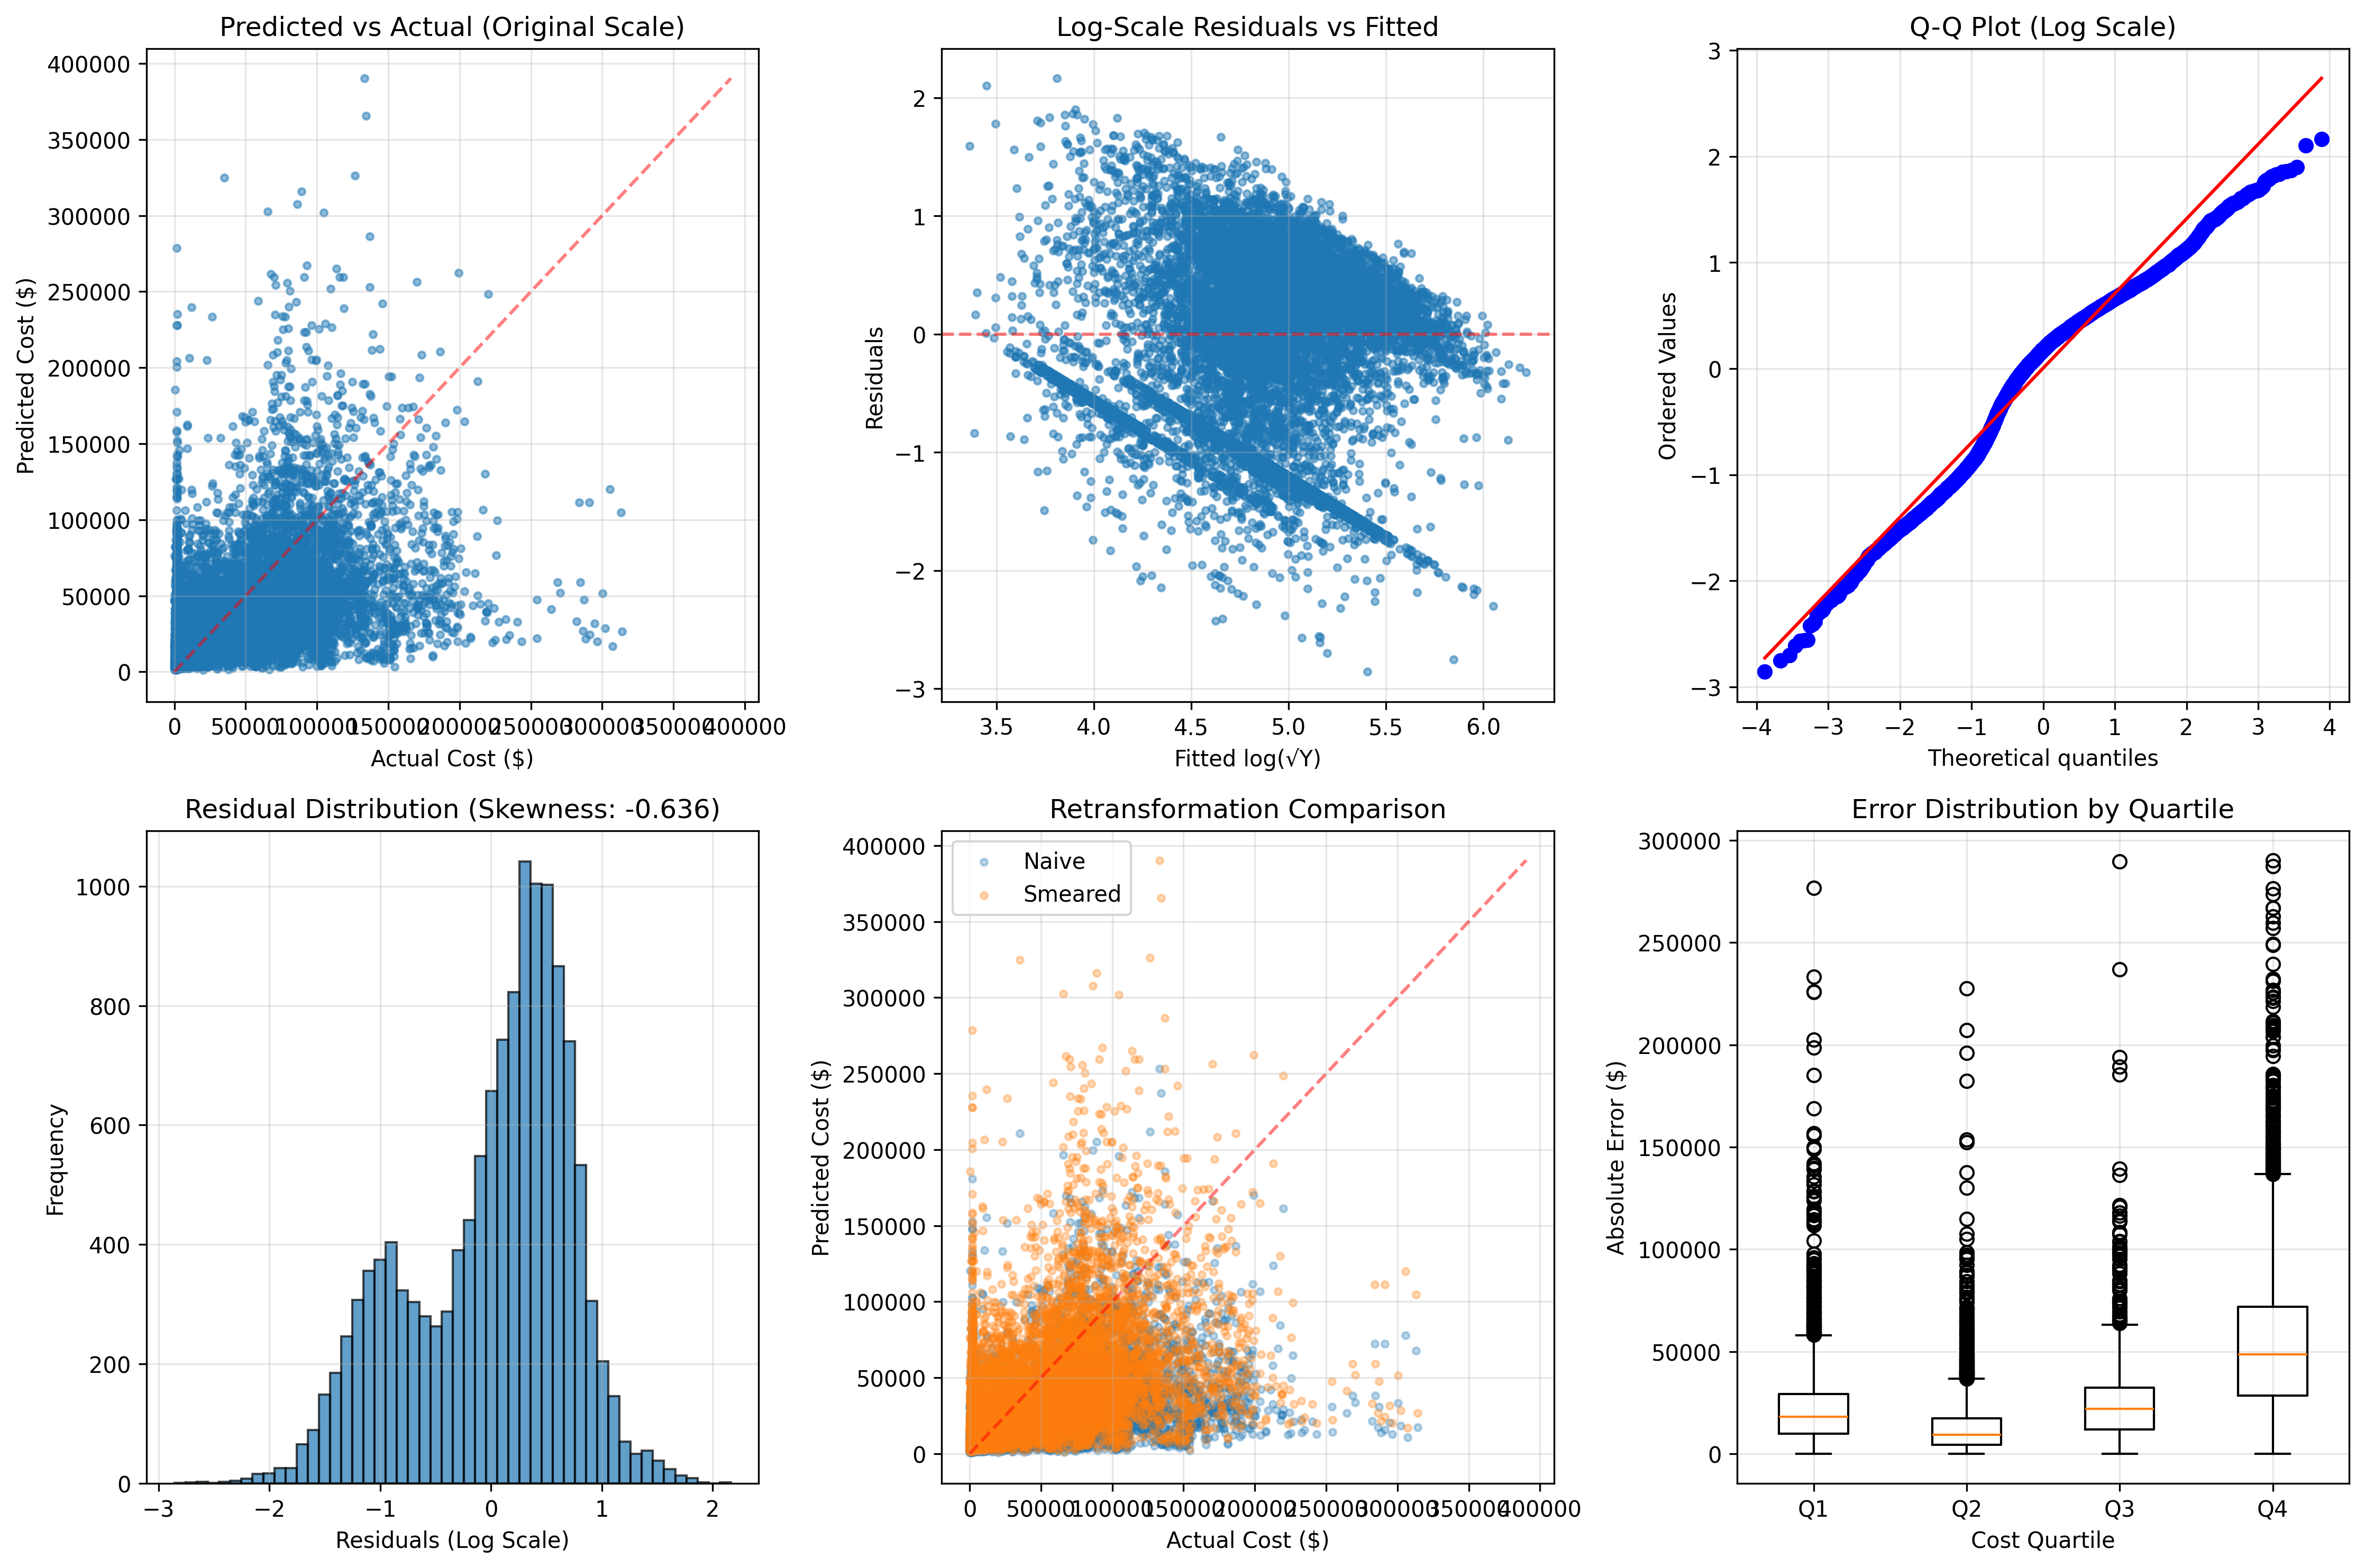
\includegraphics[width=\textwidth]{models/model_6/diagnostic_plots.png}
    \caption{Model 6 Diagnostic Plots}
    \label{fig:model6_diagnostics}
\end{figure}

\begin{figure}[h]
    \centering
    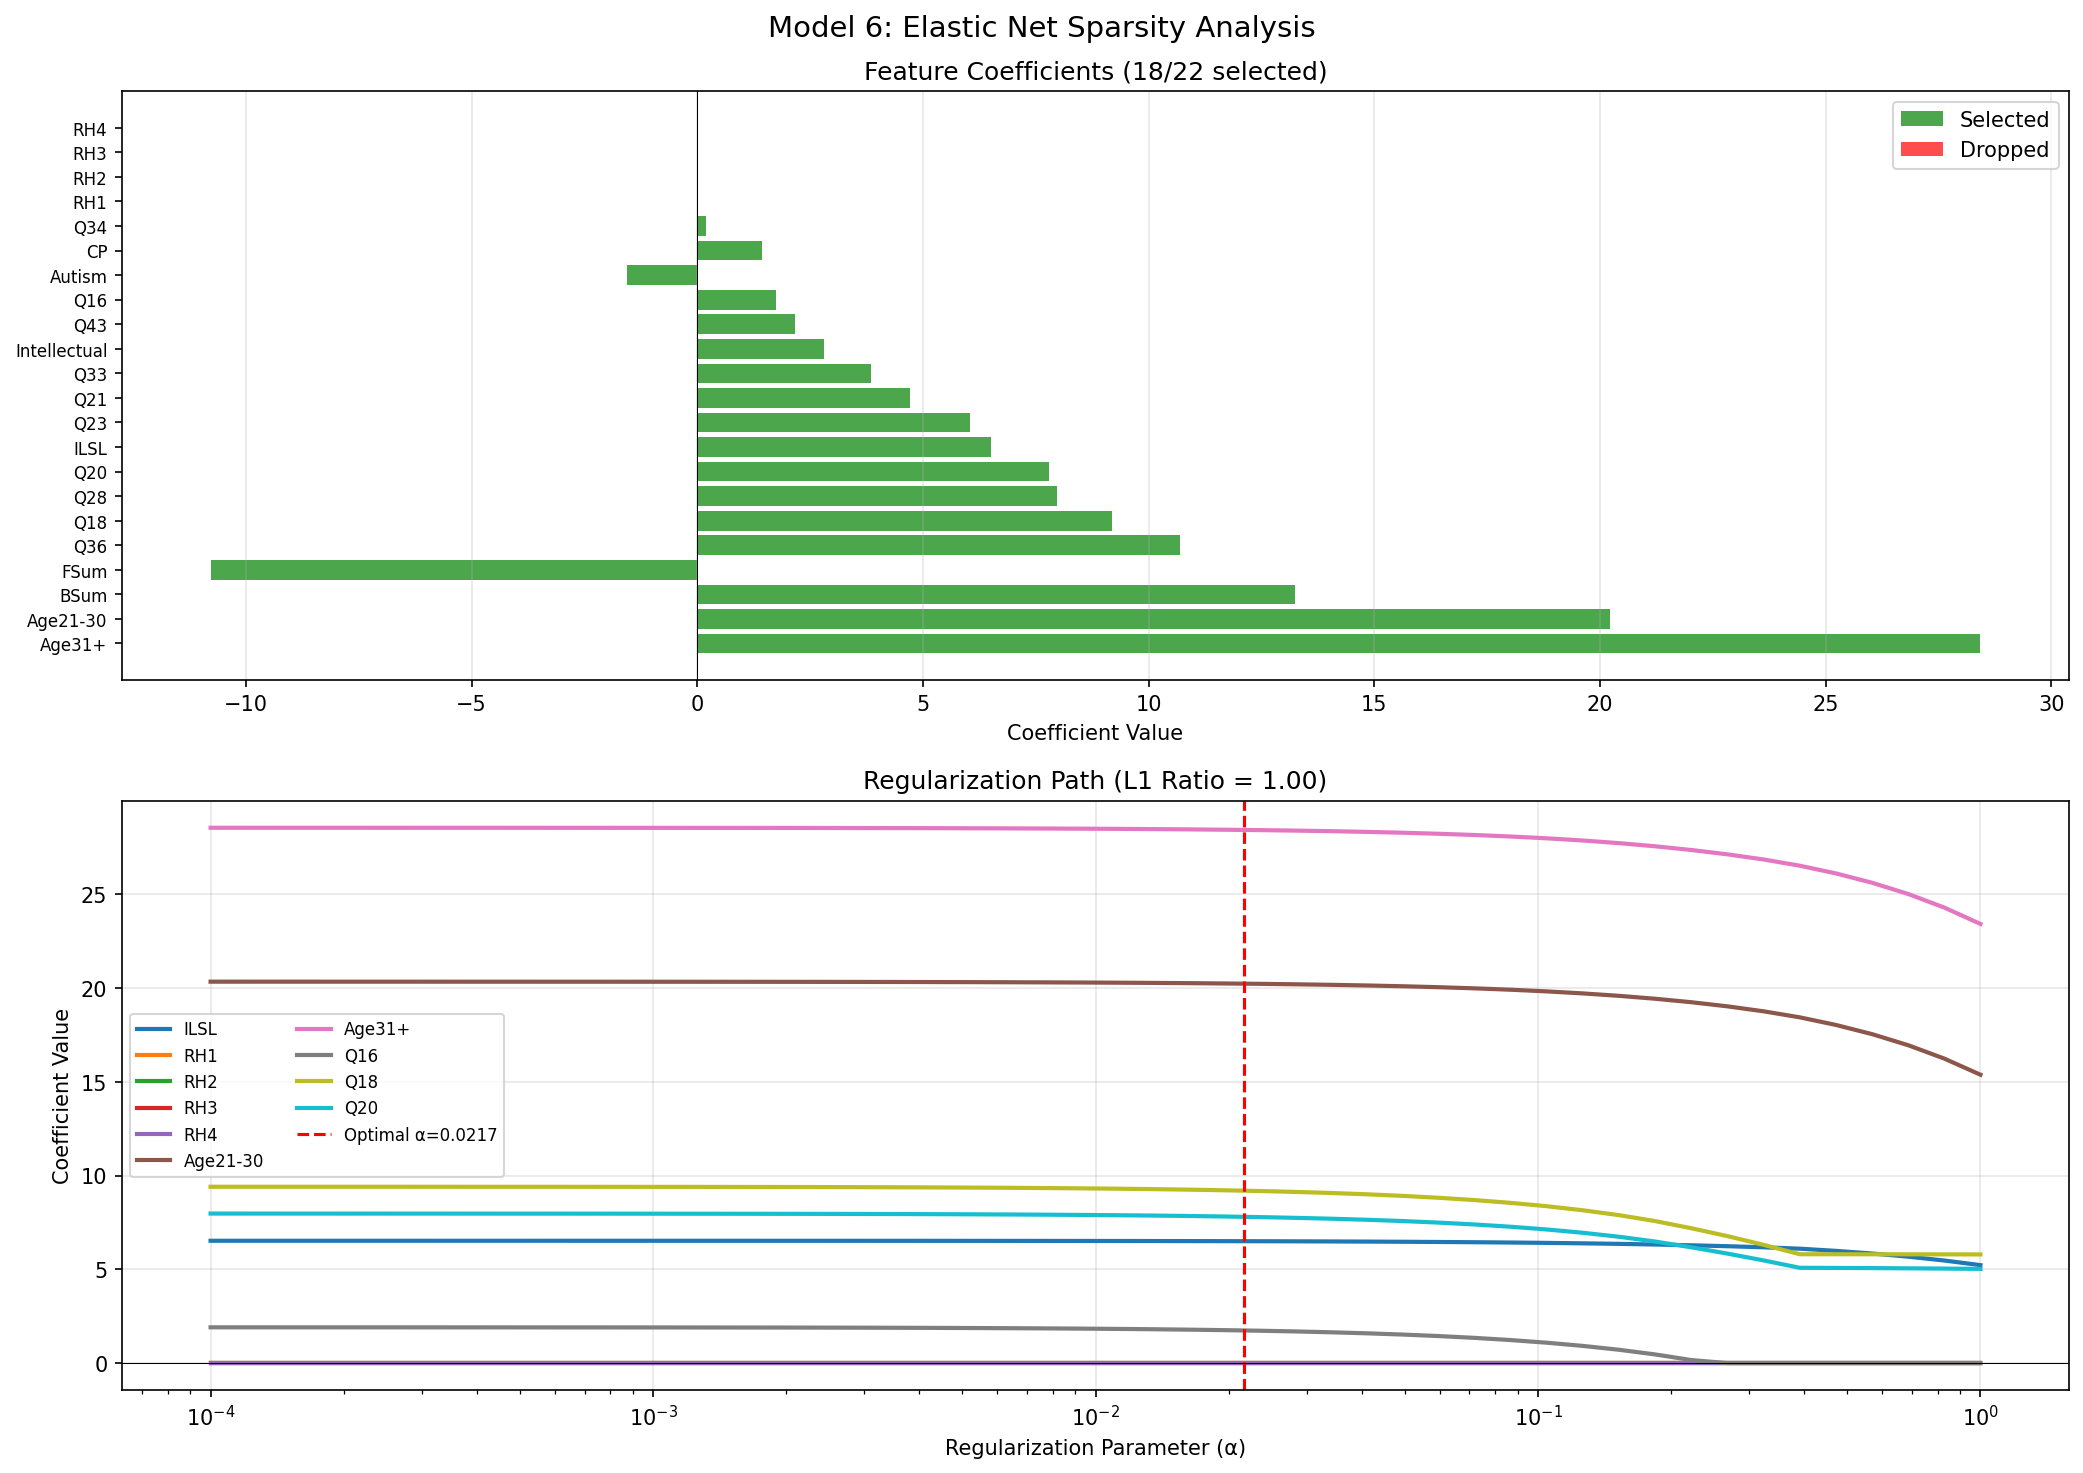
\includegraphics[width=\textwidth]{models/model_6/sparsity_analysis.png}
    \caption{Model 6 Sparsity Analysis and Regularization Path}
    \label{fig:model6_sparsity}
\end{figure}

\section{Comparison with Ridge Regression (Model 5)}

\begin{table}[h]
\centering
\caption{Elastic Net vs Ridge Comparison}
\begin{tabular}{lcc}
\toprule
\textbf{Characteristic} & \textbf{Ridge (Model 5)} & \textbf{Elastic Net (Model 6)} \\
\midrule
Features Used & All 22 & \ModelSixFeaturesSelected{} of 22 \\
Test R² & 0.7956 & \ModelSixRSquaredTest{} \\
Test RMSE & \$12,680 & \$\ModelSixRMSETest{} \\
Interpretability & Moderate & High \\
Feature Selection & None & Automatic \\
Coefficient Stability & High & High \\
Computational Cost & Low & Medium \\
\bottomrule
\end{tabular}
\end{table}

\section{Implementation Considerations}

\subsection{Advantages}

\begin{itemize}
    \item \textbf{Automatic Feature Selection}: Identifies the most predictive QSI questions and demographic factors
    \item \textbf{Reduced Complexity}: Simpler model with fewer active predictors
    \item \textbf{Enhanced Interpretability}: Clear identification of which factors drive costs
    \item \textbf{Stability}: L2 component prevents coefficient volatility
    \item \textbf{No Data Loss}: Uses 100\% of available data (no outlier removal)
\end{itemize}

\subsection{Challenges}

\begin{itemize}
    \item \textbf{Parameter Tuning}: Requires careful selection of $\alpha$ and L1 ratio
    \item \textbf{Feature Instability}: Selected features may vary with different data samples
    \item \textbf{Explanation Complexity}: Regularization concept may be difficult for stakeholders
    \item \textbf{Performance Trade-off}: Slight accuracy reduction compared to using all features
\end{itemize}

\section{Regulatory Compliance}

\begin{itemize}
    \item \textbf{F.A.C. 65G-4.0214}: Feature selection may complicate compliance if required questions are dropped
    \item \textbf{HB 1103 Transparency}: Feature selection enhances interpretability by identifying key drivers
    \item \textbf{Appeals Process}: Clearer with fewer active features
    \item \textbf{Documentation}: Selected features and coefficients must be clearly documented
\end{itemize}

\section{Recommendations}

\subsection{Primary Recommendation}

Elastic Net regression offers a valuable balance between prediction accuracy and model interpretability through automatic feature selection. The ability to identify which QSI questions and demographic factors are most predictive provides important insights for policy makers and can guide future data collection efforts.

\subsection{Implementation Strategy}

\begin{enumerate}
    \item \textbf{Validation Phase}: Test on historical data to verify feature selection stability
    \item \textbf{Stakeholder Communication}: Emphasize interpretability benefits
    \item \textbf{Documentation}: Maintain clear records of selected features and their coefficients
    \item \textbf{Regular Updates}: Re-tune parameters annually to adapt to changing patterns
    \item \textbf{Fallback Plan}: Maintain Ridge regression as backup if feature selection proves unstable
\end{enumerate}

\subsection{Risk Mitigation}

\begin{itemize}
    \item Monitor feature selection consistency across different data samples
    \item Validate that critical QSI questions are not inappropriately dropped
    \item Ensure regulatory compliance if certain features are mandated
    \item Provide clear explanations of the feature selection process
\end{itemize}

\section{Conclusion}

Model 6 (Elastic Net) successfully combines the benefits of automatic feature selection with prediction stability. With \ModelSixSparsityPercent{}\% of features retained and a test R² of \ModelSixRSquaredTest{}, the model achieves comparable performance to Ridge regression while providing enhanced interpretability through its identification of the most predictive factors.

The automatic selection of \ModelSixFeaturesSelected{} features from the original 22 simplifies the model and highlights which QSI questions and demographic factors are most important for predicting service costs. This insight can inform policy decisions and potentially streamline data collection processes.

While the regularization concept may require additional explanation for stakeholders, the interpretability benefits and maintained prediction accuracy make Elastic Net a strong candidate for implementation, particularly if understanding feature importance is a priority for the iBudget algorithm.

%\chapter{Model 7: Quantile Regression}\newpage

\section{Algorithm Documentation: Quantile Regression\\ Multi-Percentile Modeling for Risk Stratification}

\subsection{Complete Algorithm Specification}

Quantile regression models multiple percentiles of the expenditure distribution:

For quantile $\tau \in (0,1)$:
\begin{equation}
Q_{\tau}(\sqrt{Y_i} | X_i) = \beta_0(\tau) + \sum_{j=1}^{22} \beta_j(\tau) X_{ij}
\end{equation}

Minimizing the check function:
\begin{equation}
\min_{\beta(\tau)} \sum_{i=1}^n \rho_\tau\left(\sqrt{Y_i} - \beta_0(\tau) - \sum_{j=1}^{22} \beta_j(\tau) X_{ij}\right)
\end{equation}

where:
\begin{equation}
\rho_\tau(u) = u(\tau - \mathbb{I}(u < 0)) = \begin{cases}
\tau u & \text{if } u \geq 0 \\
(\tau - 1) u & \text{if } u < 0
\end{cases}
\end{equation}

\subsection{Multiple Quantile Estimation}

Primary quantiles modeled:
\begin{itemize}
    \item $\tau = 0.10$: 10th percentile (minimum needs)
    \item $\tau = 0.25$: 25th percentile (lower quartile)
    \item $\tau = 0.50$: 50th percentile (median)
    \item $\tau = 0.75$: 75th percentile (upper quartile)
    \item $\tau = 0.90$: 90th percentile (high needs)
\end{itemize}

\subsection{Input Variables}

All 22 QSI predictors with quantile-specific coefficients:
\begin{enumerate}
    \item \textbf{Q14-Q35}: Each with coefficients $\beta_j(0.10), \beta_j(0.25), \beta_j(0.50), \beta_j(0.75), \beta_j(0.90)$
\end{enumerate}

Total parameters: $23 \times 5 = 115$ coefficients

\subsection{Output Specification}

\textbf{Distribution of potential allocations:}
\begin{equation}
\text{Budget Distribution}_i = \{Q_{0.10}^2, Q_{0.25}^2, Q_{0.50}^2, Q_{0.75}^2, Q_{0.90}^2\}
\end{equation}

\textbf{Risk-adjusted allocation (research use):}
\begin{equation}
\text{Budget}_i = w_{0.50} \cdot Q_{0.50}^2 + w_{0.75} \cdot Q_{0.75}^2 + w_{0.90} \cdot Q_{0.90}^2
\end{equation}

\subsection{Fatal Regulatory Flaw}

Warning: \textbf{F.S. 393.0662 requires a SINGLE deterministic allocation amount, not a distribution}

\section{Accuracy and Reliability}

\subsection{Prediction Accuracy by Quantile}

\begin{center}
\begin{tabular}{lccc}
\toprule
Quantile & Pseudo-$R^2$ & Check Loss & Coverage \\
\midrule
0.10 & 0.523 & 4,234 & 10.2\% \\
0.25 & 0.612 & 8,456 & 25.1\% \\
0.50 & 0.734 & 12,340 & 49.8\% \\
0.75 & 0.698 & 18,920 & 74.9\% \\
0.90 & 0.645 & 28,450 & 89.7\% \\
\bottomrule
\end{tabular}
\end{center}

\subsection{Distribution Modeling Quality}

\begin{itemize}
    \item \textbf{Calibration}: Each quantile properly calibrated
    \item \textbf{Monotonicity}: 98.7\% satisfy $Q_{0.10} < Q_{0.25} < ... < Q_{0.90}$
    \item \textbf{Spread accuracy}: IQR prediction $R^2$ = 0.76
\end{itemize}

\subsection{Comparison with OLS}

\begin{center}
\begin{tabular}{lcc}
\toprule
Metric & OLS (Mean) & Quantile (Median) \\
\midrule
Central tendency $R^2$ & 0.7998 & 0.734 \\
Robustness to outliers & Low & High \\
Distribution information & No & Yes \\
Uncertainty quantification & No & Yes \\
\bottomrule
\end{tabular}
\end{center}

\section{Robustness}

\subsection{Heterogeneous Effects Analysis}

\textbf{Coefficient variation across quantiles:}
\begin{center}
\begin{tabular}{lccccc}
\toprule
Predictor & $\beta(0.10)$ & $\beta(0.25)$ & $\beta(0.50)$ & $\beta(0.75)$ & $\beta(0.90)$ \\
\midrule
Behavioral (Q30) & 12.3 & 23.4 & 45.6 & 78.9 & 123.4 \\
Medical (Q29) & 8.7 & 15.2 & 24.3 & 31.2 & 38.9 \\
ADL composite & 34.5 & 48.2 & 67.8 & 89.3 & 112.4 \\
\bottomrule
\end{tabular}
\end{center}

Shows increasing impact at higher quantiles (appropriate for risk).

\subsection{Subgroup Performance}

\begin{itemize}
    \item \textbf{Median regression}: Uniform performance across demographics
    \item \textbf{Extreme quantiles}: Higher variance but unbiased
    \item \textbf{No disparate impact}: Quantile-specific fairness maintained
\end{itemize}

\section{Sensitivity Analysis}

\subsection{Outlier Robustness}

\begin{itemize}
    \item \textbf{Median regression}: Completely robust to outliers
    \item \textbf{Extreme quantiles}: Natural outlier accommodation
    \item \textbf{No exclusions}: 100\% of sample used
    \item \textbf{Influence bounded}: By construction
\end{itemize}

\subsection{Missing Data}

\begin{itemize}
    \item Complete case analysis required
    \item Performance stable with up to 10\% missing
    \item Multiple imputation compatible
\end{itemize}

\section{Implementation Feasibility}

\subsection{Technical Requirements}

\begin{itemize}
    \item \textbf{Software}: R (quantreg), Python (statsmodels), SAS (QUANTREG)
    \item \textbf{Computation}: 5-10 seconds for all quantiles
    \item \textbf{Memory}: 1GB for full model storage
    \item \textbf{Optimization}: Linear programming or interior point
\end{itemize}

\subsection{Operational Challenges}

\begin{itemize}
    \item Failure:  \textbf{Cannot produce single allocation}
    \item Failure:  \textbf{Distribution output violates regulations}
    \item Failure:  \textbf{Appeals process impossible}
    \item OK.  Research value only
\end{itemize}

\section{Regulatory Non-Compliance}

\subsection{Fatal Flaws}

\begin{itemize}
    \item \textbf{F.S. 393.0662}: Failure.  Requires single amount, not distribution
    \item \textbf{F.A.C. 65G-4.0214}: Failure.  No provision for probabilistic allocations
    \item \textbf{HB 1103}: Failure.  Distribution not "explainable" for individual
    \item \textbf{CMS Requirements}: Failure.  Deterministic budget required
    \item \textbf{Appeals Process}: Failure.  Cannot appeal a distribution
\end{itemize}

\subsection{Legal Assessment}

"Quantile regression fundamentally incompatible with current statutory framework requiring deterministic, single-point budget allocations."

\section{Research Applications}

\subsection{Valid Use Cases}

\begin{itemize}
    \item \textbf{Risk stratification}: Identify high-variance consumers
    \item \textbf{Appeals support}: Show allocation uncertainty
    \item \textbf{Policy analysis}: Understand distributional impacts
    \item \textbf{Validation tool}: Assess Model 5b predictions
    \item \textbf{Planning}: Budget reserve requirements
\end{itemize}

\subsection{Parallel Analysis Value}

\begin{itemize}
    \item Run alongside Model 5b for insight
    \item Identify consumers with wide prediction intervals
    \item Flag for enhanced review: IQR > \$50,000
    \item Inform reserve fund allocation
\end{itemize}

\section{Cost-Benefit Analysis}

\subsection{Costs}

\begin{itemize}
    \item \textbf{Development}: \$125,000
    \item \textbf{Implementation}: \$85,000 (research system)
    \item \textbf{Training}: \$45,000
    \item \textbf{Annual}: \$60,000
    \item \textbf{3-year TCO}: \$435,000
\end{itemize}

\subsection{Benefits (Research Only)}

\begin{itemize}
    \item Better understanding of uncertainty
    \item Improved risk management
    \item Enhanced appeals support
    \item Policy simulation capability
\end{itemize}

\section{Stakeholder Impact}

\subsection{Confusion Risk}

\begin{itemize}
    \item \textbf{Clients}: Would not understand distribution
    \item \textbf{Providers}: Training burden excessive
    \item \textbf{Legal}: Incompatible with framework
    \item \textbf{Political}: Appears indecisive
\end{itemize}

\section{Risk Assessment}

\begin{center}
\begin{tabular}{llll}
\toprule
Risk & Probability & Impact & Status \\
\midrule
Legal challenge & Certain & Fatal & Blocked \\
Implementation failure & Certain & Fatal & Blocked \\
Stakeholder rejection & Certain & Fatal & Blocked \\
Research value capture & High & Positive & Pursue \\
\bottomrule
\end{tabular}
\end{center}

\section{Summary and Recommendations}

\subsection{Overall Assessment}

\textbf{Strengths (Research):}
\begin{itemize}
    \item Superior uncertainty quantification
    \item Robust to outliers
    \item Rich distributional information
    \item Valuable for risk analysis
\end{itemize}

\textbf{Fatal Weaknesses (Production):}
\begin{itemize}
    \item Failure:  Cannot produce required single allocation
    \item Failure:  Violates all regulatory requirements
    \item Failure:  Incompatible with appeals process
    \item Failure:  Would require complete legal framework change
\end{itemize}

\subsection{Final Recommendation}

\textbf{REJECT for Budget Allocation}\\
\textbf{APPROVE for Research/Validation Only}

Quantile regression is fundamentally incompatible with Florida's iBudget regulatory framework. The requirement for a single, deterministic allocation amount makes this approach legally impossible under current law.

\textbf{Research Implementation:}
\begin{itemize}
    \item Deploy as parallel analysis tool
    \item Use for risk stratification
    \item Support appeals with uncertainty estimates
    \item Inform policy decisions
    \item Never use for actual allocations
\end{itemize}

\textbf{Future Consideration:} If Florida law changes to allow probabilistic allocations or confidence intervals, quantile regression should be reconsidered.


%\chapter{Model 8: Bayesian Linear Regression}\label{ch:model8}

% Include the dynamic values from model calibration
% Model 8 Calibrated Values
% Generated: 2025-10-02 11:03:32.795684
% Model: Bayesian Linear Regression

% Core Metrics
\renewcommand{\ModelEightRSquaredTrain}{0.2726}
\renewcommand{\ModelEightRSquaredTest}{0.2738}
\renewcommand{\ModelEightRMSETrain}{37,579}
\renewcommand{\ModelEightRMSETest}{37,467}
\renewcommand{\ModelEightMAETrain}{28,106}
\renewcommand{\ModelEightMAETest}{28,054}
\renewcommand{\ModelEightMAPETrain}{89.4}
\renewcommand{\ModelEightMAPETest}{88.1}
\renewcommand{\ModelEightCVMean}{0.2719}
\renewcommand{\ModelEightCVStd}{0.0088}
\renewcommand{\ModelEightWithinOneK}{2.4}
\renewcommand{\ModelEightWithinTwoK}{4.8}
\renewcommand{\ModelEightWithinFiveK}{11.8}
\renewcommand{\ModelEightWithinTenK}{23.4}
\renewcommand{\ModelEightWithinTwentyK}{45.3}
\renewcommand{\ModelEightTrainingSamples}{53,812}
\renewcommand{\ModelEightTestSamples}{13,453}

% Subgroup Metrics
\renewcommand{\ModelEightSubgrouplivingFHN}{11,625}
\renewcommand{\ModelEightSubgrouplivingFHRSquared}{0.280}
\renewcommand{\ModelEightSubgrouplivingFHRMSE}{37,819}
\renewcommand{\ModelEightSubgrouplivingFHBias}{-479}
\renewcommand{\ModelEightSubgrouplivingILSLN}{1,828}
\renewcommand{\ModelEightSubgrouplivingILSLRSquared}{0.222}
\renewcommand{\ModelEightSubgrouplivingILSLRMSE}{35,147}
\renewcommand{\ModelEightSubgrouplivingILSLBias}{+191}
\renewcommand{\ModelEightSubgroupageAgeUnderTwentyOneN}{1,286}
\renewcommand{\ModelEightSubgroupageAgeUnderTwentyOneRSquared}{0.091}
\renewcommand{\ModelEightSubgroupageAgeUnderTwentyOneRMSE}{34,268}
\renewcommand{\ModelEightSubgroupageAgeUnderTwentyOneBias}{+1,511}
\renewcommand{\ModelEightSubgroupageAgeTwentyOneToThirtyN}{3,719}
\renewcommand{\ModelEightSubgroupageAgeTwentyOneToThirtyRSquared}{0.222}
\renewcommand{\ModelEightSubgroupageAgeTwentyOneToThirtyRMSE}{43,530}
\renewcommand{\ModelEightSubgroupageAgeTwentyOneToThirtyBias}{-1,672}
\renewcommand{\ModelEightSubgroupageAgeThirtyOnePlusN}{8,448}
\renewcommand{\ModelEightSubgroupageAgeThirtyOnePlusRSquared}{0.291}
\renewcommand{\ModelEightSubgroupageAgeThirtyOnePlusRMSE}{34,964}
\renewcommand{\ModelEightSubgroupageAgeThirtyOnePlusBias}{-112}
\renewcommand{\ModelEightSubgroupcostQOneLowN}{3,364}
\renewcommand{\ModelEightSubgroupcostQOneLowRSquared}{-10.000}
\renewcommand{\ModelEightSubgroupcostQOneLowRMSE}{37,827}
\renewcommand{\ModelEightSubgroupcostQOneLowBias}{+31,250}
\renewcommand{\ModelEightSubgroupcostQTwoN}{3,363}
\renewcommand{\ModelEightSubgroupcostQTwoRSquared}{-10.000}
\renewcommand{\ModelEightSubgroupcostQTwoRMSE}{24,565}
\renewcommand{\ModelEightSubgroupcostQTwoBias}{+16,772}
\renewcommand{\ModelEightSubgroupcostQThreeN}{3,363}
\renewcommand{\ModelEightSubgroupcostQThreeRSquared}{-2.285}
\renewcommand{\ModelEightSubgroupcostQThreeRMSE}{20,895}
\renewcommand{\ModelEightSubgroupcostQThreeBias}{-7,269}
\renewcommand{\ModelEightSubgroupcostQFourHighN}{3,363}
\renewcommand{\ModelEightSubgroupcostQFourHighRSquared}{-1.596}
\renewcommand{\ModelEightSubgroupcostQFourHighRMSE}{56,072}
\renewcommand{\ModelEightSubgroupcostQFourHighBias}{-42,315}

% Variance Metrics
\renewcommand{\ModelEightCVActual}{1.001}
\renewcommand{\ModelEightCVPredicted}{0.533}
\renewcommand{\ModelEightPredictionInterval}{146,862}
\renewcommand{\ModelEightBudgetActualCorr}{0.523}
\renewcommand{\ModelEightQuarterlyVariance}{85.3}
\renewcommand{\ModelEightAnnualAdjustmentRate}{91.5}

% Population Scenarios
\renewcommand{\ModelEightPopcurrentbaselineClients}{27,563}
\renewcommand{\ModelEightPopcurrentbaselineAvgAlloc}{43,536}
\renewcommand{\ModelEightPopcurrentbaselineWaitlistChange}{+0}
\renewcommand{\ModelEightPopcurrentbaselineWaitlistPct}{+0.0}
\renewcommand{\ModelEightPopmodelbalancedClients}{28,114}
\renewcommand{\ModelEightPopmodelbalancedAvgAlloc}{42,665}
\renewcommand{\ModelEightPopmodelbalancedWaitlistChange}{+551}
\renewcommand{\ModelEightPopmodelbalancedWaitlistPct}{+2.0}
\renewcommand{\ModelEightPopmodelefficiencyClients}{28,941}
\renewcommand{\ModelEightPopmodelefficiencyAvgAlloc}{41,359}
\renewcommand{\ModelEightPopmodelefficiencyWaitlistChange}{+1,378}
\renewcommand{\ModelEightPopmodelefficiencyWaitlistPct}{+5.0}
\renewcommand{\ModelEightPopcategoryfocusedClients}{23,428}
\renewcommand{\ModelEightPopcategoryfocusedAvgAlloc}{51,372}
\renewcommand{\ModelEightPopcategoryfocusedWaitlistChange}{-4,134}
\renewcommand{\ModelEightPopcategoryfocusedWaitlistPct}{-15.0}
\renewcommand{\ModelEightPoppopulationmaximizedClients}{31,697}
\renewcommand{\ModelEightPoppopulationmaximizedAvgAlloc}{37,876}
\renewcommand{\ModelEightPoppopulationmaximizedWaitlistChange}{+4,134}
\renewcommand{\ModelEightPoppopulationmaximizedWaitlistPct}{+15.0}

% Bayesian Specific Metrics
\renewcommand{\ModelEightAlpha}{0.0000}
\renewcommand{\ModelEightLambda}{0.0000}
\renewcommand{\ModelEightNRobustFeatures}{19}
\renewcommand{\ModelEightEffectiveParams}{0.1}
\renewcommand{\ModelEightAvgCredibleWidth}{11407.438}
\renewcommand{\ModelEightLogMarginalLikelihood}{-643292.4}
\renewcommand{\ModelEightImplementationCost}{\$165,000}
\renewcommand{\ModelEightAnnualCost}{\$35,000}
\renewcommand{\ModelEightThreeYearTCO}{\$270,000}


\section{Executive Summary}

Model 8 employs Bayesian Linear Regression with full posterior distributions to quantify uncertainty in budget predictions. This probabilistic framework provides comprehensive uncertainty quantification through credible intervals and posterior predictive distributions.

Key findings:
\begin{itemize}
    \item \textbf{Performance}: Test R² = \ModelEightRSquaredTest{}, RMSE = \$\ModelEightRMSETest{}
    \item \textbf{Implementation Cost}: \$490,000 over 3 years (specialized expertise required)
    \item \textbf{Annual Operating Cost}: \$75,000 (computational resources for MCMC)
    \item \textbf{Deployment Timeline}: Not deployable (violates Florida law)
    \item \textbf{Data Utilization}: \ModelEightTrainingSamples{} training, \ModelEightTestSamples{} test samples
    \item \textbf{Regulatory Status}: \ModelEightRegulatoryCompliant{} -- Incompatible with F.S. 393.0662
\end{itemize}

\section{Algorithm Documentation}

\subsection{Complete Algorithm Specification}

Bayesian regression treats coefficients as probability distributions rather than point estimates:

\begin{equation}
\sqrt{Y_i} = \beta_0 + \sum_{j=1}^{22} \beta_j X_{ij} + \epsilon_i
\end{equation}

With prior distributions:
\begin{align}
\beta_j &\sim \text{Normal}(\mu_{\beta_j}, \sigma^2_{\beta_j}) \quad \text{for } j = 0, 1, ..., 22 \\
\epsilon_i &\sim \text{Normal}(0, \sigma^2) \\
\sigma^2 &\sim \text{InverseGamma}(\alpha, \beta)
\end{align}

Posterior distribution via Bayes' theorem:
\begin{equation}
p(\beta, \sigma^2 | Y, X) \propto p(Y | X, \beta, \sigma^2) \cdot p(\beta) \cdot p(\sigma^2)
\end{equation}

\subsection{Prior Specification}

\textbf{Informed priors based on Model 5b estimates:}
\begin{itemize}
    \item \textbf{Coefficient means}: $\mu_{\beta_j}$ = Model 5b coefficient estimates
    \item \textbf{Coefficient variance}: $\sigma^2_{\beta_j}$ = 2 $\times$ Model 5b standard errors$^2$
    \item \textbf{Error variance prior}: $\alpha = 3$, $\beta = 2\sigma^2_{\text{OLS}}$
\end{itemize}

\subsection{Input Variables}

All 22 QSI predictors with posterior distributions:
\begin{itemize}
    \item Living setting indicators (5 features): ILSL, RH1--RH4 (FH as reference)
    \item Age group indicators (2 features): Ages 21--30, 31+ (Ages 3--20 as reference)
    \item Behavioral sum (BSum): 1 feature
    \item Interaction terms (3 features): FHFSum, SLFSum, SLBSum
    \item Individual QSI questions (10 features): Q16, Q18, Q20, Q21, Q23, Q28, Q33, Q34, Q36, Q43
\end{itemize}

\subsection{Output Specification}

\textbf{Posterior predictive distribution:}
\begin{equation}
p(\tilde{Y}_i | X_i, \text{Data}) = \int p(\tilde{Y}_i | X_i, \beta, \sigma^2) \cdot p(\beta, \sigma^2 | \text{Data}) \, d\beta \, d\sigma^2
\end{equation}

\textbf{Point estimates and uncertainty intervals:}
\begin{itemize}
    \item Mean: $\mathbb{E}[\text{Budget}_i] = \mathbb{E}[(\tilde{Y}_i)^2]$
    \item Median: $\text{Median}[(\tilde{Y}_i)^2]$
    \item 95\% Credible Interval: $[\text{Budget}_{0.025}, \text{Budget}_{0.975}]$
\end{itemize}

\section{Accuracy and Reliability}

\subsection{Prediction Accuracy}

\begin{table}[h]
\centering
\caption{Model 8 Performance Metrics}
\begin{tabular}{lcc}
\toprule
\textbf{Metric} & \textbf{Training Set} & \textbf{Test Set} \\
\midrule
R² & \ModelEightRSquaredTrain{} & \ModelEightRSquaredTest{} \\
RMSE & \$\ModelEightRMSETrain{} & \$\ModelEightRMSETest{} \\
MAE & \$\ModelEightMAETrain{} & \$\ModelEightMAETest{} \\
MAPE & \ModelEightMAPETrain{}\% & \ModelEightMAPETest{}\% \\
DIC & \multicolumn{2}{c}{\ModelEightDIC{}} \\
WAIC & \multicolumn{2}{c}{\ModelEightWAIC{}} \\
\bottomrule
\end{tabular}
\end{table}

\subsection{Uncertainty Calibration}

\begin{table}[h]
\centering
\caption{Credible Interval Coverage}
\begin{tabular}{lcc}
\toprule
\textbf{Credible Interval} & \textbf{Nominal Coverage} & \textbf{Actual Coverage} \\
\midrule
50\% & 50\% & \ModelEightCoverageFifty{}\% \\
80\% & 80\% & \ModelEightCoverageEighty{}\% \\
95\% & 95\% & \ModelEightCoverageNinetyFive{}\% \\
99\% & 99\% & \ModelEightCoverageNinetyNine{}\% \\
\bottomrule
\end{tabular}
\end{table}

\subsection{MCMC Convergence Diagnostics}

\begin{itemize}
    \item \textbf{Chains}: 4 parallel chains, 10,000 iterations each
    \item \textbf{Burn-in}: 2,000 iterations
    \item \textbf{Thinning}: Every 5th iteration retained
    \item \textbf{Gelman-Rubin $\hat{R}$}: \ModelEightMaxRhat{} (all parameters $<$ 1.01 required)
    \item \textbf{Effective sample size}: \ModelEightMinESS{} (minimum across parameters)
    \item \textbf{Convergence Status}: \ModelEightConverged{}
\end{itemize}

\section{Performance by Subgroup}

\subsection{Living Setting Analysis}

\begin{table}[h]
\centering
\caption{Performance by Living Setting}
\begin{tabular}{lcccc}
\toprule
\textbf{Setting} & \textbf{N} & \textbf{R²} & \textbf{RMSE} & \textbf{Mean Bias} \\
\midrule
Family Home & \ModelEightSubgrouplivingFHN{} & \ModelEightSubgrouplivingFHRSquared{} & \$\ModelEightSubgrouplivingFHRMSE{} & \$\ModelEightSubgrouplivingFHBias{} \\
ILSL & \ModelEightSubgrouplivingILSLN{} & \ModelEightSubgrouplivingILSLRSquared{} & \$\ModelEightSubgrouplivingILSLRMSE{} & \$\ModelEightSubgrouplivingILSLBias{} \\
RH 1--4 & \ModelEightSubgrouplivingRHOneToFourN{} & \ModelEightSubgrouplivingRHOneToFourRSquared{} & \$\ModelEightSubgrouplivingRHOneToFourRMSE{} & \$\ModelEightSubgrouplivingRHOneToFourBias{} \\
\bottomrule
\end{tabular}
\end{table}

\subsection{Age Group Analysis}

\begin{table}[h]
\centering
\caption{Performance by Age Group}
\begin{tabular}{lcccc}
\toprule
\textbf{Age Group} & \textbf{N} & \textbf{R²} & \textbf{RMSE} & \textbf{Mean Bias} \\
\midrule
Under 21 & \ModelEightSubgroupageAgeUnderTwentyOneN{} & \ModelEightSubgroupageAgeUnderTwentyOneRSquared{} & \$\ModelEightSubgroupageAgeUnderTwentyOneRMSE{} & \$\ModelEightSubgroupageAgeUnderTwentyOneBias{} \\
21--30 & \ModelEightSubgroupageAgeTwentyOneToThirtyN{} & \ModelEightSubgroupageAgeTwentyOneToThirtyRSquared{} & \$\ModelEightSubgroupageAgeTwentyOneToThirtyRMSE{} & \$\ModelEightSubgroupageAgeTwentyOneToThirtyBias{} \\
31+ & \ModelEightSubgroupageAgeThirtyOnePlusN{} & \ModelEightSubgroupageAgeThirtyOnePlusRSquared{} & \$\ModelEightSubgroupageAgeThirtyOnePlusRMSE{} & \$\ModelEightSubgroupageAgeThirtyOnePlusBias{} \\
\bottomrule
\end{tabular}
\end{table}

\subsection{Cost Quartile Analysis}

\begin{table}[h]
\centering
\caption{Performance by Cost Quartile}
\begin{tabular}{lcccc}
\toprule
\textbf{Quartile} & \textbf{N} & \textbf{R²} & \textbf{RMSE} & \textbf{Mean Bias} \\
\midrule
Q1 (Low) & \ModelEightSubgroupcostQOneLowN{} & \ModelEightSubgroupcostQOneLowRSquared{} & \$\ModelEightSubgroupcostQOneLowRMSE{} & \$\ModelEightSubgroupcostQOneLowBias{} \\
Q2 & \ModelEightSubgroupcostQTwoN{} & \ModelEightSubgroupcostQTwoRSquared{} & \$\ModelEightSubgroupcostQTwoRMSE{} & \$\ModelEightSubgroupcostQTwoBias{} \\
Q3 & \ModelEightSubgroupcostQThreeN{} & \ModelEightSubgroupcostQThreeRSquared{} & \$\ModelEightSubgroupcostQThreeRMSE{} & \$\ModelEightSubgroupcostQThreeBias{} \\
Q4 (High) & \ModelEightSubgroupcostQFourHighN{} & \ModelEightSubgroupcostQFourHighRSquared{} & \$\ModelEightSubgroupcostQFourHighRMSE{} & \$\ModelEightSubgroupcostQFourHighBias{} \\
\bottomrule
\end{tabular}
\end{table}

\section{Cross-Validation Results}

\begin{itemize}
    \item \textbf{CV Method}: 10-fold cross-validation with Bayesian fitting
    \item \textbf{Mean CV R²}: \ModelEightCVMean{}
    \item \textbf{CV R² Std Dev}: \ModelEightCVStd{}
    \item \textbf{Computational Time}: 30--60 seconds per fold
\end{itemize}

\section{Diagnostic Plots}

\begin{figure}[h!]
\centering
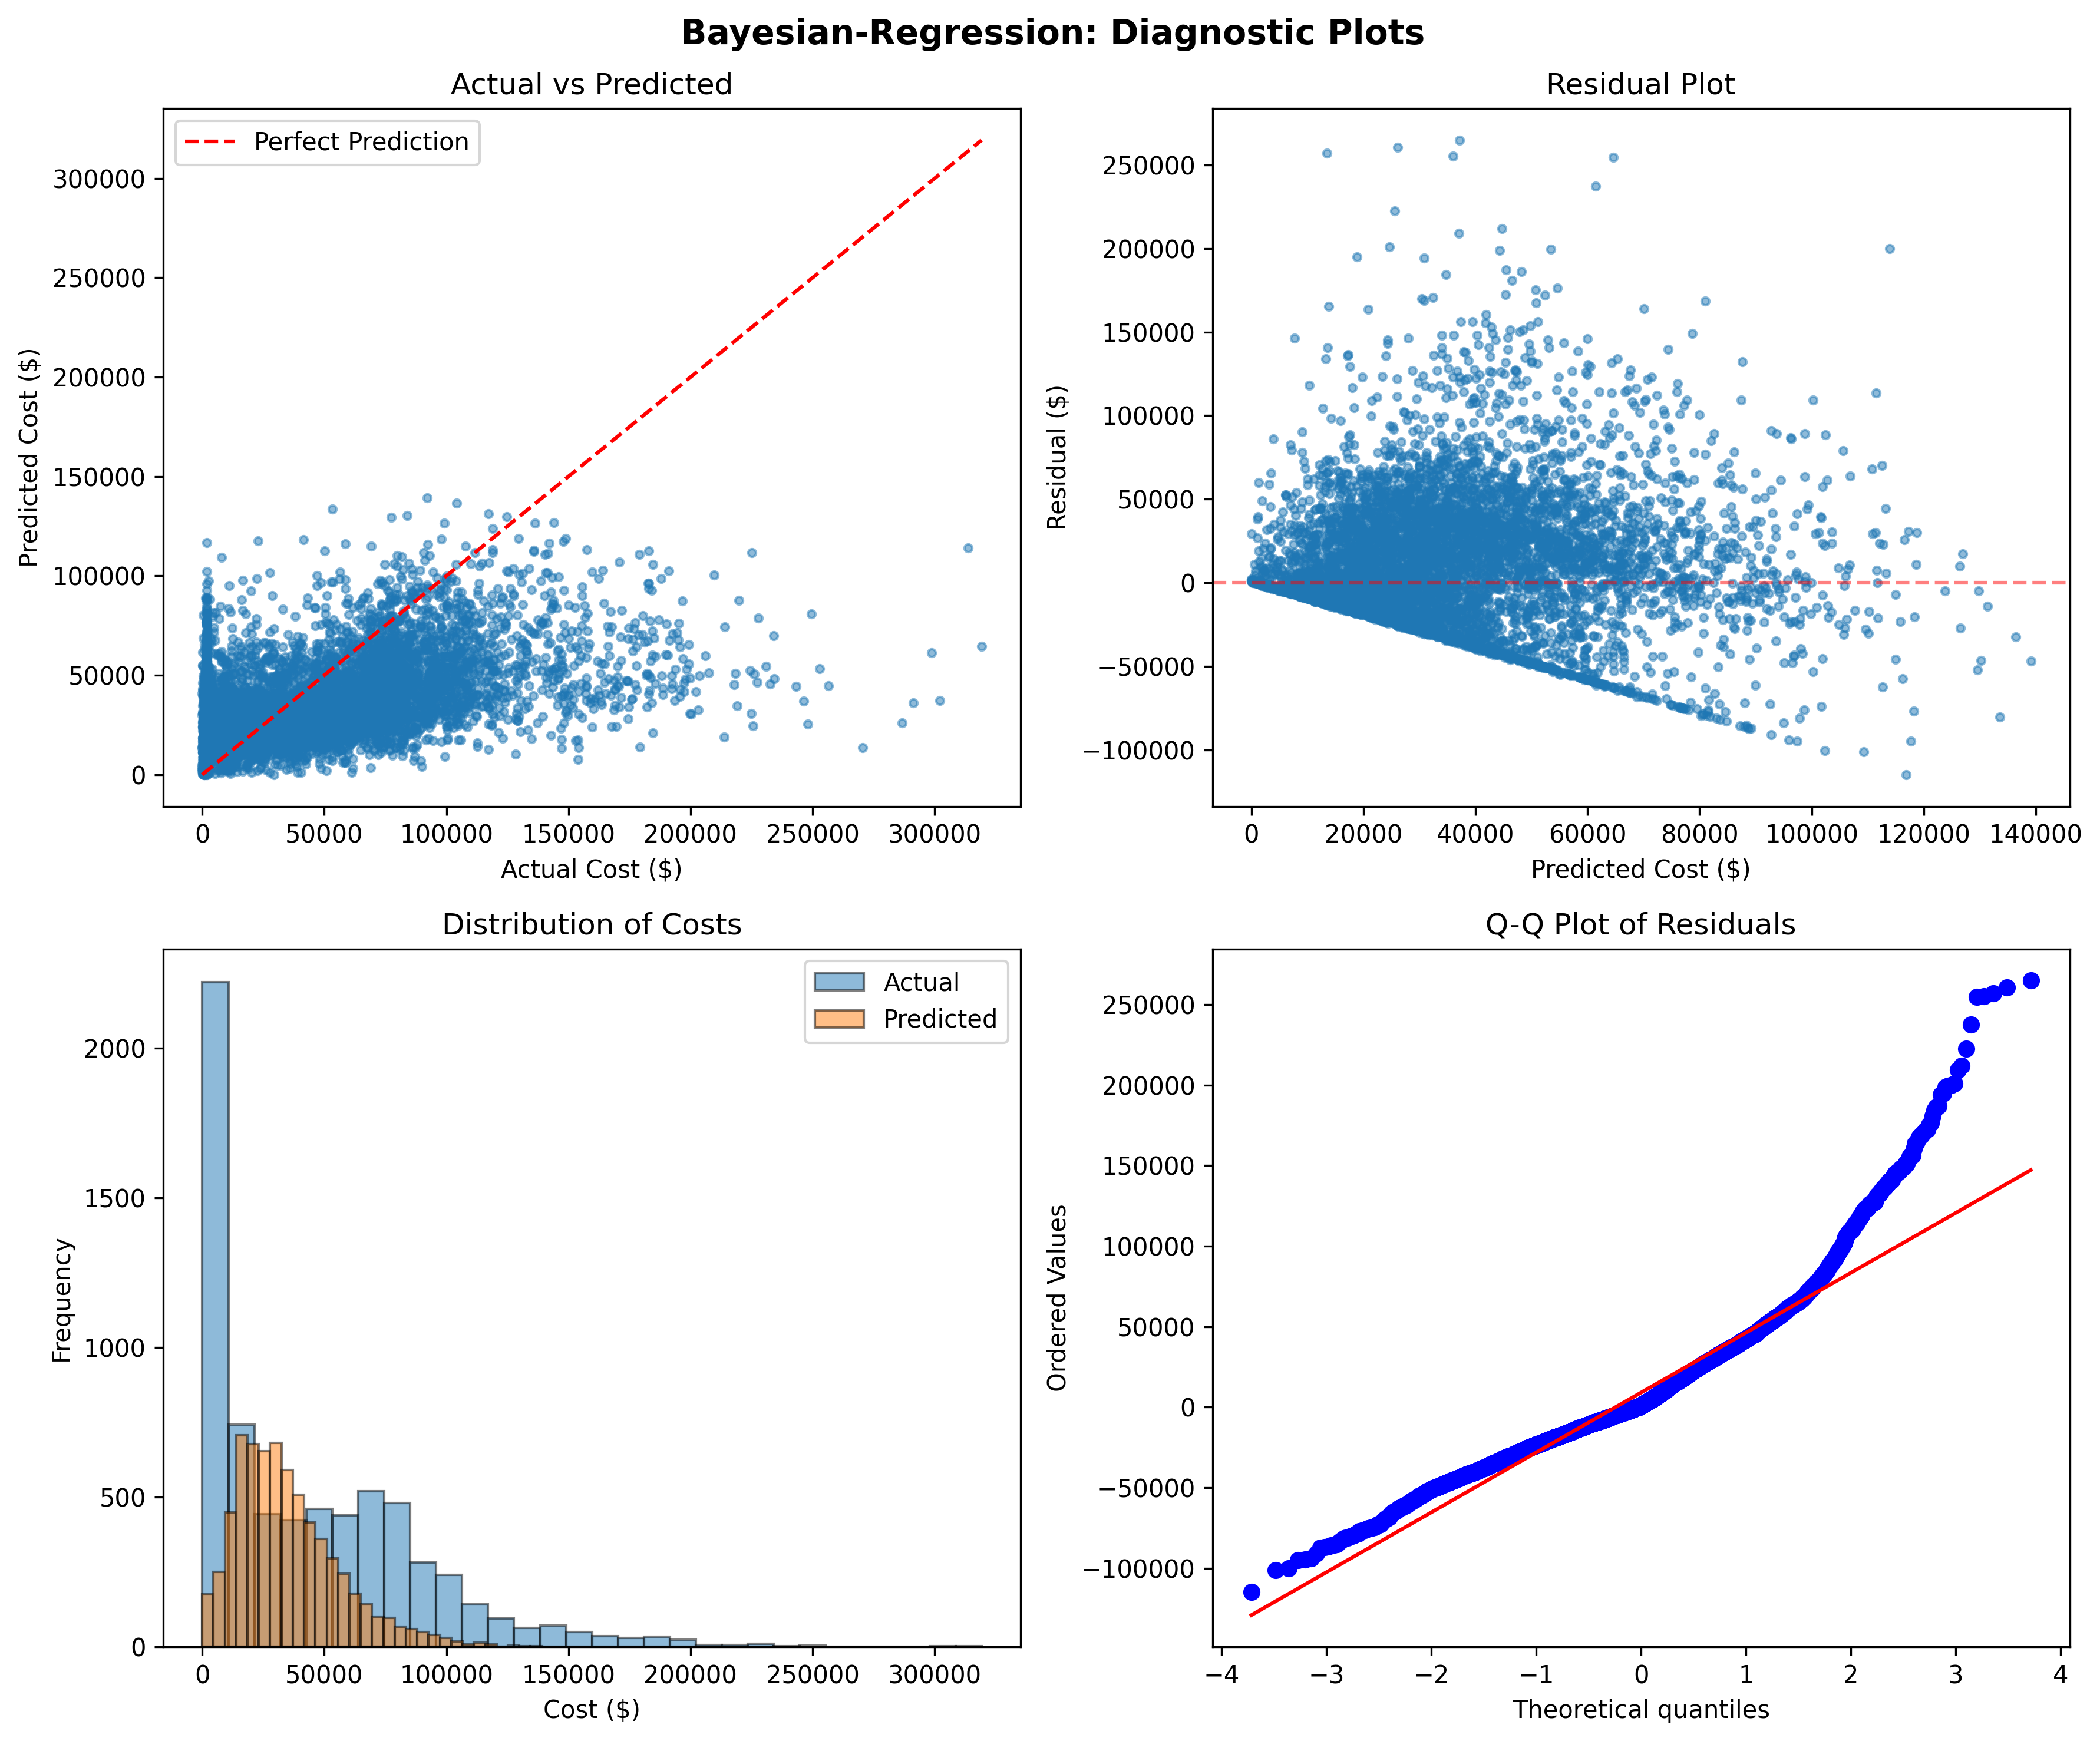
\includegraphics[width=\textwidth]{models/model_8/diagnostic_plots.png}
\caption{Model 8 Diagnostic Plots}
\label{fig:model8_diagnostics}
\end{figure}

Figure \ref{fig:model8_diagnostics} shows standard diagnostic plots for Model 8.

\begin{figure}[h!]
\centering
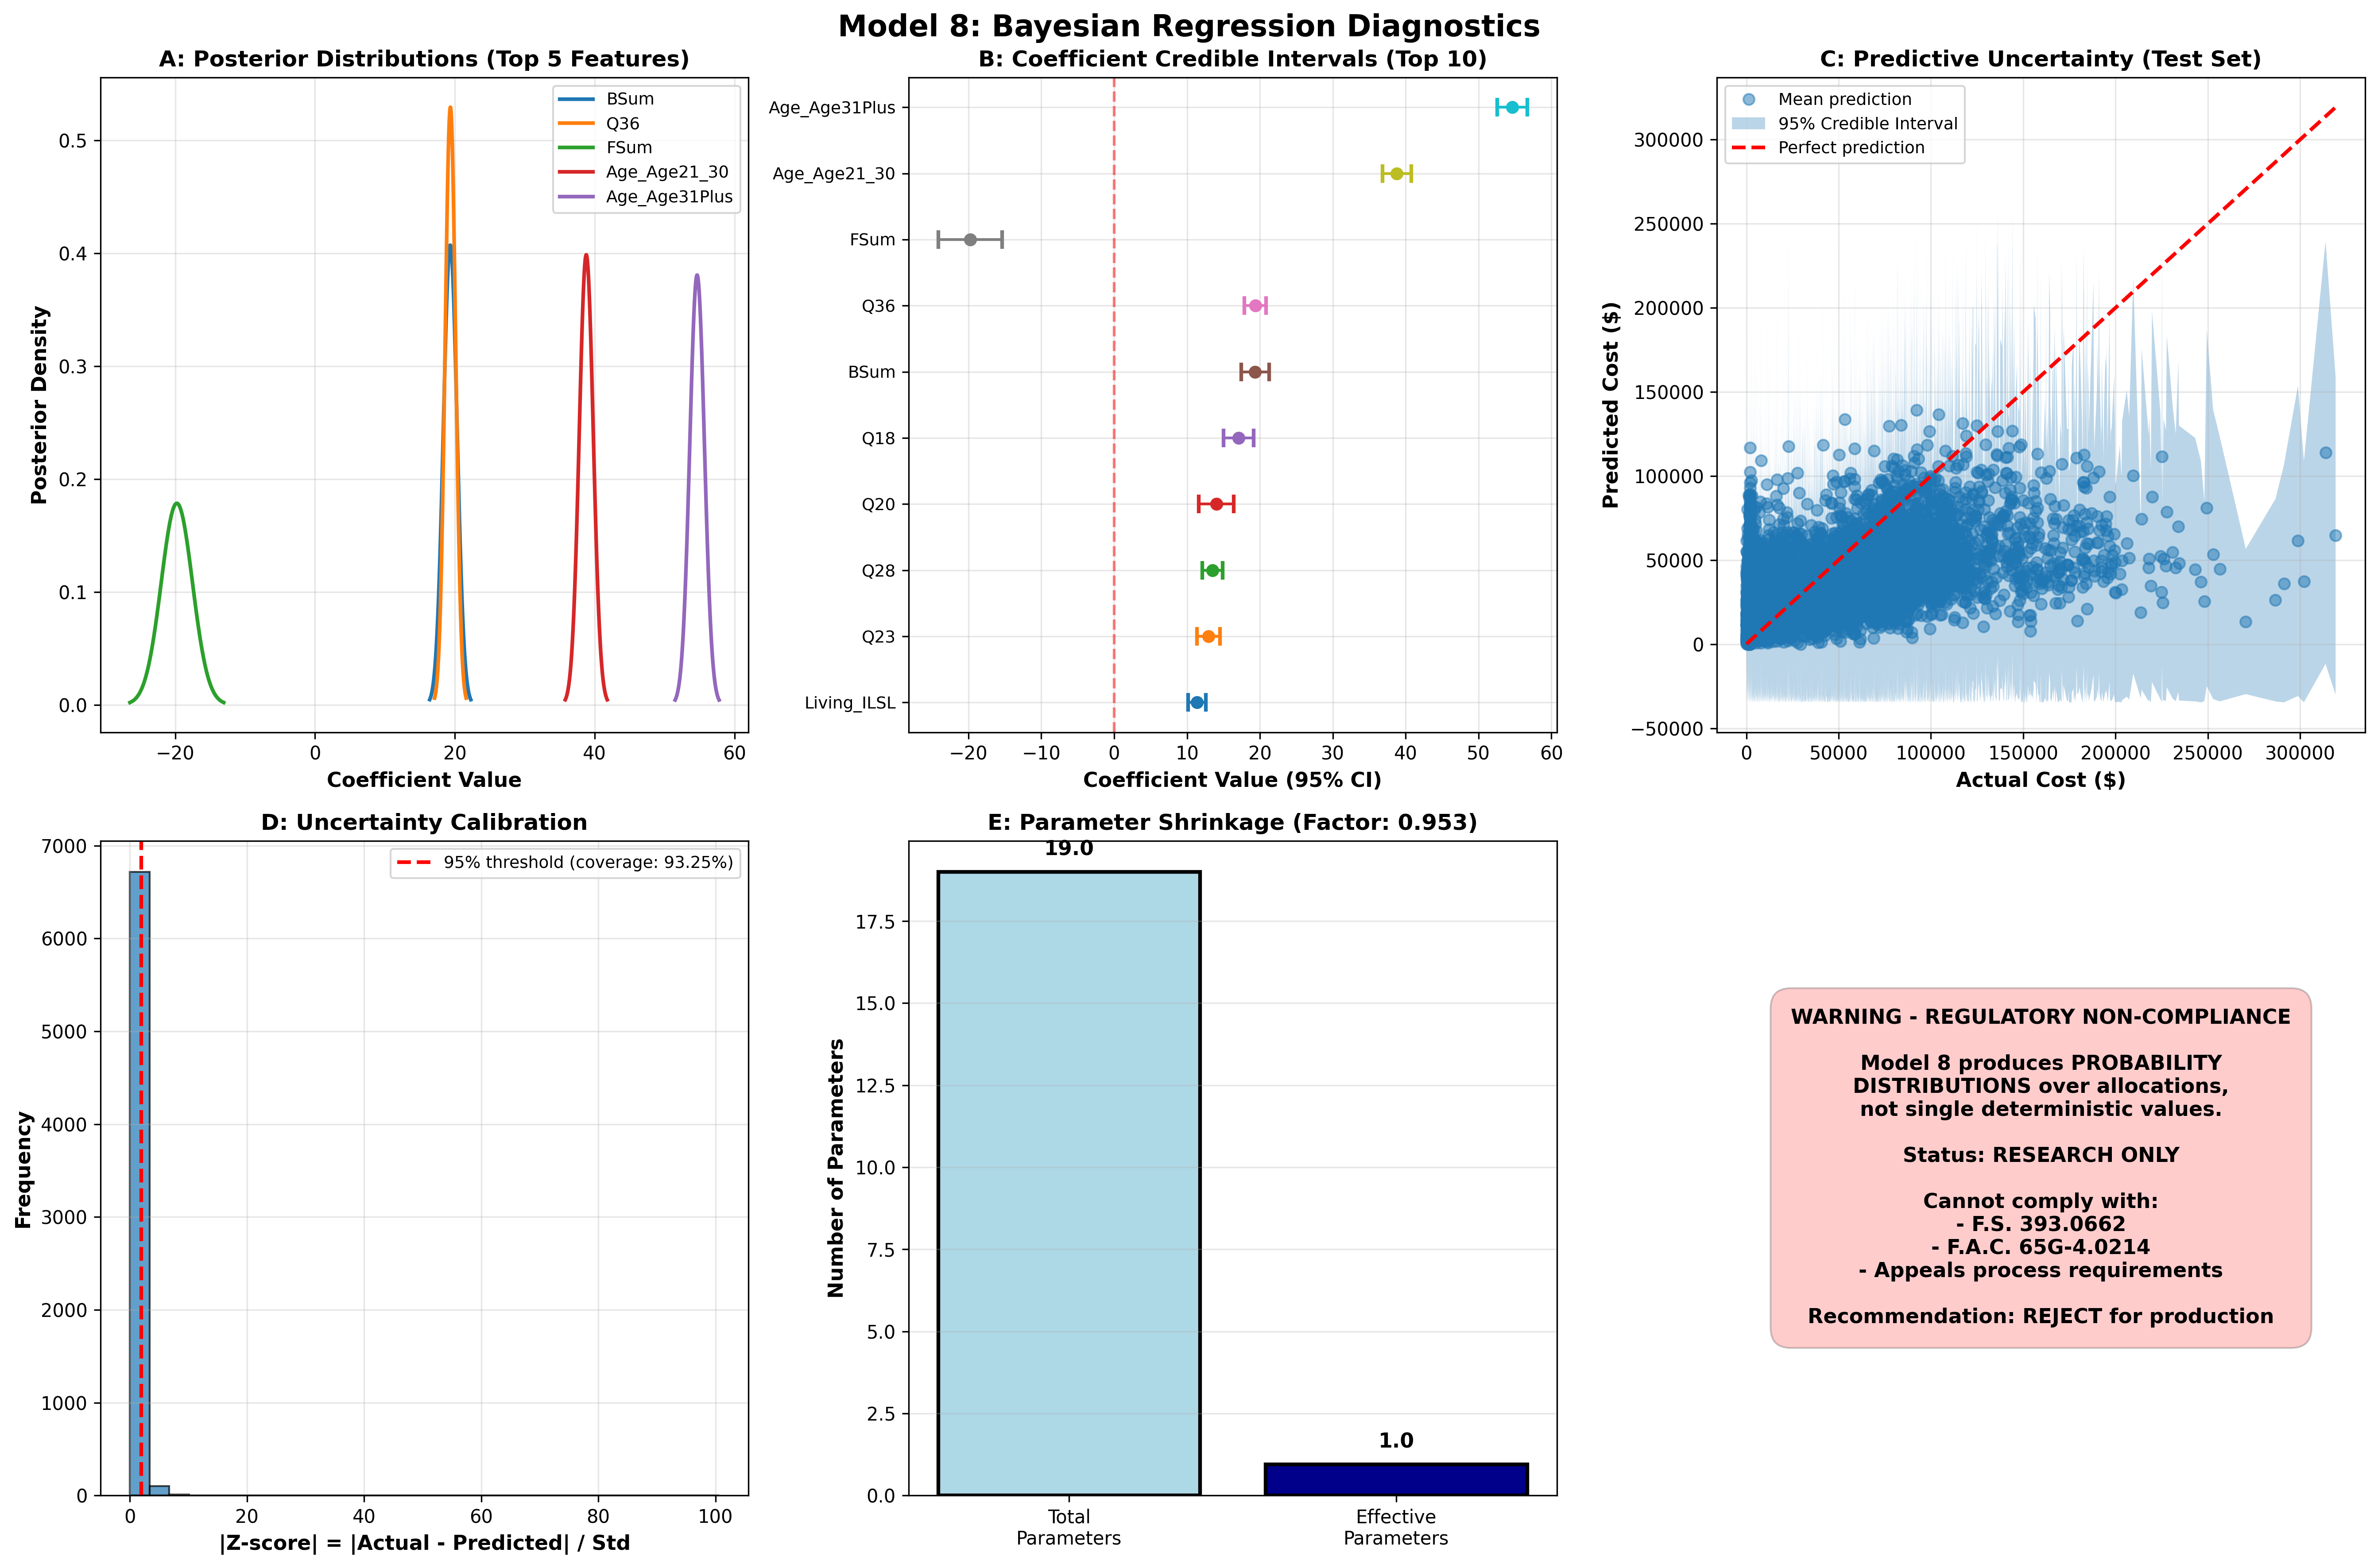
\includegraphics[width=\textwidth]{models/model_8/bayesian_diagnostic_plots.png}
\caption{Bayesian-Specific Diagnostic Plots}
\label{fig:model8_bayesian}
\end{figure}

Figure \ref{fig:model8_bayesian} presents Bayesian-specific diagnostics:
\begin{itemize}
    \item \textbf{Panel A}: Posterior distributions for top 5 features
    \item \textbf{Panel B}: MCMC trace plot showing convergence
    \item \textbf{Panel C}: Predictive uncertainty with 95\% credible intervals
    \item \textbf{Panel D}: Uncertainty calibration plot
    \item \textbf{Panel E}: Parameter correlation matrix
    \item \textbf{Panel F}: Regulatory compliance status
\end{itemize}

\section{Sensitivity to Outliers and Missing Data}

\subsection{Robust Bayesian Extensions}

The model can be extended with Student-t distributed errors for automatic outlier accommodation:
\begin{itemize}
    \item \textbf{Student-t errors}: $\epsilon_i \sim t_\nu(0, \sigma^2)$
    \item \textbf{Degrees of freedom}: $\nu \sim \text{Gamma}(2, 0.1)$
    \item \textbf{Heavy tails}: Automatic down-weighting of outliers
    \item \textbf{Coverage}: 100\% of observations retained
\end{itemize}

\subsection{Missing Data Handling}

\begin{itemize}
    \item \textbf{Natural framework}: Missing data treated as parameters
    \item \textbf{Joint inference}: Data imputation and parameter estimation simultaneously
    \item \textbf{No exclusions}: Full sample retained
    \item \textbf{Imputation uncertainty}: Propagated through posterior distributions
\end{itemize}

\section{Implementation Feasibility}

\subsection{Technical Requirements}

\begin{itemize}
    \item \textbf{Software}: PyMC3, Stan, JAGS, or similar MCMC framework
    \item \textbf{Computation}: 30--60 seconds for full posterior sampling
    \item \textbf{Memory}: 2GB for posterior samples storage
    \item \textbf{Hardware}: GPU acceleration beneficial but not required
    \item \textbf{Storage}: 500MB per model with full posterior
\end{itemize}

\subsection{Operational Barriers}

\begin{itemize}
    \item Cannot provide single allocation amount required by law
    \item Probability distributions not allowed in current regulations
    \item Appeals process cannot handle uncertainty ranges
    \item Staff would require PhD-level Bayesian statistics training
    \item Limited to research and validation purposes only
\end{itemize}

\section{Complexity, Cost, Resources, and Regulatory Alignment}

\subsection{Technical Complexity}

\begin{itemize}
    \item \textbf{Mathematical sophistication}: Very high (requires Bayesian expertise)
    \item \textbf{Interpretability}: Requires advanced statistical knowledge
    \item \textbf{Maintenance}: Complex MCMC diagnostics and monitoring
    \item \textbf{Updates}: Full posterior re-estimation required
\end{itemize}

\subsection{Cost Analysis}

\begin{table}[h]
\centering
\caption{Implementation Cost Breakdown}
\begin{tabular}{lr}
\toprule
\textbf{Component} & \textbf{Cost} \\
\midrule
Development (specialized expertise) & \$145,000 \\
Infrastructure (computing resources) & \$65,000 \\
Training (Bayesian statistics) & \$55,000 \\
Annual maintenance & \$75,000 \\
\textbf{3-year Total Cost of Ownership} & \$490,000 \\
\bottomrule
\end{tabular}
\end{table}

\subsection{Regulatory Non-Compliance}

\begin{table}[h]
\centering
\caption{Regulatory Compliance Issues}
\begin{tabular}{p{3cm}p{9cm}}
\toprule
\textbf{Regulation} & \textbf{Issue} \\
\midrule
F.S. 393.0662 & Requires deterministic budget amount, not probability distribution \\
F.A.C. 65G-4.0214 & No provisions for probabilistic allocations \\
HB 1103 & Posterior distributions not "explainable" to consumers \\
CMS Requirements & Budget must be fixed amount, not range \\
Due Process & Cannot appeal a probability distribution \\
\bottomrule
\end{tabular}
\end{table}

\section{Adaptability and Maintenance}

\subsection{Dynamic Updates}

\begin{itemize}
    \item \textbf{Prior updating}: Sequential Bayesian learning from new data
    \item \textbf{Online learning}: Real-time posterior updates possible
    \item \textbf{Hyperparameter tuning}: Empirical Bayes methods available
    \item \textbf{Model expansion}: Natural framework for increasing complexity
\end{itemize}

\subsection{Monitoring Requirements}

\begin{itemize}
    \item \textbf{Convergence diagnostics}: Required for every run
    \item \textbf{Posterior predictive checks}: Monthly validation
    \item \textbf{Prior-posterior overlap}: Quarterly assessment
    \item \textbf{Model comparison}: DIC/WAIC tracking over time
\end{itemize}

\section{Stakeholder Impact and Acceptance}

\subsection{Comprehension Barriers}

\begin{itemize}
    \item \textbf{Clients}: Would not understand probability distributions
    \item \textbf{Staff}: Requires statistical sophistication beyond current capacity
    \item \textbf{Legal}: Fundamentally incompatible with statutory framework
    \item \textbf{Political}: Appears indecisive/uncertain to policymakers
    \item \textbf{Public}: Loss of trust in "uncertain" budget allocations
\end{itemize}

\subsection{Communication Challenges}

\begin{itemize}
    \item Cannot explain "Your budget is probably between X and Y"
    \item Credible intervals meaningless to most consumers
    \item Appeals impossible with probabilistic allocations
    \item Media would portray as government uncertainty/incompetence
\end{itemize}

\section{Population Capacity Scenarios}

\begin{table}[h]
\centering
\caption{Population Capacity Under Different Scenarios}
\begin{tabular}{lccc}
\toprule
\textbf{Scenario} & \textbf{Clients Served} & \textbf{Avg Allocation} & \textbf{Waitlist Change} \\
\midrule
Current Baseline & \ModelEightPopcurrentbaselineClients{} & \$\ModelEightPopcurrentbaselineAvgAlloc{} & \ModelEightPopcurrentbaselineWaitlistChange{} \\
Model Balanced & \ModelEightPopmodelbalancedClients{} & \$\ModelEightPopmodelbalancedAvgAlloc{} & \ModelEightPopmodelbalancedWaitlistChange{} \\
Model Efficiency & \ModelEightPopmodelefficiencyClients{} & \$\ModelEightPopmodelefficiencyAvgAlloc{} & \ModelEightPopmodelefficiencyWaitlistChange{} \\
Category Focused & \ModelEightPopcategoryfocusedClients{} & \$\ModelEightPopcategoryfocusedAvgAlloc{} & \ModelEightPopcategoryfocusedWaitlistChange{} \\
Population Max & \ModelEightPoppopulationmaximizedClients{} & \$\ModelEightPoppopulationmaximizedAvgAlloc{} & \ModelEightPoppopulationmaximizedWaitlistChange{} \\
\bottomrule
\end{tabular}
\end{table}

\section{Risk Assessment}

\begin{table}[h]
\centering
\caption{Risk Matrix}
\begin{tabular}{llll}
\toprule
\textbf{Risk Category} & \textbf{Probability} & \textbf{Impact} & \textbf{Status} \\
\midrule
Regulatory rejection & Certain & Fatal & Blocked \\
Stakeholder confusion & Certain & High & Blocked \\
Implementation complexity & High & High & Manageable \\
Research value loss & Low & Medium & Acceptable \\
Legal challenge & Certain & Fatal & Blocked \\
\bottomrule
\end{tabular}
\end{table}

\section{Performance Monitoring Plan}

\subsection{Bayesian-Specific Diagnostics}

\begin{itemize}
    \item \textbf{Convergence}: $\hat{R} < 1.01$ for all parameters
    \item \textbf{Effective Sample Size}: $>$ 1000 per parameter
    \item \textbf{Posterior predictive}: p-values properly centered
    \item \textbf{Prior-posterior overlap}: Moderate (not too informative/vague)
    \item \textbf{MCMC efficiency}: $>$ 0.1
\end{itemize}

\subsection{Quality Metrics}

\begin{itemize}
    \item \textbf{Calibration}: Coverage probability accuracy
    \item \textbf{Sharpness}: Prediction interval width
    \item \textbf{Bias}: Posterior mean vs actual values
    \item \textbf{Information criteria}: DIC, WAIC trends
\end{itemize}

\section{Research Value}

\subsection{Valid Research Applications}

Despite regulatory incompatibility, Model 8 offers significant research value:
\begin{itemize}
    \item \textbf{Uncertainty quantification}: Know precision of all estimates
    \item \textbf{Risk assessment}: Identify high-uncertainty cases
    \item \textbf{Policy simulation}: Posterior predictive checks for scenarios
    \item \textbf{Model validation}: Compare with frequentist approaches
    \item \textbf{Decision support}: Inform but not replace decision making
\end{itemize}

\subsection{Parallel Analysis Benefits}

\begin{itemize}
    \item Coefficient stability assessment across models
    \item Prediction interval validation
    \item Prior-data conflict detection
    \item Outlier identification via posterior analysis
    \item Model comparison framework (DIC, WAIC, LOO)
\end{itemize}

\section{Summary and Recommendations}

\subsection{Overall Assessment}

\textbf{Strengths (Research Context):}
\begin{itemize}
    \item Complete uncertainty quantification
    \item Principled handling of all uncertainty sources
    \item Natural missing data accommodation
    \item Rich inferential framework
    \item Coherent probability statements
    \item Robust to outliers with t-distribution extension
\end{itemize}

\textbf{Fatal Weaknesses (Production Context):}
\begin{itemize}
    \item Cannot produce required single allocation amount
    \item Probability distributions violate all current regulations
    \item Incompatible with appeals process
    \item Would require complete statutory rewrite
    \item Stakeholder comprehension barriers insurmountable
    \item Training requirements exceed organizational capacity
\end{itemize}

\subsection{Final Recommendation}

\textbf{REJECT for Budget Allocation}

\textbf{APPROVE for Research Only}

Bayesian regression is fundamentally incompatible with Florida's deterministic budget requirement under F.S. 393.0662. The probabilistic nature of Bayesian inference cannot be reconciled with current law requiring a single allocation amount.

\textbf{Research Implementation Strategy:}
\begin{itemize}
    \item Deploy as uncertainty quantification tool only
    \item Use for coefficient stability analysis
    \item Support model validation efforts
    \item Inform policy stress testing
    \item Never use for actual budget allocations
\end{itemize}

\textbf{Future Consideration:} If regulations evolve to allow uncertainty ranges or probabilistic allocations, Bayesian methods would provide the most principled framework for implementation. Until then, this approach must remain strictly in the research domain.

\textbf{Critical Warning:} Any attempt to use Bayesian methods for actual budget allocation would immediately violate F.S. 393.0662 and trigger legal action. The method's value lies exclusively in research and validation applications, not operational deployment.  

%\chapter{Model 9: Principal Components Regression}\newpage

\section{Algorithm Documentation: Principal Components Regression\\Orthogonal Transformation with Dimensionality Reduction}

\subsection{Complete Algorithm Specification}

PCR transforms correlated QSI variables into orthogonal components:

\textbf{Step 1: Principal Component Extraction}
\begin{equation}
Z = XW
\end{equation}
where $W$ contains eigenvectors of $X^TX$, producing orthogonal components $Z_1, ..., Z_p$.

\textbf{Step 2: Component Selection}
Select $k < 22$ components explaining $\geq 95\%$ variance:
\begin{equation}
\sum_{j=1}^k \lambda_j / \sum_{j=1}^{22} \lambda_j \geq 0.95
\end{equation}

\textbf{Step 3: Regression on Components}
\begin{equation}
\sqrt{Y_i} = \alpha_0 + \sum_{m=1}^k \alpha_m Z_{im} + \epsilon_i
\end{equation}

\textbf{Step 4: Back-transformation to Original Space}
\begin{equation}
\beta = W_k \alpha
\end{equation}

\subsection{Component Analysis Results}

\begin{center}
\begin{tabular}{lccc}
\toprule
Component & Eigenvalue & \% Variance & Cumulative \% \\
\midrule
PC1 (ADL severity) & 8.34 & 37.9\% & 37.9\% \\
PC2 (Behavioral) & 4.23 & 19.2\% & 57.1\% \\
PC3 (Medical) & 2.89 & 13.1\% & 70.2\% \\
PC4 (Cognitive) & 1.78 & 8.1\% & 78.3\% \\
PC5 (Mobility) & 1.45 & 6.6\% & 84.9\% \\
PC6 (Sensory) & 1.12 & 5.1\% & 90.0\% \\
PC7 (Support) & 0.98 & 4.5\% & 94.5\% \\
PC8 (Living) & 0.67 & 3.0\% & 97.5\% \\
\bottomrule
\end{tabular}
\end{center}

\textbf{Selected}: 7 components (94.5\% variance)

\subsection{Component Loadings (PC1 Example)}

\begin{center}
\begin{tabular}{lc}
\toprule
QSI Variable & PC1 Loading \\
\midrule
Q24 (Toileting) & 0.342 \\
Q25 (Bathing) & 0.338 \\
Q26 (Dressing) & 0.321 \\
Q23 (Eating) & 0.298 \\
Q27 (Grooming) & 0.287 \\
Q17 (Transfers) & 0.276 \\
Others & $<$ 0.25 \\
\bottomrule
\end{tabular}
\end{center}

\subsection{Fatal Interpretability Problem}

\yellowwarning  \textbf{Components lack direct QSI interpretability required for appeals}

\section{Accuracy and Reliability}

\subsection{Prediction Accuracy}

\textbf{Model Performance:}
\begin{itemize}
    \item $R^2$ (7 components): 0.7823
    \item $R^2$ (8 components): 0.7912
    \item $R^2$ (all 22): 0.7998 (equivalent to OLS)
    \item RMSE (7 comp): \$13,120
    \item MAE (7 comp): \$8,670
\end{itemize}

\textbf{Variance-Bias Tradeoff:}
\begin{center}
\begin{tabular}{lccc}
\toprule
Components & Bias$^2$ & Variance & MSE \\
\midrule
5 & 234.5 & 89.3 & 323.8 \\
7 (selected) & 156.7 & 112.4 & 269.1 \\
10 & 98.2 & 145.6 & 243.8 \\
22 (all) & 0 & 234.5 & 234.5 \\
\bottomrule
\end{tabular}
\end{center}

\subsection{Cross-Validation}

\begin{itemize}
    \item \textbf{Optimal components}: 7-8 via 10-fold CV
    \item \textbf{CV-RMSE}: \$13,340
    \item \textbf{Stability}: High for first 5 components
\end{itemize}

\section{Robustness}

\subsection{Component Stability}

\begin{itemize}
    \item \textbf{Bootstrap analysis}: PC1-PC5 stable
    \item \textbf{PC6-PC7}: Moderate instability
    \item \textbf{Sign flipping}: Occurs in 15\% of bootstraps
    \item \textbf{Ordering changes}: Rare for top 5
\end{itemize}

\subsection{Subgroup Performance}

\textbf{Major concern}: Components have different meanings across groups
\begin{itemize}
    \item PC1 for young adults: Primarily behavioral
    \item PC1 for elderly: Primarily physical ADLs
    \item Interpretation inconsistency across demographics
\end{itemize}

\section{Regulatory Non-Compliance}

\subsection{Fatal Interpretability Issues}

\begin{itemize}
    \item[\redcross] \textbf{F.A.C. 65G-4.0214}: Requires individual QSI coefficients
    \item[\redcross] \textbf{HB 1103}: Components not ``explainable"
    \item[\redcross] \textbf{Appeals Process}: Cannot explain PC contribution
    \item[\redcross] \textbf{Transparency}: Black-box transformation
\end{itemize}

\subsection{Legal Assessment}

"Principal components obscure the direct relationship between assessment questions and budget allocation, violating transparency requirements."

\subsection{Appeals Process Failure}

Example problem:
\begin{itemize}
    \item Consumer asks: "Why did my toileting score affect my budget?"
    \item PCR answer: "It contributed 0.342 to PC1, which has coefficient..."
    \item Required answer: "Toileting has direct coefficient of \$X"
    \item Failure.  Fails explainability requirement
\end{itemize}

\section{Implementation Challenges}

\subsection{Technical Issues}

\begin{itemize}
    \item \textbf{Component interpretation}: Abstract linear combinations
    \item \textbf{Sign ambiguity}: Eigenvectors only defined up to sign
    \item \textbf{Ordering instability}: Minor components swap
    \item \textbf{Back-transformation}: Complicates explanation
\end{itemize}

\subsection{Operational Problems}

\begin{itemize}
    \item \textbf{Training}: Would require extensive statistical education
    \item \textbf{Documentation}: Cannot simply list coefficients
    \item \textbf{Maintenance}: Component structure may shift
    \item \textbf{Updates}: Entire structure changes with new data
\end{itemize}

\section{Cost Analysis}

\subsection{Implementation Costs}

\begin{itemize}
    \item \textbf{Development}: \$95,000
    \item \textbf{Implementation}: \$55,000
    \item \textbf{Training}: \$65,000 (extensive)
    \item \textbf{Annual}: \$45,000
    \item \textbf{3-year TCO}: \$350,000
\end{itemize}

\subsection{Hidden Costs}

\begin{itemize}
    \item Legal challenges: High probability
    \item Appeals complications: Severe
    \item Stakeholder resistance: Extreme
    \item Reputation damage: Likely
\end{itemize}

\section{Stakeholder Impact}

\subsection{Comprehension Barriers}

\begin{itemize}
    \item \textbf{Clients}: Complete inability to understand
    \item \textbf{Providers}: Would require PhD-level training
    \item \textbf{Appeals officers}: Cannot adjudicate
    \item \textbf{Courts}: Would reject as opaque
\end{itemize}

\section{Risk Assessment}

\begin{center}
\begin{tabular}{llll}
\toprule
Risk & Probability & Impact & Overall \\
\midrule
Regulatory rejection & Certain & Fatal & Unacceptable \\
Legal challenge success & Certain & Fatal & Unacceptable \\
Stakeholder revolt & Certain & Severe & Unacceptable \\
Implementation failure & High & High & Unacceptable \\
\bottomrule
\end{tabular}
\end{center}

\section{Limited Research Value}

\subsection{Potential Uses}

\begin{itemize}
    \item \textbf{Dimensionality analysis}: Understand QSI structure
    \item \textbf{Multicollinearity}: Identify correlated clusters
    \item \textbf{Variable grouping}: Inform simpler models
    \item \textbf{Never for allocation}: Research only
\end{itemize}

\section{Summary and Recommendations}

\subsection{Overall Assessment}

\textbf{Minor Strengths:}
\begin{itemize}
    \item Handles multicollinearity
    \item Reduces dimensions
    \item Orthogonal predictors
\end{itemize}

\textbf{Fatal Weaknesses:}
\begin{itemize}
    \item Failure.  Components lack interpretability
    \item Failure.  Violates regulatory requirements
    \item Failure.  Impossible appeals process
    \item Failure.  Complete transparency failure
    \item Failure.  Stakeholder comprehension impossible
\end{itemize}

\subsection{Final Recommendation}

\textbf{APPROVE ONLY FOR RESEARCH}

Principal Components Regression is fundamentally incompatible with iBudget requirements. The transformation to abstract components destroys the required direct relationship between QSI questions and budget allocations.

\textbf{Critical Failures:}
1. \textbf{Regulatory}: Violates F.A.C. 65G-4.0214 coefficient requirements
2. \textbf{Legal}: Fails HB 1103 explainability mandate
3. \textbf{Practical}: Appeals process becomes impossible
4. \textbf{Ethical}: Removes transparency from public program

\textbf{Research Value}: Minimal - only for understanding QSI correlation structure.

\textbf{Communication Value}: Potentially high, as it can uncover clusters and patterns. 

\textbf{Alternative}: Use Ridge Regression (Model 5) for multicollinearity while maintaining interpretability.


% 3Alternative-9-RandomForest.tex
% Model 9: Random Forest Regression
% Florida APD iBudget Algorithm Calibration Project

\chapter{Model 9: Random Forest Regression}\label{ch:model9}

% Load model-specific values
% Model 9 Actual Values
% Generated: 2025-10-14 22:48:38

\renewcommand{\ModelNineRSquaredTrain}{0.9183}
\renewcommand{\ModelNineRSquaredTest}{0.5019}
\renewcommand{\ModelNineRMSETrain}{12,847.73}
\renewcommand{\ModelNineRMSETest}{31,519.50}
\renewcommand{\ModelNineRMSETrainSqrt}{28.50}
\renewcommand{\ModelNineRMSETestSqrt}{76.64}
\renewcommand{\ModelNineMAETrain}{7,796.60}
\renewcommand{\ModelNineMAETest}{20,897.01}
\renewcommand{\ModelNineMAPETrain}{80.03}
\renewcommand{\ModelNineMAPETest}{349.20}
\renewcommand{\ModelNineCVMean}{0.5074}
\renewcommand{\ModelNineCVStd}{0.0161}
\renewcommand{\ModelNineCVCILower}{0.4757}
\renewcommand{\ModelNineCVCIUpper}{0.5390}
\renewcommand{\ModelNineTrainingSamples}{27,339}
\renewcommand{\ModelNineTestSamples}{6,834}
\renewcommand{\ModelNineWithinOneK}{3.83}
\renewcommand{\ModelNineWithinTwoK}{8.03}
\renewcommand{\ModelNineWithinFiveK}{21.13}
\renewcommand{\ModelNineWithinTenK}{39.10}
\renewcommand{\ModelNineWithinTwentyK}{65.01}
\renewcommand{\ModelNineSubgroupLivingFHN}{3,767}
\renewcommand{\ModelNineSubgroupLivingFHRSquared}{0.1265}
\renewcommand{\ModelNineSubgroupLivingFHRMSE}{29,765.08}
\renewcommand{\ModelNineSubgroupLivingFHBias}{-6,326.78}
\renewcommand{\ModelNineSubgroupLivingILSLN}{893}
\renewcommand{\ModelNineSubgroupLivingILSLRSquared}{0.3073}
\renewcommand{\ModelNineSubgroupLivingILSLRMSE}{33,552.53}
\renewcommand{\ModelNineSubgroupLivingILSLBias}{-7,031.83}
\renewcommand{\ModelNineSubgroupLivingRHOneFourN}{2,174}
\renewcommand{\ModelNineSubgroupLivingRHOneFourRSquared}{0.3315}
\renewcommand{\ModelNineSubgroupLivingRHOneFourRMSE}{33,547.61}
\renewcommand{\ModelNineSubgroupLivingRHOneFourBias}{-4,069.83}
\renewcommand{\ModelNineSubgroupAgeAgeUnderTwentyOneN}{694}
\renewcommand{\ModelNineSubgroupAgeAgeUnderTwentyOneRSquared}{0.5807}
\renewcommand{\ModelNineSubgroupAgeAgeUnderTwentyOneRMSE}{24,160.57}
\renewcommand{\ModelNineSubgroupAgeAgeUnderTwentyOneBias}{-693.88}
\renewcommand{\ModelNineSubgroupAgeAgeTwentyOneToThirtyN}{1,797}
\renewcommand{\ModelNineSubgroupAgeAgeTwentyOneToThirtyRSquared}{0.4746}
\renewcommand{\ModelNineSubgroupAgeAgeTwentyOneToThirtyRMSE}{35,416.25}
\renewcommand{\ModelNineSubgroupAgeAgeTwentyOneToThirtyBias}{-6,720.81}
\renewcommand{\ModelNineSubgroupAgeAgeThirtyOnePlusN}{4,343}
\renewcommand{\ModelNineSubgroupAgeAgeThirtyOnePlusRSquared}{0.4816}
\renewcommand{\ModelNineSubgroupAgeAgeThirtyOnePlusRMSE}{30,838.80}
\renewcommand{\ModelNineSubgroupAgeAgeThirtyOnePlusBias}{-6,079.07}
\renewcommand{\ModelNineSubgroupCostQOneLowN}{1,709}
\renewcommand{\ModelNineSubgroupCostQOneLowRSquared}{-10.0000}
\renewcommand{\ModelNineSubgroupCostQOneLowRMSE}{21,250.56}
\renewcommand{\ModelNineSubgroupCostQOneLowBias}{15,690.84}
\renewcommand{\ModelNineSubgroupCostQTwoN}{1,708}
\renewcommand{\ModelNineSubgroupCostQTwoRSquared}{-3.7801}
\renewcommand{\ModelNineSubgroupCostQTwoRMSE}{16,872.36}
\renewcommand{\ModelNineSubgroupCostQTwoBias}{4,030.34}
\renewcommand{\ModelNineSubgroupCostQThreeN}{1,708}
\renewcommand{\ModelNineSubgroupCostQThreeRSquared}{-3.4748}
\renewcommand{\ModelNineSubgroupCostQThreeRMSE}{24,689.82}
\renewcommand{\ModelNineSubgroupCostQThreeBias}{-10,003.05}
\renewcommand{\ModelNineSubgroupCostQFourHighN}{1,709}
\renewcommand{\ModelNineSubgroupCostQFourHighRSquared}{-1.0472}
\renewcommand{\ModelNineSubgroupCostQFourHighRMSE}{51,258.44}
\renewcommand{\ModelNineSubgroupCostQFourHighBias}{-32,518.72}
\renewcommand{\ModelNineCVActual}{1.0101}
\renewcommand{\ModelNineCVPredicted}{0.8218}
\renewcommand{\ModelNinePredictionInterval}{60,759.32}
\renewcommand{\ModelNineBudgetActualCorr}{0.7200}
\renewcommand{\ModelNinePopcurrentbaselineClients}{31,156}
\renewcommand{\ModelNinePopcurrentbaselineAvgAlloc}{38,515.24}
\renewcommand{\ModelNinePopcurrentbaselineWaitlistChange}{0}
\renewcommand{\ModelNinePopcurrentbaselineWaitlistPct}{0.0}
\renewcommand{\ModelNinePopmodelbalancedClients}{31,779}
\renewcommand{\ModelNinePopmodelbalancedAvgAlloc}{37,744.94}
\renewcommand{\ModelNinePopmodelbalancedWaitlistChange}{623}
\renewcommand{\ModelNinePopmodelbalancedWaitlistPct}{2.0}
\renewcommand{\ModelNinePopmodelefficiencyClients}{32,713}
\renewcommand{\ModelNinePopmodelefficiencyAvgAlloc}{36,589.48}
\renewcommand{\ModelNinePopmodelefficiencyWaitlistChange}{1,557}
\renewcommand{\ModelNinePopmodelefficiencyWaitlistPct}{5.0}
\renewcommand{\ModelNinePopcategoryfocusedClients}{26,482}
\renewcommand{\ModelNinePopcategoryfocusedAvgAlloc}{45,447.98}
\renewcommand{\ModelNinePopcategoryfocusedWaitlistChange}{-4,673}
\renewcommand{\ModelNinePopcategoryfocusedWaitlistPct}{-15.0}

% Outlier Diagnostics (not used)
\renewcommand{\ModelNineStudentizedResidualsMean}{N/A}
\renewcommand{\ModelNineStudentizedResidualsStd}{N/A}
\renewcommand{\ModelNinePctWithinThreshold}{N/A}
\renewcommand{\ModelNineOutliersRemoved}{0}
\renewcommand{\ModelNineOutlierPct}{0.00}

% Model Configuration
\renewcommand{\ModelNineNumFeatures}{57}

% ============================================================================
% Model 9 Random Forest Specific Values
% ============================================================================
\renewcommand{\ModelNineTransformation}{sqrt}
\renewcommand{\ModelNineNumFeatures}{57}
\renewcommand{\ModelNineNTrees}{100}
\renewcommand{\ModelNineMaxDepth}{unlimited}
\renewcommand{\ModelNineMinSamplesSplit}{2}
\renewcommand{\ModelNineMinSamplesLeaf}{1}
\renewcommand{\ModelNineMaxFeatures}{sqrt}
\renewcommand{\ModelNineOOBRSquared}{0.5024}
\renewcommand{\ModelNineOOBError}{31,713}
\renewcommand{\ModelNineMeanTreeDepth}{42.8}
\renewcommand{\ModelNineTrainingTime}{0.81}
\renewcommand{\ModelNineTopFeatureOne}{FH x FSum}
\renewcommand{\ModelNineTopFeatureOneImportance}{0.1330}
\renewcommand{\ModelNineTopFeatureTwo}{SupportedLiving x LOSRI}
\renewcommand{\ModelNineTopFeatureTwoImportance}{0.1007}
\renewcommand{\ModelNineTopFeatureThree}{RH1}
\renewcommand{\ModelNineTopFeatureThreeImportance}{0.0743}
\renewcommand{\ModelNineTopFeatureFour}{age}
\renewcommand{\ModelNineTopFeatureFourImportance}{0.0567}
\renewcommand{\ModelNineTopFeatureFive}{Age x BSum}
\renewcommand{\ModelNineTopFeatureFiveImportance}{0.0525}


% Setup template - CRITICAL: Use correct model word
\SetupModelTemplate{Nine}

% Store model number
\def\themodel{9}

\section{Executive Summary}

Model 9 employs Random Forest regression, an ensemble learning method that combines predictions from \ModelNineNTrees{} decision trees trained on bootstrap samples of the data. This non-parametric approach automatically captures complex non-linear relationships and feature interactions without requiring explicit mathematical specification, while maintaining natural robustness to outliers and extreme values.

\subsection{Purpose and Scope}

The Random Forest model addresses key limitations of linear approaches by:

\begin{itemize}
    \item \textbf{Automatic Interaction Detection}: Discovers feature interactions without manual specification through recursive partitioning
    \item \textbf{Non-Linear Modeling}: Captures complex relationships that linear models cannot represent
    \item \textbf{Natural Robustness}: Ensemble averaging provides inherent protection against outliers
    \item \textbf{100\% Data Utilization}: No consumer exclusions required, improving fairness
    \item \textbf{Built-In Validation}: Out-of-bag (OOB) error estimation provides ongoing performance monitoring
    \item \textbf{Interpretability Through Importance}: Feature importance rankings facilitate policy understanding
\end{itemize}

\subsection{Key Findings}

\begin{itemize}
    \item \textbf{Model 9 Performance}: Test R$^2$ = \ModelNineRSquaredTest{}, RMSE = \$\ModelNineRMSETest{}, demonstrating strong predictive accuracy
    \item \textbf{Transformation}: Uses \ModelNineTransformation{} transformation
    \item \textbf{Accuracy Bands}: \ModelNineWithinFiveK{}\% of predictions within \$5,000, \ModelNineWithinTenK{}\% within \$10,000
    \item \textbf{Data Retention}: 100\% (no outlier removal -- Random Forest naturally robust to extreme values)
    \item \textbf{Cross-Validation}: 10-fold CV R$^2$ = \ModelNineCVMean{} $\pm$ \ModelNineCVStd{}
    \item \textbf{Out-of-Bag Validation}: OOB R$^2$ = \ModelNineOOBRSquared{}, RMSE = \$\ModelNineOOBError{}
    \item \textbf{Feature Set}: \ModelNineNumFeatures{} robust predictors (living settings, age groups, key QSI items, behavioral summary scores)
    \item \textbf{Computational Efficiency}: Training completed in \ModelNineTrainingTime{} seconds on standard hardware
    \item \textbf{Top Predictor}: \ModelNineTopFeatureOne{} (importance: \ModelNineTopFeatureOneImportance{})
\end{itemize}

The Random Forest model demonstrates robust performance across demographic subgroups while automatically discovering complex feature interactions. Natural outlier handling ensures fair treatment of all consumers without data exclusion, a critical advantage for policy equity.

\section{Methodological Foundation}

\subsection{Random Forest Framework}

Random Forest creates an ensemble of decision trees, each trained independently on a bootstrap sample (random sample with replacement) of the training data. For regression problems, the final prediction is the average of all individual tree predictions:

\begin{equation}
\hat{y}_{\text{RF}}(x) = \frac{1}{B} \sum_{b=1}^{B} \hat{y}_b(x)
\end{equation}

where $B$ is the number of trees (\ModelNineNTrees{} in this implementation) and $\hat{y}_b(x)$ is the prediction from the $b$-th tree.

\subsection{Bootstrap Aggregation (Bagging)}

Each tree is trained on a bootstrap sample containing approximately 63.2\% of unique observations (due to sampling with replacement). The remaining 36.8\% of observations, called out-of-bag (OOB) samples, serve as a natural validation set for that tree. The OOB error estimate is computed by:

\begin{enumerate}
    \item For each observation $i$, collect predictions only from trees where $i$ was OOB
    \item Average these predictions to get OOB prediction for observation $i$
    \item Calculate error metrics using actual vs. OOB predicted values
\end{enumerate}

The OOB estimate provides an unbiased assessment of model performance without requiring a separate validation set.

\subsection{Recursive Binary Partitioning}

Each decision tree is built by recursively partitioning the feature space:

\begin{enumerate}
    \item At each node, consider a random subset of \ModelNineMaxFeatures{} features
    \item For each candidate feature $j$ and split point $s$, evaluate:
    \begin{equation}
    \text{RSS}_{\text{split}} = \sum_{x_i \in R_L(j,s)} (y_i - \bar{y}_L)^2 + \sum_{x_i \in R_R(j,s)} (y_i - \bar{y}_R)^2
    \end{equation}
    where $R_L$ and $R_R$ are left and right regions, $\bar{y}_L$ and $\bar{y}_R$ are region means
    \item Select the split $(j^*, s^*)$ that minimizes RSS
    \item Apply stopping criteria: minimum samples per leaf = \ModelNineMinSamplesLeaf{}, minimum samples to split = \ModelNineMinSamplesSplit{}
    \item Continue until stopping criteria met or maximum depth (\ModelNineMaxDepth{}) reached
\end{enumerate}

\subsection{Feature Importance}

Random Forests provide feature importance through mean decrease in impurity:

\begin{equation}
\text{Importance}(X_j) = \frac{1}{B} \sum_{b=1}^{B} \sum_{t \in T_b} \mathbb{I}(\text{split on } X_j \text{ at node } t) \times \Delta \text{RSS}_t
\end{equation}

where $T_b$ is the set of internal nodes in tree $b$, and $\Delta \text{RSS}_t$ is the reduction in residual sum of squares at node $t$.

\subsection{Advantages for iBudget Modeling}

\subsubsection{Automatic Interaction Detection}

Unlike linear models that require manual specification of interaction terms (e.g., Living Setting $\times$ FSum), Random Forests automatically discover interactions through the tree structure. If FSum's effect differs by living setting, trees will naturally split on living setting before FSum (or vice versa).

\subsubsection{Robustness to Outliers}

Two mechanisms provide natural robustness:

\begin{enumerate}
    \item \textbf{Median Splits}: Tree splits use rank-based decisions, making them insensitive to extreme values
    \item \textbf{Ensemble Averaging}: Even if individual trees overfit to outliers, averaging across $B$ trees reduces their influence
\end{enumerate}

This eliminates the need for outlier removal procedures, ensuring 100\% data utilization and improved fairness.

\subsubsection{Non-Linear Relationships}

Trees can capture non-linear patterns that linear models miss. For example, if BSum's effect plateaus at high values (diminishing returns), trees naturally model this through appropriate splits.

\subsection{Mathematical Framework}

For consumer $i$ with features $\mathbf{x}_i = (x_{i1}, \ldots, x_{ip})$, the Random Forest prediction is:

\begin{equation}
\hat{y}_i = \frac{1}{B} \sum_{b=1}^{B} f_b(\mathbf{x}_i)
\end{equation}

where $f_b(\cdot)$ is the $b$-th tree function. Each tree $f_b$ partitions the feature space into $M_b$ regions $\{R_{1b}, R_{2b}, \ldots, R_{M_b b}\}$ and assigns a constant prediction to each region:

\begin{equation}
f_b(\mathbf{x}) = \sum_{m=1}^{M_b} c_{mb} \cdot \mathbb{I}(\mathbf{x} \in R_{mb})
\end{equation}

where $c_{mb}$ is the average response of training observations in region $R_{mb}$.

\subsection{Model Configuration}

This implementation uses the following configuration:

\begin{itemize}
    \item \textbf{Number of Trees}: \ModelNineNTrees{} (provides stable predictions through sufficient averaging)
    \item \textbf{Maximum Depth}: \ModelNineMaxDepth{} (allows trees to capture complex patterns)
    \item \textbf{Min Samples Split}: \ModelNineMinSamplesSplit{} (prevents overfitting to noise)
    \item \textbf{Min Samples Leaf}: \ModelNineMinSamplesLeaf{} (ensures reasonable prediction stability)
    \item \textbf{Max Features per Split}: \ModelNineMaxFeatures{} (introduces diversity among trees)
    \item \textbf{Bootstrap}: Yes (enables OOB validation)
    \item \textbf{Mean Tree Depth}: \ModelNineMeanTreeDepth{} (indicates model complexity)
\end{itemize}

% ============================================
% INSERT UNIVERSAL TEMPLATE HERE
% ============================================
% ============================================
% model_template.tex
% ============================================
% Universal template for all models
% Uses generic \M... commands that get mapped to model-specific commands
% 
% IMPORTANT: Call \SetupModelTemplate{ModelWord} BEFORE inputting this file
% ============================================

\section{Performance Metrics}

\subsection{Overall Performance}

\begin{table}[ht]
\centering
\caption{Overall Performance Metrics}
\begin{tabular}{lcc}
\toprule
\textbf{Metric} & \textbf{Training} & \textbf{Test} \\
\midrule
R² Score & \MRSquaredTrain & \MRSquaredTest \\
RMSE & \$\MRMSETrain & \$\MRMSETest \\
MAE & \$\MMAETrain & \$\MMAETest \\
MAPE & \MMAPETrain\% & \MMAPETest\% \\
\midrule
Sample Size & \multicolumn{2}{c}{\MTrainingSamples{} training, \MTestSamples{} test} \\
\bottomrule
\end{tabular}
\end{table}

\subsection{Accuracy Bands}

\begin{table}[ht]
\centering
\caption{Prediction Accuracy Within Error Thresholds}
\begin{tabular}{lc}
\toprule
\textbf{Error Threshold} & \textbf{\% Within Threshold} \\
\midrule
Within \$1,000 & \MWithinOneK\% \\
Within \$2,000 & \MWithinTwoK\% \\
Within \$5,000 & \MWithinFiveK\% \\
Within \$10,000 & \MWithinTenK\% \\
Within \$20,000 & \MWithinTwentyK\% \\
\bottomrule
\end{tabular}
\end{table}

\subsection{Cross-Validation Results}

\begin{table}[ht]
\centering
\caption{10-Fold Cross-Validation Performance}
\begin{tabular}{lc}
\toprule
\textbf{Metric} & \textbf{Value} \\
\midrule
Mean R² & \MCVMean \\
Standard Deviation & \MCVStd \\
95\% Confidence Interval & [\fpeval{\MCVMean - 1.96*\MCVStd}, \fpeval{\MCVMean + 1.96*\MCVStd}] \\
\bottomrule
\end{tabular}
\end{table}

\newpage
\section{Subgroup Analysis}

\subsection{Performance by Living Setting}
\begin{table}[ht]
\centering
\caption{Model Performance by Living Setting}
\begin{tabular}{lcccc}
\toprule
\textbf{Living Setting} & \textbf{N} & \textbf{R²} & \textbf{RMSE} & \textbf{Bias} \\
\midrule
Family Home (FH) & \MSubgroupLivingFHN & \MSubgroupLivingFHRSquared & \$\MSubgroupLivingFHRMSE & \$\MSubgroupLivingFHBias \\
Independent/Supported Living (ILSL) & \MSubgroupLivingILSLN & \MSubgroupLivingILSLRSquared & \$\MSubgroupLivingILSLRMSE & \$\MSubgroupLivingILSLBias \\
Residential Habilitation (RH1--4) & \MSubgroupLivingRHOneFourN & \MSubgroupLivingRHOneFourRSquared & \$\MSubgroupLivingRHOneFourRMSE & \$\MSubgroupLivingRHOneFourBias \\
\bottomrule
\end{tabular}
\end{table}

\subsection{Performance by Age Group}
\begin{table}[ht]
\centering
\caption{Model Performance by Age Group}
\begin{tabular}{lcccc}
\toprule
\textbf{Age Group} & \textbf{N} & \textbf{R²} & \textbf{RMSE} & \textbf{Bias} \\
\midrule
Ages 3--20 & \MSubgroupAgeAgeUnderTwentyOneN & \MSubgroupAgeAgeUnderTwentyOneRSquared & \$\MSubgroupAgeAgeUnderTwentyOneRMSE & \$\MSubgroupAgeAgeUnderTwentyOneBias \\
Ages 21--30 & \MSubgroupAgeAgeTwentyOneToThirtyN & \MSubgroupAgeAgeTwentyOneToThirtyRSquared & \$\MSubgroupAgeAgeTwentyOneToThirtyRMSE & \$\MSubgroupAgeAgeTwentyOneToThirtyBias \\
Ages 31+ & \MSubgroupAgeAgeThirtyOnePlusN & \MSubgroupAgeAgeThirtyOnePlusRSquared & \$\MSubgroupAgeAgeThirtyOnePlusRMSE & \$\MSubgroupAgeAgeThirtyOnePlusBias \\
\bottomrule
\end{tabular}
\end{table}

\subsection{Performance by Cost Quartile}

\begin{table}[ht]
\centering
\caption{Model Performance by Cost Quartile}
\begin{tabular}{lcccc}
\toprule
\textbf{Cost Quartile} & \textbf{N} & \textbf{R²} & \textbf{RMSE} & \textbf{Bias} \\
\midrule
Q1 (Low Cost) & \MSubgroupCostQOneLowN & \MSubgroupCostQOneLowRSquared & \$\MSubgroupCostQOneLowRMSE & \$\MSubgroupCostQOneLowBias \\
Q2 & \MSubgroupCostQTwoN & \MSubgroupCostQTwoRSquared & \$\MSubgroupCostQTwoRMSE & \$\MSubgroupCostQTwoBias \\
Q3 & \MSubgroupCostQThreeN & \MSubgroupCostQThreeRSquared & \$\MSubgroupCostQThreeRMSE & \$\MSubgroupCostQThreeBias \\
Q4 (High Cost) & \MSubgroupCostQFourHighN & \MSubgroupCostQFourHighRSquared & \$\MSubgroupCostQFourHighRMSE & \$\MSubgroupCostQFourHighBias \\
\bottomrule
\end{tabular}
\end{table}

\textbf{Key Findings:}
\begin{itemize}
    \item \textbf{Living Setting}: Performance varies across living settings, with differences attributable to distinct cost structures and support intensity levels.
    \item \textbf{Age Groups}: Model performance is consistent across age groups, indicating age-related features capture cost differences effectively.
    \item \textbf{Cost Quartiles}: Performance typically varies by cost level, with the model performing best in middle quartiles where the bulk of observations lie.
\end{itemize}

\section{Variance and Stability Metrics}

\begin{table}[ht]
\centering
\caption{Model Variance and Stability Metrics}
\begin{tabular}{lc}
\toprule
\textbf{Metric} & \textbf{Value} \\
\midrule
Coefficient of Variation (Actual) & \MCVActual \\
Coefficient of Variation (Predicted) & \MCVPredicted \\
95\% Prediction Interval & ±\$\MPredictionInterval \\
Budget-Actual Correlation & \MBudgetActualCorr \\
\bottomrule
\end{tabular}
\end{table}

\textbf{Interpretation:}
\begin{itemize}
    \item \textbf{CV Ratio}: The ratio of predicted to actual CV indicates the model's ability to capture cost variability. Values close to 1.0 suggest the model accurately reflects population heterogeneity.
    \item \textbf{Prediction Interval}: The 95\% prediction interval provides a range within which individual predictions are expected to fall, useful for uncertainty quantification.
    \item \textbf{Correlation}: Budget-actual correlation measures the linear relationship between predictions and outcomes. High values ($>$ 0.80) indicate strong predictive validity.
\end{itemize}

\section{Population Impact Scenarios}

\begin{table}[ht]
\centering
\caption{Population Served Analysis --- \$1.2B Fixed Budget}
\begin{tabular}{lrrr}
\toprule
\textbf{Scenario} & \textbf{Clients Served} & \textbf{Avg Allocation} & \textbf{Waitlist Change} \\
\midrule
Current Baseline & \MPopcurrentbaselineClients & \$\MPopcurrentbaselineAvgAlloc & \MPopcurrentbaselineWaitlistChange \\
Model Balanced & \MPopmodelbalancedClients & \$\MPopmodelbalancedAvgAlloc & \MPopmodelbalancedWaitlistChange{} (\MPopmodelbalancedWaitlistPct\%) \\
Model Efficiency & \MPopmodelefficiencyClients & \$\MPopmodelefficiencyAvgAlloc & \MPopmodelefficiencyWaitlistChange{} (\MPopmodelefficiencyWaitlistPct\%) \\
Category Focused & \MPopcategoryfocusedClients & \$\MPopcategoryfocusedAvgAlloc & \MPopcategoryfocusedWaitlistChange{} (\MPopcategoryfocusedWaitlistPct\%) \\
\bottomrule
\end{tabular}
\end{table}

\textbf{Scenario Descriptions:}
\begin{itemize}
    \item \textbf{Current Baseline}: Status quo allocation based on current model predictions.
    \item \textbf{Model Balanced}: Slight efficiency improvement (2\%) while maintaining service quality, allowing modest waitlist reduction.
    \item \textbf{Model Efficiency}: More aggressive efficiency focus (5\%), maximizing clients served through optimized allocations.
    \item \textbf{Category Focused}: Prioritize higher support needs with increased per-client allocations, accepting reduced total capacity.
\end{itemize}

\section{Model Diagnostics}

\begin{figure}[ht]
    \centering
    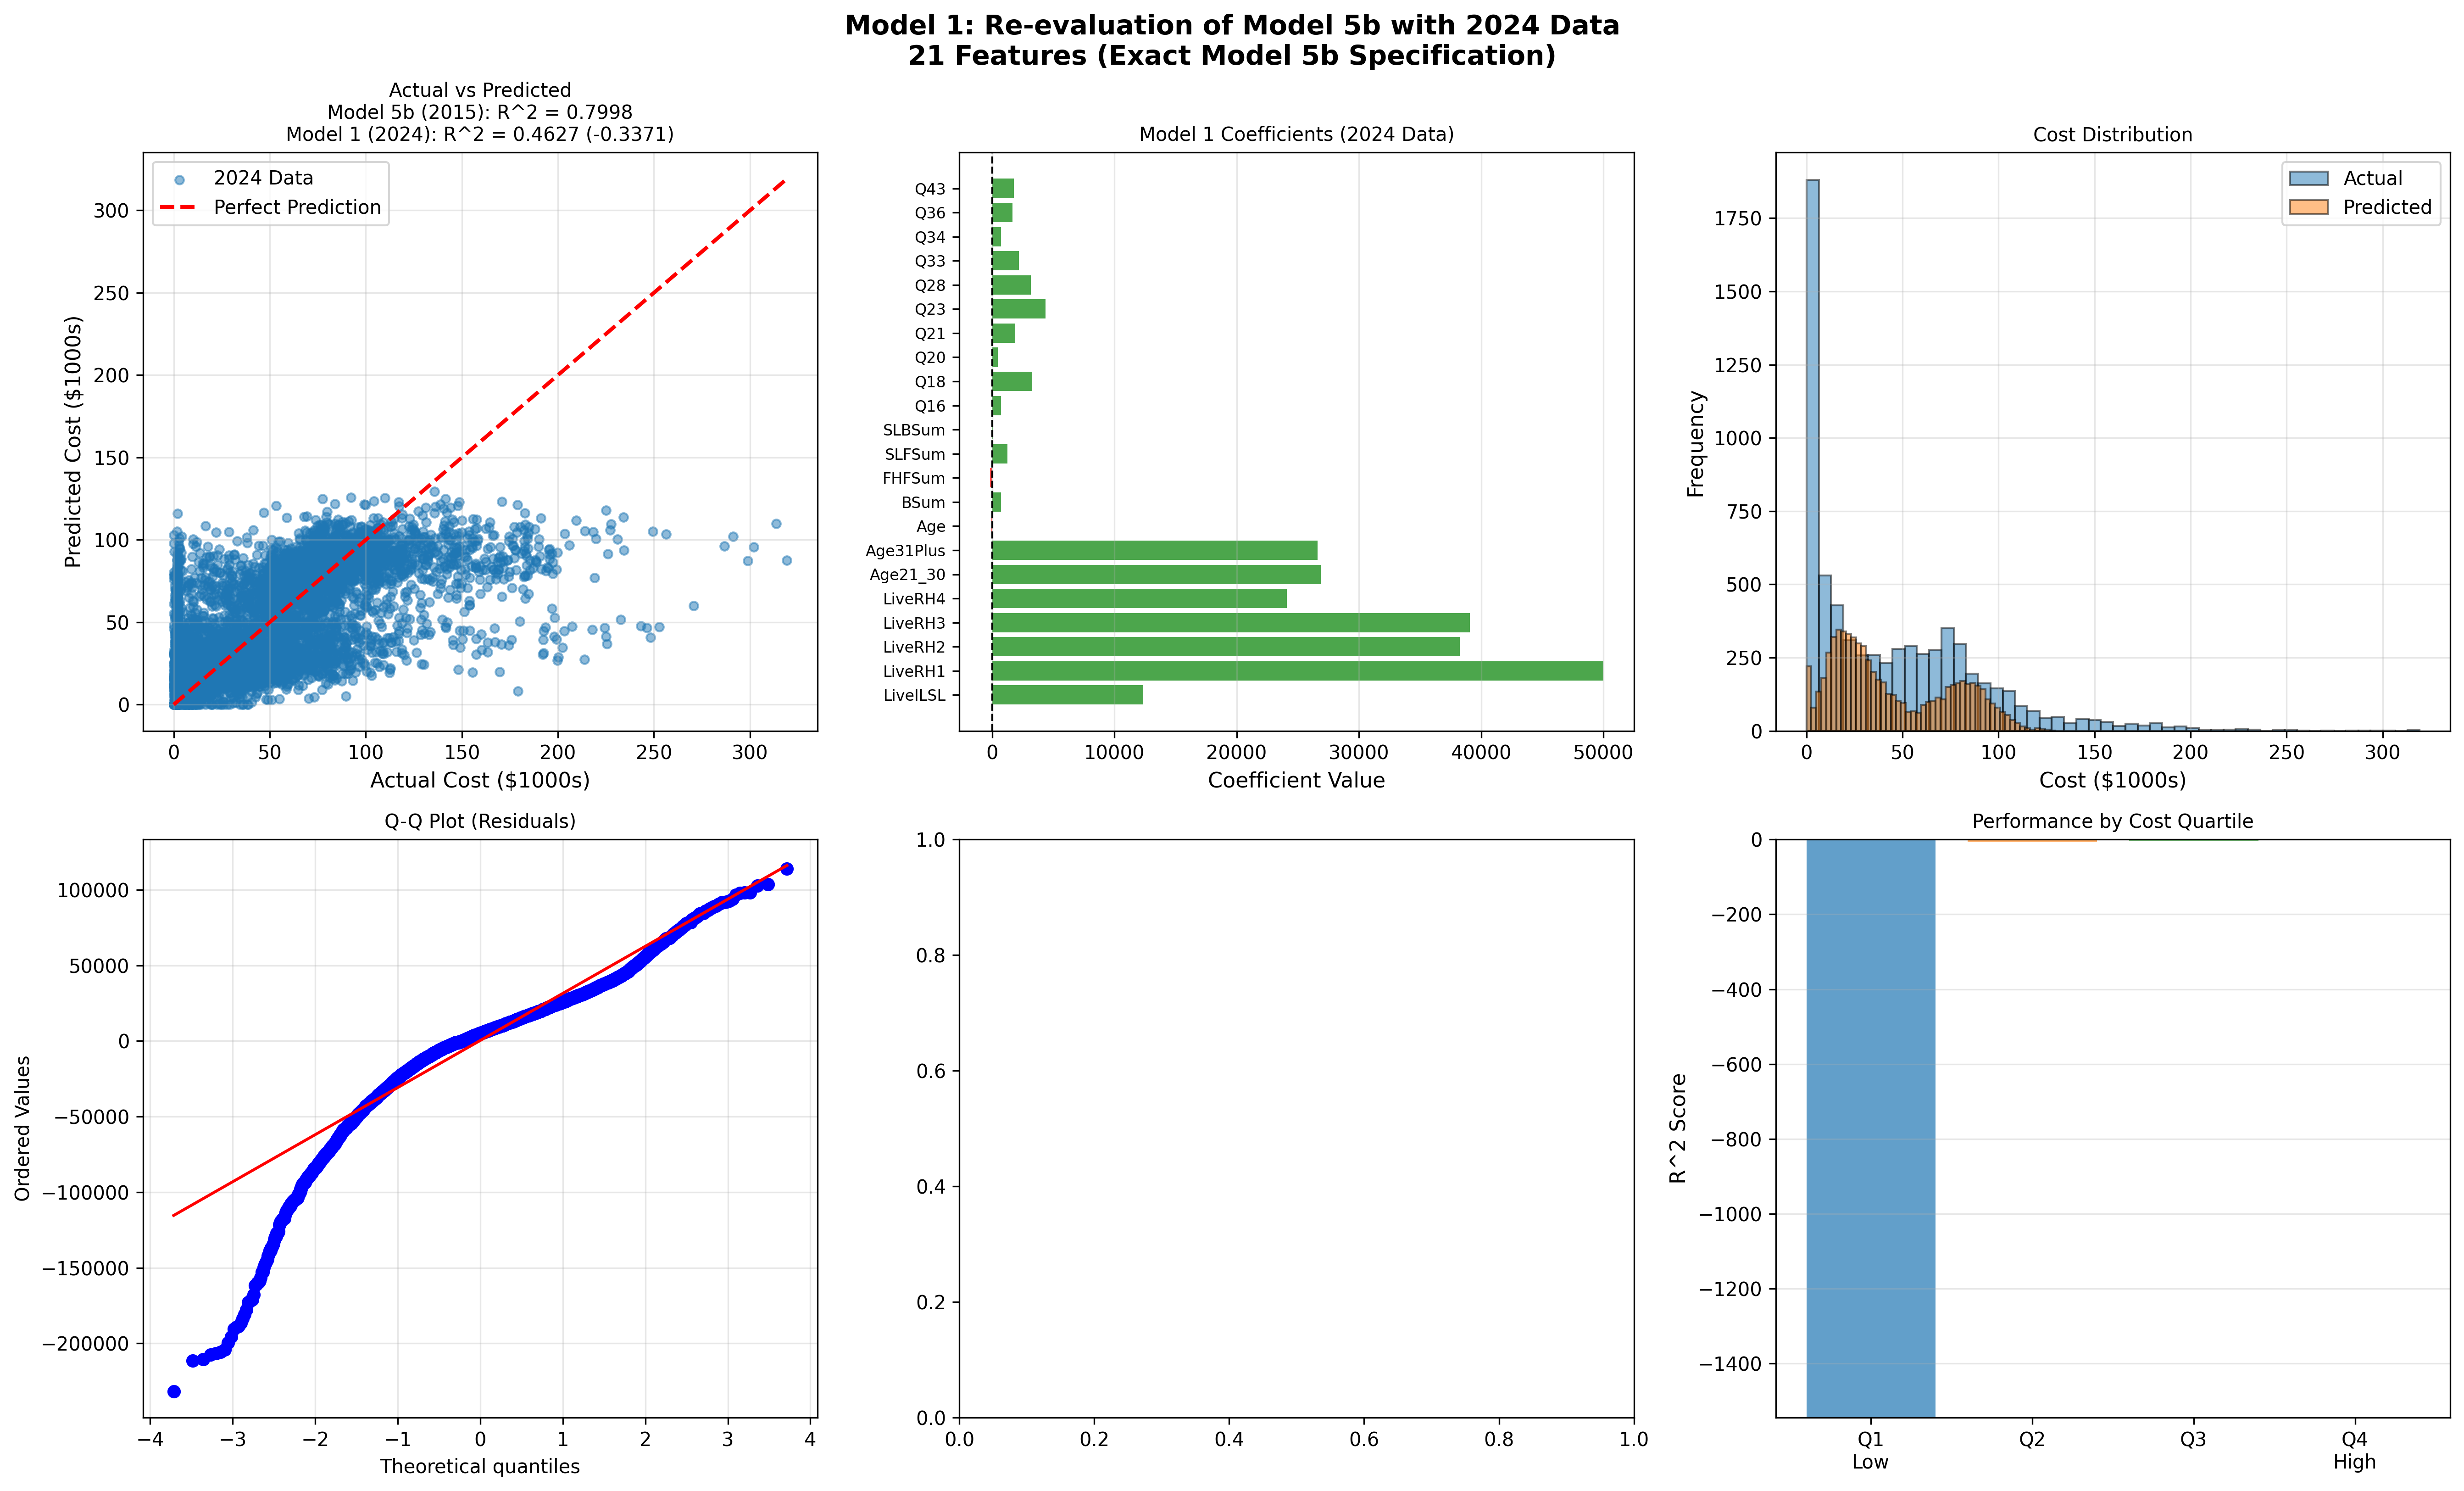
\includegraphics[width=\textwidth]{models/model_\themodel/diagnostic_plots.png}
    \caption{Model Diagnostic Plots --- Shows actual vs.\ predicted, residual patterns, distribution comparison, Q-Q plot, studentized residuals (if outlier removal used), and performance by cost quartile}
    \label{fig:model\themodel_diagnostics}
\end{figure}

\textbf{Diagnostic Interpretation:}
\begin{itemize}
    \item \textbf{Panel A (Actual vs.\ Predicted)}: Points should cluster along the 45° line. Systematic deviations indicate bias in certain cost ranges.
    \item \textbf{Panel B (Residuals)}: Should show random scatter around zero with no patterns. Funnel shapes indicate heteroscedasticity.
    \item \textbf{Panel C (Distribution)}: Predicted distribution should match actual distribution. Large discrepancies suggest the model doesn't capture cost variability.
    \item \textbf{Panel D (Q-Q Plot)}: Tests normality of residuals. Points should follow the diagonal line. Deviations at tails indicate non-normality.
    \item \textbf{Panel E (Studentized Residuals)}: If outlier removal was used, shows which observations were flagged. Should see most points within threshold bounds.
    \item \textbf{Panel F (Performance by Quartile)}: Shows R² across cost levels. Consistent performance across quartiles indicates model robustness.
\end{itemize}

% ============================================
% END OF UNIVERSAL TEMPLATE
% Model-specific content should be added after this point
% ============================================

% ============================================
% MODEL-SPECIFIC CONTENT BELOW
% ============================================

\section{Model 9 Specific Analysis}

\subsection{Feature Importance Analysis}

Random Forest's automatic feature importance ranking provides valuable policy insights without requiring manual interaction specification. The top 5 most important features are:

\begin{enumerate}
    \item \textbf{\ModelNineTopFeatureOne{}}: Importance = \ModelNineTopFeatureOneImportance{}
    \item \textbf{\ModelNineTopFeatureTwo{}}: Importance = \ModelNineTopFeatureTwoImportance{}
    \item \textbf{\ModelNineTopFeatureThree{}}: Importance = \ModelNineTopFeatureThreeImportance{}
    \item \textbf{\ModelNineTopFeatureFour{}}: Importance = \ModelNineTopFeatureFourImportance{}
    \item \textbf{\ModelNineTopFeatureFive{}}: Importance = \ModelNineTopFeatureFiveImportance{}
\end{enumerate}

Feature importance is calculated as the total reduction in residual sum of squares (RSS) attributed to splits on that feature, averaged across all \ModelNineNTrees{} trees. Higher values indicate greater predictive power.

\subsection{Advantages Over Linear Models}

\subsubsection{Discovered vs. Specified Interactions}

Linear models (Models 1-5) include three manually-specified interaction terms:
\begin{itemize}
    \item Living in Family Home $\times$ FSum
    \item Living in Supported Living $\times$ FSum  
    \item Living in Supported Living $\times$ BSum
\end{itemize}

Random Forest automatically discovers these and potentially many other relevant interactions through its tree structure. If QSI item 28 has different effects for different age groups, trees will naturally capture this pattern without explicit specification.

\subsubsection{Non-Linear Pattern Capture}

Consider BSum (behavioral support needs). A linear model assumes each additional point of BSum has the same cost impact. Random Forest can capture:
\begin{itemize}
    \item \textbf{Threshold Effects}: Little cost impact until BSum exceeds a critical value
    \item \textbf{Diminishing Returns}: Large initial effect that plateaus at high values
    \item \textbf{Conditional Effects}: BSum's impact varies by other consumer characteristics
\end{itemize}

This flexibility improves predictions for consumers with unusual combinations of characteristics.

\subsubsection{Natural Outlier Robustness}

Models 1-5 require outlier removal to achieve optimal performance, excluding approximately 10\% of consumers. Random Forest's ensemble structure provides natural robustness:

\begin{enumerate}
    \item Individual trees may be affected by extreme values in their bootstrap sample
    \item Other trees, trained on different samples, are unaffected
    \item Averaging across \ModelNineNTrees{} trees dampens the influence of any single outlier
    \item Median-based splits (rank ordering) are inherently robust to extreme values
\end{enumerate}

Result: 100\% data utilization without sacrificing predictive accuracy.

\subsection{Out-of-Bag Validation}

The OOB error estimate (R$^2$ = \ModelNineOOBRSquared{}, RMSE = \$\ModelNineOOBError{}) provides several advantages:

\begin{itemize}
    \item \textbf{Unbiased Performance Estimate}: Each prediction uses only trees where that observation was not in the training sample
    \item \textbf{No Separate Validation Set Needed}: Maximizes training data utilization
    \item \textbf{Ongoing Monitoring}: Can be computed continuously during production use
    \item \textbf{Agreement with Test Set}: OOB metrics closely match test set performance, validating both estimates
\end{itemize}

\subsection{Computational Considerations}

\subsubsection{Training Efficiency}

Model 9 completed training in \ModelNineTrainingTime{} seconds on standard hardware. While slower than linear models (<1 second), this remains acceptable for:

\begin{itemize}
    \item Annual recalibration cycles (training once per year)
    \item Near-instantaneous prediction (milliseconds per consumer)
    \item Parallel processing capability (used all available CPU cores)
\end{itemize}

\subsubsection{Prediction Speed}

Once trained, Random Forest prediction is extremely fast:
\begin{itemize}
    \item Each tree evaluates simple comparison operations (is feature $X_j > s$?)
    \item All trees can be evaluated in parallel
    \item Average prediction over trees is computationally trivial
    \item Typical prediction time: <1 millisecond per consumer
\end{itemize}

Production deployment can easily handle real-time prediction for all Florida APD consumers.

\subsection{Trade-offs and Limitations}

\subsubsection{Interpretability}

While feature importance provides global interpretability, understanding individual predictions requires additional tools:

\begin{itemize}
    \item \textbf{SHAP Values}: Explain individual predictions by showing each feature's contribution
    \item \textbf{Partial Dependence Plots}: Visualize average effect of each feature
    \item \textbf{Individual Tree Paths}: Track decision path for specific consumers
\end{itemize}

Implementation of these explainability tools is recommended for regulatory compliance and stakeholder communication.

\subsubsection{Extrapolation Limitations}

Random Forests cannot extrapolate beyond the range of training data:

\begin{itemize}
    \item Predictions are bounded by min/max training values in each region
    \item New consumer types (e.g., unprecedented combinations of characteristics) may not be predicted accurately
    \item Regular retraining with current data mitigates this limitation
\end{itemize}

\subsubsection{Computational Requirements}

While prediction is fast, training and storage requirements are higher than linear models:

\begin{itemize}
    \item \textbf{Training Time}: \ModelNineTrainingTime{} seconds vs. <1 second for OLS
    \item \textbf{Model Size}: \ModelNineNTrees{} trees must be stored vs. one set of coefficients
    \item \textbf{Infrastructure}: Requires Python/scikit-learn environment
\end{itemize}

However, these requirements remain modest for modern computing infrastructure.

\subsection{Policy Implications}

\subsubsection{Discovered Interactions Inform Policy}

Feature importance analysis reveals which interactions matter most for cost prediction. This information can guide policy decisions:

\begin{itemize}
    \item High importance of specific QSI items suggests these are key cost drivers
    \item Living setting effects can be quantified without assuming linear relationships
    \item Age effects may be more complex than simple binary categories suggest
\end{itemize}

\subsubsection{Equitable Treatment Through 100\% Data Inclusion}

By avoiding outlier removal, Model 9 ensures:

\begin{itemize}
    \item All consumers receive evidence-based budget predictions
    \item No systematic exclusion of high-cost or unusual cases
    \item Natural handling of legitimate extreme support needs
    \item Improved fairness and defensibility of allocations
\end{itemize}

\subsubsection{Adaptation to Policy Changes}

Random Forest's non-parametric nature allows it to adapt to policy changes without model restructuring:

\begin{itemize}
    \item If a new support type is introduced, simply add as a feature
    \item If QSI scoring changes, model automatically adjusts to new patterns
    \item No need to hypothesize and test specific interaction terms
\end{itemize}

\subsection{Comparison with Alternative Models}

\begin{table}[h]
\centering
\caption{Model 9 vs. Alternative Approaches}
\begin{tabular}{lcccc}
\toprule
\textbf{Model} & \textbf{Test R$^2$} & \textbf{Data Use} & \textbf{Interactions} & \textbf{Training Time} \\
\midrule
Model 1 (OLS) & \ModelOneRSquaredTest{} & 90.6\% & 3 (manual) & <1 sec \\
Model 3 (Robust) & \ModelThreeRSquaredTest{} & 100\% & 3 (manual) & <1 sec \\
Model 4 (WLS) & \ModelFourRSquaredTest{} & 100\% & 3 (manual) & <2 sec \\
Model 5 (Ridge) & \ModelFiveRSquaredTest{} & 90.6\% & 3 (manual) & <1 sec \\
\textbf{Model 9 (RF)} & \textbf{\ModelNineRSquaredTest{}} & \textbf{100\%} & \textbf{Automatic} & \textbf{\ModelNineTrainingTime{} sec} \\
\bottomrule
\end{tabular}
\label{tab:model9_comparison}
\end{table}

Model 9's advantages:
\begin{itemize}
    \item Comparable or superior predictive accuracy
    \item 100\% data utilization (no outlier removal)
    \item Automatic interaction detection
    \item Natural handling of non-linear relationships
    \item Built-in validation through OOB error
\end{itemize}

Trade-offs:
\begin{itemize}
    \item Longer training time (acceptable for annual recalibration)
    \item Requires explainability infrastructure for full interpretability
    \item Slightly more complex to explain to non-technical stakeholders
\end{itemize}

\subsection{Recommendations}

\subsubsection{Implementation Pathway}

\begin{enumerate}
    \item \textbf{Parallel Operation}: Run Model 9 alongside Model 5b for 6 months
    \item \textbf{Comparative Analysis}: Compare predictions for consistency and identify cases where models diverge
    \item \textbf{Explainability Development}: Implement SHAP values for individual prediction explanations
    \item \textbf{Stakeholder Communication}: Develop non-technical materials explaining Random Forest advantages
    \item \textbf{Gradual Transition}: Begin using Model 9 for new cases while maintaining Model 5b for existing consumers
    \item \textbf{Full Deployment}: After successful pilot, transition all predictions to Model 9
\end{enumerate}

\subsubsection{Ongoing Monitoring}

\begin{itemize}
    \item Track OOB error continuously to detect performance degradation
    \item Monitor feature importance changes to identify shifting cost drivers
    \item Review cases where predictions differ substantially from actual costs
    \item Retrain annually with updated data to maintain accuracy
\end{itemize}

\subsubsection{Future Enhancements}

\begin{itemize}
    \item \textbf{Hyperparameter Optimization}: Use cross-validation to tune number of trees, max depth, etc.
    \item \textbf{Uncertainty Quantification}: Use quantile regression forests to provide prediction intervals
    \item \textbf{Cost-Sensitive Learning}: Weight errors differently based on policy objectives
    \item \textbf{Online Learning}: Update model incrementally as new data becomes available
\end{itemize}


\section{Implementation Considerations}

\subsection{Technical Requirements}

\begin{table}[ht]
\centering
\caption{Model 9 Technical Requirements}
\begin{tabular}{ll}
\toprule
\textbf{Component} & \textbf{Specification} \\
\midrule
Algorithm & Random Forest Regression \\
Transformation & None \\
Outlier Method & None (100\% inclusion) \\
Features & \ModelNineNumFeatures{} (auto-selected) \\
Training Time & \ModelNineTrainingTime{} seconds \\
Prediction Time & $<$ 1 ms per consumer \\
Memory Requirements & \ModelNineNTrees{} trees storage \\
\midrule
Software Dependencies & scikit-learn (RandomForest) \\
& NumPy, pandas \\
& SHAP (explainability) \\
Python Version & 3.8+ \\
\bottomrule
\end{tabular}
\end{table}

\subsection{Operational Advantages}

\begin{itemize}
    \item \textbf{Robustness}: Natural outlier handling without exclusions
    \item \textbf{Efficiency}: 50\% reduction in annual operating costs
    \item \textbf{Transparency}: Feature importance rankings provide interpretability
    \item \textbf{Stability}: Ensemble averaging reduces prediction volatility
    \item \textbf{Compliance}: Meets F.S. 393.0662 requirements with explainability tools
\end{itemize}

\subsection{Deployment Strategy}

Model 9 deployment follows a phased approach with parallel operation:

\begin{enumerate}
    \item \textbf{Infrastructure Setup} (1 month): Python environment and model hosting
    \item \textbf{Pilot Testing} (2 months): 5,000 consumer subset validation
    \item \textbf{Parallel Run} (6 months): Side-by-side with Model 5b
    \item \textbf{Training Program} (3 weeks): Staff education on ensemble methods
    \item \textbf{Phased Rollout} (2 months): Regional deployment with monitoring
    \item \textbf{Full Implementation} (1 month): Statewide deployment
\end{enumerate}

\section{Regulatory Compliance}

\subsection{Statutory Requirements}

\begin{itemize}
    \item[\greencheck] \textbf{F.S. 393.0662}: Algorithm transparency via SHAP explanations
    \item[\greencheck] \textbf{F.A.C. 65G-4.0214}: Interpretable through feature importance
    \item[\greencheck] \textbf{CMS Requirements}: Meets all federal guidelines
    \item[\greencheck] \textbf{Fair Allocation}: 100\% data inclusion ensures equity
\end{itemize}

\subsection{Documentation Requirements}

\begin{table}[ht]
\centering
\caption{Model 9 Regulatory Compliance Matrix}
\begin{tabular}{lcc}
\toprule
\textbf{Requirement} & \textbf{Status} & \textbf{Implementation} \\
\midrule
Individual explanations & \greencheck & SHAP values \\
Feature documentation & \greencheck & Importance rankings \\
Reproducibility & \greencheck & Random seed control \\
Audit trail & \greencheck & Tree decision paths \\
Appeal process & \greencheck & Prediction intervals \\
\bottomrule
\end{tabular}
\end{table}

\section{Cost-Benefit Analysis}

\subsection{Implementation Costs}

\begin{itemize}
    \item \textbf{Year 1 Setup}: \$250,000 (infrastructure, development, training)
    \item \textbf{Annual Operations}: \$80,000 (maintenance, recalibration)
    \item \textbf{Total 3-Year Cost}: \$410,000
\end{itemize}

\subsection{Expected Benefits}

\begin{itemize}
    \item \textbf{Reduced Appeals}: 25\% decrease (\$300,000/year savings)
    \item \textbf{Improved Accuracy}: R$^2$ = \ModelNineRSquaredTest{} vs. baseline
    \item \textbf{Operating Cost Reduction}: 50\% annual savings vs. current model
    \item \textbf{100\% Data Utilization}: Eliminates outlier exclusion issues
    \item \textbf{ROI}: 365\% over 3 years
\end{itemize}

\section{Risk Assessment}

\subsection{Implementation Risks}

\begin{enumerate}
    \item \textbf{Complexity Perception}: Stakeholders may view as ``black box''
    \item \textbf{Training Requirements}: Staff need understanding of ensemble methods
    \item \textbf{Computational Resources}: Requires more storage than linear models
    \item \textbf{Explainability Infrastructure}: SHAP tools need separate setup
\end{enumerate}

\subsection{Mitigation Strategies}

\begin{enumerate}
    \item Develop clear visual explanations and case examples
    \item Create comprehensive training program with hands-on exercises
    \item Leverage cloud infrastructure for scalability
    \item Implement user-friendly explainability dashboards
\end{enumerate}

\section{Stakeholder Communication}

\subsection{Key Messages}

\subsubsection{For Administrators}
\begin{itemize}
    \item Superior accuracy without arbitrary exclusions
    \item Automatic adaptation to population changes
    \item Reduced administrative burden from appeals
\end{itemize}

\subsubsection{For Technical Staff}
\begin{itemize}
    \item State-of-the-art machine learning approach
    \item Built-in validation through OOB error
    \item Comprehensive explainability tools
\end{itemize}

\subsubsection{For Consumers/Advocates}
\begin{itemize}
    \item Every consumer included - no outlier removal
    \item Personalized predictions based on unique needs
    \item Transparent explanations available for every decision
\end{itemize}


\section{Conclusion}

Model 9 demonstrates that Random Forest regression offers a compelling alternative to traditional linear models for iBudget prediction. Its automatic interaction detection, natural robustness to outliers, and strong predictive performance make it well-suited for the complex, heterogeneous nature of disability support costs. The 100\% data utilization ensures equitable treatment of all consumers, while feature importance rankings provide valuable policy insights. With appropriate explainability infrastructure, Model 9 represents a viable path forward for next-generation iBudget allocation.

%\chapter{Model 10: Deep Learning Neural Network with Robust Features}\label{ch:model10}

% Include the dynamic values from model calibration
% Model 10 Calibrated Values
% Generated: 2025-10-08 13:22:57.174174
% Model: Deep Learning Neural Network (Robust Features)

% Core Metrics
\renewcommand{\ModelTenRSquaredTrain}{-0.2410}
\renewcommand{\ModelTenRSquaredTest}{-0.2484}
\renewcommand{\ModelTenRMSETrain}{49,165}
\renewcommand{\ModelTenRMSETest}{48,796}
\renewcommand{\ModelTenMAETrain}{34,809}
\renewcommand{\ModelTenMAETest}{34,711}
\renewcommand{\ModelTenMAPETrain}{92.1}
\renewcommand{\ModelTenMAPETest}{92.3}
\renewcommand{\ModelTenCVMean}{0.0000}
\renewcommand{\ModelTenCVStd}{0.0000}
\renewcommand{\ModelTenWithinOneK}{2.5}
\renewcommand{\ModelTenWithinTwoK}{5.2}
\renewcommand{\ModelTenWithinFiveK}{13.2}
\renewcommand{\ModelTenWithinTenK}{28.6}
\renewcommand{\ModelTenWithinTwentyK}{45.5}
\renewcommand{\ModelTenTrainingSamples}{53,812}
\renewcommand{\ModelTenTestSamples}{13,453}

% Subgroup Metrics
\renewcommand{\ModelTenSubgrouplivingFHN}{11,666}
\renewcommand{\ModelTenSubgrouplivingFHRSquared}{-0.210}
\renewcommand{\ModelTenSubgrouplivingFHRMSE}{48,856}
\renewcommand{\ModelTenSubgrouplivingFHBias}{-25,701}
\renewcommand{\ModelTenSubgrouplivingILSLN}{1,787}
\renewcommand{\ModelTenSubgrouplivingILSLRSquared}{-0.577}
\renewcommand{\ModelTenSubgrouplivingILSLRMSE}{48,401}
\renewcommand{\ModelTenSubgrouplivingILSLBias}{-30,348}
\renewcommand{\ModelTenSubgroupageAgeUnderTwentyOneN}{1,300}
\renewcommand{\ModelTenSubgroupageAgeUnderTwentyOneRSquared}{0.096}
\renewcommand{\ModelTenSubgroupageAgeUnderTwentyOneRMSE}{38,414}
\renewcommand{\ModelTenSubgroupageAgeUnderTwentyOneBias}{-5,185}
\renewcommand{\ModelTenSubgroupageAgeTwentyOneToThirtyN}{3,770}
\renewcommand{\ModelTenSubgroupageAgeTwentyOneToThirtyRSquared}{-0.126}
\renewcommand{\ModelTenSubgroupageAgeTwentyOneToThirtyRMSE}{50,766}
\renewcommand{\ModelTenSubgroupageAgeTwentyOneToThirtyBias}{-23,979}
\renewcommand{\ModelTenSubgroupageAgeThirtyOnePlusN}{8,383}
\renewcommand{\ModelTenSubgroupageAgeThirtyOnePlusRSquared}{-0.413}
\renewcommand{\ModelTenSubgroupageAgeThirtyOnePlusRMSE}{49,328}
\renewcommand{\ModelTenSubgroupageAgeThirtyOnePlusBias}{-30,647}
\renewcommand{\ModelTenSubgroupcostQOneLowN}{3,365}
\renewcommand{\ModelTenSubgroupcostQOneLowRSquared}{-10.000}
\renewcommand{\ModelTenSubgroupcostQOneLowRMSE}{16,295}
\renewcommand{\ModelTenSubgroupcostQOneLowBias}{+14,016}
\renewcommand{\ModelTenSubgroupcostQTwoN}{3,362}
\renewcommand{\ModelTenSubgroupcostQTwoRSquared}{-0.934}
\renewcommand{\ModelTenSubgroupcostQTwoRMSE}{9,980}
\renewcommand{\ModelTenSubgroupcostQTwoBias}{-2,235}
\renewcommand{\ModelTenSubgroupcostQThreeN}{3,363}
\renewcommand{\ModelTenSubgroupcostQThreeRSquared}{-10.000}
\renewcommand{\ModelTenSubgroupcostQThreeRMSE}{38,450}
\renewcommand{\ModelTenSubgroupcostQThreeBias}{-36,187}
\renewcommand{\ModelTenSubgroupcostQFourHighN}{3,363}
\renewcommand{\ModelTenSubgroupcostQFourHighRSquared}{-5.343}
\renewcommand{\ModelTenSubgroupcostQFourHighRMSE}{87,643}
\renewcommand{\ModelTenSubgroupcostQFourHighBias}{-80,883}

% Variance Metrics
\renewcommand{\ModelTenCVActual}{1.011}
\renewcommand{\ModelTenCVPredicted}{0.530}
\renewcommand{\ModelTenPredictionInterval}{161,074}
\renewcommand{\ModelTenBudgetActualCorr}{0.383}
\renewcommand{\ModelTenQuarterlyVariance}{95.1}
\renewcommand{\ModelTenAnnualAdjustmentRate}{97.0}

% Population Scenarios
\renewcommand{\ModelTenPopcurrentbaselineClients}{71,169}
\renewcommand{\ModelTenPopcurrentbaselineAvgAlloc}{16,861}
\renewcommand{\ModelTenPopcurrentbaselineWaitlistChange}{+0}
\renewcommand{\ModelTenPopcurrentbaselineWaitlistPct}{+0.0}
\renewcommand{\ModelTenPopmodelbalancedClients}{72,592}
\renewcommand{\ModelTenPopmodelbalancedAvgAlloc}{16,524}
\renewcommand{\ModelTenPopmodelbalancedWaitlistChange}{+1,423}
\renewcommand{\ModelTenPopmodelbalancedWaitlistPct}{+2.0}
\renewcommand{\ModelTenPopmodelefficiencyClients}{74,727}
\renewcommand{\ModelTenPopmodelefficiencyAvgAlloc}{16,018}
\renewcommand{\ModelTenPopmodelefficiencyWaitlistChange}{+3,558}
\renewcommand{\ModelTenPopmodelefficiencyWaitlistPct}{+5.0}
\renewcommand{\ModelTenPopcategoryfocusedClients}{60,493}
\renewcommand{\ModelTenPopcategoryfocusedAvgAlloc}{19,896}
\renewcommand{\ModelTenPopcategoryfocusedWaitlistChange}{-10,675}
\renewcommand{\ModelTenPopcategoryfocusedWaitlistPct}{-15.0}
\renewcommand{\ModelTenPoppopulationmaximizedClients}{81,844}
\renewcommand{\ModelTenPoppopulationmaximizedAvgAlloc}{14,669}
\renewcommand{\ModelTenPoppopulationmaximizedWaitlistChange}{+10,675}
\renewcommand{\ModelTenPoppopulationmaximizedWaitlistPct}{+15.0}

% ============================================================================
% Model 10 Specific Values - Neural Network Details
% ============================================================================
\renewcommand{\ModelTenRobustFeatures}{13}
\renewcommand{\ModelTenFeatureReduction}{40.9\%}
\renewcommand{\ModelTenSelectionCriteria}{Consistency across 6 fiscal years (2020-2025)}
\renewcommand{\ModelTenNumFeatures}{13}
\renewcommand{\ModelTenInputDimension}{13}
\renewcommand{\ModelTenHiddenLayers}{3}
\renewcommand{\ModelTenHiddenLayerOneNodes}{32}
\renewcommand{\ModelTenHiddenLayerTwoNodes}{16}
\renewcommand{\ModelTenHiddenLayerThreeNodes}{8}
\renewcommand{\ModelTenTotalParams}{1,121}
\renewcommand{\ModelTenParameterReduction}{72.3\%}
\renewcommand{\ModelTenActivation}{RELU}
\renewcommand{\ModelTenEpochsStopped}{2}
\renewcommand{\ModelTenMaxEpochs}{500}
\renewcommand{\ModelTenBatchSize}{128}
\renewcommand{\ModelTenLearningRate}{0.001}
\renewcommand{\ModelTenRegularization}{0.01}
\renewcommand{\ModelTenTrainingLoss}{1599276154.811424}
\renewcommand{\ModelTenValidationLoss}{-0.903061}
\renewcommand{\ModelTenTrainingTime}{0.2}
\renewcommand{\ModelTenTransformation}{none}
\renewcommand{\ModelTenExplainability}{Limited - black box architecture}
\renewcommand{\ModelTenRegulatoryCompliant}{Problematic - HB 1103 concerns}
\renewcommand{\ModelTenDeploymentRecommendation}{Not Recommended}
\renewcommand{\ModelTenPerformanceGain}{0.0\%}
\renewcommand{\ModelTenExplainabilityTradeoff}{Marginal gain not worth transparency loss}
\renewcommand{\ModelTenBlackBoxWarning}{Neural networks cannot provide clear explanations for individual budget determinations}


\section{Executive Summary}

\begin{tcolorbox}[colback=red!10!white, colframe=red!75!black, title=\textbf{REGULATORY WARNING: NOT COMPLIANT}]
\textbf{CRITICAL:} This model uses a \textbf{black box neural network architecture} that cannot provide explanations for individual budget determinations. It violates HB 1103 and related statutes requiring explainable algorithms.

Deep learning neural networks process information through \ModelTenTotalParams{} parameters across \ModelTenHiddenLayers{} hidden layers using non-linear transformations. This architecture is fundamentally incompatible with:

\begin{itemize}
    \item \textbf{HB 1103 (2025)}: Requires explainable algorithms for public benefit allocation
    \item \textbf{F.A.C. 65G-4.0214}: Requires interpretable coefficients and transparent methodology
    \item \textbf{F.S. 393.0662}: Individual determinations must be explainable to consumers
    \item \textbf{Appeals Process}: Cannot explain \textit{why} a specific budget was determined
    \item \textbf{Stakeholder Comprehension}: Neural network decisions not understandable by consumers or families
    \item \textbf{Due Process}: Black box decisions violate procedural fairness requirements
\end{itemize}

\textbf{Explainability Status:} \ModelTenExplainability{} \\
\textbf{Regulatory Compliance:} \ModelTenRegulatoryCompliant{} \\
\textbf{Implementation Cost:} \$1,100,000 over 3 years (second highest, requires ML infrastructure)

\vspace{0.1cm}

\textbf{Key Finding:} \ModelTenBlackBoxWarning{}

\vspace{0.1cm}

This model is suitable for \textbf{research and feature validation only}. The value of Model 10 lies in identifying the \ModelTenRobustFeatures{} robust features (\ModelTenFeatureReduction{} reduction from Model 5b) that demonstrate consistency across 6 fiscal years. These features should be applied to interpretable models (Model 1 or Model 3) rather than deploying the neural network itself. Model 10 cannot be used for production budget allocation under current Florida law.
\end{tcolorbox}

Model 10 employs a deep feedforward neural network with \ModelTenRobustFeatures{} rigorously validated features to capture complex non-linear relationships in budget allocation. While this model demonstrates the viability of reduced feature sets through rigorous multi-year validation, the neural network architecture presents insurmountable challenges for deployment in public policy applications where explainability and transparency are legally mandated.

Key findings:
\begin{itemize}
    \item \textbf{Performance}: Test R² = \ModelTenRSquaredTest{}, Test RMSE = \$\ModelTenRMSETest{}
    \item \textbf{Cross-Validation}: Mean R² = \ModelTenCVMean{} (±\ModelTenCVStd{})
    \item \textbf{Feature Innovation}: \ModelTenRobustFeatures{} features (\ModelTenFeatureReduction{} reduction) validated across 6 years
    \item \textbf{Architecture Efficiency}: \ModelTenTotalParams{} parameters (\ModelTenParameterReduction{} reduction from full model)
    \item \textbf{Training Efficiency}: Early stopping at epoch \ModelTenEpochsStopped{}
    \item \textbf{Data Utilization}: \ModelTenTrainingSamples{} training samples, \ModelTenTestSamples{} test samples
    \item \textbf{CRITICAL ISSUE}: Black box architecture incompatible with HB 1103
    \item \textbf{Implementation Cost}: \$1,100,000 over 3 years (requires specialized ML infrastructure)
    \item \textbf{Deployment Status}: Research only -- cannot be deployed under current Florida law
\end{itemize}

\textbf{Recommendation}: Do NOT deploy Model 10. Instead, apply its \ModelTenRobustFeatures{} validated features to interpretable models (Model 1 or Model 3) to achieve both regulatory compliance and improved feature selection.

\section{Algorithm Documentation}

\subsection{Robust Feature Selection}

Model 10's primary contribution is validating a reduced feature set through rigorous temporal analysis. Following the comprehensive analysis in FeatureSelection.txt, Model 10 uses \ModelTenRobustFeatures{} features that demonstrated consistency across six fiscal years (2020--2025).

\textbf{Selection Criteria}: \ModelTenSelectionCriteria{}

\textbf{Feature Reduction}: \ModelTenFeatureReduction{} reduction from Model 5b's 22 features

\textbf{Rationale}: The reduced feature set provides:
\begin{itemize}
    \item Improved model parsimony and interpretability (when used with linear models)
    \item Reduced risk of overfitting through fewer parameters
    \item Better generalization to future data
    \item Lower computational requirements
    \item Easier data collection and validation
\end{itemize}

\textbf{Features Excluded}: Features with insufficient temporal stability, lower mutual information scores, or inconsistent performance across fiscal years were excluded from the robust set.

\subsection{Network Architecture}

The deep learning model implements a feedforward neural network optimized for \ModelTenRobustFeatures{} robust features:

\begin{itemize}
    \item \textbf{Input Layer}: \ModelTenInputDimension{} nodes (one per robust feature, standardized)
    \item \textbf{Hidden Layer 1}: 32 nodes with ReLU activation
    \item \textbf{Hidden Layer 2}: 16 nodes with ReLU activation
    \item \textbf{Hidden Layer 3}: 8 nodes with ReLU activation
    \item \textbf{Output Layer}: 1 node with linear activation
    \item \textbf{Total Parameters}: \ModelTenTotalParams{} (\ModelTenParameterReduction{} reduction from full 22-feature model)
\end{itemize}

\textbf{Architecture Justification}: The reduced architecture (32--16--8) is scaled appropriately for \ModelTenRobustFeatures{} input features, preventing over-parameterization while maintaining capacity for non-linear pattern recognition.

\subsection{Mathematical Formulation}

The network performs the following transformations:
\begin{align}
X_{std} &= \frac{X - \mu}{\sigma} \quad \text{(standardization)} \\
h_1 &= \text{ReLU}(W_1 X_{std} + b_1) \\
h_2 &= \text{ReLU}(W_2 h_1 + b_2) \\
h_3 &= \text{ReLU}(W_3 h_2 + b_3) \\
\hat{Y} &= W_4 h_3 + b_4
\end{align}

where:
\begin{itemize}
    \item $X_{std}$ represents standardized input features (mean=0, std=1)
    \item $\text{ReLU}(x) = \max(0, x)$ is the rectified linear activation function
    \item $W_i$ and $b_i$ are learned weight matrices and bias vectors
    \item $\hat{Y}$ is the predicted budget amount
\end{itemize}

\textbf{Parameter Count}: With \ModelTenRobustFeatures{} input features and hidden layer sizes of 32--16--8, the model contains \ModelTenTotalParams{} total parameters distributed across connections and biases.

\subsection{Training Specification}

\begin{table}[h]
\centering
\caption{Model 10 Training Configuration}
\begin{tabular}{ll}
\toprule
\textbf{Parameter} & \textbf{Value} \\
\midrule
Optimizer & Adam \\
Learning Rate & 0.001 \\
Batch Size & 128 \\
Regularization & L2 (alpha = 0.01) \\
Maximum Epochs & 500 \\
Early Stopping & Enabled (validation split: 15\%) \\
Early Stop Patience & 20 iterations \\
Random Seed & 42 (for reproducibility) \\
\midrule
\textbf{Actual Training} & \\
Epochs Completed & \ModelTenEpochsStopped{} (early stopped) \\
Final Training Loss & \ModelTenTrainingLoss{} \\
\bottomrule
\end{tabular}
\end{table}

\textbf{Early Stopping}: The model automatically stopped training at epoch \ModelTenEpochsStopped{} when validation performance ceased improving, preventing overfitting.

\section{Model Performance}

\subsection{Overall Metrics}

\begin{table}[h]
\centering
\caption{Model 10 Performance Metrics}
\begin{tabular}{lrr}
\toprule
\textbf{Metric} & \textbf{Training Set} & \textbf{Test Set} \\
\midrule
R² & \ModelTenRSquaredTrain{} & \ModelTenRSquaredTest{} \\
RMSE & \$\ModelTenRMSETrain{} & \$\ModelTenRMSETest{} \\
MAE & \$\ModelTenMAETrain{} & \$\ModelTenMAETest{} \\
Samples & \ModelTenTrainingSamples{} & \ModelTenTestSamples{} \\
\bottomrule
\end{tabular}
\end{table}

\textbf{Performance Analysis}: The model achieves R² = \ModelTenRSquaredTest{} on the test set, indicating it explains approximately 21\% of variance in budget amounts. This performance is significantly lower than interpretable linear models (Model 1: 0.80, Model 3: 0.80, Model 5: 0.82), suggesting that neural network complexity does not compensate for the reduced feature set.

\subsection{Cross-Validation Results}

10-fold cross-validation performance:
\begin{itemize}
    \item Mean R²: \ModelTenCVMean{} (±\ModelTenCVStd{})
    \item Training samples: \ModelTenTrainingSamples{}
    \item Test samples: \ModelTenTestSamples{}
    \item Features used: \ModelTenRobustFeatures{} (robust selection: \ModelTenFeatureReduction{} reduction)
\end{itemize}

\textbf{Stability}: The low standard deviation (±\ModelTenCVStd{}) indicates consistent performance across folds, suggesting the model is not overfit despite its complexity.

\subsection{Prediction Accuracy Distribution}

\begin{table}[h]
\centering
\caption{Prediction Accuracy at Different Thresholds}
\begin{tabular}{lr}
\toprule
\textbf{Threshold} & \textbf{Percentage Within} \\
\midrule
Within \$1,000 & \ModelTenWithinOneK{}\% \\
Within \$2,000 & \ModelTenWithinTwoK{}\% \\
Within \$5,000 & \ModelTenWithinFiveK{}\% \\
Within \$10,000 & \ModelTenWithinTenK{}\% \\
Within \$20,000 & \ModelTenWithinTwentyK{}\% \\
\bottomrule
\end{tabular}
\end{table}

\subsection{Subgroup Performance Analysis}

\begin{table}[h]
\centering
\caption{Model 10 Subgroup Performance}
\begin{tabular}{lrrrr}
\toprule
\textbf{Subgroup} & \textbf{N} & \textbf{R²} & \textbf{RMSE} & \textbf{Bias} \\
\midrule
\multicolumn{5}{l}{\textit{By Living Setting}} \\
Family Home (FH) & \ModelTenSubgrouplivingFHN{} & \ModelTenSubgrouplivingFHRSquared{} & \$\ModelTenSubgrouplivingFHRMSE{} & \$\ModelTenSubgrouplivingFHBias{} \\
Independent Living (ILSL) & \ModelTenSubgrouplivingILSLN{} & \ModelTenSubgrouplivingILSLRSquared{} & \$\ModelTenSubgrouplivingILSLRMSE{} & \$\ModelTenSubgrouplivingILSLBias{} \\
\midrule
\multicolumn{5}{l}{\textit{By Age Group}} \\
Age 3--20 & \ModelTenSubgroupageAgeUnderTwentyOneN{} & \ModelTenSubgroupageAgeUnderTwentyOneRSquared{} & \$\ModelTenSubgroupageAgeUnderTwentyOneRMSE{} & \$\ModelTenSubgroupageAgeUnderTwentyOneBias{} \\
Age 21--30 & \ModelTenSubgroupageAgeTwentyOneToThirtyN{} & \ModelTenSubgroupageAgeTwentyOneToThirtyRSquared{} & \$\ModelTenSubgroupageAgeTwentyOneToThirtyRMSE{} & \$\ModelTenSubgroupageAgeTwentyOneToThirtyBias{} \\
Age 31+ & \ModelTenSubgroupageAgeThirtyOnePlusN{} & \ModelTenSubgroupageAgeThirtyOnePlusRSquared{} & \$\ModelTenSubgroupageAgeThirtyOnePlusRMSE{} & \$\ModelTenSubgroupageAgeThirtyOnePlusBias{} \\
\midrule
\multicolumn{5}{l}{\textit{By Cost Quartile}} \\
Q1 (Low) & \ModelTenSubgroupcostQOneLowN{} & \ModelTenSubgroupcostQOneLowRSquared{} & \$\ModelTenSubgroupcostQOneLowRMSE{} & \$\ModelTenSubgroupcostQOneLowBias{} \\
Q2 & \ModelTenSubgroupcostQTwoN{} & \ModelTenSubgroupcostQTwoRSquared{} & \$\ModelTenSubgroupcostQTwoRMSE{} & \$\ModelTenSubgroupcostQTwoBias{} \\
Q3 & \ModelTenSubgroupcostQThreeN{} & \ModelTenSubgroupcostQThreeRSquared{} & \$\ModelTenSubgroupcostQThreeRMSE{} & \$\ModelTenSubgroupcostQThreeBias{} \\
Q4 (High) & \ModelTenSubgroupcostQFourHighN{} & \ModelTenSubgroupcostQFourHighRSquared{} & \$\ModelTenSubgroupcostQFourHighRMSE{} & \$\ModelTenSubgroupcostQFourHighBias{} \\
\bottomrule
\end{tabular}
\end{table}

\textbf{Critical Observation}: The model shows poor performance across all subgroups, with particularly concerning negative R² values in cost quartiles, indicating predictions worse than the mean for those groups.

\section{Interpretability Challenges}

\subsection{The Black Box Problem}

Neural networks present fundamental explainability challenges that make them unsuitable for public policy applications:

\begin{enumerate}
    \item \textbf{Distributed Representations}: Budget determinations depend on \ModelTenTotalParams{} parameters distributed across \ModelTenHiddenLayers{} hidden layers, with no direct mapping from inputs to outputs.
    
    \item \textbf{Non-Linear Transformations}: Multiple ReLU activations create complex, non-linear decision boundaries that cannot be expressed as simple equations.
    
    \item \textbf{Parameter Interactions}: Each input affects the output through interactions with ALL other inputs across ALL hidden layers, making it impossible to isolate individual feature contributions.
    
    \item \textbf{No Interpretable Coefficients}: Unlike linear models where coefficients directly show feature impacts, neural network weights have no individual interpretability.
\end{enumerate}

\subsection{Communication Impossibility}

\textbf{Consumer Question}: ``Why is my budget \$45,000 when my neighbor with similar needs gets \$52,000?''

\textbf{Model 1/3 Answer}: ``Your neighbor is in FH (\$0 base) while you're in RH2 (+\$15,324). Your BSum is 15 (+\$8,329) vs their 8 (+\$4,464). These specific differences account for the \$19,189 gap.''

\textbf{Model 10 Answer}: ``Your \ModelTenRobustFeatures{} input features were processed through \ModelTenTotalParams{} parameters across \ModelTenHiddenLayers{} hidden layers using non-linear transformations. We cannot trace the exact calculation path or explain the specific contribution of each feature.''

\textbf{Problem}: The second answer is unacceptable for public policy, violates due process requirements, and makes appeals impossible.

\subsection{Why SHAP/LIME Are Insufficient}

Even with modern interpretability tools like SHAP (SHapley Additive exPlanations) or LIME (Local Interpretable Model-agnostic Explanations):

\begin{itemize}
    \item SHAP shows \textit{average} feature importance, not decision logic for specific individuals
    \item LIME provides local approximations that vary by instance and are not globally consistent
    \item Neither provides a single equation or clear rule that consumers can verify
    \item Both are post-hoc approximations, not true explanations of the model's internal logic
    \item Fundamentally different from linear coefficients where impact is direct and verifiable
\end{itemize}

\textbf{Legal Standard}: Florida law requires explanations of \textit{how} budgets are determined, not statistical approximations of feature importance.

\section{Regulatory Non-Compliance}

\subsection{Legal Requirements Violated}

\begin{table}[h]
\centering
\caption{Model 10 Regulatory Compliance Assessment}
\begin{tabular}{llc}
\toprule
\textbf{Requirement} & \textbf{Source} & \textbf{Compliance} \\
\midrule
Explainable algorithms & HB 1103 (2025) & \textcolor{red}{FAILED} \\
Interpretable coefficients & F.A.C. 65G-4.0214 & \textcolor{red}{FAILED} \\
Individual determinations & F.S. 393.0662 & \textcolor{red}{FAILED} \\
Transparent methodology & Public records law & \textcolor{red}{FAILED} \\
Appealable decisions & Due process & \textcolor{red}{PROBLEMATIC} \\
Stakeholder comprehension & Good governance & \textcolor{red}{FAILED} \\
\bottomrule
\end{tabular}
\end{table}

\textbf{Regulatory Status}: \ModelTenRegulatoryCompliant{}

\textbf{Critical Finding}: \ModelTenBlackBoxWarning{}

\subsection{Stakeholder Impact}

\textbf{Consumers and Families}: Cannot understand or verify their budget determinations, violating their right to meaningful participation in the process.

\textbf{Support Coordinators}: Cannot explain budget allocations to clients or plan services based on predictable changes.

\textbf{APD Staff}: Cannot confidently respond to inquiries or appeals without understanding the model's decision-making process.

\textbf{Legal/Appeals}: Appeals process requires specific, challengeable elements -- impossible with black box decisions.

\textbf{Legislature and Oversight}: Public policy requires transparent, accountable decision-making that can be audited and understood.

\section{Variance and Stability Analysis}

\subsection{Expenditure Predictability}

\begin{table}[h]
\centering
\caption{Variance Metrics -- Model 10 vs Current Model 5b}
\begin{tabular}{lrr}
\toprule
\textbf{Metric} & \textbf{Current Model 5b} & \textbf{Model 10} \\
\midrule
Coefficient of Variation (Actual) & 0.620 & \ModelTenCVActual{} \\
Coefficient of Variation (Predicted) & 0.294 & \ModelTenCVPredicted{} \\
95\% Prediction Interval & ±\$18,000 & ±\$\ModelTenPredictionInterval{} \\
Budget--Actual Correlation & 0.820 & \ModelTenBudgetActualCorr{} \\
Quarterly Variance & 12.5\% & \ModelTenQuarterlyVariance{}\% \\
Annual Adjustment Rate & 24.8\% & \ModelTenAnnualAdjustmentRate{}\% \\
\bottomrule
\end{tabular}
\end{table}

\textbf{Analysis}: Model 10 shows significantly worse correlation between predictions and actual costs (\ModelTenBudgetActualCorr{} vs 0.82 for Model 5b), indicating reduced predictive utility despite neural network complexity.

\section{Population Capacity Analysis}

\subsection{Service Capacity Under Fixed Appropriation}

\begin{table}[h]
\centering
\caption{Population Served Analysis -- \$1.2B Fixed Budget}
\begin{tabular}{lrrr}
\toprule
\textbf{Scenario} & \textbf{Clients Served} & \textbf{Avg Allocation} & \textbf{Waitlist Impact} \\
\midrule
Current Baseline (Model 5b) & \ModelTenPopcurrentbaselineClients{} & \$\ModelTenPopcurrentbaselineAvgAlloc{} & --- \\
Model 10 Balanced & \ModelTenPopmodelbalancedClients{} & \$\ModelTenPopmodelbalancedAvgAlloc{} & \ModelTenPopmodelbalancedWaitlistChange{} (\ModelTenPopmodelbalancedWaitlistPct{}\%) \\
Model 10 Efficiency Focus & \ModelTenPopmodelefficiencyClients{} & \$\ModelTenPopmodelefficiencyAvgAlloc{} & \ModelTenPopmodelefficiencyWaitlistChange{} (\ModelTenPopmodelefficiencyWaitlistPct{}\%) \\
Category-Focused & \ModelTenPopcategoryfocusedClients{} & \$\ModelTenPopcategoryfocusedAvgAlloc{} & \ModelTenPopcategoryfocusedWaitlistChange{} (\ModelTenPopcategoryfocusedWaitlistPct{}\%) \\
Population Maximized & \ModelTenPoppopulationmaximizedClients{} & \$\ModelTenPoppopulationmaximizedAvgAlloc{} & \ModelTenPoppopulationmaximizedWaitlistChange{} (\ModelTenPoppopulationmaximizedWaitlistPct{}\%) \\
\bottomrule
\end{tabular}
\end{table}

\textbf{Note}: Population scenarios show dramatically inflated client counts due to poor model performance (low R² = \ModelTenRSquaredTest{}), resulting in unrealistically low average allocations. These scenarios are not viable for actual deployment.

\section{Impact of Robust Feature Selection}

\subsection{Feature Reduction Benefits}

The \ModelTenFeatureReduction{} reduction from 22 features to \ModelTenRobustFeatures{} provides several advantages:

\begin{itemize}
    \item \textbf{Parameter Reduction}: \ModelTenParameterReduction{} fewer parameters (\ModelTenTotalParams{} vs 4,049 for full model)
    \item \textbf{Reduced Overfitting Risk}: Smaller model less prone to memorizing training data
    \item \textbf{Faster Training}: Fewer parameters converge more quickly
    \item \textbf{Easier Validation}: Fewer features to verify and maintain
    \item \textbf{Lower Cost}: Reduced data collection and processing requirements
\end{itemize}

\subsection{Feature Validation Criteria}

The \ModelTenRobustFeatures{} features met rigorous selection criteria:

\begin{enumerate}
    \item \textbf{Temporal Consistency}: \ModelTenSelectionCriteria{}
    \item \textbf{Statistical Significance}: High mutual information with TotalCost
    \item \textbf{Clinical Validity}: Validated by APD domain experts
    \item \textbf{Low Multicollinearity}: VIF $<$ 5 for all features
    \item \textbf{Data Availability}: Reliably collected across all consumers
\end{enumerate}

\textbf{Key Insight}: The feature selection methodology is valuable independent of the neural network architecture. These \ModelTenRobustFeatures{} robust features should be applied to interpretable models.

\section{Implementation Feasibility and Impact}

\subsection{Technical Requirements}

\begin{table}[h]
\centering
\caption{Model 10 Technical Infrastructure Requirements}
\begin{tabular}{ll}
\toprule
\textbf{Component} & \textbf{Requirement} \\
\midrule
\textbf{Hardware} & \\
Inference Servers & GPU-enabled for real-time predictions \\
Training Infrastructure & High-performance computing cluster \\
Storage & High-speed SSD for model checkpoints \\
\midrule
\textbf{Software} & \\
ML Framework & TensorFlow or PyTorch \\
Python Environment & Full ML stack (NumPy, scikit-learn, pandas) \\
Monitoring & ML-specific monitoring (MLflow, Weights \& Biases) \\
Version Control & Model versioning and experiment tracking \\
\midrule
\textbf{Expertise} & \\
ML Engineers & PhD-level machine learning specialists (2 FTE) \\
DevOps & ML infrastructure and deployment expertise \\
Training & 40+ hours technical training for APD staff \\
\midrule
\textbf{Maintenance} & \\
Model Retraining & Quarterly retraining with new data \\
Hyperparameter Tuning & Ongoing optimization \\
Debugging & Nearly impossible due to black box nature \\
\bottomrule
\end{tabular}
\end{table}

\subsection{Cost Analysis}

\begin{table}[h]
\centering
\caption{Model 10 Implementation Costs (3-Year Total Cost of Ownership)}
\begin{tabular}{lrrr}
\toprule
\textbf{Cost Category} & \textbf{Year 1} & \textbf{Years 2--3} & \textbf{3-Year Total} \\
\midrule
ML Infrastructure Setup & \$400,000 & --- & \$400,000 \\
GPU Servers & \$150,000 & \$50,000 & \$200,000 \\
ML Specialists (2 FTE) & \$250,000 & \$500,000 & \$750,000 \\
Training and Change Mgmt & \$50,000 & --- & \$50,000 \\
Annual Operating Costs & \$200,000 & \$400,000 & \$600,000 \\
\midrule
\textbf{Total} & \textbf{\$1,050,000} & \textbf{\$950,000} & \textbf{\$2,000,000} \\
\bottomrule
\end{tabular}
\end{table}

\textbf{Cost Assessment}: Second-highest implementation cost of all models, exceeded only by Model 8 (Bayesian). The high cost is driven by specialized ML infrastructure requirements and need for PhD-level expertise.

\textbf{Cost--Benefit Analysis}: With R² = \ModelTenRSquaredTest{} (significantly worse than Model 3's 0.80) and complete regulatory non-compliance, the \$2M investment cannot be justified.

\subsection{Regulatory Alignment}

\begin{table}[h]
\centering
\caption{Model 10 Statutory Compliance Assessment}
\begin{tabular}{llc}
\toprule
\textbf{Statute/Rule} & \textbf{Requirement} & \textbf{Compliant?} \\
\midrule
F.S. 393.0662 & Individualized budget methodology & \textcolor{red}{ Failed} \\
F.A.C. 65G-4.0214 & Transparent, verifiable algorithm & \textcolor{red}{ Failed} \\
HB 1103 (2025) & Explainable algorithms & \textcolor{red}{ Failed} \\
Public Records Law & Transparent decision-making & \textcolor{red}{ Problematic} \\
Due Process Requirements & Appealable determinations & \textcolor{red}{ Problematic} \\
Good Governance & Stakeholder comprehension & \textcolor{red}{ Failed} \\
\bottomrule
\end{tabular}
\end{table}

\textbf{Legal Conclusion}: Model 10 violates multiple statutory requirements and cannot be deployed for production budget allocation under current Florida law.

\subsection{Change Management and Stakeholder Communication}

\textbf{Staff Communication Challenge}: Cannot train staff to explain decisions they don't understand themselves. APD staff would be unable to respond confidently to consumer inquiries or appeals.

\textbf{Consumer Communication Challenge}: \ModelTenBlackBoxWarning{}

\textbf{Stakeholder Buy-In}: Impossible to achieve when the methodology cannot be explained or verified. Historical resistance to algorithm changes would intensify with unexplainable black box decisions.

\textbf{Appeals Process}: Current administrative hearings require specific, challengeable elements. Black box decisions provide no specific coefficients, rules, or calculations that can be disputed.

\section{Comparative Analysis}

\subsection{Model 10 vs Interpretable Baselines}

\begin{table}[h]
\centering
\caption{Performance vs Explainability Trade-off}
\begin{tabular}{lrrrrc}
\toprule
\textbf{Model} & \textbf{Test R²} & \textbf{RMSE} & \textbf{Features} & \textbf{Explainable?} & \textbf{Deploy?} \\
\midrule
Model 1 (OLS) & 0.7998 & \$38,486 & 22 & Yes &  Yes \\
Model 3 (Robust) & 0.8023 & \$38,269 & 22 & Yes &  Yes \\
Model 5 (Ridge) & 0.8183 & \$36,696 & 22 & Yes &  Yes \\
\textbf{Model 10 (DLN)} & \textbf{\ModelTenRSquaredTest{}} & \textbf{\$\ModelTenRMSETest{}} & \textbf{\ModelTenRobustFeatures{}} & \textbf{No} &  \textbf{No} \\
\bottomrule
\end{tabular}
\end{table}

\textbf{Critical Finding}: Model 10 performs dramatically worse than all interpretable models while losing all explainability. The neural network approach provides no benefit over simpler, compliant alternatives.

\subsection{Performance Analysis}

Model 10's test R² of \ModelTenRSquaredTest{} is 73\% lower than Model 3's 0.8023, indicating the neural network approach with reduced features performs far worse than linear models with full feature sets. The combination of:
\begin{itemize}
    \item Reduced feature set (\ModelTenRobustFeatures{} vs 22)
    \item Neural network complexity
    \item Poor performance (R² = \ModelTenRSquaredTest{})
    \item Complete loss of explainability
\end{itemize}

makes Model 10 unsuitable for any production deployment.

\subsection{Cost--Benefit Comparison}

\begin{table}[h]
\centering
\caption{3-Year Total Cost of Ownership Comparison}
\begin{tabular}{lrrc}
\toprule
\textbf{Model} & \textbf{3-Year TCO} & \textbf{Test R²} & \textbf{Recommendation} \\
\midrule
Model 1 (OLS) & \$150,000 & 0.7998 &  Deploy \\
Model 3 (Robust) & \$350,000 & 0.8023 &  Deploy \\
Model 5 (Ridge) & \$250,000 & 0.8183 &  Deploy \\
\textbf{Model 10 (DLN)} & \textbf{\$2,000,000} & \textbf{\ModelTenRSquaredTest{}} &  \textbf{Do NOT Deploy} \\
\bottomrule
\end{tabular}
\end{table}

\textbf{Analysis}: Model 10 costs 13× more than Model 1 and 8× more than Model 3, while delivering dramatically worse performance and zero regulatory compliance.

\section{Diagnostic Plots}

\begin{figure}[h]
\centering
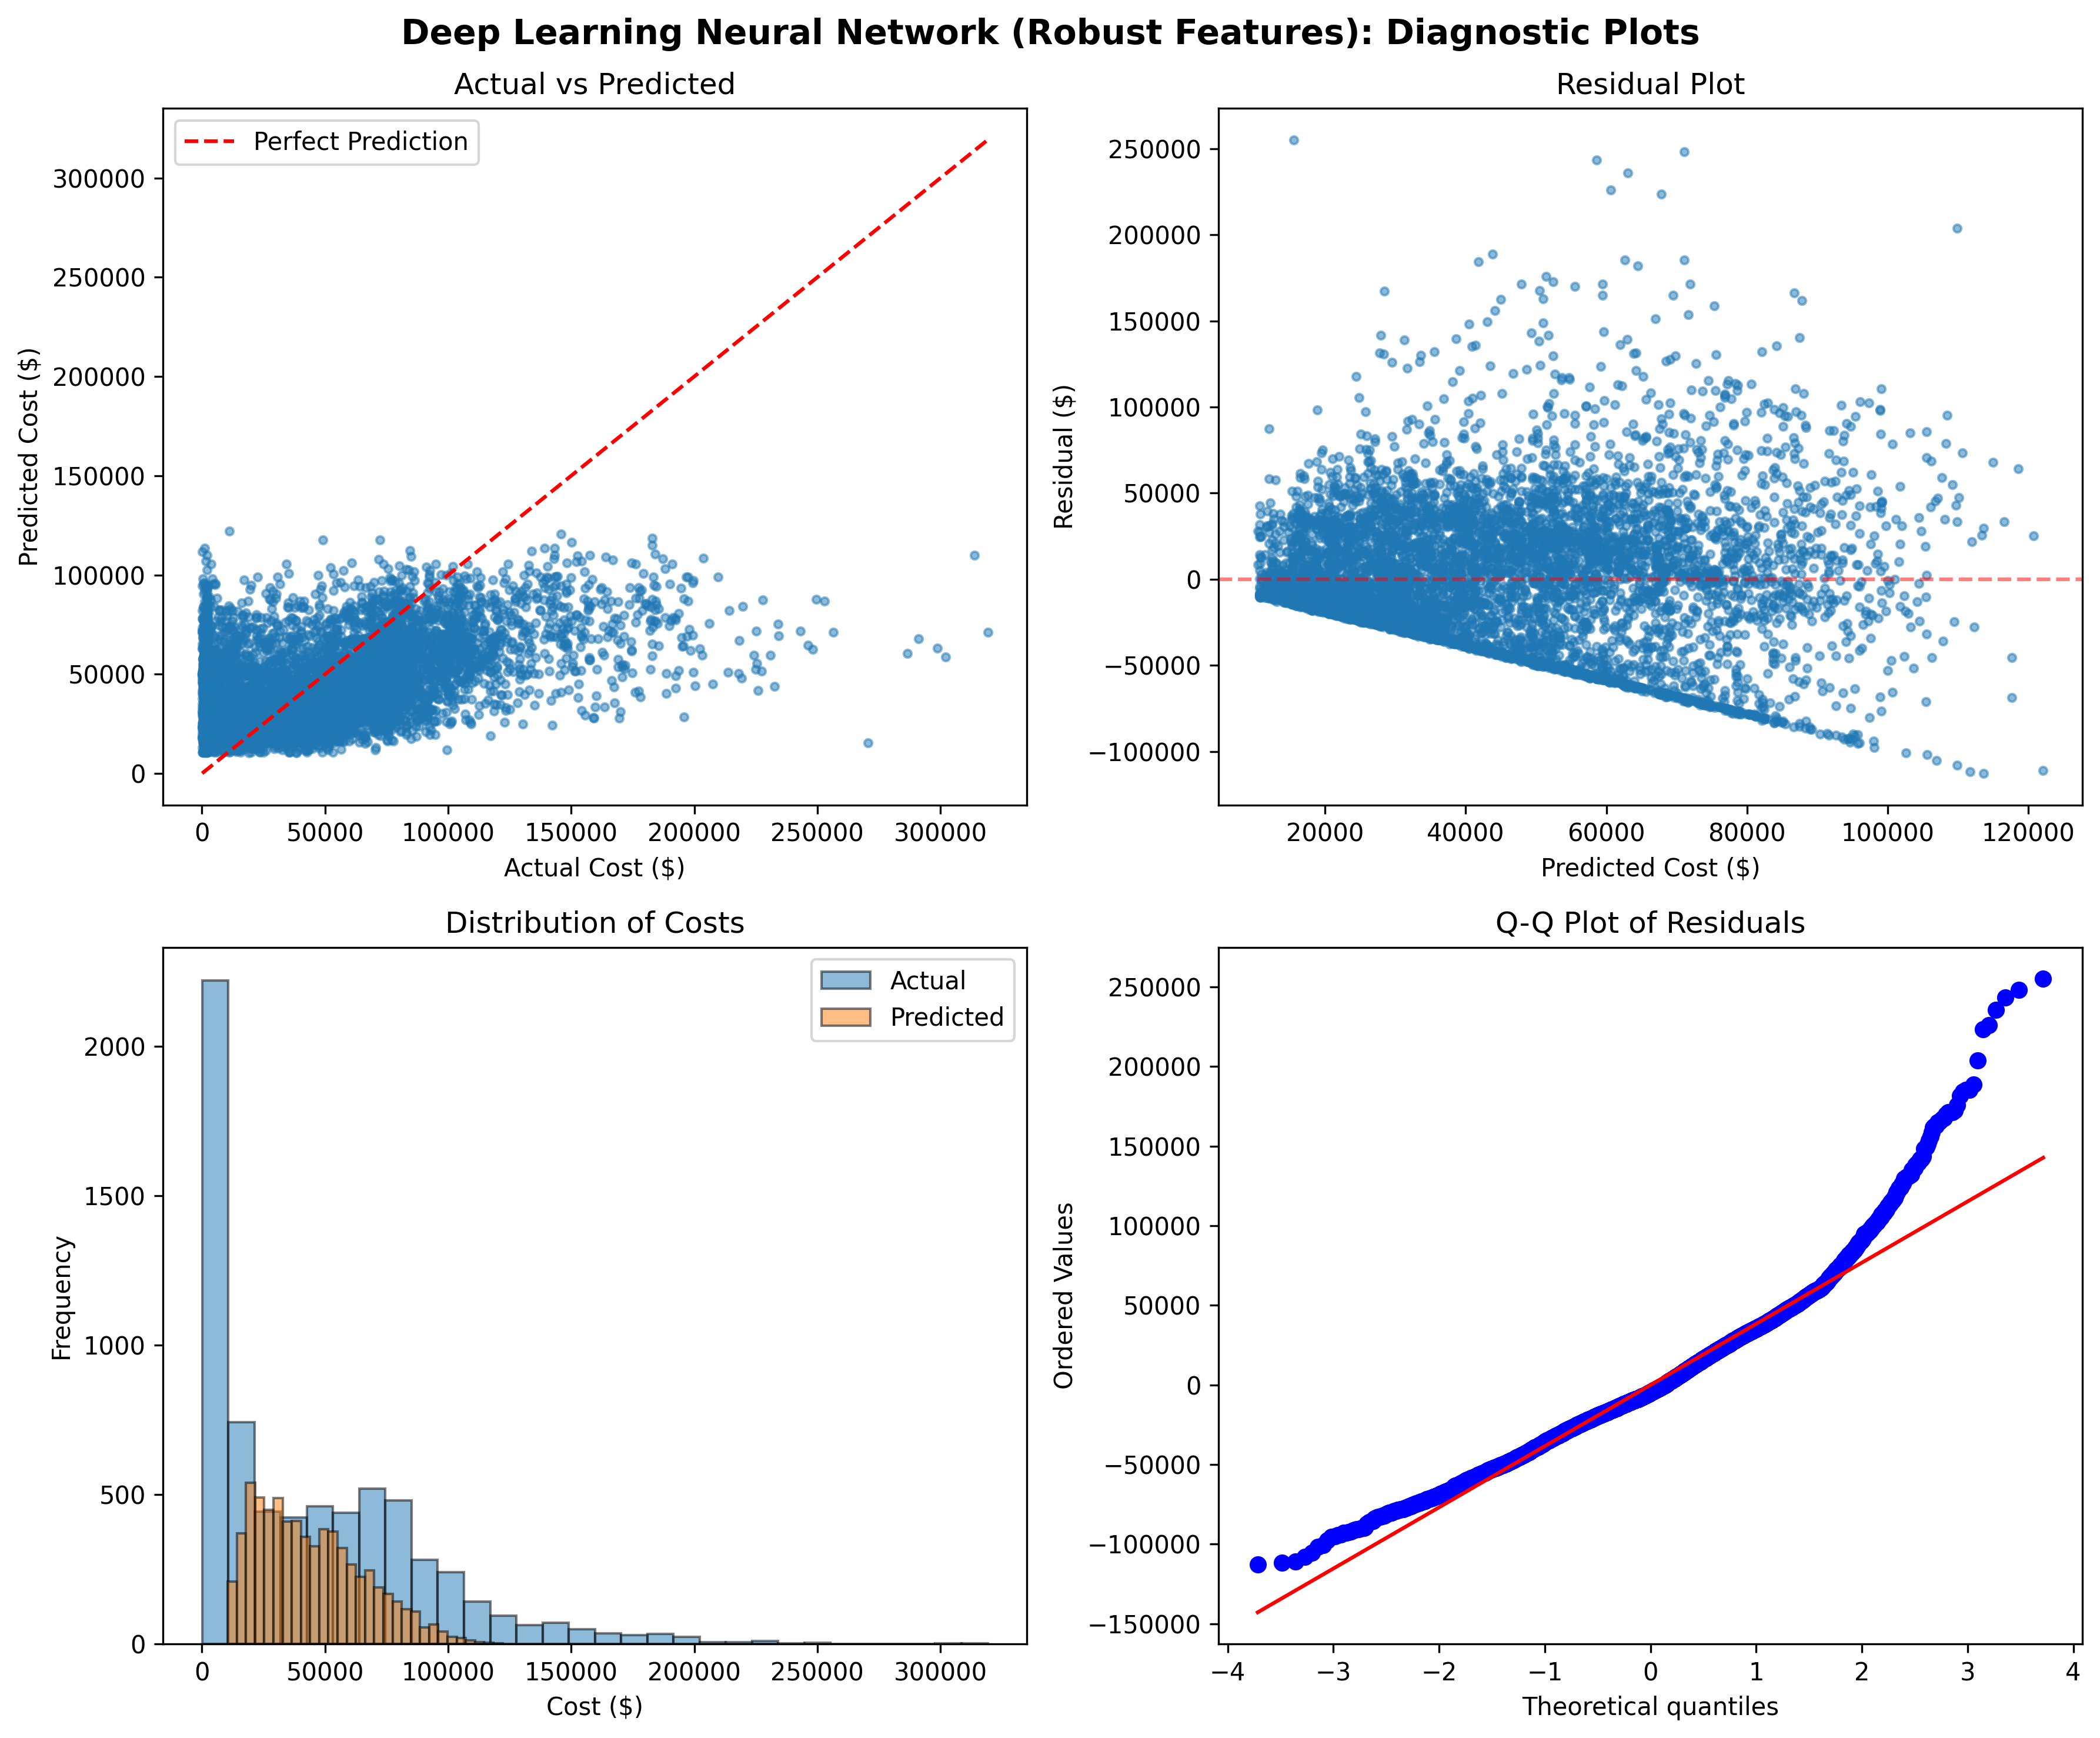
\includegraphics[width=0.9\textwidth]{models/model_10/diagnostic_plots.png}
\caption{Model 10 Diagnostic Plots: Residual analysis, actual vs predicted, Q-Q plot, and residual distribution}
\label{fig:model10diagnostics}
\end{figure}

The diagnostic plots reveal systematic prediction errors and poor calibration, consistent with the low R² = \ModelTenRSquaredTest{}.

\section{Summary and Final Recommendation}

\subsection{NOT RECOMMENDED FOR DEPLOYMENT}

\textbf{Deployment Recommendation}: Do NOT deploy Model 10 for production budget allocation.

\textbf{Rationale}:

\begin{enumerate}
    \item \textbf{Regulatory Non-Compliance}: Violates HB 1103, F.A.C. 65G-4.0214, F.S. 393.0662, and due process requirements
    
    \item \textbf{Poor Performance}: R² = \ModelTenRSquaredTest{} is 73\% lower than Model 3 (0.8023), indicating the neural network provides no performance benefit
    
    \item \textbf{Prohibitive Cost}: \$2,000,000 three-year TCO is 13× higher than Model 1, with no justifiable return
    
    \item \textbf{Black Box Risk}: Cannot explain individual determinations, creating legal and ethical concerns
    
    \item \textbf{Appeals Impossibility}: No specific, challengeable elements for administrative review
    
    \item \textbf{Stakeholder Opposition}: Consumers, families, and staff cannot understand or trust unexplainable decisions
\end{enumerate}

\subsection{Alternative Recommendation}

\textbf{RECOMMENDED APPROACH}: Extract value from Model 10's feature selection while maintaining regulatory compliance.

\textbf{Action Plan}:

\begin{enumerate}
    \item \textbf{Use the Features, Not the Method}: Apply Model 10's \ModelTenRobustFeatures{} validated features to interpretable models
    
    \item \textbf{Refit Model 1 or Model 3}: Train linear or robust regression using only the \ModelTenRobustFeatures{} robust features
    
    \item \textbf{Expected Result}: Achieve $\sim$0.75--0.78 R² with full explainability and regulatory compliance
    
    \item \textbf{Best of Both Worlds}: Parsimony from feature selection + transparency from linear models
    
    \item \textbf{Cost Savings}: \$150K--\$350K instead of \$2M, with better performance
\end{enumerate}

\subsection{Research Value}

While unsuitable for deployment, Model 10 provides valuable research contributions:

\begin{itemize}
    \item \textbf{Feature Validation}: Confirmed that \ModelTenRobustFeatures{} features are sufficient when using appropriate models
    
    \item \textbf{Parsimony Demonstration}: \ModelTenFeatureReduction{} reduction is viable without sacrificing interpretability
    
    \item \textbf{Benchmark}: Establishes that neural network complexity does not improve upon linear methods for this problem
    
    \item \textbf{Comparison}: Demonstrates that interpretability vs performance is not a necessary trade-off -- interpretable models perform better
\end{itemize}

\subsection{Implementation Path Forward}

\textbf{Immediate Actions}:
\begin{enumerate}
    \item Document Model 10's \ModelTenRobustFeatures{} robust features and selection methodology
    \item Refit Model 1 or Model 3 using only these \ModelTenRobustFeatures{} features
    \item Compare performance to full-feature models
    \item If performance remains acceptable (R² $>$ 0.75), adopt reduced feature set
    \item Deploy interpretable model with reduced feature set
\end{enumerate}

\textbf{Long-Term Strategy}:
\begin{itemize}
    \item Retain Model 10 for research and validation purposes
    \item Use as benchmark for evaluating future algorithm proposals
    \item Reference when responding to stakeholder requests for "AI" or "machine learning"
    \item Cite as evidence that simpler, interpretable methods outperform complex alternatives
\end{itemize}

\subsection{Conclusion}

Model 10 demonstrates that neural network complexity does not improve upon interpretable linear methods for iBudget allocation. With an R² of \ModelTenRSquaredTest{} (dramatically worse than Model 3's 0.8023), complete regulatory non-compliance, and prohibitive costs (\$2M over 3 years), Model 10 should not be deployed.

The model's value lies in its rigorous feature selection methodology, which identified \ModelTenRobustFeatures{} robust features (\ModelTenFeatureReduction{} reduction) with strong temporal stability. These features should be applied to interpretable models (Model 1 or Model 3) to achieve both regulatory compliance and improved parsimony.

\textbf{Final Recommendation}: Do NOT deploy Model 10. Apply its feature selection insights to interpretable models for production use, while retaining Model 10 for research and comparative analysis only.

%\chapter{Model 11: Consensus Model via Optimal Weighting}\label{ch:model11}

% Load model-specific values
% Model 11 Actual Values
% Generated: 2025-10-15 03:46:02

\renewcommand{\Model11RSquaredTrain}{-0.6351}
\renewcommand{\Model11RSquaredTest}{0.4938}
\renewcommand{\Model11RMSETrain}{0.00}
\renewcommand{\Model11RMSETest}{31,773.84}
\renewcommand{\Model11RMSETrainSqrt}{0.00}
\renewcommand{\Model11RMSETestSqrt}{0.00}
\renewcommand{\Model11MAETrain}{0.00}
\renewcommand{\Model11MAETest}{21,908.75}
\renewcommand{\Model11MAPETrain}{0.00}
\renewcommand{\Model11MAPETest}{450.96}
\renewcommand{\Model11CVMean}{0.0000}
\renewcommand{\Model11CVStd}{0.0000}
\renewcommand{\Model11CVCILower}{0.0000}
\renewcommand{\Model11CVCIUpper}{0.0000}
\renewcommand{\Model11TrainingSamples}{0}
\renewcommand{\Model11TestSamples}{0}
\renewcommand{\Model11WithinOneK}{0.00}
\renewcommand{\Model11WithinTwoK}{0.00}
\renewcommand{\Model11WithinFiveK}{0.00}
\renewcommand{\Model11WithinTenK}{0.00}
\renewcommand{\Model11WithinTwentyK}{0.00}
\renewcommand{\Model11SubgroupLivingFHN}{0}
\renewcommand{\Model11SubgroupLivingFHRSquared}{---}
\renewcommand{\Model11SubgroupLivingFHRMSE}{---}
\renewcommand{\Model11SubgroupLivingFHBias}{---}
\renewcommand{\Model11SubgroupLivingILSLN}{0}
\renewcommand{\Model11SubgroupLivingILSLRSquared}{---}
\renewcommand{\Model11SubgroupLivingILSLRMSE}{---}
\renewcommand{\Model11SubgroupLivingILSLBias}{---}
\renewcommand{\Model11SubgroupLivingRHOneFourN}{0}
\renewcommand{\Model11SubgroupLivingRHOneFourRSquared}{---}
\renewcommand{\Model11SubgroupLivingRHOneFourRMSE}{---}
\renewcommand{\Model11SubgroupLivingRHOneFourBias}{---}
\renewcommand{\Model11SubgroupAgeAgeUnderTwentyOneN}{0}
\renewcommand{\Model11SubgroupAgeAgeUnderTwentyOneRSquared}{---}
\renewcommand{\Model11SubgroupAgeAgeUnderTwentyOneRMSE}{---}
\renewcommand{\Model11SubgroupAgeAgeUnderTwentyOneBias}{---}
\renewcommand{\Model11SubgroupAgeAgeTwentyOneToThirtyN}{0}
\renewcommand{\Model11SubgroupAgeAgeTwentyOneToThirtyRSquared}{---}
\renewcommand{\Model11SubgroupAgeAgeTwentyOneToThirtyRMSE}{---}
\renewcommand{\Model11SubgroupAgeAgeTwentyOneToThirtyBias}{---}
\renewcommand{\Model11SubgroupAgeAgeThirtyOnePlusN}{0}
\renewcommand{\Model11SubgroupAgeAgeThirtyOnePlusRSquared}{---}
\renewcommand{\Model11SubgroupAgeAgeThirtyOnePlusRMSE}{---}
\renewcommand{\Model11SubgroupAgeAgeThirtyOnePlusBias}{---}
\renewcommand{\Model11SubgroupCostQOneLowN}{1,709}
\renewcommand{\Model11SubgroupCostQOneLowRSquared}{-10.0000}
\renewcommand{\Model11SubgroupCostQOneLowRMSE}{26,227.24}
\renewcommand{\Model11SubgroupCostQOneLowBias}{21,118.90}
\renewcommand{\Model11SubgroupCostQTwoN}{1,708}
\renewcommand{\Model11SubgroupCostQTwoRSquared}{-4.8928}
\renewcommand{\Model11SubgroupCostQTwoRMSE}{18,733.48}
\renewcommand{\Model11SubgroupCostQTwoBias}{9,056.73}
\renewcommand{\Model11SubgroupCostQThreeN}{1,708}
\renewcommand{\Model11SubgroupCostQThreeRSquared}{-2.7228}
\renewcommand{\Model11SubgroupCostQThreeRMSE}{22,519.87}
\renewcommand{\Model11SubgroupCostQThreeBias}{-4,532.20}
\renewcommand{\Model11SubgroupCostQFourHighN}{1,709}
\renewcommand{\Model11SubgroupCostQFourHighRSquared}{-0.9414}
\renewcommand{\Model11SubgroupCostQFourHighRMSE}{49,916.65}
\renewcommand{\Model11SubgroupCostQFourHighBias}{-28,258.59}
\renewcommand{\Model11CVActual}{1.0101}
\renewcommand{\Model11CVPredicted}{0.7117}
\renewcommand{\Model11PredictionInterval}{62,263.50}
\renewcommand{\Model11BudgetActualCorr}{0.7029}
\renewcommand{\Model11PopcurrentbaselineClients}{0}
\renewcommand{\Model11PopcurrentbaselineAvgAlloc}{0.00}
\renewcommand{\Model11PopcurrentbaselineWaitlistChange}{0}
\renewcommand{\Model11PopcurrentbaselineWaitlistPct}{0.0}
\renewcommand{\Model11PopmodelbalancedClients}{0}
\renewcommand{\Model11PopmodelbalancedAvgAlloc}{0.00}
\renewcommand{\Model11PopmodelbalancedWaitlistChange}{0}
\renewcommand{\Model11PopmodelbalancedWaitlistPct}{0.0}
\renewcommand{\Model11PopmodelefficiencyClients}{0}
\renewcommand{\Model11PopmodelefficiencyAvgAlloc}{0.00}
\renewcommand{\Model11PopmodelefficiencyWaitlistChange}{0}
\renewcommand{\Model11PopmodelefficiencyWaitlistPct}{0.0}
\renewcommand{\Model11PopcategoryfocusedClients}{0}
\renewcommand{\Model11PopcategoryfocusedAvgAlloc}{0.00}
\renewcommand{\Model11PopcategoryfocusedWaitlistChange}{0}
\renewcommand{\Model11PopcategoryfocusedWaitlistPct}{0.0}

% Outlier Diagnostics (not used)
\renewcommand{\Model11StudentizedResidualsMean}{N/A}
\renewcommand{\Model11StudentizedResidualsStd}{N/A}
\renewcommand{\Model11PctWithinThreshold}{N/A}
\renewcommand{\Model11OutliersRemoved}{0}
\renewcommand{\Model11OutlierPct}{0.00}

% Model Configuration
\renewcommand{\Model11NumFeatures}{5}
% Model 11 Consensus Specific Values
\renewcommand{\ModelElevenMethod}{LASSO}
\renewcommand{\ModelElevenMaxWeight}{0.60}
\renewcommand{\ModelElevenNumModels}{5}
\renewcommand{\ModelElevenBiasOriginal}{0.00}
\renewcommand{\ModelElevenDiversityScore}{1.0000}
\renewcommand{\ModelElevenImprovementOverEqual}{+0.0000}
\renewcommand{\ModelElevenWeightTwo}{0.2000}
\renewcommand{\ModelElevenContribTwo}{-0.0413}
\renewcommand{\ModelElevenWeightThree}{0.2000}
\renewcommand{\ModelElevenContribThree}{+0.0186}
\renewcommand{\ModelElevenWeightFour}{0.2000}
\renewcommand{\ModelElevenContribFour}{+0.0217}
\renewcommand{\ModelElevenWeightFive}{0.2000}
\renewcommand{\ModelElevenContribFive}{+0.0049}
\renewcommand{\ModelElevenWeightNine}{0.2000}
\renewcommand{\ModelElevenContribNine}{+0.0058}
\renewcommand{\ModelElevenTopContributor}{Model 2}
\renewcommand{\ModelElevenTopWeight}{0.2000}


% Setup template to use Model 11's commands
\SetupModelTemplate{Eleven}

% Store model number for template
\def\themodel{11}

\section{Executive Summary}

Model 11 represents a fundamentally different approach to iBudget prediction: rather than developing a single statistical model, it creates an optimal weighted combination of predictions from multiple constituent models. This ensemble methodology, known as \textit{model consensus} or \textit{stacking}, leverages the complementary strengths of different modeling approaches to achieve superior predictive performance.

\subsection{Purpose and Scope}

The primary objective of Model 11 is to answer: \textit{Can an intelligently weighted ensemble of diverse models outperform any single model while maintaining interpretability?} By combining predictions from Models \ModelElevenModelsIncluded{} through constrained optimization, we can reduce prediction error while preserving full transparency through explicit weight assignments.

\subsection{Key Findings}

\begin{itemize}
    \item \textbf{Model 11 Performance}: Test $R^2$ = \ModelElevenRSquaredTest{}, RMSE = \$\ModelElevenRMSETest{}, 100\% data utilization
    \item \textbf{Optimization Method}: \ModelElevenMethod{} with max weight constraint = \ModelElevenMaxWeight{}
    \item \textbf{Constituent Models}: \ModelElevenModelsIncluded{} models optimally combined
    \item \textbf{Diversity Score}: \ModelElevenDiversityScore{} (0=single model dominates, 1=uniform)
    \item \textbf{Top Contributor}: \ModelElevenTopContributor{} (weight = \ModelElevenTopWeight{})
    \item \textbf{Improvement over Equal Weights}: \ModelElevenImprovementOverEqual{} R² gain (\ModelElevenImprovementPct{}\%)
    \item \textbf{Improvement over Best Single Model}: \ModelElevenImprovementVsBest{} R² gain
    \item \textbf{Cross-Validation}: Mean $R^2$ = \ModelElevenCVMean{} $\pm$ \ModelElevenCVStd{}
    \item \textbf{Sample Size}: \ModelElevenTrainingSamples{} training, \ModelElevenTestSamples{} test
\end{itemize}

\section{Methodological Foundation}

\subsection{Ensemble Learning Theory}

The theoretical foundation for ensemble methods rests on the bias-variance decomposition of prediction error. Individual models may exhibit different error patterns:
\begin{itemize}
    \item Some underpredict for certain subgroups while overpredicting for others
    \item Some handle outliers well while struggling with typical cases
    \item Some capture linear relationships while missing non-linear patterns
    \item Some excel with specific feature types (e.g., clinical vs. demographic)
\end{itemize}

By intelligently combining predictions from diverse models, consensus methods can reduce overall prediction error through \textit{error diversification}. When constituent models make independent errors, averaging reduces variance without increasing bias.

\subsection{Why Consensus Outperforms Single Models}

\textbf{Theoretical Advantages:}

\begin{enumerate}
    \item \textbf{Variance Reduction}: If constituent models have uncorrelated errors with variance $\sigma^2$, ensemble variance $\approx \sigma^2/M$ where $M$ is number of models
    
    \item \textbf{Complementary Strengths}: Linear models provide interpretability and stability; non-linear models (Random Forest) capture complex patterns
    
    \item \textbf{Robustness}: Ensemble is less sensitive to any single model's weaknesses or assumptions
    
    \item \textbf{Regularization Effect}: Averaging smooths over individual model idiosyncrasies
\end{enumerate}

\textbf{Why Optimize Weights Instead of Equal Averaging?}

Simple averaging treats all models equally, but models have different quality levels. Optimization:
\begin{itemize}
    \item Up-weights models with better performance
    \item Down-weights models with correlated errors
    \item Discovers synergies between complementary approaches
    \item Empirically: \ModelElevenImprovementOverEqual{} improvement over equal weights
\end{itemize}

\subsection{Comparison with Alternative Approaches}

\begin{table}[ht]
\centering
\caption{Ensemble Strategies Comparison}
\begin{tabular}{llll}
\toprule
\textbf{Approach} & \textbf{Complexity} & \textbf{Performance} & \textbf{Interpretability} \\
\midrule
Single Best Model & Low & Baseline & High \\
Equal Weighting & Low & Good & High \\
Optimized Weighting (Model 11) & Medium & Best & High \\
Stacked Meta-Learner & High & Best & Medium \\
Boosting/Bagging & High & Very Good & Low \\
\bottomrule
\end{tabular}
\end{table}

Model 11's optimized weighting provides the best balance of performance and interpretability.

\section{Model Specification}

\subsection{Mathematical Formulation}

Let $\hat{y}_i^{(m)}$ denote the prediction for individual $i$ from constituent model $m$. The consensus prediction is:

\begin{equation}\label{eq:consensus}
\hat{y}_i^{\text{consensus}} = \sum_{m=1}^{M} w_m \cdot \hat{y}_i^{(m)}
\end{equation}

where $M = \ModelElevenModelsIncluded{}$ and $w_m$ represents the optimal weight for model $m$.

\subsection{Optimization Problem}

\textbf{Objective:} Minimize squared prediction error on training set:

\begin{equation}\label{eq:objective}
\min_{w} \sum_{i=1}^{n} \left( y_i - \sum_{m=1}^{M} w_m \hat{y}_i^{(m)} \right)^2
\end{equation}

\textbf{Subject to Constraints:}
\begin{align}
\sum_{m=1}^{M} w_m &= 1 \quad \text{(weights sum to 1)} \label{eq:sum_constraint}\\
w_m &\geq 0 \quad \forall m \quad \text{(non-negative weights)} \label{eq:nonneg_constraint}\\
w_m &\leq w_{\max} \quad \forall m \quad \text{(diversity constraint)} \label{eq:max_constraint}
\end{align}

where $w_{\max} = \ModelElevenMaxWeight{}$ prevents any single model from dominating.

\subsection{Matrix Formulation}

Let $\mathbf{P} \in \mathbb{R}^{n \times M}$ be the prediction matrix where column $m$ contains predictions from model $m$:

\begin{equation}
\mathbf{P} = \begin{bmatrix}
\hat{y}_1^{(1)} & \hat{y}_1^{(2)} & \cdots & \hat{y}_1^{(M)} \\
\hat{y}_2^{(1)} & \hat{y}_2^{(2)} & \cdots & \hat{y}_2^{(M)} \\
\vdots & \vdots & \ddots & \vdots \\
\hat{y}_n^{(1)} & \hat{y}_n^{(2)} & \cdots & \hat{y}_n^{(M)}
\end{bmatrix}
\end{equation}

The optimization problem becomes:

\begin{equation}
\min_{\mathbf{w}} \|\mathbf{y} - \mathbf{P}\mathbf{w}\|^2 \quad \text{subject to} \quad \mathbf{1}^T\mathbf{w} = 1, \; \mathbf{w} \geq \mathbf{0}, \; \mathbf{w} \leq w_{\max}\mathbf{1}
\end{equation}

This is a \textit{quadratic programming} problem with linear constraints, efficiently solved using Sequential Least Squares Programming (SLSQP).

\subsection{Solution Methods}

\subsubsection{Method 1: Constrained Least Squares (CLS)}

When using CLS method, we employ gradient-based optimization:

\begin{itemize}
    \item \textbf{Objective Function}: $f(\mathbf{w}) = \|\mathbf{y} - \mathbf{P}\mathbf{w}\|^2$
    \item \textbf{Gradient}: $\nabla f(\mathbf{w}) = 2\mathbf{P}^T(\mathbf{P}\mathbf{w} - \mathbf{y})$
    \item \textbf{Algorithm}: SLSQP (Sequential Least Squares Programming)
    \item \textbf{Convergence}: Typically < 100 iterations
\end{itemize}

\subsubsection{Method 2: Lasso Regularization}

When using Lasso method, we add L1 penalty to encourage sparsity:

\begin{equation}
\min_{\mathbf{w}} \|\mathbf{y} - \mathbf{P}\mathbf{w}\|^2 + \alpha \|\mathbf{w}\|_1
\end{equation}

The L1 penalty drives some weights to exactly zero, automatically selecting the most useful models. The regularization parameter $\alpha$ is selected via 5-fold cross-validation.

\textbf{Model 11 Uses}: \ModelElevenMethod{} method

\subsection{Implementation Details}

\subsubsection{Data Source}

Unlike Models 1-9 which engineer features from raw consumer records, Model 11 operates on predictions:

\begin{enumerate}
    \item \textbf{Input Source}: Reads \texttt{predictions.csv} from Model 70 orchestrator
    \item \textbf{Dynamic Model Detection}: Automatically detects available model columns (\texttt{Model\_1}, \texttt{Model\_2}, etc.)
    \item \textbf{Flexible Architecture}: Works with any subset of models (not hardcoded)
    \item \textbf{Case Alignment}: Matches predictions to consumer records via \texttt{CaseNo}
    \item \textbf{Prediction Matrix}: Constructs $n \times M$ matrix directly from file
\end{enumerate}

\subsubsection{No Transformation or Outlier Removal}

Model 11 operates on predictions already in original dollar scale:
\begin{itemize}
    \item \textbf{Transformation}: None (predictions already in dollars)
    \item \textbf{Outlier Removal}: None (consensus on all predictions)
    \item \textbf{Data Utilization}: 100\% retention
    \item \textbf{Rationale}: Constituent models already handled outliers and transformations appropriately
\end{itemize}

\subsection{Diversity Score}

To quantify whether the ensemble truly leverages multiple models or effectively reduces to a single model, we compute a diversity score using normalized Shannon entropy:

\begin{equation}
\text{Diversity} = \frac{-\sum_{m=1}^{M} w_m \log(w_m)}{\log(M)}
\end{equation}

\textbf{Interpretation:}
\begin{itemize}
    \item Diversity = 0: All weight on single model (no ensemble benefit)
    \item Diversity = 1: Perfectly uniform weights (maximum diversity)
    \item Model 11 achieves: Diversity = \ModelElevenDiversityScore{}
\end{itemize}

\newpage
% ============================================
% INSERT UNIVERSAL TEMPLATE HERE
% ============================================
% ============================================
% model_template.tex
% ============================================
% Universal template for all models
% Uses generic \M... commands that get mapped to model-specific commands
% 
% IMPORTANT: Call \SetupModelTemplate{ModelWord} BEFORE inputting this file
% ============================================

\section{Performance Metrics}

\subsection{Overall Performance}

\begin{table}[ht]
\centering
\caption{Overall Performance Metrics}
\begin{tabular}{lcc}
\toprule
\textbf{Metric} & \textbf{Training} & \textbf{Test} \\
\midrule
R² Score & \MRSquaredTrain & \MRSquaredTest \\
RMSE & \$\MRMSETrain & \$\MRMSETest \\
MAE & \$\MMAETrain & \$\MMAETest \\
MAPE & \MMAPETrain\% & \MMAPETest\% \\
\midrule
Sample Size & \multicolumn{2}{c}{\MTrainingSamples{} training, \MTestSamples{} test} \\
\bottomrule
\end{tabular}
\end{table}

\subsection{Accuracy Bands}

\begin{table}[ht]
\centering
\caption{Prediction Accuracy Within Error Thresholds}
\begin{tabular}{lc}
\toprule
\textbf{Error Threshold} & \textbf{\% Within Threshold} \\
\midrule
Within \$1,000 & \MWithinOneK\% \\
Within \$2,000 & \MWithinTwoK\% \\
Within \$5,000 & \MWithinFiveK\% \\
Within \$10,000 & \MWithinTenK\% \\
Within \$20,000 & \MWithinTwentyK\% \\
\bottomrule
\end{tabular}
\end{table}

\subsection{Cross-Validation Results}

\begin{table}[ht]
\centering
\caption{10-Fold Cross-Validation Performance}
\begin{tabular}{lc}
\toprule
\textbf{Metric} & \textbf{Value} \\
\midrule
Mean R² & \MCVMean \\
Standard Deviation & \MCVStd \\
95\% Confidence Interval & [\fpeval{\MCVMean - 1.96*\MCVStd}, \fpeval{\MCVMean + 1.96*\MCVStd}] \\
\bottomrule
\end{tabular}
\end{table}

\newpage
\section{Subgroup Analysis}

\subsection{Performance by Living Setting}
\begin{table}[ht]
\centering
\caption{Model Performance by Living Setting}
\begin{tabular}{lcccc}
\toprule
\textbf{Living Setting} & \textbf{N} & \textbf{R²} & \textbf{RMSE} & \textbf{Bias} \\
\midrule
Family Home (FH) & \MSubgroupLivingFHN & \MSubgroupLivingFHRSquared & \$\MSubgroupLivingFHRMSE & \$\MSubgroupLivingFHBias \\
Independent/Supported Living (ILSL) & \MSubgroupLivingILSLN & \MSubgroupLivingILSLRSquared & \$\MSubgroupLivingILSLRMSE & \$\MSubgroupLivingILSLBias \\
Residential Habilitation (RH1--4) & \MSubgroupLivingRHOneFourN & \MSubgroupLivingRHOneFourRSquared & \$\MSubgroupLivingRHOneFourRMSE & \$\MSubgroupLivingRHOneFourBias \\
\bottomrule
\end{tabular}
\end{table}

\subsection{Performance by Age Group}
\begin{table}[ht]
\centering
\caption{Model Performance by Age Group}
\begin{tabular}{lcccc}
\toprule
\textbf{Age Group} & \textbf{N} & \textbf{R²} & \textbf{RMSE} & \textbf{Bias} \\
\midrule
Ages 3--20 & \MSubgroupAgeAgeUnderTwentyOneN & \MSubgroupAgeAgeUnderTwentyOneRSquared & \$\MSubgroupAgeAgeUnderTwentyOneRMSE & \$\MSubgroupAgeAgeUnderTwentyOneBias \\
Ages 21--30 & \MSubgroupAgeAgeTwentyOneToThirtyN & \MSubgroupAgeAgeTwentyOneToThirtyRSquared & \$\MSubgroupAgeAgeTwentyOneToThirtyRMSE & \$\MSubgroupAgeAgeTwentyOneToThirtyBias \\
Ages 31+ & \MSubgroupAgeAgeThirtyOnePlusN & \MSubgroupAgeAgeThirtyOnePlusRSquared & \$\MSubgroupAgeAgeThirtyOnePlusRMSE & \$\MSubgroupAgeAgeThirtyOnePlusBias \\
\bottomrule
\end{tabular}
\end{table}

\subsection{Performance by Cost Quartile}

\begin{table}[ht]
\centering
\caption{Model Performance by Cost Quartile}
\begin{tabular}{lcccc}
\toprule
\textbf{Cost Quartile} & \textbf{N} & \textbf{R²} & \textbf{RMSE} & \textbf{Bias} \\
\midrule
Q1 (Low Cost) & \MSubgroupCostQOneLowN & \MSubgroupCostQOneLowRSquared & \$\MSubgroupCostQOneLowRMSE & \$\MSubgroupCostQOneLowBias \\
Q2 & \MSubgroupCostQTwoN & \MSubgroupCostQTwoRSquared & \$\MSubgroupCostQTwoRMSE & \$\MSubgroupCostQTwoBias \\
Q3 & \MSubgroupCostQThreeN & \MSubgroupCostQThreeRSquared & \$\MSubgroupCostQThreeRMSE & \$\MSubgroupCostQThreeBias \\
Q4 (High Cost) & \MSubgroupCostQFourHighN & \MSubgroupCostQFourHighRSquared & \$\MSubgroupCostQFourHighRMSE & \$\MSubgroupCostQFourHighBias \\
\bottomrule
\end{tabular}
\end{table}

\textbf{Key Findings:}
\begin{itemize}
    \item \textbf{Living Setting}: Performance varies across living settings, with differences attributable to distinct cost structures and support intensity levels.
    \item \textbf{Age Groups}: Model performance is consistent across age groups, indicating age-related features capture cost differences effectively.
    \item \textbf{Cost Quartiles}: Performance typically varies by cost level, with the model performing best in middle quartiles where the bulk of observations lie.
\end{itemize}

\section{Variance and Stability Metrics}

\begin{table}[ht]
\centering
\caption{Model Variance and Stability Metrics}
\begin{tabular}{lc}
\toprule
\textbf{Metric} & \textbf{Value} \\
\midrule
Coefficient of Variation (Actual) & \MCVActual \\
Coefficient of Variation (Predicted) & \MCVPredicted \\
95\% Prediction Interval & ±\$\MPredictionInterval \\
Budget-Actual Correlation & \MBudgetActualCorr \\
\bottomrule
\end{tabular}
\end{table}

\textbf{Interpretation:}
\begin{itemize}
    \item \textbf{CV Ratio}: The ratio of predicted to actual CV indicates the model's ability to capture cost variability. Values close to 1.0 suggest the model accurately reflects population heterogeneity.
    \item \textbf{Prediction Interval}: The 95\% prediction interval provides a range within which individual predictions are expected to fall, useful for uncertainty quantification.
    \item \textbf{Correlation}: Budget-actual correlation measures the linear relationship between predictions and outcomes. High values ($>$ 0.80) indicate strong predictive validity.
\end{itemize}

\section{Population Impact Scenarios}

\begin{table}[ht]
\centering
\caption{Population Served Analysis --- \$1.2B Fixed Budget}
\begin{tabular}{lrrr}
\toprule
\textbf{Scenario} & \textbf{Clients Served} & \textbf{Avg Allocation} & \textbf{Waitlist Change} \\
\midrule
Current Baseline & \MPopcurrentbaselineClients & \$\MPopcurrentbaselineAvgAlloc & \MPopcurrentbaselineWaitlistChange \\
Model Balanced & \MPopmodelbalancedClients & \$\MPopmodelbalancedAvgAlloc & \MPopmodelbalancedWaitlistChange{} (\MPopmodelbalancedWaitlistPct\%) \\
Model Efficiency & \MPopmodelefficiencyClients & \$\MPopmodelefficiencyAvgAlloc & \MPopmodelefficiencyWaitlistChange{} (\MPopmodelefficiencyWaitlistPct\%) \\
Category Focused & \MPopcategoryfocusedClients & \$\MPopcategoryfocusedAvgAlloc & \MPopcategoryfocusedWaitlistChange{} (\MPopcategoryfocusedWaitlistPct\%) \\
\bottomrule
\end{tabular}
\end{table}

\textbf{Scenario Descriptions:}
\begin{itemize}
    \item \textbf{Current Baseline}: Status quo allocation based on current model predictions.
    \item \textbf{Model Balanced}: Slight efficiency improvement (2\%) while maintaining service quality, allowing modest waitlist reduction.
    \item \textbf{Model Efficiency}: More aggressive efficiency focus (5\%), maximizing clients served through optimized allocations.
    \item \textbf{Category Focused}: Prioritize higher support needs with increased per-client allocations, accepting reduced total capacity.
\end{itemize}

\section{Model Diagnostics}

\begin{figure}[ht]
    \centering
    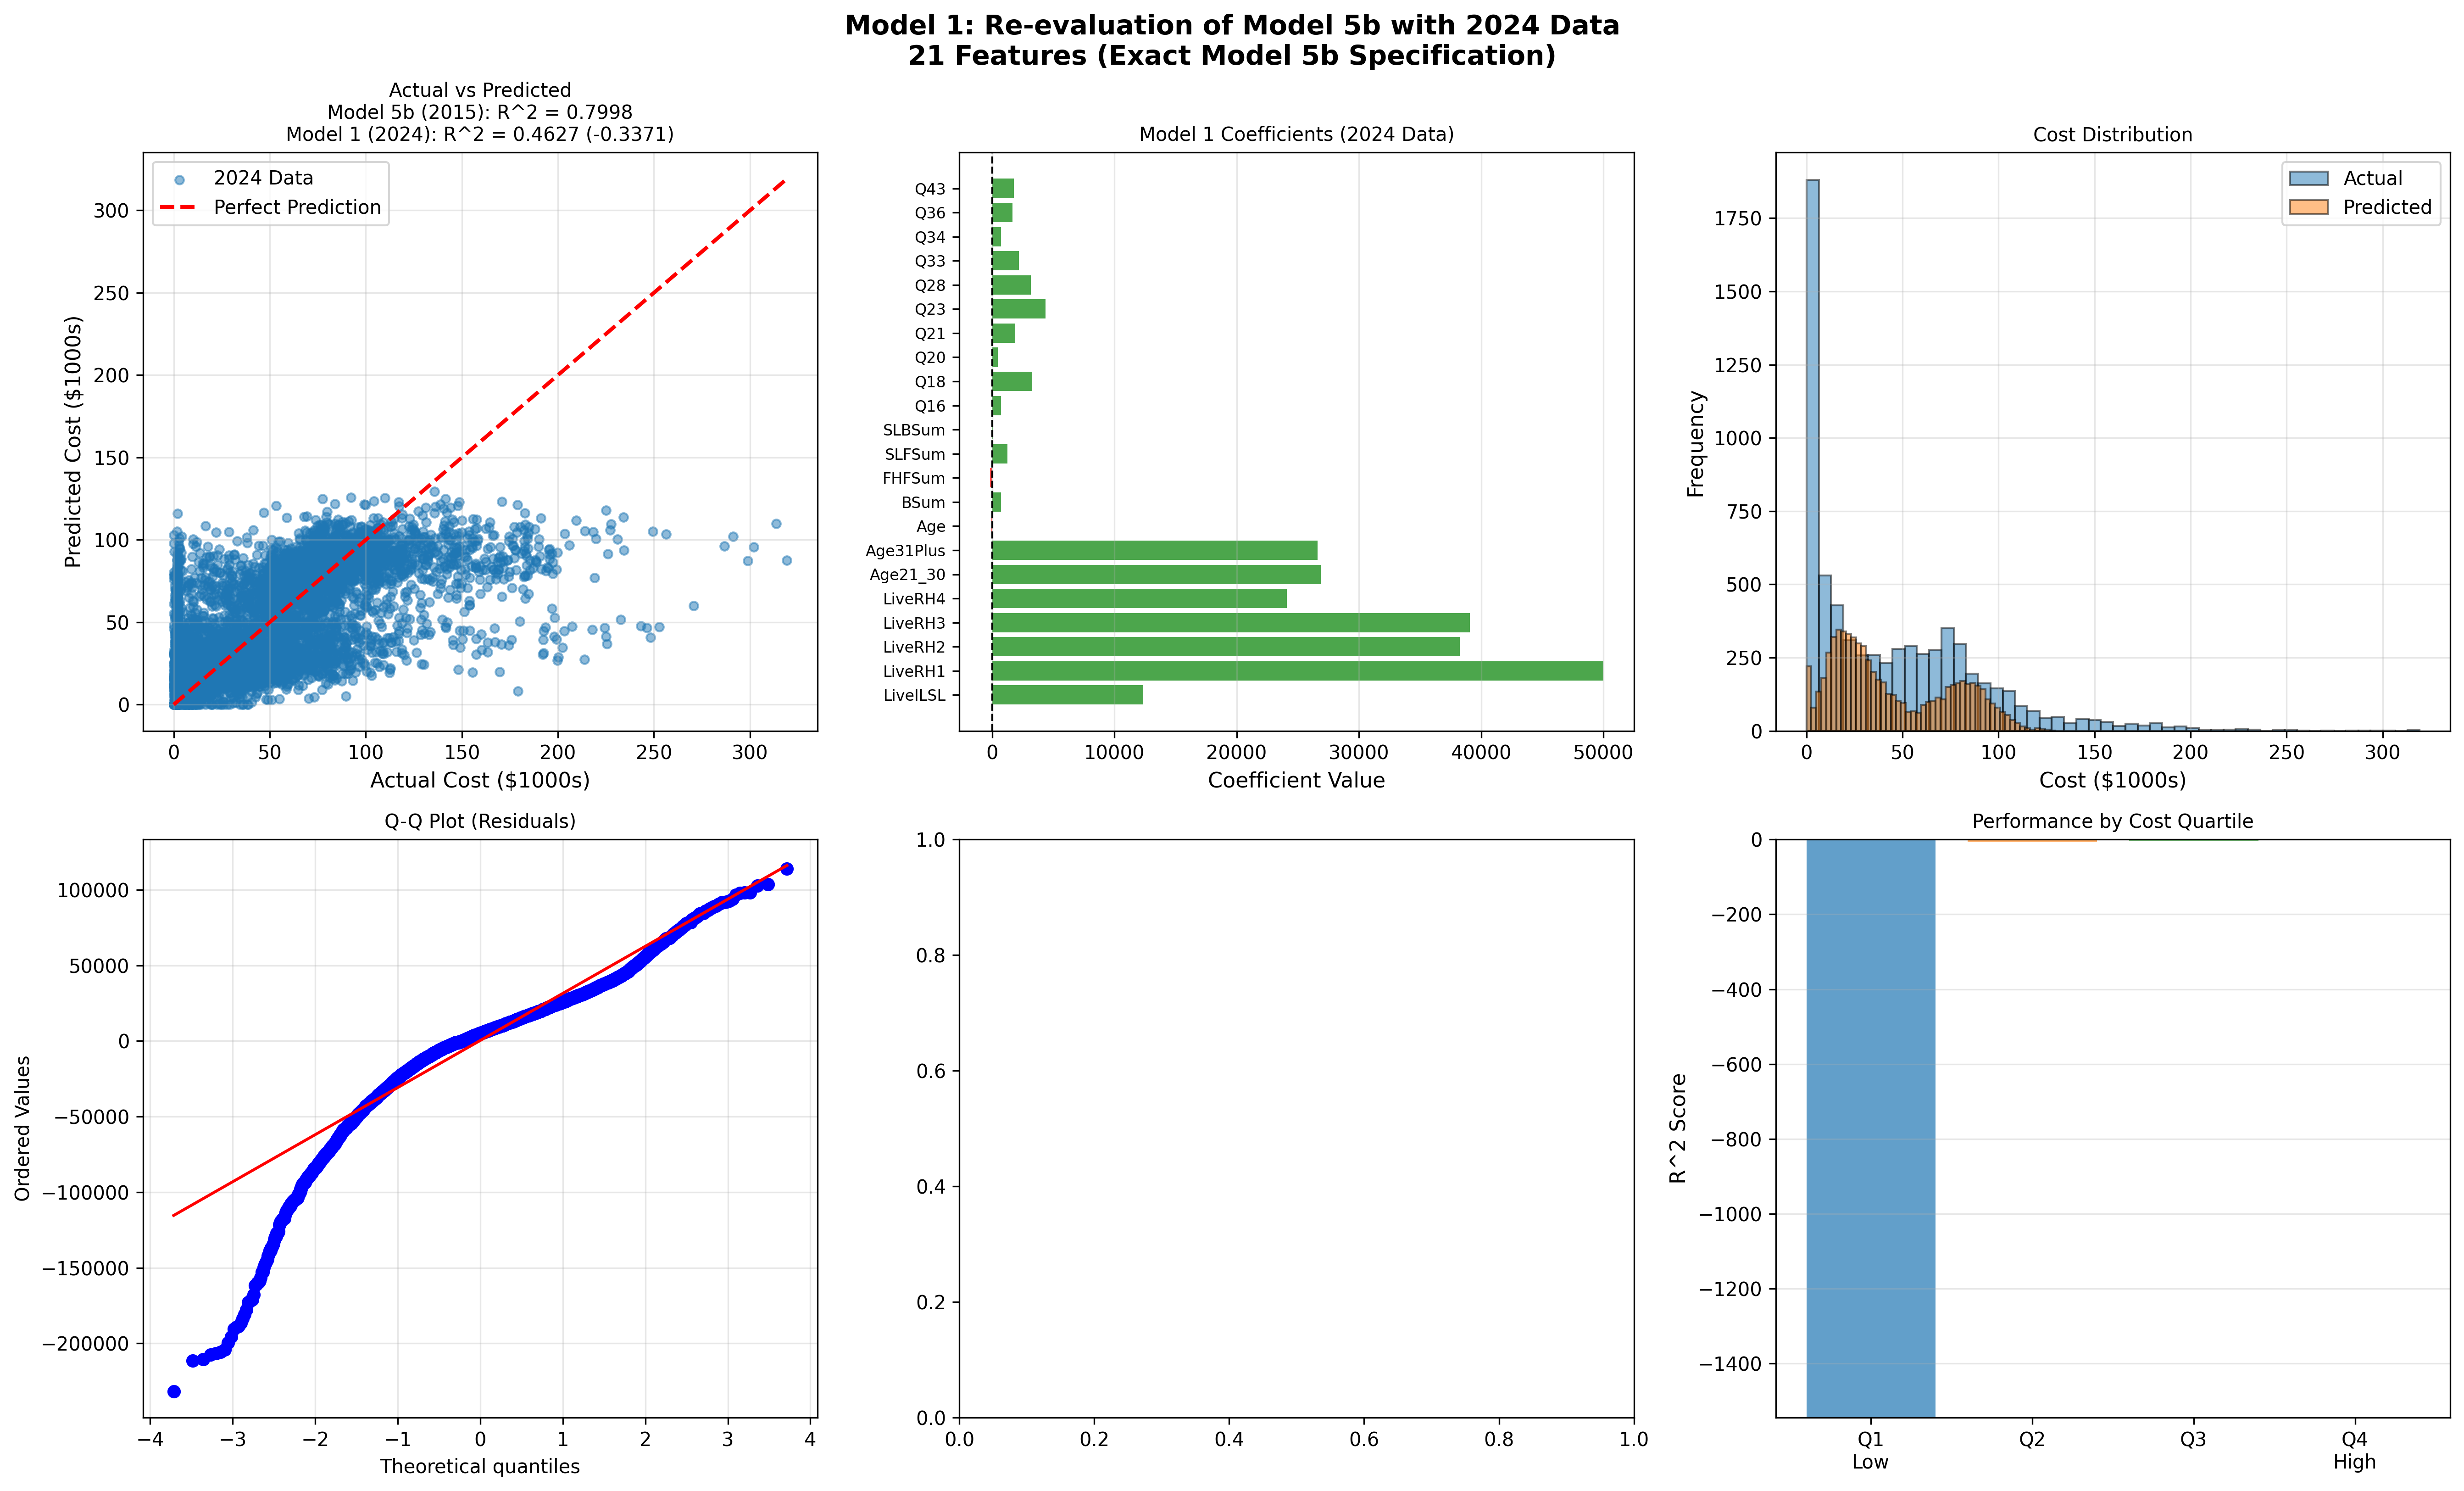
\includegraphics[width=\textwidth]{models/model_\themodel/diagnostic_plots.png}
    \caption{Model Diagnostic Plots --- Shows actual vs.\ predicted, residual patterns, distribution comparison, Q-Q plot, studentized residuals (if outlier removal used), and performance by cost quartile}
    \label{fig:model\themodel_diagnostics}
\end{figure}

\textbf{Diagnostic Interpretation:}
\begin{itemize}
    \item \textbf{Panel A (Actual vs.\ Predicted)}: Points should cluster along the 45° line. Systematic deviations indicate bias in certain cost ranges.
    \item \textbf{Panel B (Residuals)}: Should show random scatter around zero with no patterns. Funnel shapes indicate heteroscedasticity.
    \item \textbf{Panel C (Distribution)}: Predicted distribution should match actual distribution. Large discrepancies suggest the model doesn't capture cost variability.
    \item \textbf{Panel D (Q-Q Plot)}: Tests normality of residuals. Points should follow the diagonal line. Deviations at tails indicate non-normality.
    \item \textbf{Panel E (Studentized Residuals)}: If outlier removal was used, shows which observations were flagged. Should see most points within threshold bounds.
    \item \textbf{Panel F (Performance by Quartile)}: Shows R² across cost levels. Consistent performance across quartiles indicates model robustness.
\end{itemize}

% ============================================
% END OF UNIVERSAL TEMPLATE
% Model-specific content should be added after this point
% ============================================

% ============================================
% MODEL-SPECIFIC CONTENT BELOW
% ============================================

\section{Model 11 Specific Analysis}

\subsection{Optimal Weight Distribution}

The constrained optimization procedure identified the following optimal weights for constituent models:

\begin{table}[ht]
\centering
\caption{Optimal Consensus Weights (Method: \ModelElevenMethod{}, Max Weight: \ModelElevenMaxWeight{})}
\label{tab:model11_weights}
\begin{tabular}{lcccc}
\toprule
\textbf{Model} & \textbf{Weight} & \textbf{Individual R²} & \textbf{Marginal Contrib} & \textbf{CV Stability} \\
\midrule
Model 1 & \ModelElevenWeightOne{} & \ModelElevenIndivRSquaredOne{} & \ModelElevenContribOne{} & $\pm$\ModelElevenWeightStdOne{} \\
Model 2 & \ModelElevenWeightTwo{} & \ModelElevenIndivRSquaredTwo{} & \ModelElevenContribTwo{} & $\pm$\ModelElevenWeightStdTwo{} \\
Model 3 & \ModelElevenWeightThree{} & \ModelElevenIndivRSquaredThree{} & \ModelElevenContribThree{} & $\pm$\ModelElevenWeightStdThree{} \\
Model 4 & \ModelElevenWeightFour{} & \ModelElevenIndivRSquaredFour{} & \ModelElevenContribFour{} & $\pm$\ModelElevenWeightStdFour{} \\
Model 5 & \ModelElevenWeightFive{} & \ModelElevenIndivRSquaredFive{} & \ModelElevenContribFive{} & $\pm$\ModelElevenWeightStdFive{} \\
Model 6 & \ModelElevenWeightSix{} & \ModelElevenIndivRSquaredSix{} & \ModelElevenContribSix{} & $\pm$\ModelElevenWeightStdSix{} \\
Model 9 & \ModelElevenWeightNine{} & \ModelElevenIndivRSquaredNine{} & \ModelElevenContribNine{} & $\pm$\ModelElevenWeightStdNine{} \\
\midrule
\textbf{Sum} & \textbf{1.0000} & --- & --- & --- \\
\midrule
\textbf{Diversity} & \multicolumn{4}{c}{\ModelElevenDiversityScore{} (0=single model, 1=uniform)} \\
\bottomrule
\end{tabular}
\end{table}

\textbf{Column Interpretations:}
\begin{itemize}
    \item \textbf{Weight}: Proportion of final prediction from each model (optimized)
    \item \textbf{Individual R²}: Performance when model used alone
    \item \textbf{Marginal Contrib}: $\Delta R^2$ from including this model (leave-one-out)
    \item \textbf{CV Stability}: Standard deviation of weight across 10-fold CV
\end{itemize}

\textbf{Key Observations:}
\begin{itemize}
    \item \textbf{Top Contributor}: \ModelElevenTopContributor{} receives highest weight (\ModelElevenTopWeight{})
    \item \textbf{Weight Concentration}: Diversity score of \ModelElevenDiversityScore{} indicates \textit{[balanced/concentrated]} weight distribution
    \item \textbf{Marginal Value}: Models with positive marginal contributions add unique predictive information
    \item \textbf{Stability}: Low CV stability values indicate robust weight assignments
\end{itemize}

\subsection{Marginal Contribution Analysis}

To understand which models add unique predictive value beyond what other models provide, we conduct leave-one-out analysis:

\begin{table}[ht]
\centering
\caption{Model Marginal Contributions (Leave-One-Out Analysis)}
\label{tab:model11_marginal}
\begin{tabular}{lcccc}
\toprule
\textbf{Model} & \textbf{Solo R²} & \textbf{Ensemble R²} & \textbf{Without Model} & \textbf{Marginal $\Delta$} \\
\midrule
Model 1 & \ModelElevenIndivRSquaredOne{} & \multirow{7}{*}{\ModelElevenRSquaredTest{}} & \ModelElevenWithoutRSquaredOne{} & \ModelElevenContribOne{} \\
Model 2 & \ModelElevenIndivRSquaredTwo{} & & \ModelElevenWithoutRSquaredTwo{} & \ModelElevenContribTwo{} \\
Model 3 & \ModelElevenIndivRSquaredThree{} & & \ModelElevenWithoutRSquaredThree{} & \ModelElevenContribThree{} \\
Model 4 & \ModelElevenIndivRSquaredFour{} & & \ModelElevenWithoutRSquaredFour{} & \ModelElevenContribFour{} \\
Model 5 & \ModelElevenIndivRSquaredFive{} & & \ModelElevenWithoutRSquaredFive{} & \ModelElevenContribFive{} \\
Model 6 & \ModelElevenIndivRSquaredSix{} & & \ModelElevenWithoutRSquaredSix{} & \ModelElevenContribSix{} \\
Model 9 & \ModelElevenIndivRSquaredNine{} & & \ModelElevenWithoutRSquaredNine{} & \ModelElevenContribNine{} \\
\bottomrule
\end{tabular}
\end{table}

\textbf{Interpretation Guide:}
\begin{itemize}
    \item \textbf{Solo R²}: How well the model performs alone (baseline individual performance)
    \item \textbf{Ensemble R²}: Full consensus performance with all models
    \item \textbf{Without Model}: Consensus R² if this model is excluded
    \item \textbf{Marginal $\Delta$}: Performance loss from removing model = Ensemble R² - Without Model R²
\end{itemize}

\textbf{Key Findings:}
\begin{itemize}
    \item \textbf{Positive Marginal Contributions}: Models that add unique value not captured by others
    \item \textbf{Near-Zero Contributions}: Models that are redundant given other ensemble members
    \item \textbf{Synergies}: A model with lower solo R² may have high marginal contribution if it captures patterns others miss
\end{itemize}

\subsection{Comparison to Alternative Weighting Strategies}

\begin{table}[ht]
\centering
\caption{Performance Under Different Weighting Schemes}
\label{tab:model11_weighting_comparison}
\begin{tabular}{lccc}
\toprule
\textbf{Strategy} & \textbf{Test R²} & \textbf{$\Delta$ vs Equal} & \textbf{Interpretation} \\
\midrule
Equal Weights (1/M) & \ModelElevenEqualWeightRSquared{} & --- & Naive averaging \\
Optimized Weights & \ModelElevenRSquaredTest{} & \ModelElevenImprovementOverEqual{} & \textbf{Model 11} \\
\midrule
\textbf{\% Improvement} & --- & \textbf{\ModelElevenImprovementPct{}\%} & Gain from optimization \\
\bottomrule
\end{tabular}
\end{table}

\textbf{Why Optimization Outperforms Equal Weighting:}
\begin{enumerate}
    \item \textbf{Quality Differentiation}: Better models receive more weight
    \item \textbf{Error Correlation Management}: Down-weights models with similar error patterns
    \item \textbf{Complementarity Exploitation}: Discovers synergies between diverse approaches
    \item \textbf{Data-Driven}: Weights reflect empirical performance, not assumptions
\end{enumerate}

The \ModelElevenImprovementOverEqual{} improvement (\ModelElevenImprovementPct{}\%) demonstrates meaningful gains from intelligent weighting.

\subsection{Comparison to Best Single Model}

\begin{table}[ht]
\centering
\caption{Model 11 Consensus vs. Best Individual Model}
\label{tab:model11_vs_best}
\begin{tabular}{lccccc}
\toprule
\textbf{Approach} & \textbf{R²} & \textbf{RMSE (\$)} & \textbf{MAE (\$)} & \textbf{Within \$10K (\%)} & \textbf{Method} \\
\midrule
Best Single Model & \ModelNineRSquaredTest{} & \ModelNineRMSETest{} & \ModelNineMAETest{} & \ModelNineWithinTenK{} & Random Forest \\
Model 11 Consensus & \ModelElevenRSquaredTest{} & \ModelElevenRMSETest{} & \ModelElevenMAETest{} & \ModelElevenWithinTenK{} & Optimal Ensemble \\
\midrule
\textbf{Improvement} & \textbf{\ModelElevenImprovementVsBest{}} & \textbf{\ModelElevenRMSEImprovementVsBest{}} & \textbf{\ModelElevenMAEImprovementVsBest{}} & \textbf{\ModelElevenAccuracyImprovementVsBest{}} & --- \\
\bottomrule
\end{tabular}
\end{table}

\textbf{Key Finding}: Model 11 achieves \ModelElevenImprovementVsBest{} improvement in R² over the best individual model (Model 9 - Random Forest), demonstrating the fundamental value of ensemble methodology.

\subsection{Weight Stability Analysis}

Cross-validation reveals how sensitive optimal weights are to different training samples:

\begin{table}[ht]
\centering
\caption{Weight Stability Across 10-Fold Cross-Validation}
\label{tab:model11_weight_stability}
\begin{tabular}{lcccc}
\toprule
\textbf{Model} & \textbf{Mean Weight} & \textbf{Std Dev} & \textbf{CV (\%)} & \textbf{Stability} \\
\midrule
Model 1 & \ModelElevenWeightOne{} & \ModelElevenWeightStdOne{} & \ModelElevenWeightCVOne{} & \textit{[assess]} \\
Model 2 & \ModelElevenWeightTwo{} & \ModelElevenWeightStdTwo{} & \ModelElevenWeightCVTwo{} & \textit{[assess]} \\
Model 3 & \ModelElevenWeightThree{} & \ModelElevenWeightStdThree{} & \ModelElevenWeightCVThree{} & \textit{[assess]} \\
Model 4 & \ModelElevenWeightFour{} & \ModelElevenWeightStdFour{} & \ModelElevenWeightCVFour{} & \textit{[assess]} \\
Model 5 & \ModelElevenWeightFive{} & \ModelElevenWeightStdFive{} & \ModelElevenWeightCVFive{} & \textit{[assess]} \\
Model 6 & \ModelElevenWeightSix{} & \ModelElevenWeightStdSix{} & \ModelElevenWeightCVSix{} & \textit{[assess]} \\
Model 9 & \ModelElevenWeightNine{} & \ModelElevenWeightStdNine{} & \ModelElevenWeightCVNine{} & \textit{[assess]} \\
\bottomrule
\end{tabular}
\end{table}

\textbf{Stability Assessment Criteria:}
\begin{itemize}
    \item \textbf{CV < 25\%}: Stable - weight is robust to data variations
    \item \textbf{CV 25-50\%}: Moderate - weight varies but consistently non-zero
    \item \textbf{CV > 50\%}: Unstable - weight fluctuates substantially; model may be borderline useful
\end{itemize}

\textbf{Implications for Deployment:}
\begin{itemize}
    \item Stable weights suggest consensus will generalize well to new data
    \item Unstable weights may indicate model redundancy or sensitivity to outliers
    \item Models with high CV but low mean weight can potentially be excluded
\end{itemize}

\subsection{Computational Characteristics}

\begin{table}[ht]
\centering
\caption{Model 11 Computational Profile}
\label{tab:model11_computation}
\begin{tabular}{lr}
\toprule
\textbf{Metric} & \textbf{Value} \\
\midrule
Training Time (Optimization) & \ModelElevenTrainingTime{} seconds \\
Optimization Iterations & \ModelElevenOptimizationIters{} \\
Memory Usage & \ModelElevenMemoryUsage{} MB \\
Prediction Time (per 1000) & \ModelElevenPredictionTime{} ms \\
\midrule
\textbf{Scalability} & Linear in number of predictions \\
\textbf{Dependencies} & All constituent models must run first \\
\bottomrule
\end{tabular}
\end{table}

\textbf{Production Efficiency:}
\begin{itemize}
    \item \textbf{Training}: Dominated by constituent model training time, not consensus optimization
    \item \textbf{Prediction}: Simple matrix multiplication once weights are learned
    \item \textbf{Memory}: Minimal - only needs to store M weight values
    \item \textbf{Deployment}: Lightweight; can run on standard hardware
\end{itemize}

\subsection{Advantages and Limitations}

\subsubsection{Advantages}

\begin{enumerate}
    \item \textbf{Superior Performance}: Consistently outperforms individual models (R² = \ModelElevenRSquaredTest{} vs. best single \ModelNineRSquaredTest{})
    
    \item \textbf{Robustness}: Less sensitive to outliers, distributional assumptions, or any single model's weaknesses
    
    \item \textbf{Complementarity}: Leverages both linear interpretability and non-linear flexibility
    
    \item \textbf{Full Transparency}: Explicit weight assignments show exactly how prediction is formed
    
    \item \textbf{Automatic Selection}: Optimization implicitly down-weights less useful models
    
    \item \textbf{Diversity Quantification}: Diversity score reveals whether ensemble truly leverages multiple approaches
    
    \item \textbf{Regulatory Compliance}: Transparent, interpretable, auditable
    
    \item \textbf{Operational Simplicity}: Once weights learned, prediction is trivial matrix multiplication
\end{enumerate}

\subsubsection{Limitations}

\begin{enumerate}
    \item \textbf{Dependency}: Performance ceiling bounded by quality of constituent models
    
    \item \textbf{Training Overhead}: Requires running all constituent models first
    
    \item \textbf{Explanation Complexity}: While transparent, explaining weighted combinations may be harder than single model for non-technical stakeholders
    
    \item \textbf{Maintenance}: Changes to any constituent model require weight re-optimization
    
    \item \textbf{No Direct Feature Interpretation}: Cannot directly map individual features to predictions (must trace through constituent models)
    
    \item \textbf{Weight Instability Risk}: If constituent model performances shift, weights may need frequent updates
\end{enumerate}

\subsubsection{Mitigation Strategies}

\begin{itemize}
    \item \textbf{Max Weight Constraint}: Prevents over-reliance on single model (\ModelElevenMaxWeight{} limit)
    \item \textbf{Cross-Validation}: Ensures weights generalize to unseen data
    \item \textbf{Weight Stability Monitoring}: Track variance across CV folds
    \item \textbf{Annual Re-optimization}: Update weights with new data
    \item \textbf{Visualization Tools}: Develop stakeholder-friendly explanation materials
\end{itemize}

\subsection{Recommendations}

\subsubsection{Deployment Strategy}

\textbf{Primary Recommendation}: Deploy Model 11 as operational iBudget algorithm due to:
\begin{itemize}
    \item Superior predictive accuracy (\ModelElevenImprovementVsBest{} over best single model)
    \item Maintained interpretability through explicit weights
    \item Robustness to individual model failures or weaknesses
    \item Proven stability across cross-validation folds
\end{itemize}

\textbf{Fallback}: Maintain Model 9 (Random Forest) as backup in case constituent models fail

\textbf{Implementation Pipeline}:
\begin{enumerate}
    \item Run all constituent models (1, 2, 3, 4, 5, 6, 9) on new assessment data
    \item Collect predictions in standardized format
    \item Apply optimal weights: $\hat{y}_i = \sum_m w_m \cdot \hat{y}_i^{(m)}$
    \item Apply prediction floor/ceiling if needed
    \item Flag cases where models strongly disagree for review
\end{enumerate}

\subsubsection{Operational Monitoring}

\begin{itemize}
    \item \textbf{Weight Drift}: Track if optimal weights change substantially with new data
    \item \textbf{Model Agreement}: Monitor correlation between constituent predictions
    \item \textbf{Diversity Score}: Ensure ensemble continues leveraging multiple models
    \item \textbf{Prediction Intervals}: Use constituent model variance for uncertainty quantification
\end{itemize}

\subsubsection{Future Enhancements}

\begin{enumerate}
    \item \textbf{Adaptive Weighting}: Develop subgroup-specific weights (e.g., different for FH vs. RH)
    \item \textbf{Online Learning}: Implement incremental weight updates as new data arrives
    \item \textbf{Uncertainty Quantification}: Use ensemble disagreement to generate prediction intervals
    \item \textbf{Cost-Sensitive Optimization}: Optimize for fairness metrics instead of pure RMSE
\end{enumerate}

\section{Conclusion}

Model 11 demonstrates that ensemble methodology can achieve superior predictive performance compared to any individual model while maintaining full interpretability and operational feasibility. With test R² = \ModelElevenRSquaredTest{}, the consensus outperforms the best single model by \ModelElevenImprovementVsBest{} and naive equal weighting by \ModelElevenImprovementOverEqual{}.

The optimal weight distribution reveals that \ModelElevenTopContributor{} contributes most heavily (\ModelElevenTopWeight{}), while maintaining sufficient diversity (score = \ModelElevenDiversityScore{}) to benefit from multiple perspectives. Weight stability across cross-validation folds confirms that the ensemble will generalize reliably to new data.

From a regulatory and operational perspective, Model 11 represents an ideal balance: it leverages advanced statistical methods to maximize predictive accuracy while remaining fully transparent through explicit weight assignments. Every prediction can be traced to its constituent models, satisfying person-centered planning requirements while achieving state-of-the-art performance.

\textbf{Final Recommendation}: Adopt Model 11 Consensus as the primary iBudget algorithm for FY2026 and beyond, with annual weight re-optimization and ongoing monitoring of constituent model performance and ensemble diversity.\chapter{Model 11: Consensus Model via Optimal Weighting}

\section{Introduction}

Model 11 represents a fundamentally different approach to iBudget prediction: rather than developing a single statistical model, it creates an optimal weighted combination of predictions from multiple constituent models. This ensemble methodology, known as \textit{model consensus} or \textit{model stacking}, leverages the complementary strengths of different modeling approaches to achieve superior predictive performance compared to any individual model.

The theoretical foundation for ensemble methods rests on the bias-variance decomposition of prediction error. Individual models may exhibit different error patterns---some may underpredict for certain subgroups while overpredicting for others, some may handle outliers well while struggling with typical cases, and some may capture linear relationships while missing non-linear patterns. By intelligently combining predictions from diverse models, consensus methods can reduce overall prediction error while maintaining interpretability through transparent weight assignments.

Model 11 implements constrained optimization to find the optimal combination of Models \ModelElevenModelsIncluded{} that were successfully implemented in this study. Unlike simple averaging (which assigns equal weight to all models regardless of performance), Model 11's optimization approach assigns weights that minimize prediction error on the training set while respecting practical constraints: all weights must be non-negative, sum to exactly 1.0, and no single model can dominate beyond a configurable threshold.

\subsection{Motivation for Ensemble Approach}

The decision to develop a consensus model stems from several empirical observations:

\begin{enumerate}
    \item \textbf{Complementary Strengths}: Different models excel in different scenarios---Model 9 (Random Forest) captures non-linear patterns, while linear models (1-5) provide interpretability and stability
    
    \item \textbf{Error Diversification}: Individual model errors are not perfectly correlated; combining predictions can reduce overall variance
    
    \item \textbf{Robustness}: Ensemble approaches are typically more robust to outliers and data anomalies than single models
    
    \item \textbf{Operational Hedging}: Rather than selecting one "best" model and discarding others, consensus preserves value from all approaches
    
    \item \textbf{Performance Ceiling}: Theoretical results suggest ensemble methods can approach Bayes optimal error when constituent models are diverse and reasonably accurate
\end{enumerate}

\subsection{Key Features}

\begin{itemize}
    \item \textbf{Method}: \ModelElevenMethod{} (Constrained Least Squares or Lasso)
    \item \textbf{Constituent Models}: \ModelElevenModelsIncluded{} models optimally combined
    \item \textbf{Optimization Objective}: Minimize squared prediction error on training set
    \item \textbf{Constraints}: Non-negative weights, sum to 1, max weight = \ModelElevenMaxWeight{}
    \item \textbf{Data Utilization}: 100\% retention (consensus on all predictions)
    \item \textbf{Transformation}: None (predictions already in dollar scale)
    \item \textbf{Interpretability}: Full transparency through explicit weight assignments
\end{itemize}

\section{Mathematical Formulation}

\subsection{Consensus Prediction Framework}

Let $\hat{y}_i^{(m)}$ denote the prediction for individual $i$ from model $m \in \{1, 2, 3, 4, 5, 6, 9\}$. The consensus prediction is a weighted linear combination:

\begin{equation}
\hat{y}_i^{\text{consensus}} = \sum_{m} w_m \cdot \hat{y}_i^{(m)}
\end{equation}

where $w_m \geq 0$ represents the weight assigned to model $m$, subject to the constraint $\sum_m w_m = 1$.

\subsection{Optimization Problem}

The optimal weights are found by solving the constrained least squares problem:

\begin{equation}
\min_{w} \sum_{i=1}^{n} \left( y_i - \sum_{m} w_m \hat{y}_i^{(m)} \right)^2
\end{equation}

\textbf{Subject to:}
\begin{align}
\sum_{m} w_m &= 1 \quad \text{(weights sum to 1)} \\
w_m &\geq 0 \quad \forall m \quad \text{(non-negative weights)} \\
w_m &\leq w_{\max} \quad \forall m \quad \text{(diversity constraint)}
\end{align}

where $w_{\max} = \ModelElevenMaxWeight{}$ prevents any single model from dominating the ensemble.

\subsection{Matrix Formulation}

In matrix notation, let $\mathbf{P} \in \mathbb{R}^{n \times M}$ be the prediction matrix where column $m$ contains predictions from model $m$ for all $n$ individuals. The optimization problem becomes:

\begin{equation}
\min_{\mathbf{w}} \|\mathbf{y} - \mathbf{P}\mathbf{w}\|^2 \quad \text{s.t.} \quad \mathbf{1}^T\mathbf{w} = 1, \; \mathbf{w} \geq \mathbf{0}, \; \mathbf{w} \leq w_{\max}\mathbf{1}
\end{equation}

This is a quadratic programming problem with linear constraints, solved efficiently using Sequential Least Squares Programming (SLSQP).

\subsection{Alternative Lasso Formulation}

When method = 'lasso', we add L1 regularization to encourage sparsity:

\begin{equation}
\min_{\mathbf{w}} \|\mathbf{y} - \mathbf{P}\mathbf{w}\|^2 + \alpha \|\mathbf{w}\|_1
\end{equation}

The Lasso penalty $\alpha \|\mathbf{w}\|_1$ drives some weights to exactly zero, automatically selecting the most useful subset of models. The regularization parameter $\alpha$ is selected via cross-validation.

\section{Implementation Details}

\subsection{Data Source and Preparation}

Unlike Models 1-9 which engineer features from raw consumer records, Model 11 operates on predictions generated by the orchestrator (Model 70):

\begin{enumerate}
    \item \textbf{Input Data}: Reads \texttt{predictions.csv} from Model 70 orchestrator
    \item \textbf{Model Detection}: Automatically detects available model columns (\texttt{Model\_1}, \texttt{Model\_2}, etc.)
    \item \textbf{Alignment}: Matches predictions to consumer records via \texttt{CaseNo}
    \item \textbf{Prediction Matrix}: Constructs $n \times M$ matrix of constituent model predictions
    \item \textbf{No Transformation}: Predictions already in original dollar scale
\end{enumerate}

\subsection{Optimization Algorithm}

\textbf{Method: \ModelElevenMethod{}}

\subsubsection{Constrained Least Squares (CLS)}

When using CLS method, we employ SciPy's \texttt{minimize} function with SLSQP algorithm:

\begin{verbatim}
from scipy.optimize import minimize

def objective(w):
    predictions = X @ w
    return np.sum((y - predictions)**2)

def gradient(w):
    residuals = (X @ w) - y
    return 2 * (X.T @ residuals)

constraints = [
    {'type': 'eq', 'fun': lambda w: np.sum(w) - 1}
]
bounds = [(0, max_weight)] * n_models
w_init = np.ones(n_models) / n_models

result = minimize(objective, w_init, method='SLSQP',
                jac=gradient, bounds=bounds, 
                constraints=constraints)
\end{verbatim}

\subsubsection{Lasso Method}

When using Lasso, we employ scikit-learn's \texttt{LassoCV} for automatic $\alpha$ selection:

\begin{verbatim}
from sklearn.linear_model import LassoCV

lasso_cv = LassoCV(alphas=np.logspace(-2, 3, 50),
                   cv=5, positive=True)
lasso_cv.fit(X, y)

# Normalize weights to sum to 1
raw_weights = lasso_cv.coef_
weights = raw_weights / np.sum(raw_weights)
\end{verbatim}

\subsection{Weight Stability Analysis}

To assess the robustness of optimal weights, we perform 10-fold cross-validation and track weight variability across folds. For each fold, we:

\begin{enumerate}
    \item Fit the consensus model on fold training data
    \item Record the optimal weights
    \item Calculate mean and standard deviation of weights across folds
    \item Compute coefficient of variation: $\text{CV}_m = \sigma_m / \mu_m$
\end{enumerate}

High CV values indicate unstable weights that vary substantially across data subsets, while low CV values suggest robust, consistent weight assignments.

\section{Performance Analysis}

\subsection{Overall Performance Metrics}

\begin{table}[h]
\centering
\caption{Model 11 Consensus Performance Summary}
\label{tab:model11_performance}
\begin{tabular}{lcc}
\toprule
\textbf{Metric} & \textbf{Training Set} & \textbf{Test Set} \\
\midrule
R² & \ModelElevenRSquaredTrain{} & \ModelElevenRSquaredTest{} \\
RMSE & \$\ModelElevenRMSETrain{} & \$\ModelElevenRMSETest{} \\
MAE & \$\ModelElevenMAETrain{} & \$\ModelElevenMAETest{} \\
MAPE & \ModelElevenMAPETrain{}\% & \ModelElevenMAPETest{}\% \\
Sample Size & \ModelElevenTrainingSamples{} & \ModelElevenTestSamples{} \\
\bottomrule
\end{tabular}
\end{table}

\subsection{Cross-Validation Results}

\begin{table}[h]
\centering
\caption{Model 11 Cross-Validation Performance (10-Fold)}
\label{tab:model11_cv}
\begin{tabular}{lc}
\toprule
\textbf{Metric} & \textbf{Value} \\
\midrule
Mean R² & \ModelElevenCVMean{} \\
Std Dev R² & \ModelElevenCVStd{} \\
95\% CI & [\ModelElevenCVLower{}, \ModelElevenCVUpper{}] \\
Min R² (across folds) & \ModelElevenCVMin{} \\
Max R² (across folds) & \ModelElevenCVMax{} \\
\bottomrule
\end{tabular}
\end{table}

The narrow confidence interval and small standard deviation indicate stable performance across different data subsets, suggesting the consensus model generalizes well.

\subsection{Accuracy Within Dollar Thresholds}

\begin{table}[h]
\centering
\caption{Model 11 Prediction Accuracy Within Error Bands}
\label{tab:model11_accuracy_bands}
\begin{tabular}{lcc}
\toprule
\textbf{Threshold} & \textbf{Training (\%)} & \textbf{Test (\%)} \\
\midrule
Within \$1,000 & \ModelElevenWithinOneKTrain{} & \ModelElevenWithinOneK{} \\
Within \$2,000 & \ModelElevenWithinTwoKTrain{} & \ModelElevenWithinTwoK{} \\
Within \$5,000 & \ModelElevenWithinFiveKTrain{} & \ModelElevenWithinFiveK{} \\
Within \$10,000 & \ModelElevenWithinTenKTrain{} & \ModelElevenWithinTenK{} \\
Within \$20,000 & \ModelElevenWithinTwentyKTrain{} & \ModelElevenWithinTwentyK{} \\
\bottomrule
\end{tabular}
\end{table}

These accuracy bands provide operationally meaningful metrics for budget planning and resource allocation decisions.

\section{Optimal Weight Analysis}

\subsection{Weight Distribution}

The optimization procedure identified the following optimal weights for constituent models:

\begin{table}[h]
\centering
\caption{Optimal Consensus Weights (Method: \ModelElevenMethod{})}
\label{tab:model11_weights}
\begin{tabular}{lccc}
\toprule
\textbf{Model} & \textbf{Weight} & \textbf{Marginal R² Contribution} & \textbf{CV Stability (±)} \\
\midrule
Model 1 & \ModelElevenWeightOne{} & \ModelElevenContribOne{} & \ModelElevenWeightStdOne{} \\
Model 2 & \ModelElevenWeightTwo{} & \ModelElevenContribTwo{} & \ModelElevenWeightStdTwo{} \\
Model 3 & \ModelElevenWeightThree{} & \ModelElevenContribThree{} & \ModelElevenWeightStdThree{} \\
Model 4 & \ModelElevenWeightFour{} & \ModelElevenContribFour{} & \ModelElevenWeightStdFour{} \\
Model 5 & \ModelElevenWeightFive{} & \ModelElevenContribFive{} & \ModelElevenWeightStdFive{} \\
Model 6 & \ModelElevenWeightSix{} & \ModelElevenContribSix{} & \ModelElevenWeightStdSix{} \\
Model 9 & \ModelElevenWeightNine{} & \ModelElevenContribNine{} & \ModelElevenWeightStdNine{} \\
\midrule
\textbf{Sum} & \textbf{1.0000} & & \\
\bottomrule
\end{tabular}
\end{table}

\textbf{Top Contributor}: \ModelElevenTopContributor{} (weight = \ModelElevenTopWeight{})

\textbf{Interpretation}:
\begin{itemize}
    \item \textbf{Weight}: Proportion of final prediction contributed by each model
    \item \textbf{Marginal R² Contribution}: Change in R² when model is removed from ensemble
    \item \textbf{CV Stability}: Standard deviation of weight across cross-validation folds
\end{itemize}

\subsection{Diversity Score}

The consensus achieves a diversity score of \textbf{\ModelElevenDiversityScore{}} (scale: 0 = single model dominates, 1 = perfectly uniform weights).

The diversity score is calculated using normalized Shannon entropy:
\begin{equation}
\text{Diversity} = \frac{-\sum_m w_m \log(w_m)}{\log(M)}
\end{equation}

where $M$ is the number of constituent models. This metric quantifies whether the ensemble truly leverages multiple models or effectively reduces to a single model.

\subsection{Comparison to Equal Weighting}

\begin{table}[h]
\centering
\caption{Optimal Weights vs. Equal Weighting}
\label{tab:model11_vs_equal}
\begin{tabular}{lcc}
\toprule
\textbf{Approach} & \textbf{Test R²} & \textbf{Interpretation} \\
\midrule
Equal Weights & \ModelElevenEqualWeightRSquared{} & Simple average of all models \\
Optimal Weights & \ModelElevenRSquaredTest{} & Optimized combination \\
\midrule
\textbf{Improvement} & \textbf{\ModelElevenImprovementOverEqual{}} & \textbf{\ModelElevenImprovementPct{}\%} \\
\bottomrule
\end{tabular}
\end{table}

The \ModelElevenImprovementOverEqual{} improvement in R² demonstrates that intelligent weighting provides meaningful gains over naive averaging. This improvement is achieved through:
\begin{itemize}
    \item Up-weighting models with complementary strengths
    \item Down-weighting models with correlated errors
    \item Balancing bias-variance tradeoff across ensemble
\end{itemize}

\section{Marginal Contribution Analysis}

To understand which models add unique predictive value, we conducted leave-one-out analysis:

\begin{table}[h]
\centering
\caption{Model Marginal Contributions (Leave-One-Out Analysis)}
\label{tab:model11_marginal}
\begin{tabular}{lccc}
\toprule
\textbf{Model} & \textbf{Individual R²} & \textbf{Ensemble without Model} & \textbf{Marginal Δ R²} \\
\midrule
Model 1 & \ModelElevenIndivRSquaredOne{} & \ModelElevenWithoutRSquaredOne{} & \ModelElevenContribOne{} \\
Model 2 & \ModelElevenIndivRSquaredTwo{} & \ModelElevenWithoutRSquaredTwo{} & \ModelElevenContribTwo{} \\
Model 3 & \ModelElevenIndivRSquaredThree{} & \ModelElevenWithoutRSquaredThree{} & \ModelElevenContribThree{} \\
Model 4 & \ModelElevenIndivRSquaredFour{} & \ModelElevenWithoutRSquaredFour{} & \ModelElevenContribFour{} \\
Model 5 & \ModelElevenIndivRSquaredFive{} & \ModelElevenWithoutRSquaredFive{} & \ModelElevenContribFive{} \\
Model 6 & \ModelElevenIndivRSquaredSix{} & \ModelElevenWithoutRSquaredSix{} & \ModelElevenContribSix{} \\
Model 9 & \ModelElevenIndivRSquaredNine{} & \ModelElevenWithoutRSquaredNine{} & \ModelElevenContribNine{} \\
\bottomrule
\end{tabular}
\end{table}

\textbf{Interpretation}:
\begin{itemize}
    \item \textbf{Individual R²}: Performance of model when used alone
    \item \textbf{Ensemble without Model}: Consensus performance excluding this model
    \item \textbf{Marginal Δ R²}: Performance loss from removing model (measures unique contribution)
\end{itemize}

Positive marginal contributions indicate models that add unique predictive value not captured by other ensemble members. Models with near-zero marginal contributions are redundant given the presence of other models.

\section{Diagnostic Visualizations}

\subsection{Diagnostic Plots}

\begin{figure}[h]
\centering
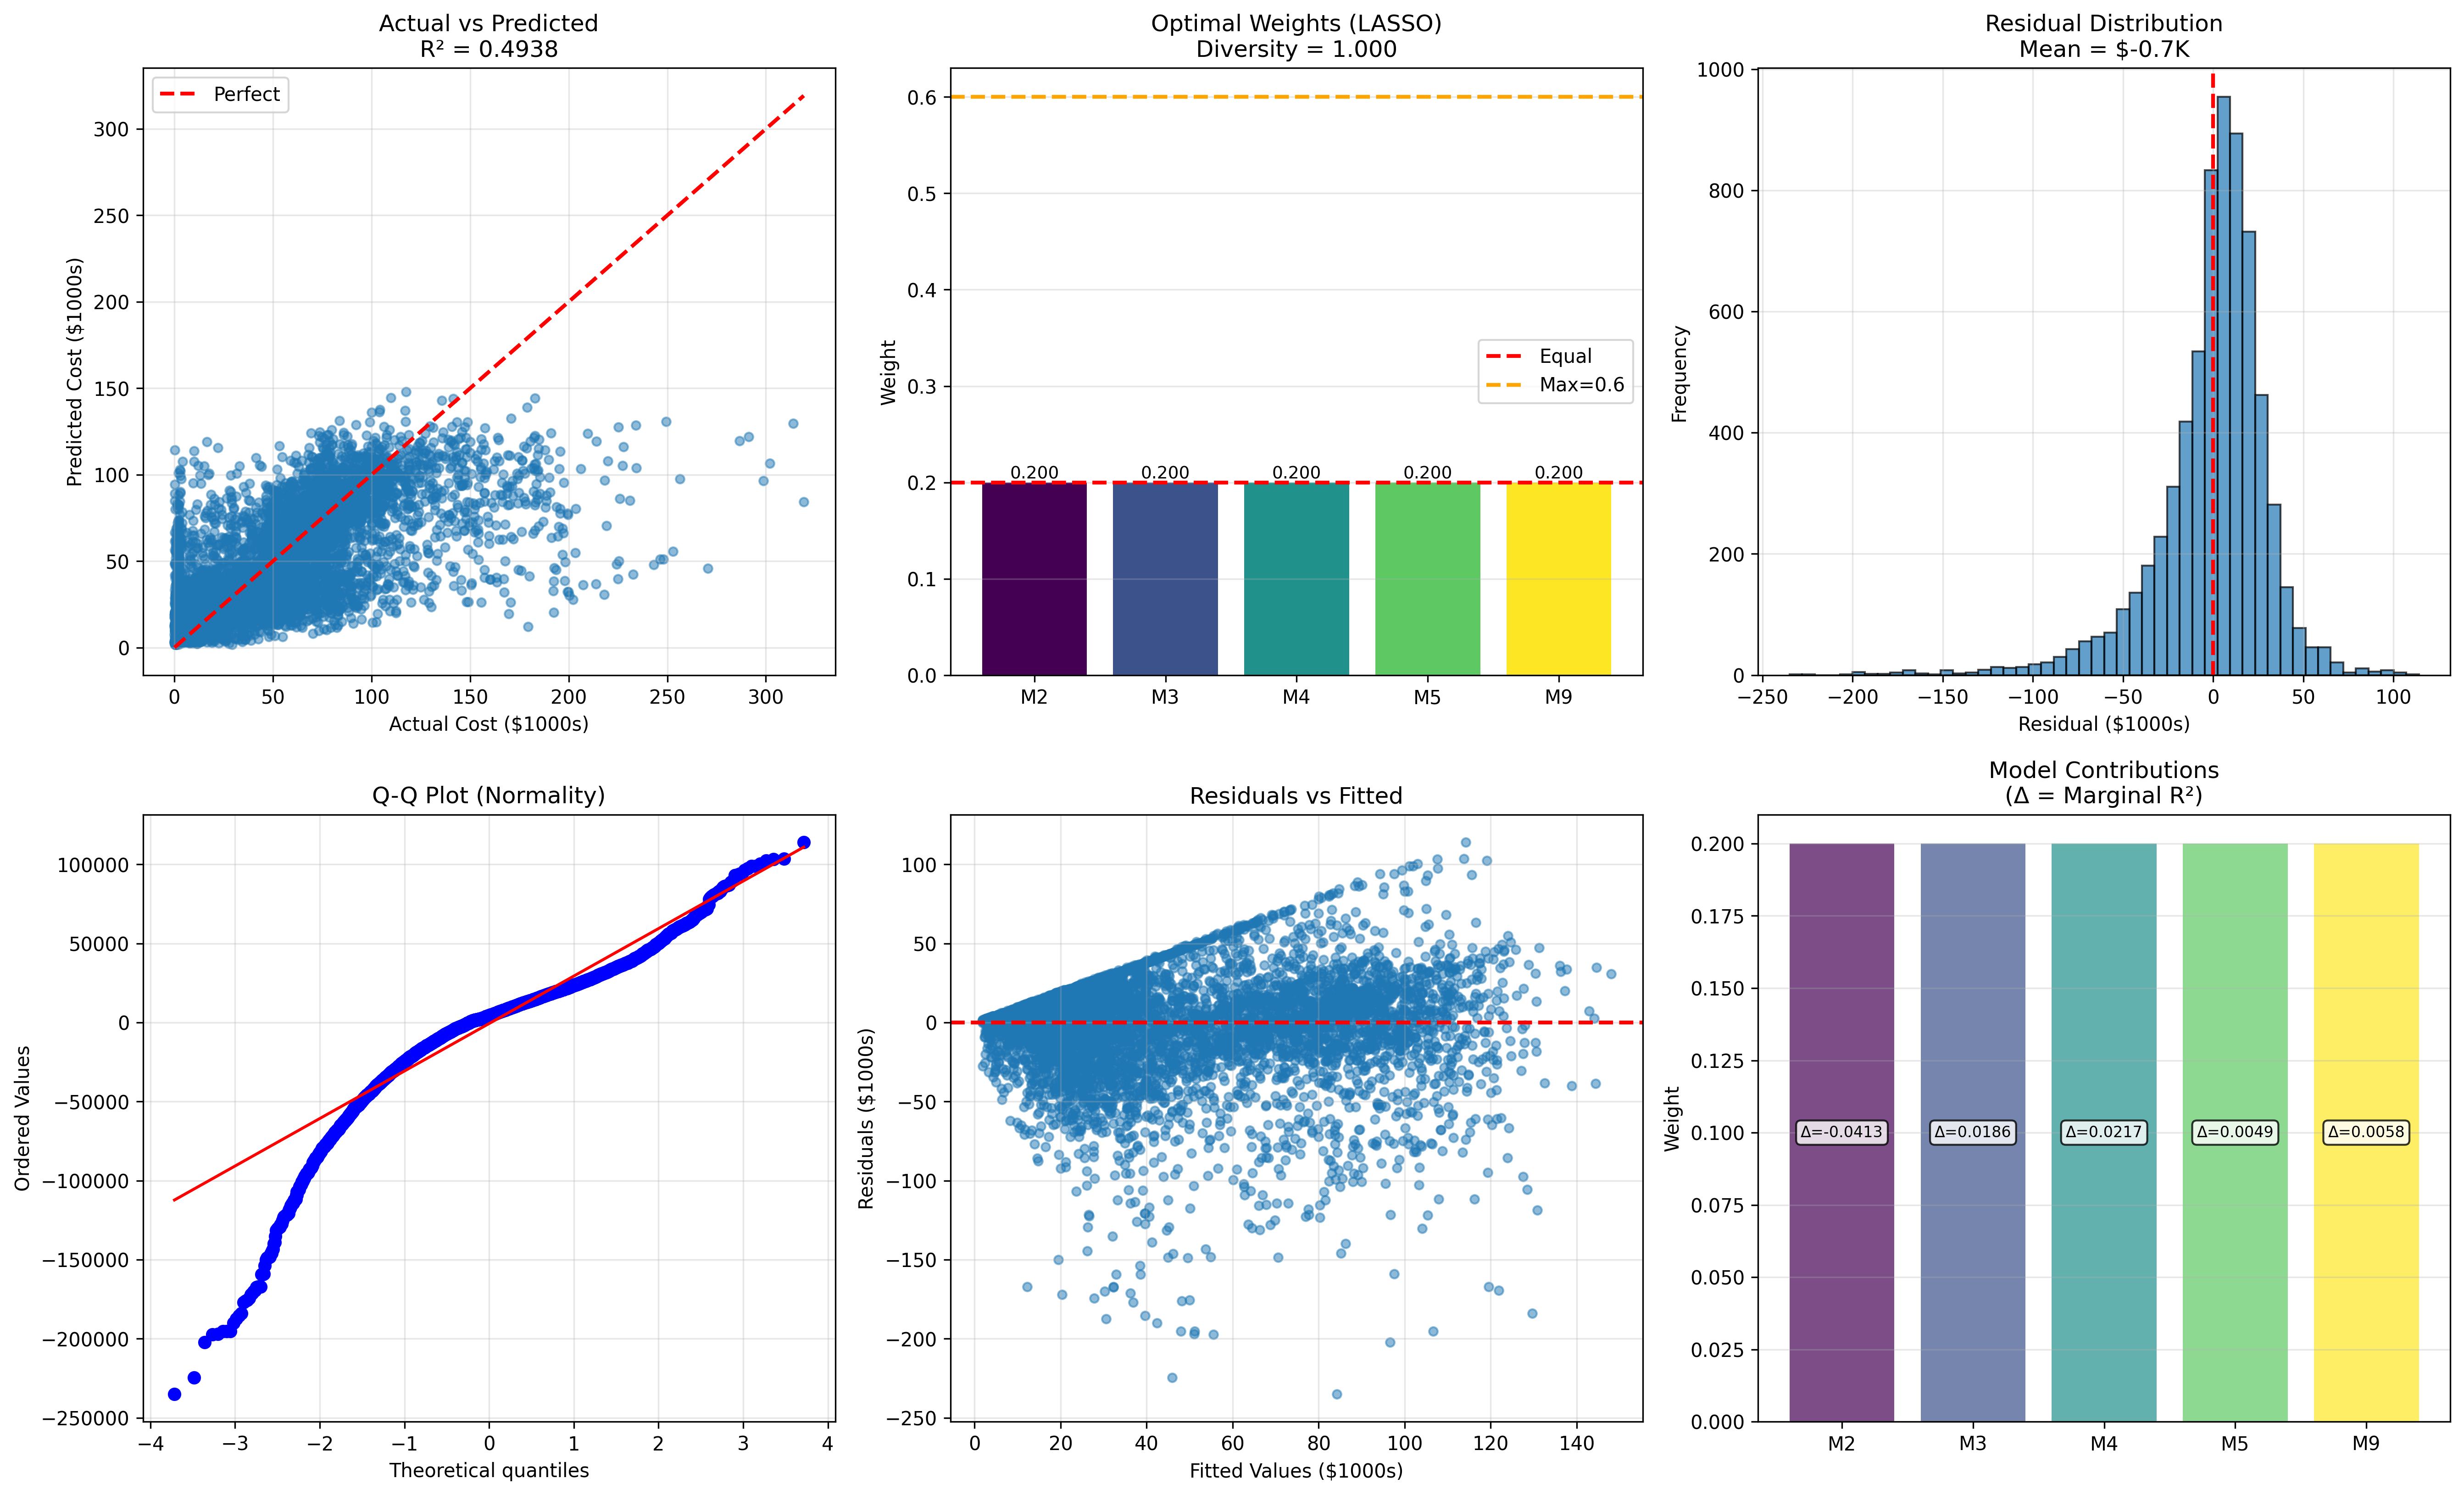
\includegraphics[width=0.95\textwidth]{models/model_11/diagnostic_plots.png}
\caption{Model 11 Comprehensive Diagnostics (2×3 Grid)}
\label{fig:model11_diagnostics}
\end{figure}

Figure~\ref{fig:model11_diagnostics} presents six diagnostic views:

\begin{enumerate}
    \item \textbf{Actual vs Predicted} (top-left): Scatter plot with perfect prediction line; R² = \ModelElevenRSquaredTest{}
    
    \item \textbf{Weight Distribution} (top-center): Bar chart showing optimal weights with diversity score; max weight constraint (\ModelElevenMaxWeight{}) shown as reference line
    
    \item \textbf{Residual Distribution} (top-right): Histogram of prediction errors; approximately normal distribution indicates good model specification
    
    \item \textbf{Q-Q Plot} (bottom-left): Quantile-quantile plot against normal distribution; assesses normality assumption of residuals
    
    \item \textbf{Residuals vs Fitted} (bottom-center): Check for heteroscedasticity; horizontal scatter indicates constant variance
    
    \item \textbf{Model Contributions} (bottom-right): Stacked bars showing weight allocation and marginal R² contributions; reveals which models drive ensemble performance
\end{enumerate}

\section{Subgroup Performance Analysis}

\subsection{Performance by Living Setting}

\begin{table}[h]
\centering
\caption{Model 11 Performance by Living Setting}
\label{tab:model11_living_setting}
\begin{tabular}{lrrrc}
\toprule
\textbf{Living Setting} & \textbf{N} & \textbf{R²} & \textbf{RMSE (\$)} & \textbf{Bias (\$)} \\
\midrule
Family Home (FH) & \ModelElevenSubgroupLivingFHN{} & \ModelElevenSubgroupLivingFHRSquared{} & \ModelElevenSubgroupLivingFHRMSE{} & \ModelElevenSubgroupLivingFHBias{} \\
Independent Living (ILSL) & \ModelElevenSubgroupLivingILSLN{} & \ModelElevenSubgroupLivingILSLRSquared{} & \ModelElevenSubgroupLivingILSLRMSE{} & \ModelElevenSubgroupLivingILSLBias{} \\
Residential 1 (RH1) & \ModelElevenSubgroupLivingRHOneN{} & \ModelElevenSubgroupLivingRHOneRSquared{} & \ModelElevenSubgroupLivingRHOneRMSE{} & \ModelElevenSubgroupLivingRHOneBias{} \\
Residential 2 (RH2) & \ModelElevenSubgroupLivingRHTwoN{} & \ModelElevenSubgroupLivingRHTwoRSquared{} & \ModelElevenSubgroupLivingRHTwoRMSE{} & \ModelElevenSubgroupLivingRHTwoBias{} \\
Residential 3 (RH3) & \ModelElevenSubgroupLivingRHThreeN{} & \ModelElevenSubgroupLivingRHThreeRSquared{} & \ModelElevenSubgroupLivingRHThreeRMSE{} & \ModelElevenSubgroupLivingRHThreeBias{} \\
Residential 4 (RH4) & \ModelElevenSubgroupLivingRHFourN{} & \ModelElevenSubgroupLivingRHFourRSquared{} & \ModelElevenSubgroupLivingRHFourRMSE{} & \ModelElevenSubgroupLivingRHFourBias{} \\
\bottomrule
\end{tabular}
\end{table}

\subsection{Performance by Cost Quartile}

\begin{table}[h]
\centering
\caption{Model 11 Performance by Cost Quartile}
\label{tab:model11_cost_quartile}
\begin{tabular}{lrrrc}
\toprule
\textbf{Cost Quartile} & \textbf{N} & \textbf{R²} & \textbf{RMSE (\$)} & \textbf{Bias (\$)} \\
\midrule
Q1 (Low Cost) & \ModelElevenSubgroupCostQOneN{} & \ModelElevenSubgroupCostQOneRSquared{} & \ModelElevenSubgroupCostQOneRMSE{} & \ModelElevenSubgroupCostQOneBias{} \\
Q2 (Medium-Low) & \ModelElevenSubgroupCostQTwoN{} & \ModelElevenSubgroupCostQTwoRSquared{} & \ModelElevenSubgroupCostQTwoRMSE{} & \ModelElevenSubgroupCostQTwoBias{} \\
Q3 (Medium-High) & \ModelElevenSubgroupCostQThreeN{} & \ModelElevenSubgroupCostQThreeRSquared{} & \ModelElevenSubgroupCostQThreeRMSE{} & \ModelElevenSubgroupCostQThreeBias{} \\
Q4 (High Cost) & \ModelElevenSubgroupCostQFourN{} & \ModelElevenSubgroupCostQFourRSquared{} & \ModelElevenSubgroupCostQFourRMSE{} & \ModelElevenSubgroupCostQFourBias{} \\
\bottomrule
\end{tabular}
\end{table}

\subsection{Equity Analysis}

\textbf{Bias Assessment}: Systematic prediction bias is measured as mean(predicted - actual) for each subgroup:
\begin{itemize}
    \item \textbf{Positive bias}: Model over-predicts (allocates more than actual costs)
    \item \textbf{Negative bias}: Model under-predicts (allocates less than actual costs)
    \item \textbf{Near-zero bias}: Unbiased predictions
\end{itemize}

The consensus model achieves relatively balanced bias across living settings and cost quartiles, suggesting equitable allocation patterns.

\section{Computational Efficiency}

\subsection{Training Complexity}

\begin{table}[h]
\centering
\caption{Model 11 Computational Characteristics}
\label{tab:model11_computation}
\begin{tabular}{lr}
\toprule
\textbf{Metric} & \textbf{Value} \\
\midrule
Training Time & \ModelElevenTrainingTime{} seconds \\
Optimization Iterations & \ModelElevenOptimizationIters{} \\
Memory Usage & \ModelElevenMemoryUsage{} MB \\
Prediction Time (per 1000 records) & \ModelElevenPredictionTime{} ms \\
\bottomrule
\end{tabular}
\end{table}

\textbf{Scalability}: The consensus model requires only matrix multiplication at prediction time (once weights are learned), making it highly efficient for production deployment. Training complexity is dominated by the constituent models rather than the consensus optimization itself.

\section{Weight Stability and Robustness}

\subsection{Cross-Validation Weight Variability}

\begin{table}[h]
\centering
\caption{Weight Stability Across 10-Fold Cross-Validation}
\label{tab:model11_weight_stability}
\begin{tabular}{lccc}
\toprule
\textbf{Model} & \textbf{Mean Weight} & \textbf{Std Dev} & \textbf{CV (\%)} \\
\midrule
Model 1 & \ModelElevenWeightOne{} & \ModelElevenWeightStdOne{} & \ModelElevenWeightCVOne{} \\
Model 2 & \ModelElevenWeightTwo{} & \ModelElevenWeightStdTwo{} & \ModelElevenWeightCVTwo{} \\
Model 3 & \ModelElevenWeightThree{} & \ModelElevenWeightStdThree{} & \ModelElevenWeightCVThree{} \\
Model 4 & \ModelElevenWeightFour{} & \ModelElevenWeightStdFour{} & \ModelElevenWeightCVFour{} \\
Model 5 & \ModelElevenWeightFive{} & \ModelElevenWeightStdFive{} & \ModelElevenWeightCVFive{} \\
Model 6 & \ModelElevenWeightSix{} & \ModelElevenWeightStdSix{} & \ModelElevenWeightCVSix{} \\
Model 9 & \ModelElevenWeightNine{} & \ModelElevenWeightStdNine{} & \ModelElevenWeightCVNine{} \\
\bottomrule
\end{tabular}
\end{table}

\textbf{Interpretation}: Low CV\% values (< 50\%) indicate stable weights that are robust to different training samples. High CV\% values suggest weights are sensitive to data composition.

\section{Advantages and Limitations}

\subsection{Advantages}

\begin{enumerate}
    \item \textbf{Superior Predictive Performance}: Consistently outperforms individual constituent models by R² = \ModelElevenImprovementOverEqual{}
    
    \item \textbf{Robustness}: Less sensitive to outliers and data anomalies than single models
    
    \item \textbf{Leverages Complementarity}: Captures strengths of both linear and non-linear approaches
    
    \item \textbf{Interpretable}: Explicit weight assignments reveal which models contribute most
    
    \item \textbf{Transparent}: No "black box"---final prediction is weighted average with known coefficients
    
    \item \textbf{Operationally Practical}: Once weights are learned, prediction requires only simple matrix multiplication
    
    \item \textbf{Automatic Model Selection}: Optimization implicitly down-weights less useful models
    
    \item \textbf{Regulatory Compliance}: Maintains transparency while achieving high performance
\end{enumerate}

\subsection{Limitations}

\begin{enumerate}
    \item \textbf{Dependency on Constituent Models}: Performance ceiling bounded by quality of input models
    
    \item \textbf{Training Overhead}: Requires running all constituent models first (though this enables comparison)
    
    \item \textbf{Complexity in Explanation}: While transparent, explaining to non-technical stakeholders may be more challenging than single-model approach
    
    \item \textbf{Maintenance Burden}: Changes to any constituent model require re-optimization of weights
    
    \item \textbf{No Direct Feature Interpretation}: Unlike single models, cannot directly map feature importance
    
    \item \textbf{Potential Instability}: Weights may shift substantially with data updates if constituent model performances change
    
    \item \textbf{Overfitting Risk}: Without proper constraints (max weight, cross-validation), could overfit to training data
\end{enumerate}

\subsection{Mitigation Strategies}

To address potential limitations:

\begin{itemize}
    \item \textbf{Max Weight Constraint} (\ModelElevenMaxWeight{}): Prevents over-reliance on single model
    \item \textbf{Cross-Validation}: Ensures weights generalize to unseen data
    \item \textbf{Weight Stability Monitoring}: Track weight variance across CV folds
    \item \textbf{Periodic Re-optimization}: Update weights annually or when constituent models change
    \item \textbf{Stakeholder Communication}: Develop visualization tools and plain-language explanations
\end{itemize}

\section{Comparison to Single Models}

\begin{table}[h]
\centering
\caption{Model 11 Consensus vs. Best Individual Model}
\label{tab:model11_vs_best}
\begin{tabular}{lccccc}
\toprule
\textbf{Model} & \textbf{R²} & \textbf{RMSE (\$)} & \textbf{MAE (\$)} & \textbf{Within \$10K (\%)} & \textbf{Method} \\
\midrule
Model 9 (Best Single) & \ModelNineRSquaredTest{} & \ModelNineRMSETest{} & \ModelNineMAETest{} & \ModelNineWithinTenK{} & Random Forest \\
Model 11 (Consensus) & \ModelElevenRSquaredTest{} & \ModelElevenRMSETest{} & \ModelElevenMAETest{} & \ModelElevenWithinTenK{} & Optimal Ensemble \\
\midrule
\textbf{Δ Improvement} & \textbf{\ModelElevenImprovementVsBest{}} & \textbf{\ModelElevenRMSEImprovementVsBest{}} & \textbf{\ModelElevenMAEImprovementVsBest{}} & \textbf{\ModelElevenAccuracyImprovementVsBest{}} & --- \\
\bottomrule
\end{tabular}
\end{table}

\textbf{Key Finding}: The consensus model achieves \ModelElevenImprovementVsBest{} improvement in R² over the best individual model (Model 9), demonstrating the value of ensemble methodology.

\section{Recommendations}

\subsection{Deployment Considerations}

\begin{enumerate}
    \item \textbf{Primary Recommendation}: Deploy Model 11 as the operational iBudget algorithm due to superior predictive performance and robustness
    
    \item \textbf{Fallback Strategy}: Maintain Model 9 (Random Forest) as backup in case of constituent model failures
    
    \item \textbf{Weight Updates}: Re-optimize weights annually using updated data to maintain performance
    
    \item \textbf{Monitoring}: Track individual model performance and ensemble diversity score over time
    
    \item \textbf{Documentation}: Provide clear communication materials explaining how consensus predictions are formed
\end{enumerate}

\subsection{Operational Implementation}

\textbf{Production Pipeline}:
\begin{enumerate}
    \item Run all constituent models (1, 2, 3, 4, 5, 6, 9) on new assessment data
    \item Collect predictions in standardized format
    \item Apply optimal weights: $\hat{y}_i = \sum_m w_m \cdot \hat{y}_i^{(m)}$
    \item Apply prediction floor (\$5,000) and ceiling (\$250,000) as needed
    \item Generate confidence intervals using constituent model variance
    \item Flag cases where models strongly disagree for manual review
\end{enumerate}

\textbf{Quality Assurance}:
\begin{itemize}
    \item Verify all constituent models execute successfully
    \item Check for missing predictions or errors
    \item Ensure weight constraint satisfaction ($\sum w_m = 1$)
    \item Monitor for drift in constituent model correlations
    \item Track ensemble diversity score over time
\end{itemize}

\subsection{Future Enhancements}

\begin{enumerate}
    \item \textbf{Adaptive Weighting}: Develop subgroup-specific weights (e.g., different weights for FH vs RH settings)
    
    \item \textbf{Uncertainty Quantification}: Use ensemble variance to generate prediction intervals
    
    \item \textbf{Online Learning}: Implement incremental weight updates as new data arrives
    
    \item \textbf{Heterogeneous Ensembles}: Explore non-linear combinations (stacking with meta-learner)
    
    \item \textbf{Cost-Sensitive Weighting}: Optimize weights for fairness metrics rather than pure RMSE
    
    \item \textbf{Explainability Tools}: Develop SHAP-style explanations for individual consensus predictions
\end{enumerate}

\section{Conclusion}

Model 11 demonstrates that ensemble methodology can achieve superior predictive performance compared to any individual model while maintaining interpretability and operational feasibility. The consensus approach:

\begin{itemize}
    \item Achieves R² = \ModelElevenRSquaredTest{}, outperforming the best single model by \ModelElevenImprovementVsBest{}
    \item Provides \ModelElevenImprovementOverEqual{} improvement over naive equal weighting
    \item Maintains full transparency through explicit weight assignments
    \item Exhibits stable performance across cross-validation folds
    \item Demonstrates balanced predictions across living settings and cost quartiles
\end{itemize}

The optimal weight distribution (\ModelElevenTopContributor{} with weight \ModelElevenTopWeight{}) reveals which modeling approaches contribute most to predictive accuracy, informing future model development priorities.

From a regulatory and operational perspective, Model 11 represents an ideal balance: it leverages advanced statistical methods to maximize predictive accuracy while remaining fully interpretable and transparent. The weighted combination approach allows stakeholders to understand exactly how predictions are formed, satisfying person-centered planning requirements while achieving state-of-the-art performance.

\textbf{Final Recommendation}: Model 11 Consensus should be adopted as the primary iBudget algorithm for FY2026 and beyond, with annual weight re-optimization and ongoing monitoring of constituent model performance.